%%%%%%%%%%%%%%%%%%%%%%%%%%%%%%%%%%%%%%%%%%%%%%%%%%%%%%%%%%%%%%%%%%%%%%%%%%%%%%%%
%%%%%%%%%%%%%%%%%%%%%%%%%%%%%%%%%%%%%%%%%%%%%%%%%%%%%%%%%%%%%%%%%%%%%%%%%%%%%%%%
%%                           AUTHOR: BIBEKANANDA DATTA                        %%
%%                               (C) MARCH 2024                               %%
%%                      PhD STUDENT, MECHANICAL ENGINEERING                   %%
%%                           JOHNS HOPKINS UNIVERSITY                         %%
%%%%%%%%%%%%%%%%%%%%%%%%%%%%%%%%%%%%%%%%%%%%%%%%%%%%%%%%%%%%%%%%%%%%%%%%%%%%%%%%
%%%%%%%%%%%%%%%%%%%%%%%%%%%%%%%%%%%%%%%%%%%%%%%%%%%%%%%%%%%%%%%%%%%%%%%%%%%%%%%%
%%             PLEASE CHECK THE README.md FILE BEFORE YOU PROCEED             %%
%%              it may be convenient to read this file on GitHub              %%
%%   GitHub: https://github.com/bibekananda-datta/JHU-Dissertation-Template   %%
%% template hosted on this GitHub repository is likely to be the most updated %%
%%%%%%%%%%%%%%%%%%%%%%%%%%%%%%%%%%%%%%%%%%%%%%%%%%%%%%%%%%%%%%%%%%%%%%%%%%%%%%%%

%%%%%%%%%%%%%%%%%%%%%%%%%%%%%%%%%%%%%%%%%%%%%%%%%%%%%%%%%%%%%%%%%%%%%%%%%%%%%%%%
% This is an unofficial dissertation template for Johns Hopkins University.
% As of March 31, 2024, the template follows the dissertation formatting 
% requirements provided by the  Johns Hopkins University Sheridan Library.
% It is the user's responsibility to ensure that the current requirements are 
% followed: https://www.library.jhu.edu/library-services/electronic-theses-dissertations/formatting-requirements/
%%%%%%%%%%%%%%%%%%%%%%%%%%%%%%%%%%%%%%%%%%%%%%%%%%%%%%%%%%%%%%%%%%%%%%%%%%%%%%%%
%%%%%%%%%%%%%%%%%%%%%%%%%%%%%% VERSION HISTORY %%%%%%%%%%%%%%%%%%%%%%%%%%%%%%%%%
% The report class-based template was created by R. Jacob Vogelstein in May 2007
% Updated by Noah J. Cowan on March 01, 2010
% Updated by Brian D. Weitzner on April 29, 2014 
% Updated by John Muschelli on January 29, 2016 
% Updated by Leonardo Collado Torres on April 13, 2016 
% Updated by John Clayton in December 2019
% Last Updated by Bibekananda Datta on March 31, 2024
%%%%%%%%%%%%%%%%%%%%%%%%%%%%%% VERSION HISTORY %%%%%%%%%%%%%%%%%%%%%%%%%%%%%%%%%


%%%% REPORT CLASS with 12 pt font and onesided printing (book class also works)
\documentclass[12pt,letterpaper]{report} 

%%%%%%%%%%%%%%%%%%%%%%%%%%%%%%%%%%%%%%%%%%%%%%%%%%%%%%%%%%%%%%%%%%%%%%%%%%%%%%%%
%% if possible, make your formatting changes here through the variables 
%%%%%%%%%%%%%%%%%%%%%% LIST OF VARIABLES FOR FORMATTING %%%%%%%%%%%%%%%%%%%%%%%%

%%%% JH Library requirement (DO NOT CHANGE)
\def\GlobalMargin{1.0in}                    % margin on all sides
\def\PrintingOffset{0.5in}                  % additional left margin for the printed copy
\def\MainTextSpacing{\doublespacing}        % double-spaced main text


%%%% ADDITIONAL PATHS and FILES
\def\FigurePath{figures}                    % subdirectory for the figure files
\def\BibFileName{thesis.bib}                % name of BibLaTeX-compatible bib file 


\def\FontPackage{lmodern}                   % default font package

\def\HyperlinkColor{blue}                   % color for hyperlinks


%%%% FONT SIZE and TYPESET for DIFFERENT HEADINGS
%% check here for details: https://en.wikibooks.org/wiki/LaTeX/Fonts
%% font format for thesis title
\def\TitleFont{\Large\bfseries\singlespacing\MakeUppercase}  

%% font for chapter, section, subsection, and subsubsection heading
\def\NoSectionLevel{3}                      % 3 levels => section to subsubsection
\def\ChapterFont{\Large\bfseries\singlespacing} 
\def\SectionFont{\large\bfseries\singlespacing} 
\def\SubsectionFont{\normalsize\bfseries\singlespacing}  
\def\SubsubsectionFont{\normalsize\itshape\singlespacing} 


%%%% PARAGRAPH
\def\ParagraphSpacing{\baselineskip}        % spacing between paragraph
\def\ParagraphIndent{0 pt}                  % indentation at the beginning of the paragraph


%% CAPTION
\def\CaptionFontSize{small}                 % caption font size
\def\CaptionLabelFontType{bf}               % boldface label for captions
\def\CaptionSeparator{colon}                % separates caption label from caption text
\def\CaptionSpacing{1.0}                    % single-spaced captions
\def\FigureToCaption{0 pt}                  % spacing between the figure and the caption


%%%% GLOBAL SPACING for TABLES
\def\GlobalTableSpacing{1.5}                % global spacing parameter for table


%%%% HEADER AND FOOTER SETTING
\def\HeaderHeight{30 pt}                    % height of the chapter header
\def\HeaderSpace{12 pt}                     % space between header and the following text

\def\FootnoteSpacing{\baselineskip}         % spacing between footnotes


%%%% BIBLIOGRAPHY ITEMS
\def\BibTextSpacing{\singlespacing}         % single-spaced bibliography
\def\BibItemSpacing{\baselineskip}          % spacing between bibliographic items in reference


%%%% CHAPTER QUOTE (EPIGRAPH PACKAGE)
\def\ChapQuoteFontSize{\small}              % font size of chapter quotes
\def\ChapQuoteLocation{flushright}          % location of chapter quote
\def\ChapQuoteTextShape{\itshape}           % font shape for quotes
\def\ChapQuoteAuthorTextShape{\scshape}     % font shape for quote author
\def\MaxQuoteWidth{0.65\textwidth}          % width epigraph-based quotes in chapter



%%%% SECTION LEVELS and TOC APPEARANCE
\def\NoTOCLevel{2}                          % no of levels showed in the table of contents
\def\TOCIndent{0 pt}                        % indentation in the list of figs and tables
%% 3 levels mean: section to subsubsection.. decrease if you want to show less in TOC


%%%% TOC SPACING of different section levels (chapter to subsubsection)
\def\TOCTextSpacing{\singlespacing}         % single spacing for TOC texts
\def\ChapTOCSpacing{\baselineskip}          % spacing between chapters
\def\SecTOCSpacing{0.5\baselineskip}        % spacing between sections
\def\SubsecTOCSpacing{0.3\baselineskip}     % ... between subsections
\def\SubsubsecTOCSpacing{0.3\baselineskip}  % ... between subsubsections
\def\LOTItemSpacing{\baselineskip}          % spacing between LOT/LOF items



%%%% ADHOC HEIGHT ADJUSTMENT VARIABLES for consistent typesettings
%% following numbers are found by trial and error to compensate 
%% for the default spacing around different LaTeX environments.
%% unless you find inconsistent formatting, you may not need to change these
\def\TitleTopSpacing{-\HeaderHeight-\HeaderSpace}   % top height adjustment for thesis title
\def\BeforeTOCTitleSpacing{-42 pt}          % space before TOC title
\def\AfterTOCTitleSpacing{34 pt}            % space after TOC title
\def\AfterLOTTitleSpacing{34 pt}            % space after LOT/ LOF title

\def\NumChapterTopMargin{-64 pt}            % space before numbered chapter label
\def\UnNumChapterTopMargin{-85 pt}          % space before unnumbered chapter label
\def\ChapLabelToTitle{-27 pt}               % space between chapter label to title 
\def\ChapTitleToText{24 pt}                 % space between the chapter title and the following text
\def\SpaceBeforeQuote{-20 pt}               % white space before quote

%%%% if you want to change any of the heights, adjust using a ruler:
% \usepackage[unit=in,type=upperleftT,color=red,showframe]{fgruler}

%%%%%%%%%%%%%%%%%%%% END LIST OF VARIABLES FOR FORMATTING %%%%%%%%%%%%%%%%%%%%%%


%%%%%%%%%%%%%%%%%%%%%%%%%%%%%%%%%%%%%%%%%%%%%%%%%%%%%%%%%%%%%%%%%%%%%%%%%%%%%%%%
%% add packages as needed but sometimes the order of the packages matters.
%% you may have to change the options of the biblatex package for the bibliography.
%%%%%%%%%%%%%%%%%%%%%%%%%%%%%%% LaTeX PACKAGES %%%%%%%%%%%%%%%%%%%%%%%%%%%%%%%%%

%%%% SOME PRE-REQUISITE PACKAGES
\usepackage[utf8]{inputenc}                 % for encoding input character (required)
\usepackage[american]{babel}                % for different language typography
\usepackage[T1]{fontenc}                    % for font encoding


%%%% DEFAULT FONT (you can specify other fonts - compatibility could be an issue)
\usepackage{\FontPackage}


%%%% COMMON MATH PACKAGES
\usepackage{amsfonts,amssymb,amsmath,amsthm,autobreak,
    cancel,dsfont,mathtools,mathbbol,mathrsfs,siunitx,upgreek}


%%%% TABLE-RELATED PACKAGES
\usepackage{booktabs,longtable,dcolumn,makecell,
    multicol,multirow,tabularx,xltabular,rotating}


%%%% package for micro-typography (you can define more settings)
%% see details here: https://www.khirevich.com/latex/microtype/
\usepackage[activate={true,nocompatibility}]{microtype}



%%%% BIBLIOGRAPHIC PACKAGE (change the style or other options if you need to)
%% Nature style bibliography
\usepackage[backend=biber, defernumbers=true, style=nature, maxnames=99,
     date=year, isbn=false, url=false, doi=true]{biblatex}

%% APA style
% \usepackage[backend=biber, defernumbers=true, style=apa, maxnames=99,
%     isbn=false, url=false, doi=true]{biblatex}

%% IEEE style
% \usepackage[backend=biber,style=ieee,defernumbers=true,maxnames=99, 
%     date=year, isbn=false, url=false, doi=true]{biblatex}



%%%% OTHER PACKAGES AND OPTIONS
\usepackage[pagewise,mathlines]{lineno}     % line numbers for drafting
\usepackage[ruled]{algorithm2e}             % to manage algorithm environment
\usepackage[titletoc]{appendix}             % to manage appendix chapters
\usepackage{blindtext}                      % to generate random filler texts
\usepackage{calc}                           % to set arithmetic arguments for spacing
\usepackage{caption}                        % to manage captions
\usepackage{comment}                        % to comment a large amount of text as env
\usepackage{epigraph,varwidth}              % for managing quotes
\usepackage{enumitem}                       % to manage list environment
\usepackage{float}                          % to manage floating environment
% footnote environment management
\usepackage[bottom,multiple,hang,flushmargin]{footmisc}      
\usepackage{graphicx,wrapfig}               % to manage images
\usepackage{geometry}                       % to manage margins and page format
\usepackage{glossaries}                     % to add glossaries
\usepackage{fancyhdr}                       % for header/ footer settings
\usepackage[dvipsnames]{xcolor}             % color-related package
\usepackage[a-1b]{pdfx}                     % to generate PDF/A file (add before hyperref)
\usepackage[pdfa]{hyperref}                 % for hyperlink management 
\usepackage[all]{hypcap}                    % for captions on the side of figures
\usepackage{ifthen}                         % if-then statement in LaTeX code
\usepackage{lscape}                         % landscape mode
\usepackage{listings,minted}                % to include codes 
\usepackage{csquotes}                       % yet another package to manage quote
\usepackage{setspace}                       % sets space between lines
\usepackage{seqsplit}                       % splits long character sequence
\usepackage[rightcaption]{sidecap}          % for sideway captions
\usepackage{tocloft}                        % to manage table of contents, etc.
\usepackage{textcomp}                       % text companion fonts in TS1
\usepackage[absolute]{textpos}              % position text at certain location
\usepackage{titlesec}                       % managing different title environments
\usepackage[final]{pdfpages}                % to insert pdf pages
\usepackage{parskip}                        % default spacing around environments
\usepackage{tikz}                           % drawing related package
\usepackage{subcaption}                     % individual panel and caption

%% add more packages and/or change options of the packages as needed
%%%%%%%%%%%%%%%%%%%%%%%%%%%%%% END LaTeX PACKAGES %%%%%%%%%%%%%%%%%%%%%%%%%%%%%

\usepackage{svg}

%%%%%%%%%%%%%%%%%%%%%%%%%%%%%%%%%%%%%%%%%%%%%%%%%%%%%%%%%%%%%%%%%%%%%%%%%%%%%%%
%% specifying direct package options related to document formatting
%%%%%%%%%%%%%%%%%%%%%%%%%%%%%% PACKAGE OPTIONS %%%%%%%%%%%%%%%%%%%%%%%%%%%%%%%%

%%%% GRAPHICX package
\graphicspath{{\FigurePath/}}


%%%% GEOMETRY PACKAGE: margin settings required by JH library 
\geometry{letterpaper, margin=\GlobalMargin, bindingoffset=\PrintingOffset, 
    nomarginpar, includehead, headheight=\HeaderHeight, 
    headsep=\HeaderSpace, includefoot, heightrounded}
%% you can add showframe option to see how the layout looks like


%%%% HYPERREF PACKAGE
\hypersetup{linktocpage, unicode, linktoc=all, colorlinks=true, 
    citecolor=\HyperlinkColor, filecolor=\HyperlinkColor, 
    linkcolor=\HyperlinkColor, urlcolor=\HyperlinkColor}
\urlstyle{rm}           % removes default \texttt style for hyperlinks


%%%% CAPTION PACKAGE
\captionsetup{belowskip=\FigureToCaption, font=\CaptionFontSize, 
    labelfont=\CaptionLabelFontType, labelsep=\CaptionSeparator,
    font={stretch=\CaptionSpacing}, hypcap=true} 


%%%% BIBLATEX: bibliography package settings
\addbibresource{\BibFileName}           % name of the bib file 
% \DeclareFieldFormat{titlecase}{\MakeSentenceCase*{#1}}
\AtBeginBibliography{\urlstyle{rm}}     % roman font family for URL (DOI)
\AtBeginBibliography{\vspace*{8pt}}     % add space for single-spaced bib text

%% the following block ensures articles are sentence case 
%% but the journal names are title case 
\DeclareFieldFormat{sentencecase}{\MakeSentenceCase{#1}}
\renewbibmacro*{title}{%
  \ifthenelse{\iffieldundef{title}\AND\iffieldundef{subtitle}}
    {}
    {\ifthenelse{\ifentrytype{article}\OR\ifentrytype{inbook}%
      \OR\ifentrytype{incollection}\OR\ifentrytype{inproceedings}%
      \OR\ifentrytype{inreference}}
      {\printtext[title]{%
        \printfield[sentencecase]{title}%
        \setunit{\subtitlepunct}%
        \printfield[sentencecase]{subtitle}}}%
      {\printtext[title]{%
        \printfield[titlecase]{title}%
        \setunit{\subtitlepunct}%
        \printfield[titlecase]{subtitle}}}%
     \newunit}%
  \printfield{titleaddon}}


%%%% separate category for papers to be not cited in the bibliography
\DeclareBibliographyCategory{mypapers}             
\newcommand{\mybibexclude}[1]{\addtocategory{mypapers}{#1}}

%%%%%%%%%%%%%%%%%%%%%%%%%%%% END PACKAGE OPTIONS %%%%%%%%%%%%%%%%%%%%%%%%%%%%%%%


%%%%%%%%%%%%%%%%%%%%%%%%%%%%%%%%%%%%%%%%%%%%%%%%%%%%%%%%%%%%%%%%%%%%%%%%%%%%%%%
%% further tweaking variables for the current consistent document formatting
%%%%%%%%%%%%%%%%%%%%%%%%%%%%% DOCUMENT FORMATTING %%%%%%%%%%%%%%%%%%%%%%%%%%%%%%

\setcounter{tocdepth}{\NoTOCLevel}                  % list depth in ToC
\setcounter{secnumdepth}{\NoSectionLevel}           % section to ... subsubsection


%%%% font size and spacing around the titles of ToC/ LoT/ LoF
\renewcommand{\cfttoctitlefont}{\ChapterFont}
\renewcommand{\cftlottitlefont}{\ChapterFont}
\renewcommand{\cftloftitlefont}{\ChapterFont}

\setlength{\cftbeforetoctitleskip}{\BeforeTOCTitleSpacing}
\setlength{\cftbeforelottitleskip}{\BeforeTOCTitleSpacing}
\setlength{\cftbeforeloftitleskip}{\BeforeTOCTitleSpacing}
\setlength{\cftaftertoctitleskip}{\AfterTOCTitleSpacing}
\setlength{\cftafterlottitleskip}{\AfterLOTTitleSpacing}
\setlength{\cftafterloftitleskip}{\AfterLOTTitleSpacing}


%% tweak to TOC to add 'chapter' to the chapter name instead of a number only
%% set the width of the box based on the longest label name
\renewcommand{\cftchappresnum}{\chaptername\space}
\renewcommand{\cftchapleader}{\cftdotfill{\cftdotsep}}  % dots for chapters too
\setlength{\cftchapnumwidth}{\widthof{\textbf{Appendix~XXX~}}}


\setlength{\cftbeforechapskip}{\ChapTOCSpacing}
\setlength{\cftbeforesecskip}{\SecTOCSpacing}
\setlength{\cftbeforesubsecskip}{\SubsecTOCSpacing}
\setlength{\cftbeforesubsubsecskip}{\SubsubsecTOCSpacing}


%% tweak to LOT and LOF to add 'Table'/ 'Figure' to the table/ figure caption listing
%% to change the distance to the start of the table/ figure title
\newcommand*{\noaddvspace}{\renewcommand*{\addvspace}[1]{}}

\setlength{\cfttabindent}{\TOCIndent}               % indentation from tables in LoT
\renewcommand{\cfttabpresnum}{\bfseries Table }
\setlength{\cfttabnumwidth}{\widthof{\textbf{Table~999.999~}}}
\setlength{\cftbeforetabskip}{\LOTItemSpacing}      % spacing between each item
\addtocontents{lot}{\protect\noaddvspace}


\setlength{\cftfigindent}{\TOCIndent}               % indentation from figures in LoF
\renewcommand{\cftfigpresnum}{\bfseries Figure }
\setlength{\cftfignumwidth}{\widthof{\textbf{Figure~999.999~}}}
\setlength{\cftbeforefigskip}{\LOTItemSpacing}      % spacing between each item
\addtocontents{lof}{\protect\noaddvspace}



%%%% TITLESEC: settings for chapter label and title
\titleformat{\chapter}[display]{\ChapterFont}
    {\chaptertitlename\ \thechapter}{\ChapLabelToTitle}{\ChapterFont}

\titlespacing*{\chapter}{0pt}{\NumChapterTopMargin}{\ChapTitleToText} 

\titlespacing*{name=\chapter,numberless}{0pt}{\UnNumChapterTopMargin}
    {\ChapTitleToText}


%%%% TITLESEC: settings for sections, subsection, ... heading format
\titleformat*{\section}{\SectionFont}
\titleformat*{\subsection}{\SubsectionFont}
\titleformat*{\subsubsection}{\SubsubsectionFont}
%% if you had more levels then add settings for paragraph and subparagraph


%% to customize space around section headings, use the following command:
% \titlespacing*{environment-name}{space-left}{space-before}{space-after}


%%%% PARSKIP: for paragraph (and not title) spacing, roughly speaking
\renewcommand{\arraystretch}{\GlobalTableSpacing}   % spacing inside table
\setlength{\parskip}{\ParagraphSpacing}             % paragraph skip
\setlength{\parindent}{\ParagraphIndent}            % paragraph indentation
\setlength{\bibitemsep}{\BibItemSpacing}            % bib item separation 
\setlength{\footnotesep}{\FootnoteSpacing}          % separation between footnote

%%%%%%%%%%%%%%%%%%%%%%%%%%% END DOCUMENT FORMATTING %%%%%%%%%%%%%%%%%%%%%%%%%%%


%%%%%%%%%%%%%%%%%%%%%%%%%%%%% TITLE PAGE MACROS %%%%%%%%%%%%%%%%%%%%%%%%%%%%%%%

\newcommand{\ThesisTitle}[1]{           % prints thesis title
    \vspace*{\TitleTopSpacing}
    {\TitleFont {#1} \par}
}

\newcommand{\ThesisAuthor}[1]{          % prints by ... thesis author in two lines
    by \\ #1 \\
}      

\newcommand{\ThesisStatement}[2]{       % prints thesis or dissertation statement 
    A {#1} submitted to The Johns Hopkins University in conformity \\
    with the requirements for the degree of {#2}
}

\newcommand{\Location}{Baltimore, Maryland}     % prints location

\newcommand{\ThesisDate}[2]{#1 #2}              % prints thesis submission date 

\newcommand{\ThesisCopyright}[2]{               % prints the optional copyright statement
\begin{textblock*}{\textwidth}(\GlobalMargin +\PrintingOffset,9in)
    \copyright\ {#1} {#2} \\ All rights reserved
\end{textblock*}
\null
}

%%%%%%%%%%%%%%%%%%%%%%%%%%% END TITLE PAGE MACROS %%%%%%%%%%%%%%%%%%%%%%%%%%%%%


%%%%%%%%%%%%%%%%%%%%%%%%%%%%%% OTHER MACROS %%%%%%%%%%%%%%%%%%%%%%%%%%%%%%%%%%%

%%%% UNNUMBERED CHAPTERS, SECTION, and SUBSECTION COMMAND for ADDING to TOC
%% removes the 'Chapter #' title while keeping it listed in the TOC
\newcommand\chap[1]{%
    \chapter*{#1}%
    \markboth{#1}{}
    \addcontentsline{toc}{chapter}{#1}}
  
%% removes the 'Section #' title while keeping it listed in the TOC
\newcommand\sect[1]{%
    \phantomsection
    \section*{#1}%
    \addcontentsline{toc}{section}{#1}}
  
%% removes the 'Subsection #' title while keeping it listed in the TOC
\newcommand\subsect[1]{%
    \phantomsection
    \subsection*{#1}%
    \addcontentsline{toc}{subsection}{#1}}

%% removes the 'Subsubsection #' title while keeping it listed in the TOC
\newcommand\subsubsect[1]{%
    \phantomsection
    \subsubsection*{#1}%
    \addcontentsline{toc}{subsubsection}{#1}}

%%%% KEYWORDS for abstract
\newcommand{\keywords}[1]{	
    \textbf{Keywords:} {#1}
}

%%%% TOCLOFT: modified macros/ commands for printing ToC, LoF, LoT
\newcommand{\mytableofcontents}{
    \clearpage
    \renewcommand{\contentsname}{Table of Contents}
    \tableofcontents
    \clearpage
}
%
\newcommand{\mylistoffigures}{
    \clearpage \phantomsection
    \addcontentsline{toc}{chapter}{List of Figures}
    \listoffigures
    \clearpage
}
%
\newcommand{\mylistoftables}{
    \clearpage \phantomsection
    \addcontentsline{toc}{chapter}{List of Tables}
    \listoftables
    \clearpage
}

%%%% IN-TEXT MACROS for own notes (you can define more)
\newcommand{\COMMENT}{\textcolor{red}}
\newcommand{\ADDCITATION}{\COMMENT{(ADD CITATION)}}

%%%%%%%%%%%%%%%%%%%%%%%%%%%% END OTHER MACROS %%%%%%%%%%%%%%%%%%%%%%%%%%%%%%%%%



%%%%%%%%%%%%%%%%%%%%%%%%%%%%%%%%%%%%%%%%%%%%%%%%%%%%%%%%%%%%%%%%%%%%%%%%%%%%%%%
%% only if you plan on using chapter quotes, you may need epigraph settings
%%%%%%%%%%%%%%%%%%%%%%%%%%%%% EPIGRAPH SETTINGS %%%%%%%%%%%%%%%%%%%%%%%%%%%%%%%

\setlength{\epigraphwidth}{\MaxQuoteWidth}              % max width of chapter epigraph
\renewcommand{\epigraphflush}{\ChapQuoteLocation}       % chapter epigraph on right 
\renewcommand{\epigraphsize}{\ChapQuoteFontSize}        % font size for chapter epigraph
\renewcommand{\textflush}{\ChapQuoteLocation}
\renewcommand{\sourceflush}{\ChapQuoteLocation}
\newcommand{\epitextfont}{\ChapQuoteTextShape}          % quote font shape
\newcommand{\episourcefont}{\ChapQuoteAuthorTextShape}  % quote author name shape

%% following settings put variable width underline between quote and author
\makeatletter
\setlength{\beforeepigraphskip}{\SpaceBeforeQuote}
\newsavebox{\epi@textbox}
\newsavebox{\epi@sourcebox}
\newlength\epi@finalwidth
\renewcommand{\epigraph}[2]{%
    \vspace{\beforeepigraphskip}
    {\epigraphsize\begin{\epigraphflush}
    \epi@finalwidth=\z@
    \sbox\epi@textbox{%
        \varwidth{\epigraphwidth}
        \begin{\textflush}\epitextfont#1\end{\textflush}
        \endvarwidth
   }%
    \epi@finalwidth=\wd\epi@textbox
    \sbox\epi@sourcebox{%
        \varwidth{\epigraphwidth}
        \begin{\sourceflush}\episourcefont#2\end{\sourceflush}%
        \endvarwidth
   }%
    \ifdim\wd\epi@sourcebox>\epi@finalwidth 
        \epi@finalwidth=\wd\epi@sourcebox
    \fi
   \leavevmode\vbox{
        \hb@xt@\epi@finalwidth{\hfil\box\epi@textbox}
        \vskip 1ex         % gap between quote and rule
        \hrule height \epigraphrule
        \vskip 1ex         % gap between rule and author
        \hb@xt@\epi@finalwidth{\hfil\box\epi@sourcebox}
   }%
   \end{\epigraphflush}
   \vspace{\afterepigraphskip}}}
\makeatother

%%%%%%%%%%%%%%%%%%%%%%%%%%% END EPIGRAPH SETTINGS %%%%%%%%%%%%%%%%%%%%%%%%%%%%%


%%% define custom settings for other packages here (algorithm/ listing, etc.)


%%%%%%%%%%%%%%%%%%%%%%%%%%%%%%%%%%%%%%%%%%%%%%%%%%%%%%%%%%%%%%%%%%%%%%%%%%%%%%%
%% these are just some examples; add more settings, macros, environments, etc. 
%%%%%%%%%%%%%%%%%%%%%%%%%%%%%% MATH MACROS %%%%%%%%%%%%%%%%%%%%%%%%%%%%%%%%%%%%

%% basic settings for math environment
\allowdisplaybreaks[1]                  % page break for long equations
\numberwithin{equation}{chapter}        % eqn no with chapter label
\setcounter{MaxMatrixCols}{20}          % no of maximum columns in matrix

%% custom math macros
\newcommand{\dC}{$^{\circ}$C}           % degree celsius symbol
\newcommand{\vect}[1]{\mathbf{#1}}      % boldface for vectors and tensors
\DeclareMathOperator{\T}{{\top}}        % transpose of a matrix/ tensor
\DeclareMathOperator{\tr}{tr}           % trace of a matrix
\DeclareMathOperator{\divg}{div}        % divergence of vector and tensor
\DeclareMathOperator{\grad}{grad}       % gradient of vector and tensor
\DeclareMathOperator{\curl}{curl}       % curl of vector and tensor

%% theorem-style remark environment (custom)
\theoremstyle{definition}
\newtheorem{remark}{Remark}
\counterwithin{remark}{chapter}
%%%%%%%%%%%%%%%%%%%%%%%%%%%%% END MATH MACROS %%%%%%%%%%%%%%%%%%%%%%%%%%%%%%%%%


%%%%%%%%%%%%%%%%%%%%%%%%%%%%%%%%%%%%%%%%%%%%%%%%%%%%%%%%%%%%%%%%%%%%%%%%%%%%%%%%%%%%%%%%%%%%%%%%%%%%%%%%%%%%%%%%%%%%%%%%%%%%%%%%%%%%%%%%%%%%%%%%%%%%%%%%



%Paper commands
\newcommand{\Dkinbkg}{\ensuremath{\mathcal{D}^\text{kin}_\text{bkg}}\xspace}
\newcommand{\RelMassErr}{\ensuremath{\delta m_{4\Pell}/m_{4\Pell}}\xspace}
\newcommand{\mZone}{\ensuremath{m(\PZ_{1})}\xspace}
\newcommand{\mZ}{\ensuremath{{m}_{\PZ}}\xspace}
\newcommand{\ggZZ}{\ensuremath{\Pg\Pg \to \PZ\PZ}\xspace}
\newcommand{\Hfourl}{\ensuremath{\PH \to 4\Pell}\xspace}
\newcommand{\Eq}[1]{Eq.~(\ref{#1})}
\newcommand{\Eqs}[3]{Eqs.~(\ref{#1}) #3 (\ref{#2})}
\newcommand{\jhugen}{\textsc{JHUGen}\xspace}
\newcommand{\minlo}{\textsc{MINLO}\xspace}
\newcommand{\mela}{\textsc{mela}\xspace}
\newcommand{\hnnlo}{\textsc{hnnlo}\xspace}
\newcommand{\F}{\ensuremath{\cmsSymbolFace{F}}\xspace}
\newcommand{\WW}{\ensuremath{\PW\PW}\xspace}
\newcommand{\ZZ}{\ensuremath{\PZ\PZ}\xspace}
\newcommand{\VVV}{\ensuremath{\cmsSymbolFace{VVV}}\xspace}
\newcommand{\VBF}{\ensuremath{\mathrm{VBF}}\xspace}
\newcommand{\VH}{\ensuremath{\PV\PH}\xspace}
\newcommand{\WH}{\ensuremath{\PW\PH}\xspace}
\newcommand{\ZH}{\ensuremath{\PZ\PH}\xspace}
\newcommand{\tqH}{\ensuremath{\PQt\PQq\PH}\xspace}
\newcommand{\ttH}{\ensuremath{\PQt\PAQt\PH}\xspace}
\newcommand{\bbH}{\ensuremath{\PQb\PAQb\PH}\xspace}
\newcommand{\ggH}{\ensuremath{\Pg\Pg\PH}\xspace}
\newcommand{\ZX}{\ensuremath{\PZ+\PX}\xspace}
\newcommand{\Hboson}{Higgs boson\xspace}
\newcommand{\Hell}{\ensuremath{\PH\to4\Pell}\xspace}
\newcommand{\GH}{\ensuremath{\Gamma_\PH}\xspace}
\newcommand{\Gref}{\ensuremath{\Gamma_0}\xspace}
\newcommand{\GHSM}{\ensuremath{\Gamma_\PH^{\mathrm{SM}}}\xspace}
\newcommand{\mH}{\ensuremath{m_{\PH}}\xspace}
\newcommand{\mell}{\ensuremath{m_{4\Pell}}\xspace}
\newcommand{\bbar}{\ensuremath{\PQb\PAQb}\xspace}
\newcommand{\muF}{\ensuremath{\mu_{\F}}\xspace}
\newcommand{\muV}{\ensuremath{\mu_{\PV}}\xspace}
\newcommand{\Dbkg}{\ensuremath{{\mathcal{D}}_{\text{bkg}}}\xspace}
\newcommand{\Dint}{\ensuremath{{\mathcal{D}}_{\text{int}}}\xspace}
\newcommand{\Dbsi}{\ensuremath{{\mathcal{D}}_{\text{bsi}}}\xspace}
\newcommand{\Dbkgkin}{\ensuremath{{\mathcal{D}}^{\text{kin}}_{\text{bkg}}}\xspace}
\newcommand{\offshell}{off-shell\xspace}
\newcommand{\onshell}{on-shell\xspace}
\newcommand{\HVV}{\ensuremath{\PH\PV\PV}\xspace}
%Analysis Note commands
\newcommand{\Eqss}[4]{Eqs.~(\ref{#1}), (\ref{#2}), #4~(\ref{#3})}
\newcommand\sss{}
\newcommand{\cPe}{\Pe\xspace}
\newcommand{\cPm}{\PGm\xspace}
\newcommand{\ff}{\ensuremath{\cmsSymbolFace{ff}}\xspace}
\newcommand{\ffbar}{\ensuremath{\cmsSymbolFace{f}\cmsSymbolFace{\overline{f}}}\xspace}
\newcommand{\ROOT}{\textsc{ROOT}\xspace}
\newcommand{\aMCATNLO} {\textsc{MG5}\_a\MCATNLO\xspace}
\newcommand{\V}{\ensuremath{\cmsSymbolFace{V}}\xspace}
\newcommand{\VV}{\ensuremath{\cmsSymbolFace{VV}}\xspace}
% \newcommand{\HVV}{\ensuremath{\PH\V\V}\xspace}
\newcommand{\Hff}{\ensuremath{\PH\text{ff}}\xspace}
\newcommand{\Htt}{\ensuremath{\PH\text{tt}}\xspace}
%\newcommand{\Htt}{\ensuremath{\PH\Pt\Pt}\xspace}
\newcommand{\Hgg}{\ensuremath{\PH\Pg\Pg}\xspace}
\newcommand{\HWW}{\ensuremath{\PH\PW\PW}\xspace}
\newcommand{\HZZ}{\ensuremath{\PH\PZ\PZ}\xspace}
% \newcommand{\VH}{\ensuremath{\V\PH}\xspace}
% \newcommand{\tqH}{\ensuremath{\PQt\cPq\PH}\xspace}
% \newcommand{\ZX}{\ensuremath{\PZ+\X}\xspace}
\newcommand{\X}{\ensuremath{\cmsSymbolFace{X}}\xspace}
% \newcommand{\Hboson}{\ensuremath{\PH} boson\xspace}
% \newcommand{\Hell}{\ensuremath{\PH\to4\ell}\xspace}
\newcommand{\qq}{\ensuremath{\Pq\Pq}\xspace}
\newcommand{\usedLumiD}{35.9\fbinv\xspace}
\newcommand{\usedLumiE}{41.5\fbinv\xspace}
\newcommand{\usedLumiF}{59.7\fbinv\xspace}
\newcommand{\usedLumiALL}{138\fbinv\xspace}
% \newcommand{\mell}{\ensuremath{m_{4\ell}}\xspace}
\newcommand{\glufu}{\ensuremath{\Pg\Pg}\xspace}
% \newcommand{\muV}{\ensuremath{\mu_{\V}}\xspace}
\newcommand{\muVVH}{\ensuremath{\mu_{\cmsSymbolFace{vv}\PH}}\xspace}
%
\newcommand{\Dai}{\ensuremath{{\mathcal{D}}_{ai}}\xspace}
% \newcommand{\Dint}{\ensuremath{{\mathcal{D}}_{\mathrm{int}}}\xspace}
\newcommand{\Dintvec}{\ensuremath{{\vec{\mathcal{D}}}_{\mathrm{int}}}\xspace}
\newcommand{\Dgg}{\ensuremath{{\mathcal{D}}_{\glufu}}\xspace}
% \newcommand{\Dbsi}{\ensuremath{{\mathcal{D}}_{\mathrm{bsi}}}\xspace}
\newcommand{\Dcp}{\ensuremath{{\mathcal{D}}_{C\!P}}\xspace}
\newcommand{\DbkgVBFdec}{\ensuremath{{\mathcal{D}}^{{\VBF}+\text{dec}}_{\text{bkg}}}\xspace}
\newcommand{\DbkgVHdec}{\ensuremath{{\mathcal{D}}^{{\VH}+\text{dec}}_{\text{bkg}}}\xspace}
\newcommand{\DjjVBF}{\ensuremath{{\mathcal{D}}^{\VBF}_{\text{2jet}}}\xspace}
\newcommand{\DjjZH}{\ensuremath{{\mathcal{D}}^{\ZH}_{\text{2jet}}}\xspace}
\newcommand{\DjjWH}{\ensuremath{{\mathcal{D}}^{\WH}_{\text{2jet}}}\xspace}
\newcommand{\DjjVH}{\ensuremath{{\mathcal{D}}^{\VH}_{\text{2jet}}}\xspace}
\newcommand{\fA}{\ensuremath{f_{a1}}\xspace}
\newcommand{\fB}{\ensuremath{f_{a2}}\xspace}
\newcommand{\fBc}{\ensuremath{f_{a2}\cos\left(\phi_{a2}\right)}\xspace}
\newcommand{\fC}{\ensuremath{f_{a3}}\xspace}
\newcommand{\fCc}{\ensuremath{f_{a3}\cos\left(\phi_{a3}\right)}\xspace}
\newcommand{\fL}{\ensuremath{f_{\Lambda1}}\xspace}
\newcommand{\fLc}{\ensuremath{f_{\Lambda1}\cos\left(\phi_{\Lambda1}\right)}\xspace}
\newcommand{\fLZg}{\ensuremath{f_{\Lambda1}^{\PZ\gamma}}\xspace}
\newcommand{\fLZgc}{\ensuremath{f_{\Lambda1}^{\PZ\gamma}\cos\left(\phi_{\Lambda1}^{\PZ\gamma}\right)}\xspace}
\newcommand{\fG}{\ensuremath{f_{a3}^{\Pg\Pg\PH}}\xspace}
\newcommand{\fGc}{\ensuremath{f_{a3}^{\Pg\Pg\PH}\cos\left(\phi_{a3}^{\Pg\Pg\PH}\right)}\xspace}
\newcommand{\fT}{\ensuremath{f_\mathrm{CP}^{\Htt}}\xspace}
\newcommand{\fTc}{\ensuremath{f_\mathrm{CP}^{\Htt}\cos\left(\phi_\mathrm{CP}^{\Htt}\right)}\xspace}
\newcommand{\dphijj}{\ensuremath{\Delta\phi_{\rm j\rm j}}\xspace} % was \scriptscriptstyle
\newcommand{\dzm}{\ensuremath{\mathcal D_{\rm 0-}}\xspace} % was \scriptscriptstyle
\newcommand{\dzmqq}{\ensuremath{\mathcal D_{\rm 0-}^{\rm qq}}\xspace} % was \scriptscriptstyle
\newcommand{\fai}{\ensuremath{f_{ai}}}
\newcommand{\pai}{\ensuremath{\phi_{ai}}}
\newcommand{\Offshell}{Off-shell\xspace}
\newcommand{\LC}[1]{\ensuremath{\Lambda_{#1}}\xspace}
\newcommand{\LZGs}{\ensuremath{\LC{1}^{\PZ\gamma}}\xspace}
\newcommand{\AC}[1]{\ensuremath{a_{#1}}\xspace}
\newcommand{\ai}{\ensuremath{\AC{i}}\xspace}
\newcommand{\fLC}[1]{\ensuremath{f_{\Lambda #1}}\xspace}
\newcommand{\fAC}[1]{\ensuremath{f_{a #1}}\xspace}
\newcommand{\fLZGs}{\ensuremath{\fLC{1}^{\PZ\gamma}}\xspace}
\newcommand{\vv}{\ensuremath{\cmsSymbolFace{vv}}\xspace}

%%%%%%%%%%%%%%%%%%%%%%%%%%%%%%%%%%%%%%%%%%%%%%%%%%%%%%%%%%%%%%%%%%%%%%%%%%%%%%%%%%%%%%%%%%%%%%%%%%%%%%%%%%%%%%%%%%%%%%%%%%%%%%%%%%%%%%%%%%%%%%%%%%%%%%%%

\usepackage{feynmp-auto}
\usepackage{lipsum}

%%%%%%%%%%%%%%%%%%%%%%%%% DOCUMENT BEGINS HERE %%%%%%%%%%%%%%%%%%%%%%%%%%%

\begin{document}



%%%% TITLE PAGE
%%%% JHU Dissertation title page (if you are not sure, do not change the formatting)

\begin{titlepage}

%% centered single-spaced title page w/o page numbering
\begin{center} \singlespacing \thispagestyle{empty}       


%%%% thesis title: 1.5 inches from the top of the page
% \ThesisTitle{Measuring properties of the \\Higgs boson utilizing off-shell production in \(H^{(*)} \to ZZ^{(*)} \to 4\ell\) at the \\CERN Large Hadron Collider}

% \ThesisTitle{Measuring properties of the \\Higgs boson utilizing off-shell production in \(\text{H}^{(*)} \to \text{ZZ}^{(*)} \to \mathbf{4\ell}\) at the \\CERN Large Hadron Collider}

\ThesisTitle{MEASURING PROPERTIES OF THE\\HIGGS BOSON UTILIZING ITS\\OFF-SHELL PRODUCTION}

\vspace{1in}                    % gap between the title and the author: approx. 1 inch

\ThesisAuthor{Lucas Kang}         % author name for the thesis

\vspace{1.5in}                  % gap between the author and statement: 1.5 inches

%%%% for masters, change the arguments to: {thesis}{masters program name}
\ThesisStatement{dissertation}{Doctor of Philosophy}  
%% gap between statement and location: approx. 0.5 inch
\vspace{0.5in} \\               

\Location \\                    % prints Baltimore, Maryland as the location
\ThesisDate{August}{2025}        % thesis submission month and year (single-spaced)


%%%% optional copyright statement: approx. 2 inches from the bottom of the page
%% year and name are input argument for copyright statement
\ThesisCopyright{2025}{Lucas Kang}


\end{center}

\end{titlepage}
        

%%%%%%%%%%%%%%%%%%%%%%%%%%%% FRONT MATTER %%%%%%%%%%%%%%%%%%%%%%%%%%%%%%%%

%%%% text spacing, page numbering, and header settings
\MainTextSpacing                            % double spacing for the contents
\pagenumbering{roman}                       % pagination style: Roman numeral
\setcounter{page}{2}                        % page counter starts at roman ii
\pagestyle{fancy}
\renewcommand{\chaptermark}[1]{\markboth{#1}{#1}}
\fancyhead[R]{}               
\fancyhead[L]{\nouppercase \leftmark}       % prints header for unnumbered chap


%%%% MUST ADD ABSTRACT (includes committee as well)
\chap{Abstract} 


%%%% your abstract goes here (word limit: 350)
The Higgs boson is the last observed piece of the Standard Model of particle physics, and due to its couplings to other fundamental particles, provides a promising portal through which we can potentially probe new physics beyond the Standard Model. This thesis revolves around an analysis which incorporates the full Run 2 dataset from the CMS experiment at the LHC to make precision measurements of the Higgs boson, utilizing a combination of its on- and off-shell production. It also set the stage for novel extensions to analysis of Higgs boson production in the off-shell region, so that future endeavors can better constrain coupling strengths between the Higgs boson and other particles in the search for Beyond-the-Standard-Model (BSM) physics. 

\vspace{1in}

%% list of keywords seperated by comma
\keywords{Higgs, boson, precision, measurement, width, off-shell, golden channel, HVV, kappa, anomalous, coupling, Standard Model, SM, BSM, CMS, LHC, CERN.}







% \chap{Thesis Committee}
% %%%%  committee members (add it right after the abstract w/o page break)
% \begin{singlespace}

%     %% if you have co-advisor, add here w/ \vspace{0.1in} as shown below
%     %% alternatively you can use minipage environment to put side-by-side

%     % \vspace{0.3in}
    
%     % \section*{Thesis Committee}

%     % \vspace{0.2in}
    
%     Andrei Gritsan (Advisor) \\
%     \null\quad\quad Professor \\
%     \null\quad\quad Department of Physics\\
%     \null\quad\quad Johns Hopkins University, Baltimore MD 

%     % \section*{Thesis Committee}

%     \vspace{0.1in}
    
%     Morris Swartz\\
%     \null\quad\quad Professor \\
%     \null\quad\quad Department of Physics \\
%     \null\quad\quad Johns Hopkins University, Baltimore, MD 
    
%     \vspace{0.1in}
    
%     Robert Leheny \\
%     \null\quad\quad Professor \\
%     \null\quad\quad Department of Physics \\
%     \null\quad\quad Johns Hopkins University, Baltimore, MD 

%     \vspace{0.1in}

%     Kobe Marshall-Stevens \\
%     \null\quad\quad J.J. Sylvester Assistant Professor \\
%     \null\quad\quad Department of Mathematics \\
%     \null\quad\quad Johns Hopkins University, Baltimore, MD 
    
%     \vspace{0.1in}
    
%     Toni Šćulac \\
%     \null\quad\quad Assistant Professor \\
%     \null\quad\quad Faculty of Science \\
%     \null\quad\quad University of Split, Split, Croatia 
    
%     % \vspace{0.1in}
    
%     % Dr. Jim Gates \\
%     % Professor\\
%     % Department of Physics \\
%     % University of Maryland, College Park, MD
    
%     % \vspace{0.1in}
    
%     % Dr. Ulrich Heintz \\
%     % Professor\\
%     % Department of Physics \\
%     % Brown University, Providence, RI 

%     %% you can add more readers if you have them on your committee 
%     %% use \vspace{0.1in} in between members for clarity
%     %% you can also place committee members side-by-side using `minipage`


% \end{singlespace}





%%%% OPTIONAL but COMMON: preface chapters
%%%% did not use \chap command because the chapter does not have any name
\chapter*{~}
\addcontentsline{toc}{chapter}{Dedication}


%%%% there is no format for this page (sample is shown, you can do as you like)
\begin{center}                  % horizontally centered text
\vspace*{3in}                   % adjust the spacing to center it vertically
    \begin{onehalfspacing}      % tighter spacing for multi-line statements
    \textit{
    This thesis is dedicated to my mother\\
    and all others who guided the way     % change to your statement
    }
\end{onehalfspacing}
\end{center}
\chap{Acknowledgements}

%%%% there is no specific formatting requirement for this section 
%% default is double-spaced (you can style it as you want)
% \lipsum[1-2]

There are so many people who contributed to the work described in this thesis. But certainly, none of this would have been possible without a steady hand on the tiller and a steely vision of the research landscape. 

Andrei, thank you so much for your relentless support and passion for good science. You have been an inspiration many times during my PhD, and it must be made clear how appreciated you are in your role as a researcher, advisor, and guiding force. 

Savvas, our dear postdoc, thank you sincerely for the effort you put into this analysis and our group. You kept things moving, even when unexpected challenges presented themselves, and you reliably provided a voice of reason when the going got tough. You were a collaborator and friend the whole way, as we figured things out together. 

Mohit, my off-shell heir apparent, I will always appreciate your skills, camaraderie, and wit. Same goes for Nick, Zhiyuan, and Jeff, my CMS comrades in the trenches. Thank you all for making this group what it is now, and for being fantastic colleagues and companions these past few years. 

Toni, how great is it that we got to spend so much time with you. Thank you for the chats, advice, and motivation over the years. You've always been a great collaborator but now you've added incredible liveliness and enthusiasm to our group and it's a blessing to end my PhD journey on such a note. 

I might as well mention others in the Hopkins HEP family: Morris, Petar, Danielle, thank you for the conversations and insights, even with our limited cross-section it was very enjoyable. 

Michalis, Lucas, Valdis, Ruoxi, Sanjana, it was a pleasure to overlap as much as we did. I'm glad we got to spend some time together and occasionally even get to work together. 

Toby, Bob, thank you as well for the conversations we've had. It was very nice to have your perspectives, unconditional support, and advice. 

And of course, I need to thank my past academic advisors, who have inspired and molded my academic journey. Stephen, Meenakshi, Jim, you have taught and helped me so much through my research career. Thank you. 

Finally, I wouldn't be here without my family. Mom, thank you for always putting in the work and enriching our lives. You always prioritized our education and interests above all, and I owe everything to you. Dad, I appreciate your constant exploration and passion. And Louis and Lawrence, I'll always admire your tenacity and brilliance---you both inspire me everyday. 
        
\chapter*{~}
\addcontentsline{toc}{chapter}{Epigraph}

%% it is a less common optional page with no specific requirement

\begin{center}                      % horizontal centering of the texts
\vspace*{2.5in}                     % adjust the space to place vertically centered
\begin{onehalfspacing}
    \textit{
    Hanc marginis exiguitas non caperet.
    } \\
    
    \rule{1.5in}{0.5pt} \\          % length and thickness of the rule
    
    \textsc{-- Pierre de Fermat}
\end{onehalfspacing}
\end{center}
%% you can have other chapters and the order does not matter


%%%% LISTINGS
\TOCTextSpacing                             % single spacing for the table of contents
\microtypesetup{protrusion=false}           % turn off protrusion from microtype
\hypersetup{linkcolor=black}                % local black hyperlink for TOC
%
\mytableofcontents                          % MUST
%
\mylistoftables                             % MUST: if you have tables
%
\mylistoffigures                            % MUST: if you have figures
%
%% OPTIONAL: you can add more lists here (but you will have to define those)
%
\hypersetup{linkcolor=blue}                 % revert it back to blue
\microtypesetup{protrusion=true}            % turn on protrusion from microtype

%%%%%%%%%%%%%%%%%%%%%%%%%%% END FRONT MATTER %%%%%%%%%%%%%%%%%%%%%%%%%%%%





%%%%%%%%%%%%%%%%%%%%%%%%%%%%% MAIN MATTER %%%%%%%%%%%%%%%%%%%%%%%%%%%%%%%

%%%% PAGE and TEXT settings 
\MainTextSpacing                        % restores double spacing 
\pagenumbering{arabic}                  % Arabic page numbering
\fancyhead[L]{\chaptername\ \thechapter. \nouppercase \leftmark}


%%%% include all the main text chapters
\chapter{Introduction} \label{chap:chap-1}

% if you want a short header you can use the following command
% \chapter[short-header-name]{chapter-title} \label{chap:chap-1}


%% add your chapter text here

In a sense, Democritus can be regarded as the intellectual father of what we now recognize as ``particle physics.'' The ancient Greek atomists, including Democritus and his mentor Leucippus, proposed that all substances observed in the natural world could be reduced to a set of indivisible, fundamental constituents they termed ``atoms.'' According to their philosophical framework, these atoms were eternal, indestructible, and varied only in shape, size, and motion, thereby giving rise to the macroscopic diversity of materials. This notion, while purely speculative, laid the groundwork for later scientific developments concerning the composition of matter.

By the 19th century, the concept of atoms had been refined and formalized within the framework of chemistry, where the term ``atom'' came to denote the smallest unit of a chemical element that retains its identity in a reaction. However, the atomic theory of chemistry, as it developed through the work of figures like John Dalton, Dmitri Mendeleev, and later Niels Bohr, eventually revealed that these so-called atoms were not, in fact, indivisible. Advances in experimental physics, particularly the discovery of the electron by J.J. Thomson in 1897 and the atomic nucleus by Ernest Rutherford in 1911, demonstrated that what chemists referred to as ``atoms'' were themselves composite structures, composed of subatomic particles—electrons, protons, and neutrons. Thus, the original atomist vision of fundamental, structureless building blocks found a more fitting realization not at the atomic scale, but in what modern physics refers to as elementary particles.

To contextualize the significance of the analysis presented in this thesis, it is essential to first examine the Standard Model of particle physics. The Standard Model represents the most comprehensive theoretical framework for classifying and describing the fundamental particles and their interactions, as currently understood. Developed over the course of the mid-20th century, with its foundations laid in quantum field theory and gauge symmetries, the Standard Model reached its modern formulation in the 1970s. It successfully unifies three of the four fundamental forces---the electromagnetic force, the weak nuclear force, and the strong nuclear force---within a single theoretical structure, while classifying all known elementary particles into two broad categories: fermions, which constitute matter, and bosons, which mediate interactions.

Despite its tremendous success, both in terms of predictive power and its alignment with experimental data, the Standard Model is known to be incomplete. While it provides an extraordinarily accurate description of particle interactions at accessible energy scales, it does not incorporate gravity, nor does it account for dark matter, dark energy, or the observed mass hierarchy of elementary particles. Nevertheless, it remains the most rigorously tested and empirically validated theory of fundamental particles to date. The discovery of the Higgs boson at the Large Hadron Collider in 2012 provided the final experimental confirmation of the Standard Model’s mechanism for mass generation of elementary particles, reinforcing its status as a cornerstone of modern physics. Yet, ongoing research continues to probe the limitations of this framework, seeking insights that may lead to a deeper, more fundamental theory that extends beyond the Standard Model~\cite{TheStand35}.








% In a sense, Democritus is the father of what we now call ``particle physics.''
% The ancient Greek atomists, including Democritus, posited that all manner of substances found in the world around us could be constructed from the same fundamental building blocks termed ``atoms.''

% Come the 19th century, the term ``atom'' was adopted into the terminology of chemists, such that in modern English, ``atoms'' refer to the building blocks of the chemical elements. 
% But these “atoms” at the level of chemical elements aren’t really fundamental. That is to say that they are in turn made of smaller constituent parts.
% What Democritus and his fellow atomists were philosophizing about were what we would now call the elementary particles.

% To understand the value of the analysis and additional work presented in this thesis, we must first take a quick look at the Standard Model of particle physics. The Standard Model is currently our best attempt at classifying the known particles, at the level of what we can call ``elementary building blocks.'' The Standard Model in its current form has been around for a few decades (since the 1970's), and has proven to be a reliable way to make predictions of physical phenomena, as well as explain the vast majority of experimental observations \cite{TheStand35}.


\chapter{The Theory} \label{chap:chap-2}

% %%%% OPTIONAL EPIGRAPH EXAMPLE
% \epigraph{Do not believe everything you see on the internet.}{-- Albert Einstein}

\epigraph{Some, I assume, are good people...}{-- Andrei Gritsan}

% %%%% MUST: if the chapter is a reprint or submitted paper, you must declare it
% %% you can use enumerate or itemize environment if you have more than one paper 
% %% \mybibexclude{} will exclude this citation from the final bibliography
% %% if this paper appears somewhere else then remove \mybibexclude{} command

% \begin{singlespace}         % you can also use `onehalfspace` to relax the spacing
%     This chapter is adapted from the following article with permission from <publisher>
    
%     \fullcite{einstein}. \mybibexclude{einstein}
% \end{singlespace} 


%%%% remove the following and add your chapter text here

\section{The Standard Model of Particle Physics}


\subsection{Elementary Particles}

Elementary particles are the most fundamental constituents of the universe, forming the basis of all known matter and mediating the fundamental forces that govern physical interactions. These particles, as described by the Standard Model (SM) of particle physics illustrated in Figure~\ref{fig:standardmodel}, are not composed of any smaller constituents and are broadly classified into fermions, which constitute matter, and bosons, which mediate interactions. 

Fermions are divided into two distinct families: quarks and leptons. Quarks are the fundamental components of protons and neutrons and interact via the strong force. They come in six flavors—up, down, charm, strange, top, and bottom—each possessing unique masses and charge properties. A fundamental property of quarks is color charge, which confines them within composite particles called hadrons, preventing their isolation in nature. This confinement is a result of the strong interaction, which grows stronger as quarks attempt to separate, ensuring that they always exist in bound states such as baryons (e.g., protons and neutrons) and mesons (e.g., pions).  

Leptons, unlike quarks, are elementary particles that do not experience the strong force. The three charged leptons—electron, muon, and tau—interact via the electromagnetic and weak forces, while their corresponding neutrinos (electron neutrino, muon neutrino, and tau neutrino) interact only through the weak force. Neutrinos are particularly intriguing due to their extremely small masses and their ability to oscillate between different flavors.

% \begin{figure}
% \centering
% \includesvg[scale=0.4]{figures/Standard_Model_of_Elementary_Particles.svg}
% \caption{Particle content of the Standard Model.}
% \label{fig:standardmodel}
% \end{figure}

\begin{figure}
\centering
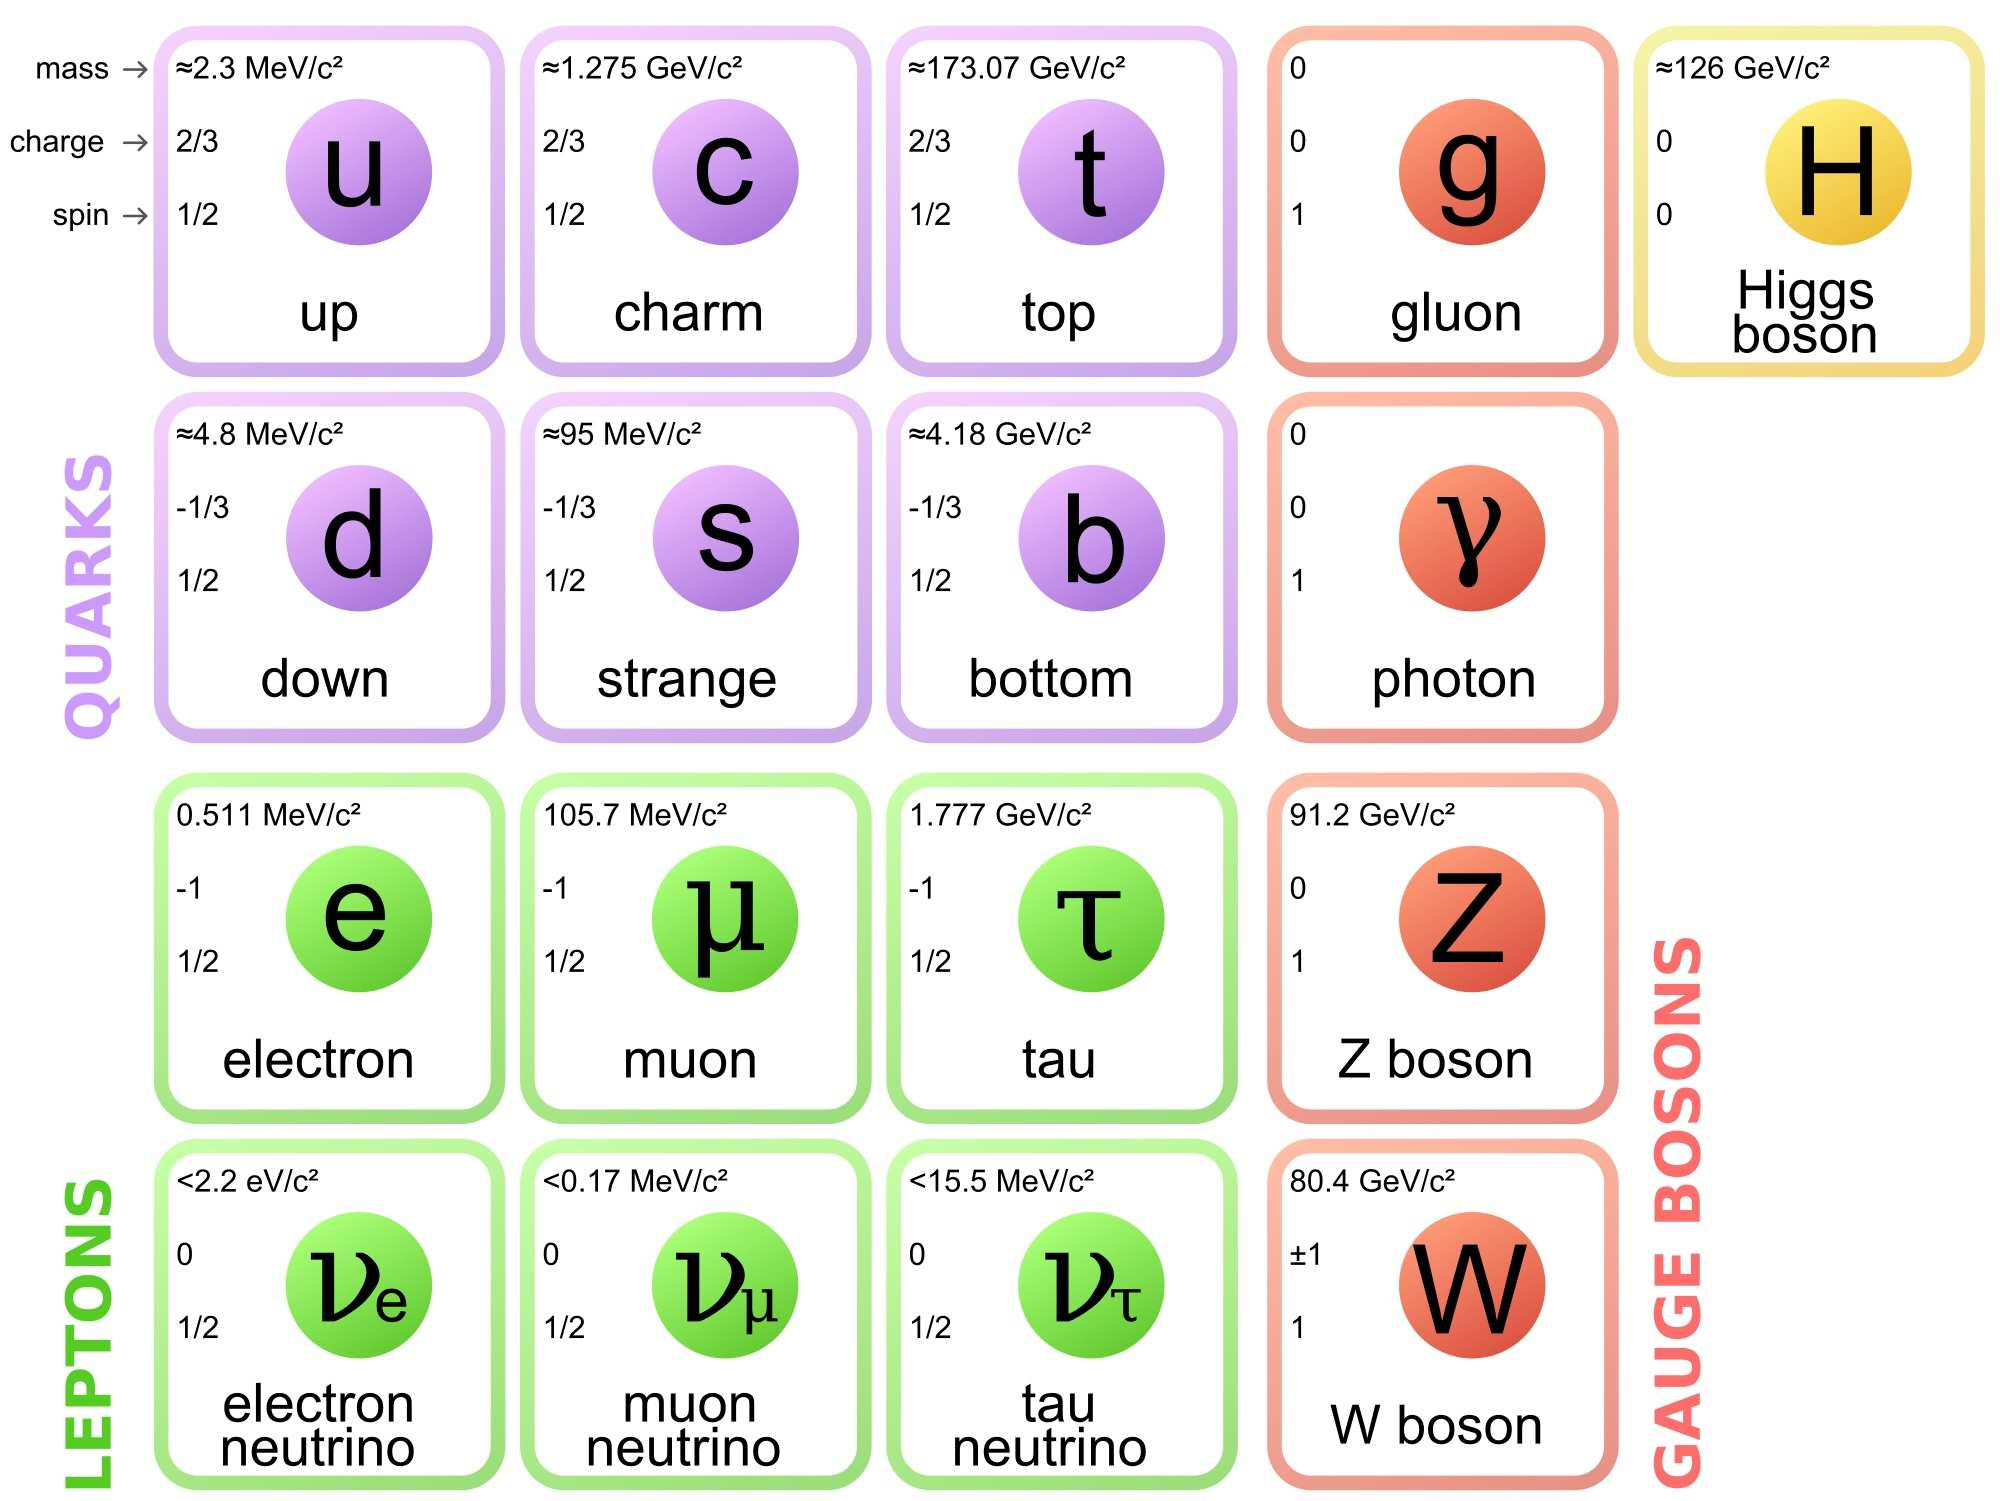
\includegraphics[width=0.9\textwidth,clip] {figures/2000px-Standard_Model_of_Elementary_Particles.png}
\caption{Particle content of the Standard Model.}
\label{fig:standardmodel}
\end{figure}

\subsection{Forces and Symmetries}

% Fundamental interactions in quantum field theory arise from the exchange of gauge bosons, which mediate the four fundamental forces at work in the universe: the strong force, the weak force, the electromagnetic force, and the gravitational force. They work over different ranges and have different strengths: gravity is the weakest but it has an infinite range; the electromagnetic force also has infinite range but it is many times stronger than gravity; the weak and strong forces are effective only over a very short range and dominate at the level of subatomic particles. Despite its name, the weak force is actually much stronger than gravity, though it is indeed the weakest of the other three. The strong force, as the name suggests, is the strongest of all four fundamental interactions.

Fundamental interactions in quantum field theory arise from the exchange of gauge bosons, which mediate three of the fundamental forces at work in the universe: the strong force, the weak force, and the electromagnetic force. They work over different ranges and have different strengths: the electromagnetic force has infinite range and can predominantly drive interactions at intermediate scales; the weak and strong forces are effective only over a very short range and dominate at the level of subatomic particles. The weak force is so named because it is the weakest of the three forces at the scale of partons like quarks. The strong force, as the name suggests, is the strongest of all fundamental interactions between elementary particles at similar scale. 

The strong nuclear force is mediated by gluons, which carry the force that binds quarks together to form protons, neutrons, and other hadrons. Unlike other force carriers, gluons themselves possess color charge, allowing them to interact with one another. At nuclear scales (approximately 1–3 femtometers), a residual effect of this fundamental force termed the ``nuclear force,'' carried by mesons such as pions, binds protons and neutrons together to form atomic nuclei. 

The electromagnetic force, responsible for interactions between electrically charged particles, is mediated by photons. This force contributes to macroscopic interactions at various scales, from atomic bonding to planetary motion (although larger scales are dominated by gravity), and has an infinite range, diminishing in strength with the inverse square of the distance. The electromagnetic force is vastly stronger than gravity but is often neutralized at larger scales due to the balance of positive and negative charges in matter.  

The weak interaction, mediated by the W and Z bosons, governs processes such as beta decay, or neutrino interactions. %, and other flavor-changing reactions. 
The W bosons facilitate charged-current interactions, enabling quarks to change flavor (e.g., converting a neutron into a proton in beta decay) or transforming a lepton into its corresponding neutrino. The Z boson mediates neutral-current interactions, which do not change particle identities but influence their scattering behavior. Unlike the strong and electromagnetic forces, the weak force has a highly limited range ($10^{-18}$ meters), due to the large masses of the W and Z bosons, which restrict their influence.  

% Quarks are held together by gluons, which provide protons and neutrons mass. Quarks can shoot off gluons, since gluons are the mediators of the strong force. The strong interaction is observable at two ranges and mediated by two force carriers. On a larger scale (about 1 to 3 fm), it is the force (carried by mesons like pion which can change neutron to proton and vice versa) that binds protons and neutrons (nucleons) together to form the nucleus of an atom. On the smaller scale (less than about 0.8 fm, the radius of a nucleon), it is the force (carried by gluons) that holds quarks together to form protons, neutrons, and other hadron particles.

% Electrically charged particles can emit photons, which are the mediators of the electromagnetic force.

% Quarks, leptons, and neutrinos can emit Z and W bosons, as mediators of the weak force. W bosons deal with charged-current interactions and are responsible for beta decay (by changing the flavor of a quark in a proton, for example, turning it into a neutron, and then decaying to a positron and electron neutrino) or for turning a lepton into its neutrino (weak isospin differs by 1). Z bosons deal with neutral-current interactions and is responsible for deflection/elastic collisions.

%====================================================================================================

% The weak force is essentially as strong as the electromagnetic force, but it appears weak because its influence is limited by the large mass of the Z and W bosons. Their mass limits the range of the weak force to about 10-18 metres, and it vanishes altogether beyond the radius of a single proton.

% Three of the fundamental forces result from the exchange of force-carrier particles, which belong to a broader group called “bosons”. Particles of matter transfer discrete amounts of energy by exchanging bosons with each other. The strong force is carried by the “gluon”, the electromagnetic force is carried by the “photon”, and the “W and Z bosons” are responsible for the weak force.

% But why are the nuclear forces not long-range forces? 
% Goldstone proved that you can break symmetries by putting a field in empty space. But then even if you give masses to the gauge bosons, you get massless Goldstone bosons. 
% Goldstone's theorem seemed to imply that if you had a symmetry in some form, you would always end up with a massless particle. 
% Thus it was thought that the nuclear forces could not be Yang-Mills theories (based on gauge symmetries) because that would necessarily lead to massless particles, which were definitely not observed in laboratory settings. 

% However, this logic was flawed. In the case of the strong nuclear force, gluons interact with each other. 
% Photons of electromagnetism interact with electrically charged particles, but the photons themselves are not electrically charged.
% However, gluons interact with colored particles, such as quarks, while also being colored themselves. This means that gluons inside nuclei are interacting with each other and this leads to a phenomenon called ``confinement.'' 
% From outside the proton, there’s almost no evidence of the strong nuclear force, but inside a proton it is very strong.

% A different mechanism makes the weak nuclear force short range. 
% The Higgs field fills space and absorbs the weak nuclear force, giving mass to the W and Z bosons.

% The weak nuclear force, while comparable in intrinsic coupling strength to the electromagnetic interaction, appears much weaker at macroscopic scales due to the large mass of its mediating gauge bosons, the W and Z. Unlike the photon, which is massless and therefore allows electromagnetic forces to propagate over infinite distances, the W and Z bosons have masses on the order of 80 and 90 GeV, respectively. This mass constrains the weak interaction to a characteristic range of approximately $10^{-18}$ meters, comparable to the spatial extent of a nucleon. At distances beyond this range, the weak force is exponentially suppressed, effectively vanishing at scales larger than the atomic nucleus.

% Fundamental interactions in quantum field theory arise from the exchange of gauge bosons, which mediate forces between elementary particles. The electromagnetic force is governed by the exchange of photons, which couple to electrically charged particles, while the strong nuclear force is mediated by gluons, which interact with quarks and with each other due to their color charge. The weak interaction, responsible for flavor-changing processes such as beta decay, is carried by the massive W and Z bosons. The key difference between these interactions lies in the properties of their force carriers: the photon and gluons are massless, allowing their respective forces to operate over long or effectively infinite distances, whereas the W and Z bosons acquire mass through the Higgs mechanism, thereby restricting the weak force to subnuclear scales.

A fundamental question in early quantum field theory was why the strong and weak interactions are not long-range, and why there exists only a residual nuclear force outside the proton. Goldstone’s theorem, a critical result in quantum field theory, originally suggested that any spontaneously broken continuous symmetry would necessarily yield massless scalar bosons. This posed a major theoretical challenge, as no such massless particles were observed in experiments involving the weak force. It was thus believed that Yang-Mills gauge theories, which rely on local symmetries, could not correctly describe the weak interaction, since they would seemingly predict unobserved massless bosons.

However, this reasoning was incomplete. In the case of the strong interaction, the resolution lies in the non-abelian nature of quantum chromodynamics (QCD). Unlike electromagnetism, where photons interact with charged particles but remain neutral themselves, gluons possess color charge and therefore interact not only with quarks but also with each other. This self-interaction of gluons inside nuclei gives rise to ``confinement:'' quarks and gluons are permanently bound within hadrons such as protons and neutrons, and the strong force does not manifest significantly beyond nucleonic scales. While the strong force is immensely powerful at short distances, its effects are effectively screened at larger distances and from outside the proton, there’s almost no evidence of the strong force.

However, a completely different mechanism is responsible for the short range of the weak force. It turns out that the Higgs field, which permeates all of space, undergoes spontaneous symmetry breaking, providing a mass mechanism for the weak gauge bosons. In the SM, the electroweak symmetry group $SU(2)_L \times U(1)_Y$ is spontaneously broken to the electromagnetic subgroup $U(1)_{\text{EM}}$ by the Higgs vacuum expectation value, or VEV. This breaking mechanism gives mass to the W and Z bosons while leaving the photon massless, thereby allowing electromagnetism to remain long-range while restricting the weak force to subatomic scales. Despite the weak interaction's intrinsic coupling strength, the large masses of its mediators ensure that weak processes occur only over extremely short distances, making the weak force appear weak at macroscopic scales.

%====================================================================================================

% Philip Anderson in 1963 (Plasmons, Gauge Invariance, and Mass) proposed a field filling space that could give weak interaction bosons a mass and explain why they were not long range.
% Then in 1964 (Broken Symmetry and the Mass of Gauge Vector Mesons), physicists Francois Englert and Robert Brout proposed the idea that is now called the Higgs mechanism.

% Also 1964, ``Broken Symmetries and the Masses of Gauge Bosons'' by Peter Higgs, and ``Global Conservation Laws and Massless Particles'' by Gerald Guralnik, Carl Hagen, and Tom Kibble.

% In 1967 (A Model of Leptons), Steven Weinberg wrote a paper that took the idea of the Higgs mechanism and showed how it explained the weak interactions. Weinberg took Glashow’s model--with enough symmetry to give you the W bosons, the Z boson, and the photon--and used the Higgs field to break those symmetries.

% Similar proposal of Glashow’s model by another physicist named Abdus Salam. Nobel for the electroweak theory was shared by Glashow, Weinberg, and Salam.

% 1971 ``Renormalization of massless Yang-Mills fields'' and ``Renormalizable Lagrangians for massive Yang-Mills fields'' by Gerard 't Hooft.

% The ``ABEGHHK’tH'' boson in stead of the ``Higgs'' boson. 

% The Higgs field permeates all of space and plays a crucial role in electroweak symmetry breaking, providing mass to the weak interaction bosons while leaving the photon massless. This mechanism is fundamental to the Standard Model, explaining why the weak nuclear force operates over a short range while the electromagnetic force remains long-ranged. The theoretical formulation of this idea emerged gradually over several decades, incorporating insights from multiple physicists and culminating in the eventual discovery of the Higgs boson in 2012.


\section{The Higgs Mechanism}

The origins of the Higgs mechanism can actually be traced to condensed matter physics, where Philip Anderson, in his 1963 paper on gauge invariance in superconductors, suggested that a field permeating space could confer mass to otherwise massless gauge bosons. This idea laid the groundwork for the development of a relativistic field-theoretic framework that could explain the mass of weak interaction bosons.

In 1964, several independent groups formalized this concept within the context of particle physics. François Englert and Robert Brout first published a paper describing spontaneous symmetry breaking in gauge theories, demonstrating how vector bosons could acquire mass without violating gauge invariance. Shortly thereafter, Peter Higgs elaborated on this mechanism and explicitly predicted the existence of a new scalar boson, now known as the Higgs boson. Around the same time, Gerald Guralnik, Carl Hagen, and Tom Kibble presented an alternative but equivalent formulation of the same underlying physics. This collective work established what is now recognized as the Higgs mechanism.

In 1967, Steven Weinberg incorporated the Higgs mechanism into electroweak theory, building upon Sheldon Glashow’s earlier work. Glashow had introduced a unified framework for the weak and electromagnetic interactions, postulating the existence of the W and Z bosons along with the photon. However, his model required a mechanism to break symmetry while preserving gauge invariance. Weinberg demonstrated that the Higgs field could accomplish this, allowing for the spontaneous breaking of electroweak symmetry and thereby endowing the W and Z bosons with mass while keeping the photon massless. Around the same time, Abdus Salam independently developed a similar theory. The electroweak theory, formulated by Glashow, Weinberg, and Salam, was instrumental in shaping the SM and earned the three physicists the 1979 Nobel Prize in Physics.

A major hurdle for early versions of the electroweak theory was the question of renormalizability—whether the theory could yield finite, predictive results at all energy scales. In 1971, Gerard ’t Hooft, under the supervision of Martinus Veltman, demonstrated that gauge theories with spontaneously broken symmetry, including the electroweak theory, were renormalizable. This work provided the final theoretical validation of the SM framework and solidified the Higgs mechanism as a cornerstone of modern particle physics.

Although widely referred to as the Higgs boson, some physicists have suggested that its name should reflect the collective contributions of multiple researchers. The term ``ABEGHHK’tH boson'' has been proposed, incorporating the initials of Anderson, Brout, Englert, Guralnik, Hagen, Higgs, Kibble, and ’t Hooft. However, historical convention has cemented the use of “Higgs boson” in both scientific and popular discourse.

%====================================================================================================

% The Higgs boson is not a gauge boson. In particular, the spin of the Higgs is zero, making it a scalar. This scalar boson is associated with the Higgs field, a scalar field that permeates all of space. Mathematically, the Higgs field $\phi$ is a complex scalar field with four degrees of freedom:
% \[
% \phi = \begin{pmatrix} \phi^+ \\ \phi^0 \end{pmatrix}.
% \]

% The field undergoes a spontaneous symmetry breaking due to the potential:
% \[
% V(\phi) = \mu^2|\phi|^2 + \lambda|\phi|^4,
% \]
% where $\mu^2 < 0$ and $\lambda > 0$. The negative mass term ($\mu^2 < 0$) causes the field to acquire a nonzero vacuum expectation value (VEV):
% \[
% \langle \phi \rangle = \begin{pmatrix} 0 \\ v/\sqrt{2} \end{pmatrix},
% \]
% where $v \approx 246\,\mathrm{GeV}$ is the VEV.




% The Higgs mechanism is the process by which gauge bosons in a spontaneously broken gauge theory acquire mass while maintaining gauge invariance. This mechanism is fundamental to the Standard Model (SM), where it explains the masses of the \( W \) and \( Z \) bosons and plays a crucial role in electroweak symmetry breaking (EWSB). Below, we outline the key mathematical aspects of the Higgs mechanism, including the Higgs scalar field, its potential, the vacuum expectation value (VEV), and how mass terms emerge for both vector bosons and fermions.

%====================================================================================================



In today's SM, the Higgs field is introduced as a complex scalar doublet under the electroweak gauge group \( SU(2)_L \times U(1)_Y \):

\begin{equation}
\label{eq:higgscalar}
    \Phi = \begin{pmatrix} \phi^+ \\ \phi^0 \end{pmatrix},
\end{equation}

where \( \phi^+ \) and \( \phi^0 \) are complex scalar fields. This field transforms under \( SU(2)_L \times U(1)_Y \) as \(\Phi \to e^{i\alpha^a \tau^a} e^{i\beta Y} \Phi,\) where \( \tau^a \) are the generators of \( SU(2) \), and \( Y \) is the hypercharge.

The dynamics of the Higgs field are governed by the Higgs potential:

\begin{equation}
\label{eq:higgpot}
V(\Phi) = \mu^2 \Phi^\dagger \Phi + \lambda (\Phi^\dagger \Phi)^2.
\end{equation}

The form of this potential depends on the sign of \( \mu^2 \). If \( \mu^2 > 0 \), the minimum of \( V(\Phi) \) occurs at \( \Phi = 0 \), preserving the full electroweak symmetry. If \( \mu^2 < 0 \), the potential acquires a ``Mexican hat'' shape, leading to spontaneous symmetry breaking (SSB) as illustrated in Figure~\ref{fig:mexicanhat}.

\begin{figure}[h!]
  \centering
  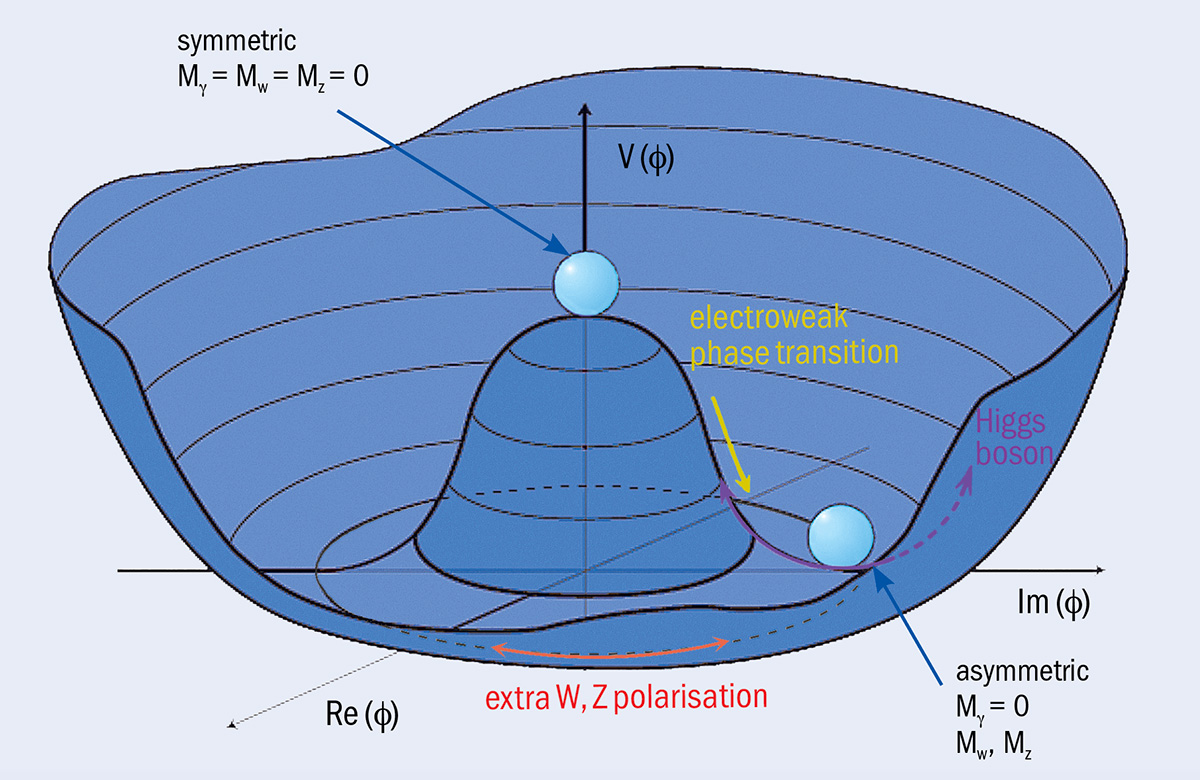
\includegraphics[width=0.8\textwidth,clip] {figures/CERNliftinglid.jpg}
  \caption{Visualization of the characteristic ``Mexican hat'' shaped potential~\cite{Thethril79:online}.}
  \label{fig:mexicanhat}
\end{figure}

For \( \mu^2 < 0 \), the Higgs field acquires a vacuum expectation value (VEV), breaking the electroweak symmetry:

\begin{equation}
\label{eq:higgssymmetry}
\langle \Phi \rangle = \frac{1}{\sqrt{2}} \begin{pmatrix} 0 \\ v \end{pmatrix}.
\end{equation}

Here, \( v \) is determined by minimizing the potential\footnote{Experimentally, the VEV is found to be approximately \( v \approx 246 \) GeV.}:

\begin{equation}
\label{eq:higgspotmin}
v = \sqrt{\frac{-\mu^2}{\lambda}}.
\end{equation}

The Higgs field interacts with the electroweak gauge bosons via the covariant derivative:

\begin{equation}
\label{eq:higgscovder}
D_\mu \Phi = \left( \partial_\mu - i g W^a_\mu \tau^a - i g' B_\mu Y \right) \Phi.
\end{equation}

Expanding around the VEV and extracting the quadratic terms in the Lagrangian, the mass terms for the gauge bosons emerge. The kinetic term for the Higgs field, 

\begin{equation}
\label{eq:higgskinetic}
(D_\mu \Phi)^\dagger (D^\mu \Phi),
\end{equation}

yields mass terms for the weak bosons:

\begin{equation}
\label{eq:higgsweakmass}
M_W = \frac{1}{2} g v, \quad M_Z = \frac{1}{2} \sqrt{g^2 + g'^2} v.
\end{equation}

The photon remains massless, as expected, since the Higgs mechanism only breaks \( SU(2)_L \times U(1)_Y \) down to \( U(1)_{\text{EM}} \).

Fermion masses arise through Yukawa interactions of the Higgs field with the fermion fields. The Yukawa coupling takes the form:

\begin{equation}
\label{eq:higgsyukawa}
\mathcal{L}_Y = - y_f \bar{\psi}_L \Phi \psi_R + \text{h.c.}
\end{equation}

After the Higgs field acquires a VEV, this interaction produces mass terms proportional to each fermion's Yukawa coupling strength \( y_f \):

\begin{equation}
\label{eq:higgsfermmass}
M_f = \frac{y_f v}{\sqrt{2}}.
\end{equation}

Thus, the Higgs mechanism provides a consistent and gauge-invariant way for the weak bosons and fermions to acquire mass while preserving renormalizability. The Higgs scalar field, through its spontaneous symmetry breaking, generates mass terms for the \( W \) and \( Z \) bosons, while fermions gain mass through Yukawa interactions. 

% The discovery of the Higgs boson at the LHC confirmed the validity of this mechanism and solidified the Standard Model's foundation, though open questions remain regarding the nature of electroweak symmetry breaking and possible physics beyond the Standard Model.

%====================================================================================================



% Through the Higgs mechanism, the interaction of particles with the Higgs field gives rise to their masses. Gauge bosons, such as the $W$ and $Z$ bosons, acquire masses proportional to $v$, while the photon remains massless. Fermions gain mass via Yukawa interactions:
% \[
% \mathcal{L}_\text{Yukawa} = -y \bar{\psi} \phi \psi ,
% \]
% where $y_f$ is the Yukawa coupling for a fermion $f$. The masses of fermions are proportional to $y_f v$.



%====================================================================================================
% HIGGS COCKTAIL PARTY ANALOGY
%====================================================================================================


% \begin{figure}[h!]
% \centering
% 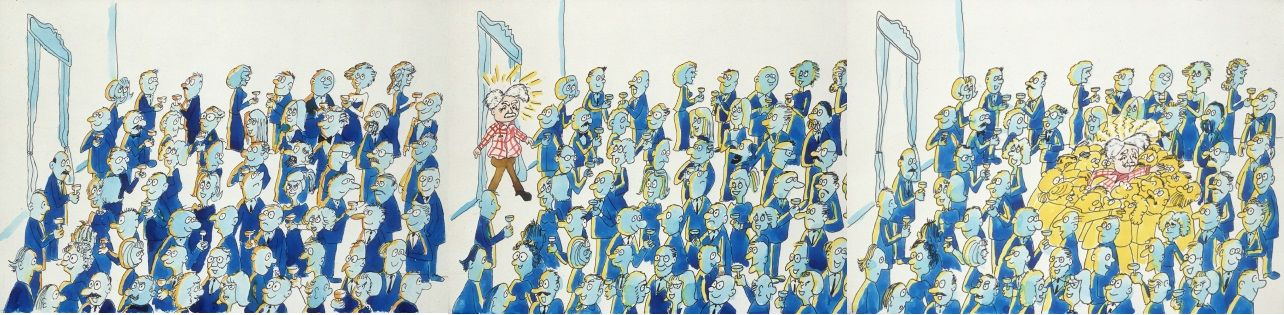
\includegraphics[width=0.9\textwidth,clip] {figures/famousphysicist.jpg}
% \caption{}
% \label{fig:famousphysicist}
% \end{figure}


% \begin{figure}[h!]
% \centering
% 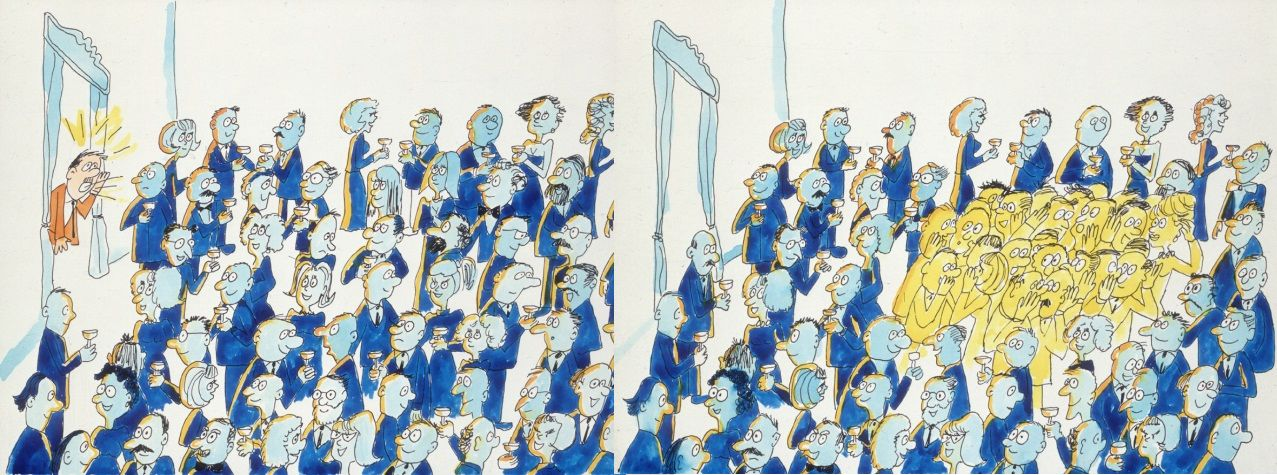
\includegraphics[width=0.9\textwidth,clip] {figures/gossip.jpg}
% \caption{}
% \label{fig:gossip}
% \end{figure}



%====================================================================================================


For decades, the Higgs boson remained the final missing piece of the SM. Its discovery required a collider capable of reaching energy scales high enough to produce it. This challenge was met by the Large Hadron Collider (LHC) at CERN, where the ATLAS and CMS experiments, in 2012, independently observed a particle consistent with the predicted properties of the Higgs boson. This landmark discovery confirmed the Higgs mechanism and earned François Englert and Peter Higgs the 2013 Nobel Prize in Physics.

While the Higgs boson’s discovery marked a triumph for the SM, it also highlighted unresolved mysteries in fundamental physics. Among the persistent shortcomings of the SM, we note that there is no inclusion of a force carrier for gravity, or so-called ``graviton.'' Furthermore, the SM still does not contain any description of dark matter, which seems to outweigh visible matter roughly six to one. Or any explanation for the matter-antimatter asymmetry that we observe in our universe, despite the fact that, in principle, particles formed in the early universe should have had an equal chance of becoming matter or antimatter.
%~\cite{Darkmatt18}%~\cite{Thematte44}

Answers to these questions, or at least hints to guide our way, hinge upon the search for evidence of physics Beyond the Standard Model (BSM). Given the extraordinary success of the SM in describing the known fundamental particles and their interactions, any necessary modifications or extensions to this framework are most effectively probed through the observation of subtle anomalies, discrepancies between theoretical expectations and precision measurements. The Higgs boson offers a natural point of connection to potential new physics, particularly in the context of dark matter\footnote{Unlike SM particles, dark matter remains elusive, with its non-gravitational interactions yet to be directly detected.}. Since dark matter must possess mass, it is plausible that dark matter particles couple to the Higgs boson.
%~\cite{CERNandt20}

If dark matter (or any other anomalous particle) does indeed couple to the Higgs field, then precise measurements of Higgs boson production and decay processes could reveal subtle anomalies—shifts in branching ratios, invisible decays, or unexpected interaction strengths—that point toward the existence of new, BSM particles. Thus, studying the Higgs boson in unprecedented detail represents one of our most promising strategies for uncovering the true nature of dark matter and extending our understanding of fundamental physics beyond the SM.



% Answers to these questions or at least hints to guide our way, we expect to find through evidence of BSM (Beyond the Standard Model) physics. Necessary changes or extensions to the SM framework are likely best probed through the observation of anomalous behavior, or physics that does not exactly match our Standard Model predictions. And with the (relatively) recent experimental confirmation of the Higgs boson, we now have a promising window through which we can search for such anomalous behavior. Because of the role that the Higgs field plays in giving mass to particles through the Brout-Englert-Higgs mechanism, it is reasonable to expect dark matter particles to exhibit some coupling to the Higgs boson~\cite{CERNandt20}. In fact, because dark matter seems to strictly interact with observable matter through gravitational effects, probing at the mechanism which gives it mass may be our best way to learn more about its characteristics.


% Extensions of the Standard Model, such as supersymmetry and grand unified theories, propose new particles and interactions that could address these open questions. Experimental searches at high-energy colliders, neutrino observatories, and astrophysical experiments continue to probe these mysteries, potentially paving the way for the next major breakthrough in our understanding of fundamental physics.

% The Higgs mechanism, once a theoretical curiosity, has become a central pillar of modern physics. From its conceptual origins in superconductivity to its incorporation into the electroweak theory and its experimental confirmation, the Higgs field has reshaped our understanding of mass, symmetry breaking, and fundamental forces. Yet, despite its success, many questions remain unanswered, ensuring that the quest for deeper insights into the nature of the universe continues.

%====================================================================================================

% The Standard Model includes 4 force carriers: the gluon, photon, Z boson, and W boson. These mediate the strong, electromagnetic, and weak forces respectively. The discovery of the Higgs boson in 2012 at the Large Hadron Collider (LHC) added a significant contribution to this picture of our physical understanding, via an experimentally confirmed Higgs field with which various elementary particles can interact to acquire mass. 

% Among the persistent shortcomings of the Standard Model, we note that there is no inclusion of a force carrier for gravity, or so-called ``graviton.'' Furthermore, the Standard Model still does not contain any description of dark matter, which seems to outweigh visible matter roughly six to one~\cite{Darkmatt18}. Or any way to explain the matter/antimatter asymmetry that we observe in our universe where matter is abundant, despite the fact that in principle, after the Big Bang, particles formed in the early universe should have had an equal chance of becoming matter or antimatter~\cite{Thematte44}.

% Answers to these questions or at least hints to guide our way, we expect to find through evidence of BSM (Beyond the Standard Model) physics, essentially extensions to our current Standard Model. While it is possible that our description of elementary physics will require an overhaul in the future, the consistent reliability of the Standard Model provides a promising starting point and very accurate physical description at the energies that we can experimentally observe as a species.

% Such necessary changes to the SM framework are likely best probed through the observation of anomalous behavior, or physics that does not exactly match our Standard Model predictions. And with the (relatively) recent experimental confirmation of the Higgs boson, we now have a promising window through which we can search for such anomalous behavior. Because of the role that the Higgs field plays in giving mass to particles through the Brout-Englert-Higgs mechanism, it is reasonable to expect dark matter particles to exhibit some coupling to the Higgs boson~\cite{CERNandt20}. In fact, because dark matter seems to strictly interact with observable matter through gravitational effects, probing at the mechanism which gives it mass may be our best way to learn more about its characteristics.









\section{Phenomenology of the off-shell Higgs boson}


% % epigraph after chapter heading
% \epigraph{Since it is written in \LaTeX, it must be true.}{-- Isaac Newton}


%%%% MUST: add the citation for the chapter if it is a reprint

% \blindtext\footnote{Hello, this is the first footnote with no indentation and single-spaced text. The spacing between two footnotes is also single-spaced.}

Since 2012, both ATLAS and CMS have observed a Higgs Boson with mass around 125 GeV~\cite{20121}~\cite{201230} which is consistent with our SM expectations. The Higgs boson's mass, as the last free parameter of the SM, is necessarily determined experimentally and is instrumental in our understanding of the SM, along with the Higgs boson's other properties such as its width and couplings to other particles. And as we discussed, precision measurements of the Higgs boson are invaluable in our search for deviations from our SM expectation due to BSM effects.

% For every interaction the Higgs has with a fermion, there’s a unique coupling constant which determines the mass of that particle. But it also helps us calculate the rate of decay of the Higgs into other particles. 

Now, in the SM, ``virtual'' particles can have a mass that is different from the mass that the
particle would have if it were ``real,'' or physical. Inside a Feynman diagram\footnote{Feynman diagrams are pictorial representations of interactions between subatomic particles. They provide an intuitive way to illustrate and organize the many terms which arise in expansions of quantum field theory (QFT) descriptions of such interactions.}, virtual particles can have any mass because these aren’t really particles; they are excitations in quantum fields.
This lets us draw Feynman diagrams with intermediary particles of masses very different from their SM mass. 
We call such particles with masses away from their pole mass ``off-shell.''  The terminology arises from the notion that a particle is produced ``on the mass shell'' when its invariant mass is close to the SM expectation, whereas an ``off-shell'' particle is produced significantly away from this nominal pole mass. This thesis will focus on measurements of the off-shell Higgs boson, for reasons to be presented. 

\subsection{Production Modes}

At collision energies around 13 TeV, we certainly have enough energy to produce the Higgs boson at the LHC, as observed in the plot of proton-proton cross sections in Figure~\ref{fig:prodModes}. Production occurs via four dominant modes which have the Feynman diagrams illustrated in Figure~\ref{fig.Hproduction}. As one can see, each of the dominant production diagrams begin with quarks or gluons from the proton-proton collisions. Our dominant production mode, gluon fusion, can be seen in Figure~\ref{fig.ggH} and at leading order involves a quark loop since the Higgs boson does not couple directly to the massless gluons. The primary contribution is with a loop of top quarks (the heaviest quark), with a small contribution from the bottom quark (the second heaviest). At higher order, radiated gluons and other jets (created through QCD effects from the inital state gluons) can be produced along with the Higgs boson. 

The second most productive mechanism is vector boson fusion (VBF), shown in Figure~\ref{fig.VBF}, in which two vector bosons are radiated from our initial state quarks and then interact to ``fuse'' and generate a Higgs boson. Because the W and Z vector bosons have mass around 80-90 GeV, VBF can involve the radiation of hundreds of GeV especially at higher energies when the vector bosons come on-shell. This means that the two quark jets emitted from a VBF event characteristically possess large transverse energies and are often emitted opposite each other. 

\begin{figure}[!h]
\centering
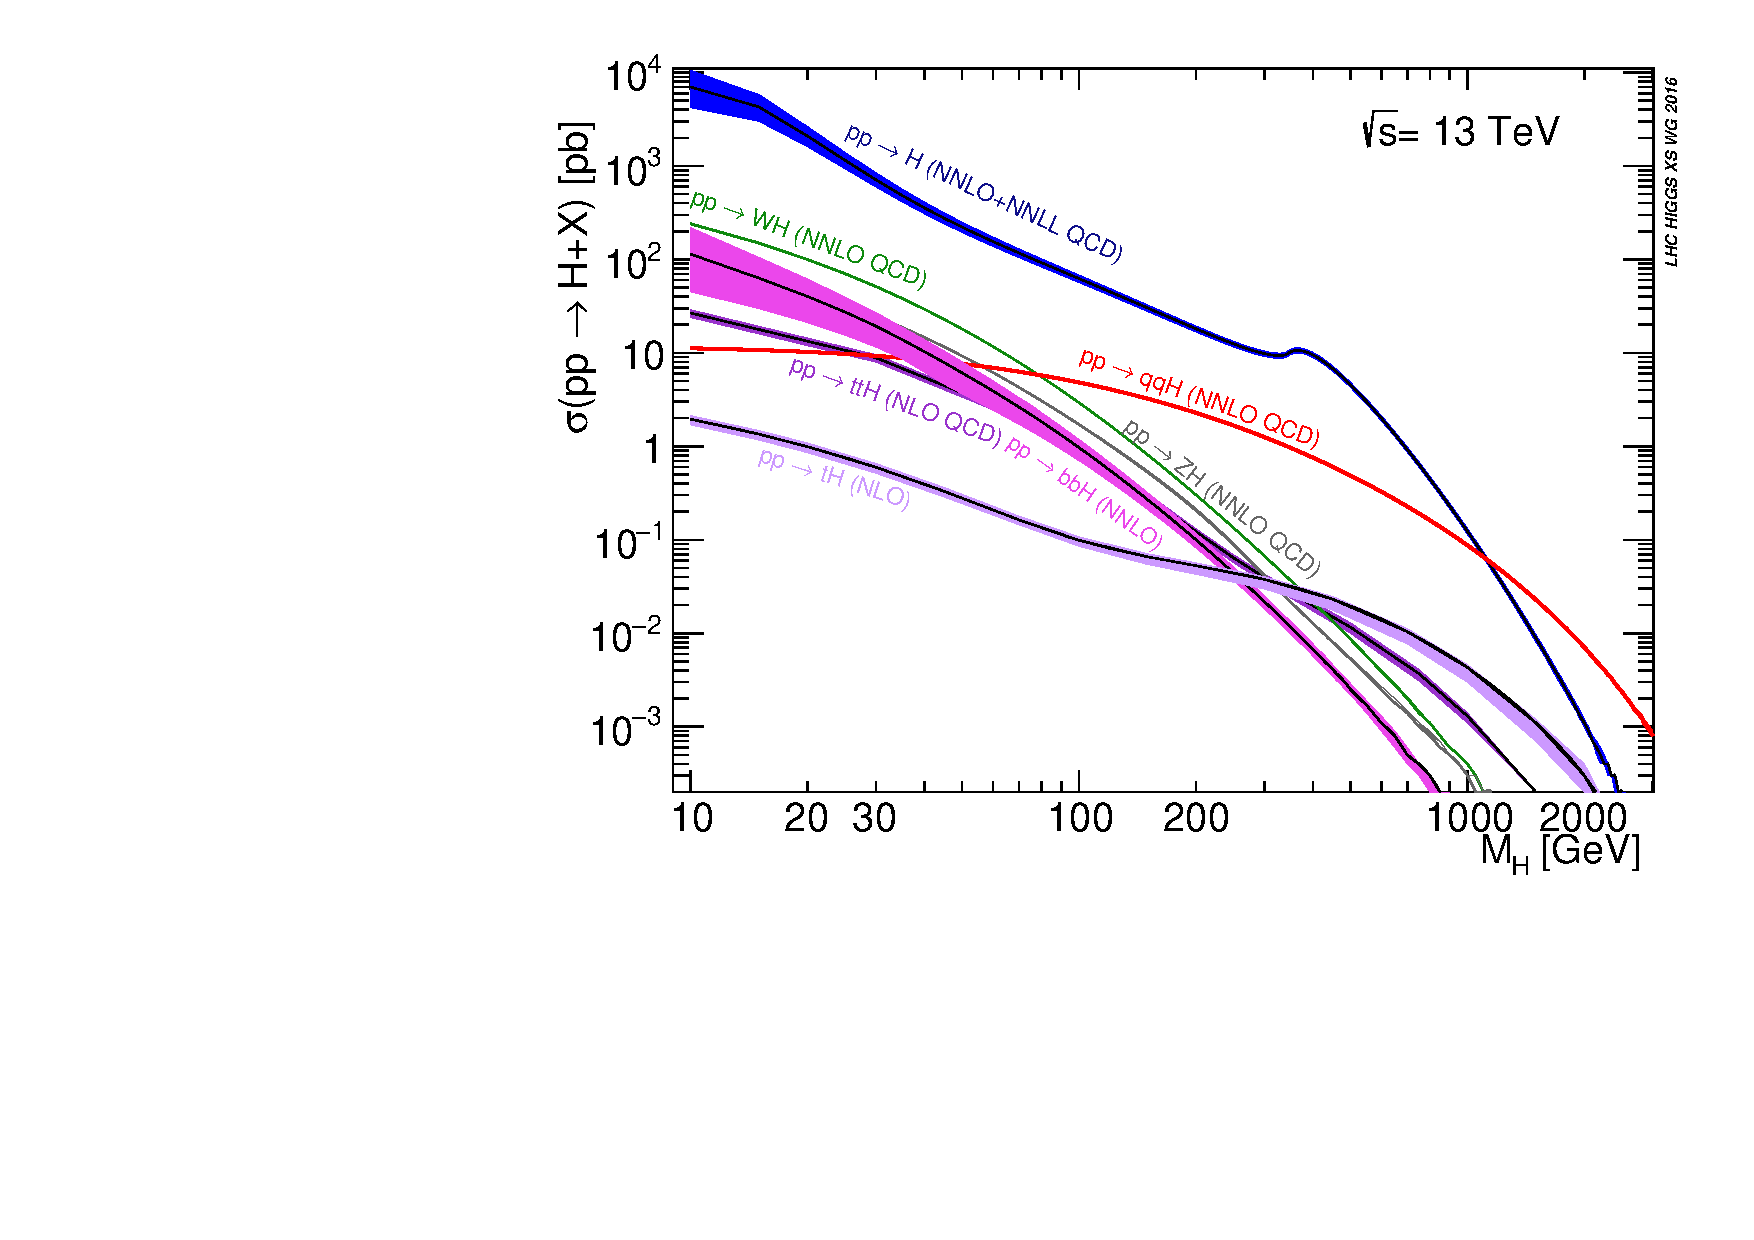
\includegraphics[width=0.9\textwidth,clip] {figures/plotAll_13tev_BSM_sqrt.pdf}
\caption{SM Higgs boson production cross-sections as a function of $m_{H}$ at the LHC at $E_{CM}=13$ TeV~\cite{YR4}.}
\label{fig:prodModes}
\end{figure}

The third most common production mode for both on-shell and off-shell Higgs boson production is associated production with a vector boson, or VH production. This is also known as VH or Higgs-strahlung production, since it closely resembles how a photon can be radiated by an electron through Bremsstrahlung radiation. In VH production, as seen in Figure \ref{fig.VH}, two initial state quarks will produce an energetic vector boson which radiates a Higgs boson. This means that a $q\bar{q}$ initial state results in a VH final state. 

Finally, most of the remaining Higgs boson cross section comes from ttH production, Figure \ref{fig.ttH}. This production mode, along with bbH and other less common mechanisms, becomes less relevant in the production of the off-shell Higgs boson as one can see in Figure \ref{fig:prodModes}. In the off-shell region (chosen to include energies above 180 GeV), the relevant production modes to consider are ggH, VBF, and VH. 

\begin{figure}[!ht]\centering
    \begin{subfigure}{0.45\textwidth}
        \begin{fmffile}{ggH}
          \begin{fmfgraph*}(150,80)
            \fmfstraight
            \fmfleft{i1,i2}
            \fmfright{o1,m,o2}
            % gluons
            \fmf{gluon}{i1,t1}
            \fmf{gluon}{t2,i2}
            \fmf{phantom,tension=0.4}{t1,o1}
            \fmf{phantom,tension=0.4}{t2,o2}
            \fmffreeze
            % top loop
            \fmf{fermion,tension=1}{t1,t2,t3,t1}
            \fmf{phantom,tension=1.4}{t3,m}
            \fmffreeze
            % Higgs boson
            % \fmf{dashes,tension=1.4}{t2,h}
            \fmf{dashes,tension=1.4}{t3,m}
            % \fmf{dashes,tension=1}{h,o2}
            
            % \fmf{dashes,tension=1}{h,o1}
            % \fmf{dashes,tension=1}{h,o2}
          \end{fmfgraph*}
        \end{fmffile}
        \caption{}
        \label{fig.ggH}
    \end{subfigure}
\hfil
    \begin{subfigure}{0.45\textwidth}
        \begin{fmffile}{VBF}
          \begin{fmfgraph*}(150,80)
            \fmfleft{i1,i3} 
            \fmfright{o1,o2,o3}
            \fmf{fermion}{i1,v1,o1}
            \fmf{fermion}{i3,v3,o3}
            \fmf{phantom,tension=0.3}{v1,v3}
            \fmffreeze
            % \fmf{boson,label=$V$,label.side=left}{v3,v2,v1}
            \fmf{boson}{v3,v2,v1}
            \fmf{dashes}{v2,o2}
            % \fmflabel{$q$}{i3}
            % \fmflabel{$q'$}{i1}
            % \fmflabel{H}{o2}
          \end{fmfgraph*}
        \end{fmffile}
        \caption{}
        \label{fig.VBF}
    \end{subfigure}
\hfil
    \begin{subfigure}{0.45\textwidth}
        \begin{fmffile}{VH}
          \begin{fmfgraph*}(150,80)
            \fmfset{wiggly_len}{18}
            \fmfleft{i1,i2}
            \fmfright{o1,o2}
            \fmf{fermion}{i1,v1}
            \fmf{fermion}{i2,v1}
            % \fmf{boson,label=$V^*$,label.side=left}{v1,v2}
            \fmf{boson}{v1,v2}
            % \fmf{boson,label.side=left}{v2,o2}
            \fmf{boson}{v2,o2}
            \fmf{dashes}{v2,o1}
            % \fmflabel{$q'$}{i1}
            % \fmflabel{$q$}{i2}
            % \fmflabel{$V$}{o2}
            % \fmflabel{H}{o1}
          \end{fmfgraph*}
        \end{fmffile}
    \caption{}
    \label{fig.VH}
    \end{subfigure}
\hfil
    \begin{subfigure}{0.45\textwidth}
        \begin{fmffile}{ttH}
          \begin{fmfgraph*}(150,80)
            \fmfleft{d,i1,d,d,i3,d}
            \fmfright{o1,d,o2,d,o3}
            \fmf{gluon,tension=1.2}{i1,v1}
            \fmf{gluon,tension=1.2}{v3,i3}
            \fmf{fermion}{o1,v1}
            \fmf{fermion}{v3,o3}
            \fmf{phantom,tension=0.3}{v1,v3}
            \fmffreeze
            \fmf{fermion}{v1,v2,v3}
            \fmf{dashes,tension=1.3}{v2,o2}
            % \fmflabel{$g$}{i3}
            % \fmflabel{$g$}{i1}
            % \fmflabel{$t$}{o3}
            % \fmflabel{$\bar{t}$}{o1}
            % \fmflabel{H}{o2}
          \end{fmfgraph*}
        \end{fmffile}
    \caption{}
    \label{fig.ttH}
    \end{subfigure}
    \caption{Feynman diagrams for the dominant Higgs boson production modes at the LHC: (a) gluon fusion (ggH), (b) vector boson fusion (VBF), (c) associated (VH) production, and (d) \(t\bar{t}H\) production.}
    \label{fig.Hproduction}
\end{figure}

\subsection{Decay Modes}

% The Higgs boson couples to its decay products based on their masses. At a Higgs mass of 125 GeV or lower, the dominant decay mode is H $\rightarrow$ bb, as b-quarks are the heaviest available decay products. At higher masses, the decays H $\rightarrow$ WW and H $\rightarrow$ ZZ become more prevalent. Relative to the vector boson decays, the channels H $\rightarrow$ $\gamma \gamma$ and H $\rightarrow$ Z$\gamma$ have significantly smaller branching ratios because a massless photon cannot couple directly to the Higgs, and thus requires a loop with massive particles to mediate.

% The sensitivity of a particular decay channel depends on its branching ratio, reconstructed mass resolution, and backgrounds. The H $\rightarrow$ bb channel faces significant QCD background noise and has poor mass resolution. In the H $\rightarrow$ WW channel, missing energy from neutrinos in the final decay products can complicate detection of Higgs events. So, although its expected cross section is smaller compared to H $\rightarrow$ bb or H $\rightarrow$ WW, the H $\rightarrow$ ZZ $\rightarrow$ 4l process has minimal background interference and allows for full decay kinematics with high resolution. This is why the H $\rightarrow$ ZZ $\rightarrow$ 4l is often also referred to as the ``Golden Channel'' and is an ideal channel for both the discovery and measurement of the Higgs boson's properties.

The interaction strength of the Higgs boson with its decay products is directly proportional to their masses. As illustrated in Figure \ref{fig:HiggsDecay}, at a Higgs boson mass around 125 GeV, the dominant decay mode is \( H \to b\bar{b} \), since the bottom quark is the heaviest kinematically accessible fermion. However, as the Higgs boson's mass increases beyond this threshold, decays into electroweak gauge bosons, specifically \( H \to WW \) and \( H \to ZZ \), become dominant due to their larger coupling strength and enhanced phase space availability as there is enough energy for the vector bosons to exist on-shell. The loop-induced processes \( H \to \gamma\gamma \) and \( H \to Z\gamma \) have significantly lower branching fractions, as the Higgs boson does not couple directly to massless photons; these decays proceed via higher-order quantum corrections involving virtual heavy particles in the loop, such as top quarks or \( W \) bosons.

\begin{figure}[!h]
\centering
\begin{subfigure}[t]{0.45\textwidth}
    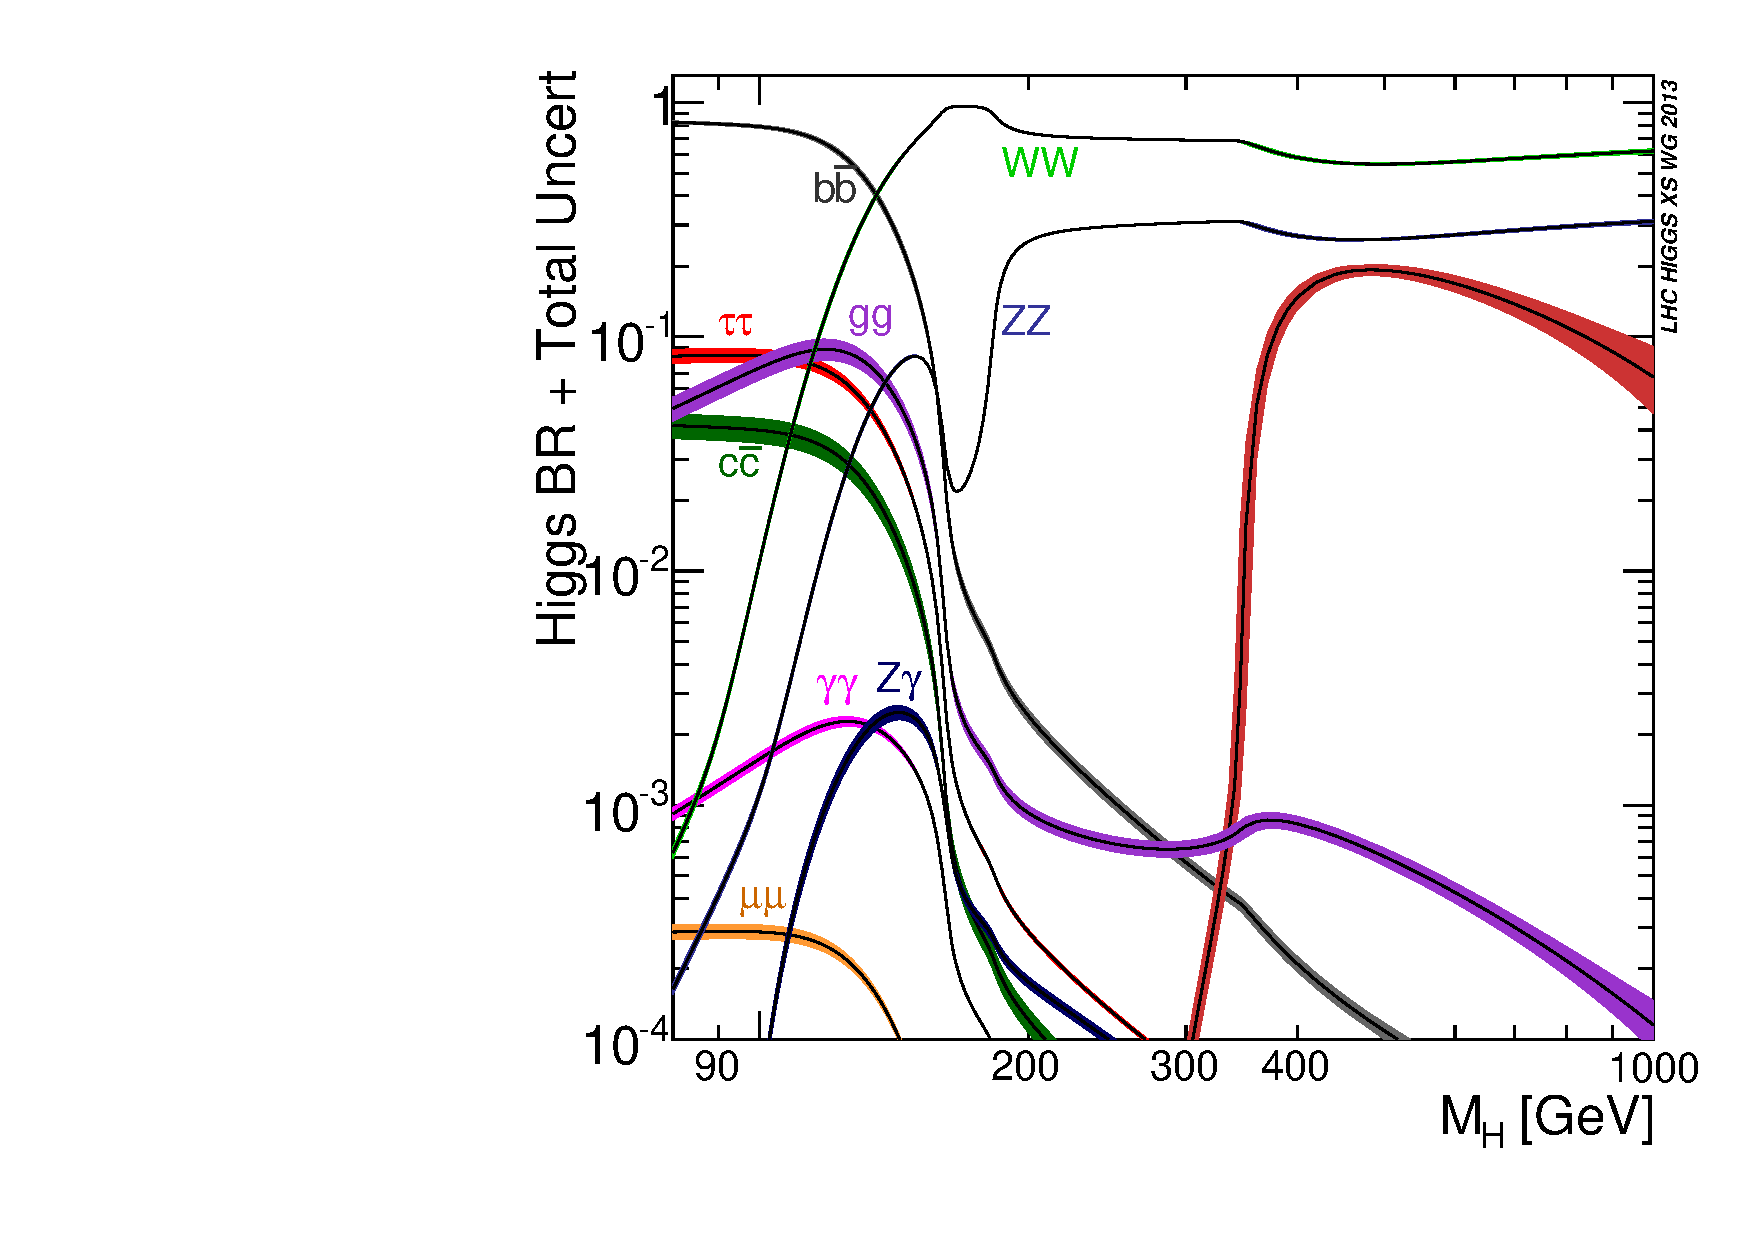
\includegraphics[width=\textwidth]{figures/Higgs_BR.pdf}
    \label{fig:HiggsBR}
\end{subfigure}
\begin{subfigure}[t]{0.45\textwidth}
    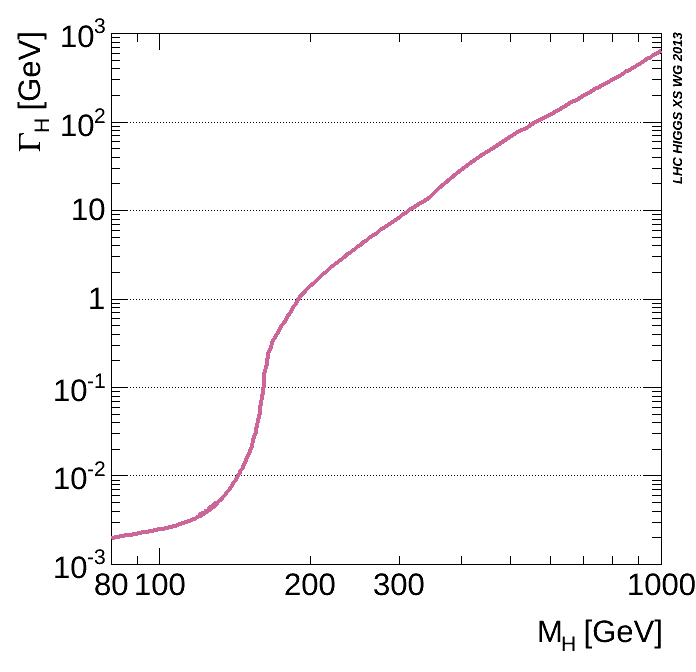
\includegraphics[width=\textwidth]{figures/SM_Width.png}
    \label{fig:SMwidth}
\end{subfigure}
\caption{SM Higgs boson decay branching ratios (left) and total decay width (right) as a function of mass $m_{H}$~\cite{YR4}. In the off-shell region above 180 GeV, the Higgs boson decay to a pair of vector bosons dominates. We see an enhancement of the Higgs boson width at energies above $2m_V$ when the two vector bosons become on-shell.}
\end{figure}
\label{fig:HiggsDecay}

The experimental sensitivity of a given decay channel is determined not only by the branching fraction but also by factors such as the mass resolution of reconstructed final states and the level of irreducible and reducible backgrounds. The \( H \to b\bar{b} \) channel, despite its large branching ratio, suffers from overwhelming quantum chromodynamic (QCD) backgrounds and poor mass resolution, making precise measurements challenging. The \( H \to WW \) decay, while more distinctive, involves final-state neutrinos that escape detection, leading to missing transverse energy and complications in fully reconstructing the Higgs boson's invariant mass.

% The \( H \to ZZ \) channel, although having a smaller overall production cross-section compared to \( H \to b\bar{b} \) or \( H \to WW \), 
The \( H \to ZZ \) channel provides a particularly clean final state, especially in the fully leptonic decay mode \( H \to ZZ \to 4\ell \) (where \( \ell = e, \mu \)). This process benefits from a low background contamination, fully reconstructible decay products, and excellent mass resolution, making it an optimal channel for precision measurements of the Higgs boson properties. As a result, this thesis will primarily focus on the \( H \to ZZ \) decay mode for detailed studies of the Higgs boson.

\begin{figure}[!h]\centering
    \begin{fmffile}{decay}
      \begin{fmfgraph}(150,150)
        \fmfstraight
        \fmfleft{i0,i1,i2}
        \fmfright{o1,o2,o3,o4}
        % fermions
        \fmf{fermion}{o1,v21,o2}
        \fmf{fermion}{o3,v22,o4}
        % phantoms to pull back fermion lines
        \fmf{phantom}{i0,v21}
        \fmf{phantom,tension=0.5}{v21,v22}
        \fmf{phantom}{i2,v22}
        \fmffreeze
        % HWW
        \fmf{dashes,tension=1.5}{i1,v1}
        \fmf{boson}{v1,v21}
        \fmf{boson}{v1,v22}
      \end{fmfgraph}
    \end{fmffile}
    \caption{Feynman diagram for the decay of a Higgs boson to two vector bosons and four leptons.}
    \label{fig.Hdecay}
\end{figure}





% \begin{figure}
% \centering
% 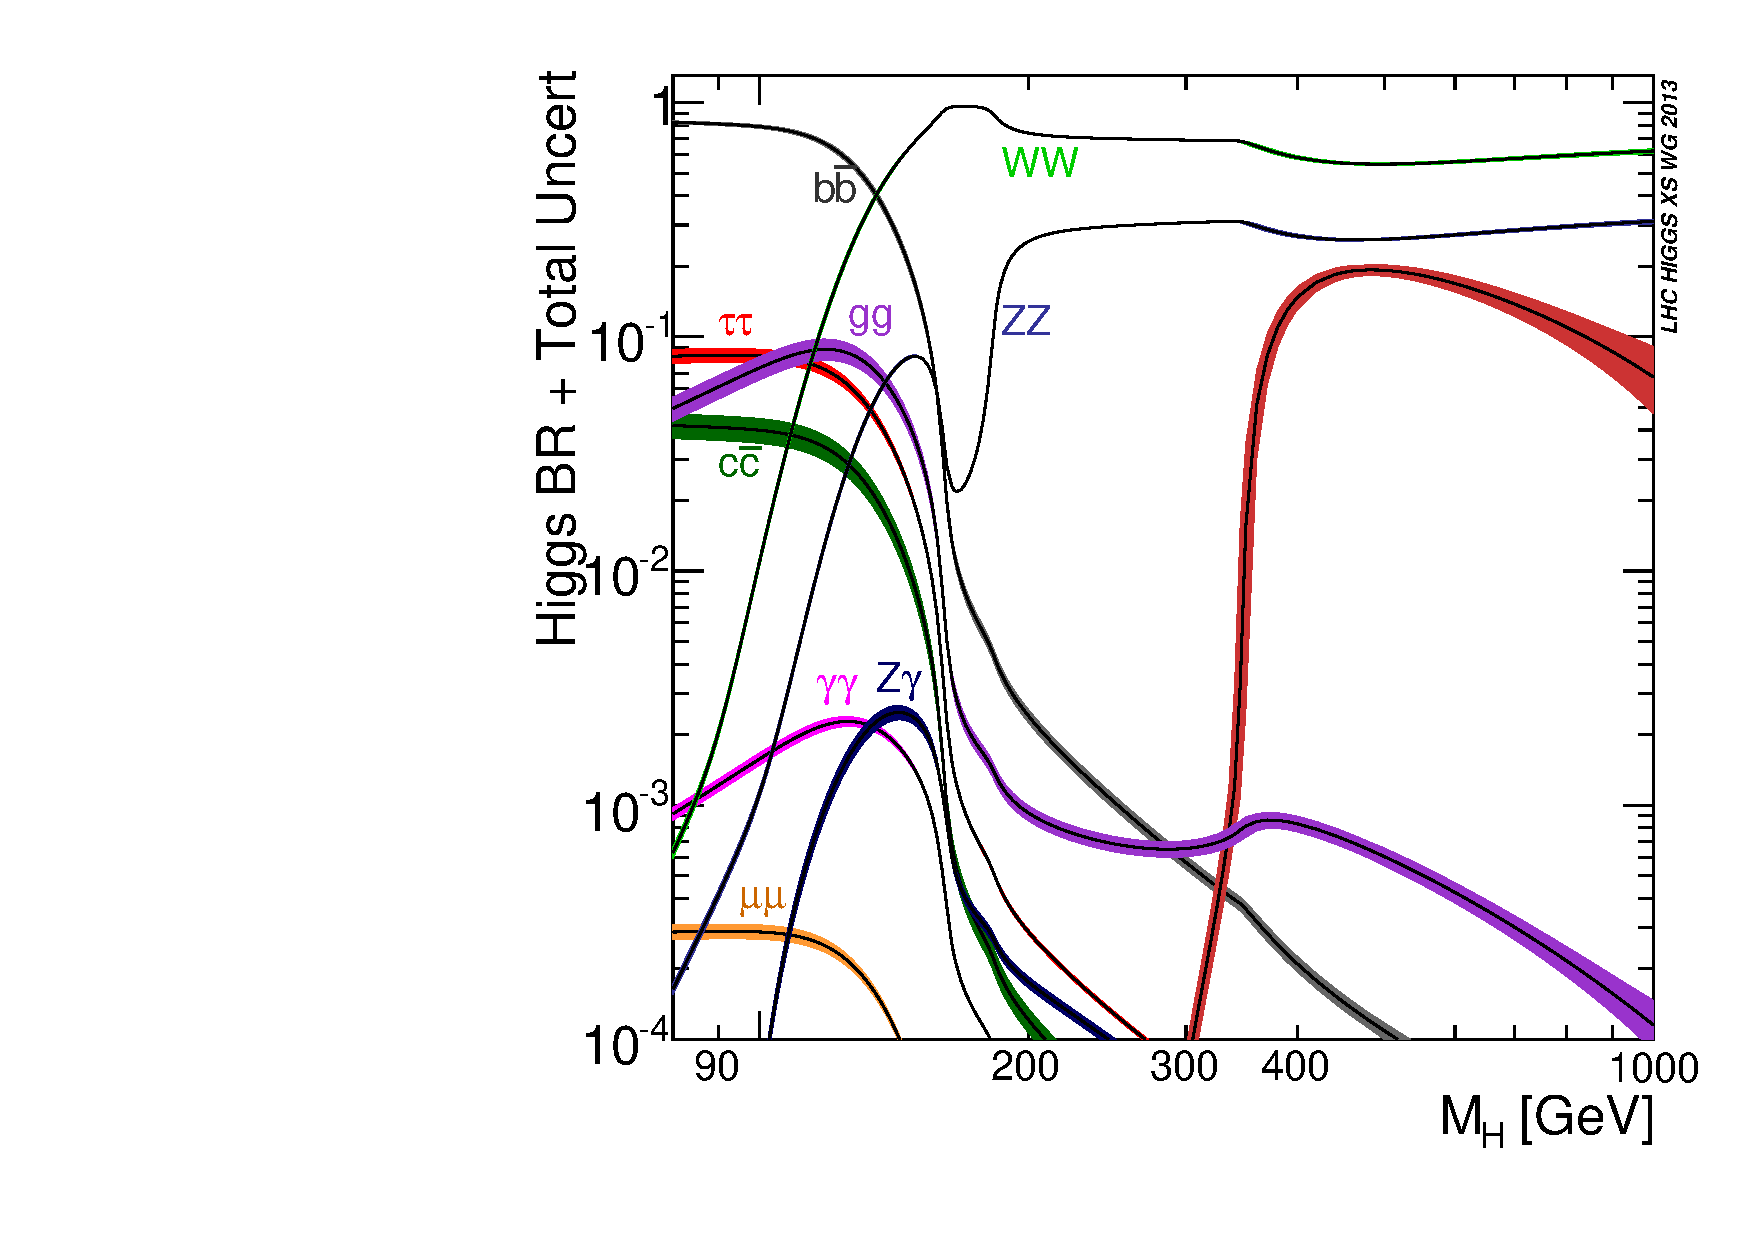
\includegraphics[width=0.8\textwidth,clip] {figures/Higgs_BR.pdf}
% \caption{Standard Model Higgs boson decay branching ratios as a function of mass.}
% \label{fig:HiggsBR}
% \end{figure}

% \begin{figure}
% \centering
% 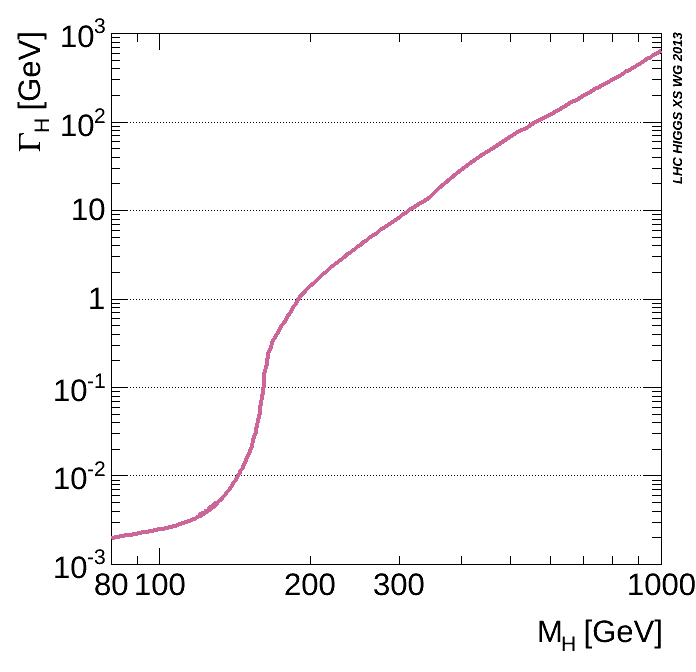
\includegraphics[width=0.8\textwidth,clip] {figures/SM_Width.png}
% \caption{Standard Model Higgs boson total width as a function of mass.}
% \label{fig:SMwidth}
% \end{figure}

\section{Properties of the Higgs boson}

% One method through which we can quantify possible deviations from our SM expectations is through precise measurements of properties of the Higgs. The Higgs boson is an extremely short-lived particle which rapidly decays into other lighter particles. Any such unstable particle has a finite lifetime $\tau$, which through the uncertainty principle is directly correlated to the width $\Gamma$ of its resonance, also interpreted as the uncertainty in its mass. Because the lifetime of a particle is set by its chance of decaying via various modes, the width of the Higgs boson can be influenced by deviations of the boson's couplings to other particles from our SM expectations. Thus precision measurements in the Higgs sector, especially of the Higgs' width, can act as indirect probes of new couplings. 

% For other particles with relatively broad resonances, the particles' width can be directly measured from a Breit–Wigner distribution over mass, which would peak around the particle's nominal mass. However, because the Higgs boson is so short-lived, its width is too narrow to be accurately measured from the line shape of this probability distribution. Even in the so-called ``golden channel'' of Higgs decay via H $\to$ ZZ$^*$ $\to$ $4\ell$ (named for its clean signature and good mass resolution), direct width measurement at the SM peak is limited by experimental resolution to about 1 GeV, far larger than the expected width of the Standard Model Higgs boson of around 4 MeV.

One of the most effective ways to investigate potential deviations from SM predictions is through precise measurements of the properties of the Higgs boson. As an extremely short-lived particle, the Higgs boson rapidly decays into lighter particles, and its finite lifetime \( \tau \) is inherently connected to the width \( \Gamma \) of its resonance via the uncertainty principle, \( \Gamma = \hbar / \tau \). This width can be interpreted as the intrinsic uncertainty in the particle's mass. Since the decay rate of the Higgs boson is dictated by its couplings to other particles, any deviation from SM predictions in these couplings would manifest as an alteration in its total width. Consequently, high-precision studies of the Higgs sector, particularly measurements of \( \Gamma_H \), provide an indirect but highly sensitive probe of BSM physics, including possible exotic decay channels or modifications to Higgs interactions.

For particles with broad resonances, the total width can be extracted directly from the Breit–Wigner line shape, which characterizes the probability distribution of invariant mass around the nominal mass of the particle. However, the Higgs boson presents a unique challenge in this regard. Due to its extremely short lifetime, the corresponding resonance width is remarkably narrow relative to its mass, making direct measurement from the line shape infeasible. Even in the so-called ``golden channel,'' where the Higgs decays via \( H \to ZZ \to 4\ell \) (a channel renowned for its clean experimental signature and excellent mass resolution), the finite detector resolution limits the direct width measurement to an uncertainty of approximately 1 GeV. This is orders of magnitude larger than the predicted SM Higgs boson width of around 4 MeV, rendering a direct determination of \( \Gamma_H \) at the peak practically impossible.

Given these limitations, alternative methods must be employed to infer the Higgs boson's width. One such approach involves off-shell Higgs boson production, where measurements in kinematic regions far from the Higgs boson pole mass can provide indirect sensitivity to its total width. This method separates Higgs boson-mediated and non-resonant background processes, and utilizes the observed yields of Higgs boson events to extract a measurement of \( \Gamma_H \) that is not constrained by detector resolution. The ability to probe the Higgs boson width through such indirect techniques represents a significant contribution to current precision Higgs boson studies in the ongoing search for deviations from the SM and potential new physics.

\section{Off-shell technique}

In this thesis, we employ the ``off-shell technique,'' originally developed by Caola and Melnikov~\cite{13074935} and implemented by the CMS collaboration~\cite{1405345570}, which currently provides the most stringent constraints on the Higgs boson total width. This method exploits Higgs boson production in two distinct kinematic regimes: the ``on-shell'' region, defined in this case within the invariant mass window of 105 to 140 GeV, and the ``off-shell'' region, characterized by Higgs boson candidates with masses exceeding 180 GeV.

A seminal study conducted in 2013 by researchers at Johns Hopkins University~\cite{13074935} demonstrated that the total width of the Higgs boson, \( \Gamma_H \), can be inferred by relating the production rates of on-shell and off-shell Higgs bosons. Specifically, by measuring the rate of Higgs production through gluon fusion and subsequent decay via the so-called ``golden channel'' (\( H^* \to ZZ \to 4\ell \)), a direct, resolution-constrained measurement of the Higgs width can be circumvented. Instead, a precise, statistically limited determination of \( \Gamma_H \) is achieved by taking the ratio of off-shell to on-shell Higgs event yields~\cite{190100174}. This relationship can be expressed as:

\begin{equation}
\label{eq:resonant}
\begin{gathered}
\sigma^\text{on-shell}_{VV \to H \to 4\ell} \propto \mu_{VVH} \frac{1}{\Gamma_H}, 
\quad\text{and}\quad
\sigma^\text{off-shell}_{VV \to H \to 4\ell} \propto \mu_{VVH},
\end{gathered}
\end{equation}

where \( \mu_{VVH} \) is the signal strength modifier, defined as the ratio of the observed to expected number of on-shell \( 4\ell \) events. Since the off-shell to on-shell Higgs boson cross-section ratio scales proportionally with \( \Gamma_H \), this method provides an indirect but highly sensitive probe of the Higgs boson width.

This approach offers several advantages. In the decay of an on-shell Higgs boson to a pair of massive vector bosons (e.g., \( ZZ \)), at least one of the \( Z \) bosons must be produced off-shell due to the Higgs boson mass being below the kinematic threshold of \( 2m_Z \approx 180 \) GeV. However, in the off-shell regime (\( m_H > 180 \) GeV), the Higgs boson can decay into two fully on-shell \( Z \) bosons, each with a mass of approximately 91 GeV. This results in a significant enhancement\footnote{This enhancement is only significant relative to the dramatic suppression of production as the Higgs boson moves off-shell. Overall, the off-shell range only accounts for $\sim14\%$ of the total number of Higgs boson events.} of the off-shell Higgs production rate at high invariant masses, thereby increasing the available event statistics and improving the precision of the width determination.

Furthermore, the focus on Higgs decays via the \( ZZ \to 4\ell \) channel ensures a clean experimental signature with excellent mass resolution, while also enhancing sensitivity to potential deviations in the Higgs' couplings to vector bosons. As a result, this method not only facilitates a precise measurement of the Higgs boson width but also serves as a robust probe of anomalous contributions to the Higgs–vector boson interaction vertex (\( HVV \)). With the LHC operating at a center-of-mass energy of 13.6 TeV in Run 3, the anticipated increase in high-energy collisions will further enhance the statistical power of this technique, enabling even more stringent tests of potential BSM physics.

% In this thesis, we will make use of the ``off-shell technique'' which was developed by CMS~\cite{1405345570} and is currently utilized in order to set the most precise limits on the Higgs boson width. This technique targets Higgs boson production in an ``on-shell'' region between 105 and 140 GeV and in an  ``off-shell'' region defined above 220 GeV. Higgs bosons are said to be produced ``on the mass shell'' if they exist close to the SM mass around 125 GeV and ``off-shell'' if they are produced away from their nominal mass, hence the names for the chosen mass ranges. 

% Through a method proposed by researchers at Hopkins in 2013~\cite{13074935}, it was shown that the width of the Higgs boson can relate the rate of on-shell Higgs boson production to the rate of off-shell production. By counting the number of Higgs bosons produced by strong or electroweak vector bosons ($v$) and that subsequently decay via the golden channel, we can forgo a direct measurement of the Higgs boson width and instead make a very precise width measurement by taking a ratio between the off-shell and on-shell Higgs yields~\cite{190100174}, the relation between which can be described with:
% \begin{equation}
% \label{eq:resonant}
% \begin{gathered}
% \sigma^\text{on-shell}_{vv \to H \to 4\ell} \propto \mu_{vvH}
% \quad\text{and}\quad
% \sigma^\text{off-shell}_{vv \to H \to 4\ell} \propto \mu_{vvH} \Gamma_H,
% \end{gathered}
% \end{equation}
% where $\mu_{vvH}$ is the ratio of the observed to expected number of on-shell $4\ell$ events.

% This approach comes with a few benefits. In the decay of an on-shell Higgs boson to two massive vector bosons (Z for example), one of the Z's must go off-shell since the SM Higgs boson mass is less than twice that of the Z boson. But for an off-shell Higgs with mass above 220 GeV, it is possible to decay via two on-shell Z bosons, each with mass around 90 GeV. Resultantly, we see an enhancement in the rate of Higgs boson production in our off-shell region at energies above what is required for vector boson pair production. This gives us significantly more statistics in our off-shell yield with which to make a precise width measurement. 

% Furthermore, because we are focusing on the Higgs decay via ZZ $\to$ $ 4\ell$, events in this off-shell region are very sensitive to variations in the Higgs' couplings to vector bosons. This means that while making a precise measurement of the Higgs boson width, we can indirectly probe at anomalous terms in the HVV amplitude. (And with the LHC targeting 13.6 TeV collisions in Run 3, we will have even more high-energy events at our disposal in the future.)

% ################################################################################################################

% \begin{figure}
% \centering
% 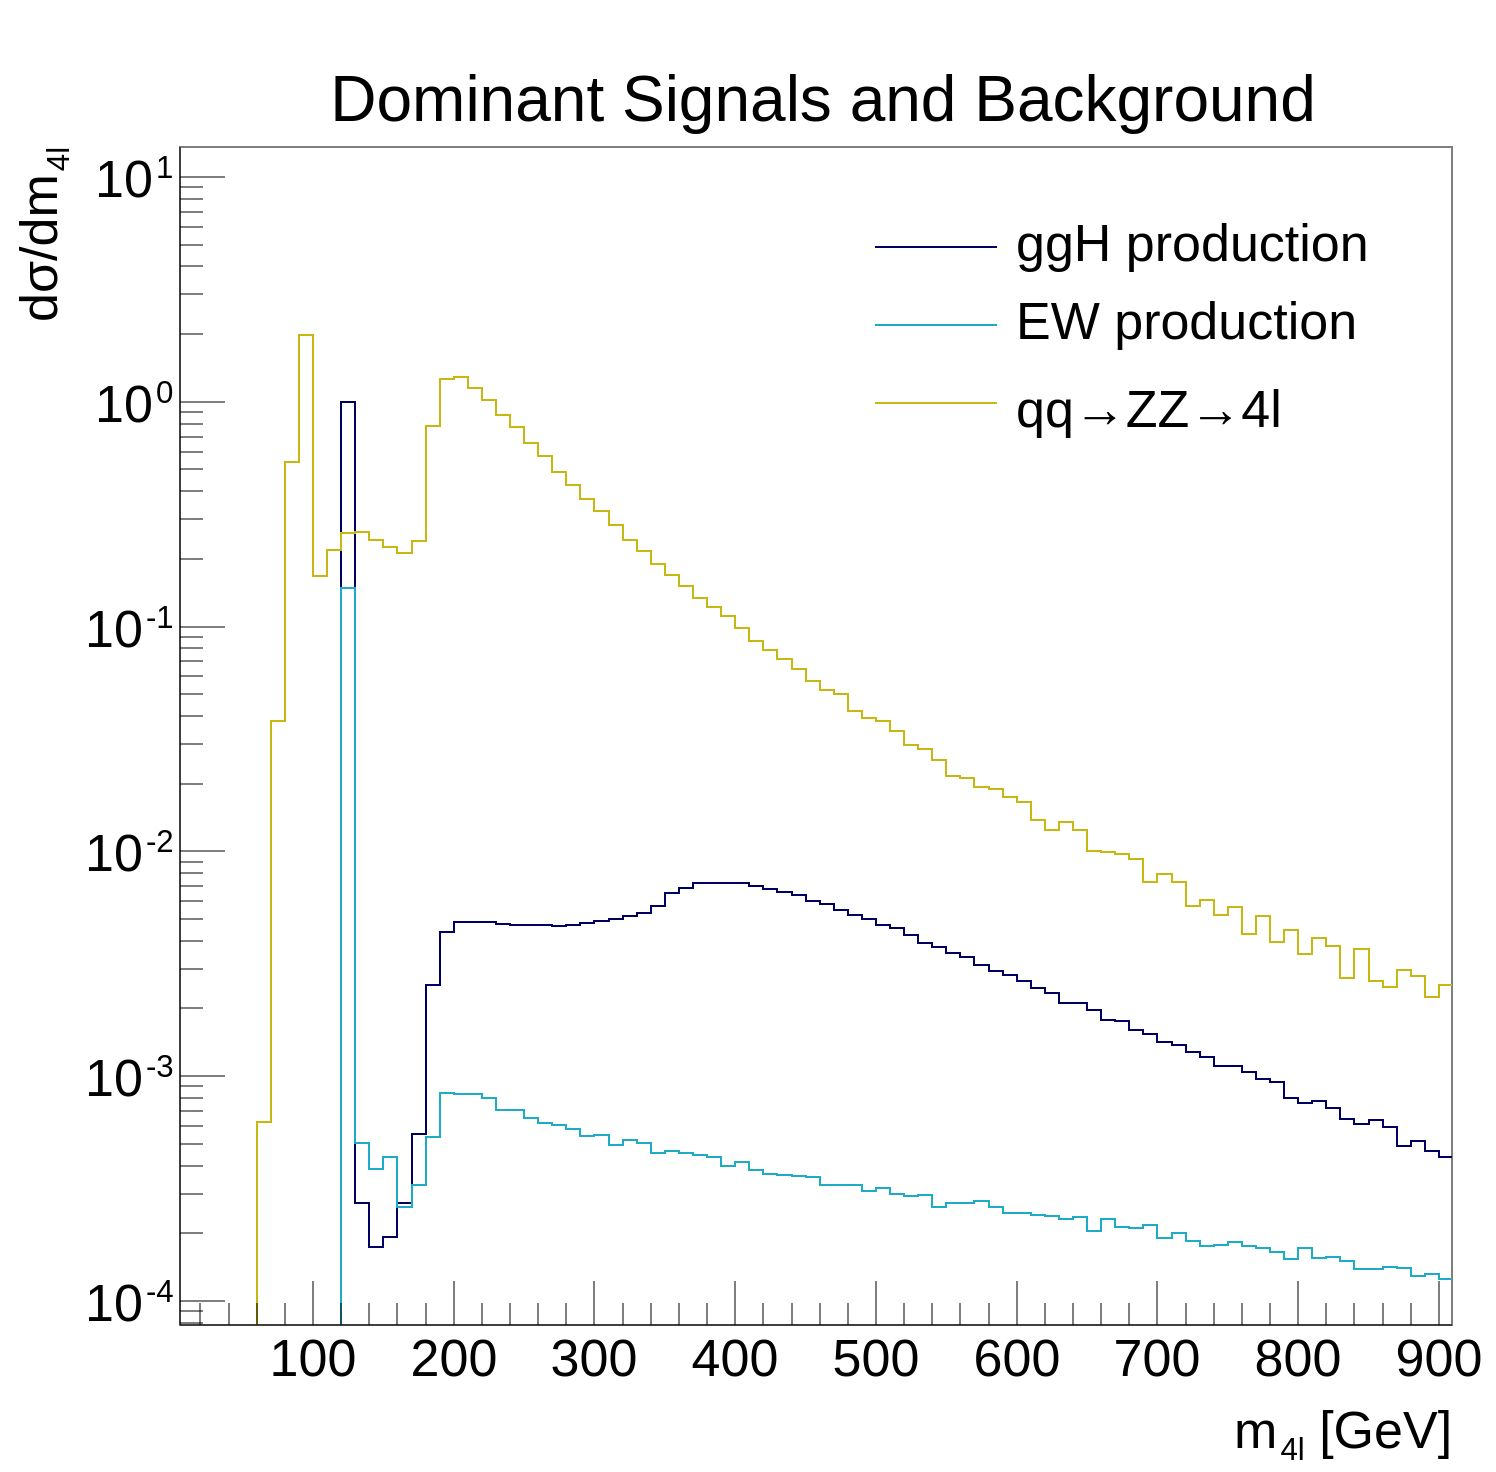
\includegraphics[width=0.8\textwidth,clip] {figures/offshell.jpg}
% \caption{}
% \label{fig:offshell}
% \end{figure}

% \subsection{Composite Higgs Boson}

\section{Higgs Boson Couplings}

In the SM, the Higgs boson couples to gluons via quark loops with Yukawa interactions, where the dominant contribution arises from the top-quark loop, as illustrated in Figure \ref{fig.ggH}. But BSM physics could allow for contributions from new heavy particles in this loop. %~\cite{Gonzalez-Alonso:2014eva,Greljo:2015sla}. 
Yukawa couplings also govern direct interactions with fermion-antifermion pairs, such as in $t\bar{t}H$ and $b\bar{b}H$ production. These interactions are less relevant at high energies due to their suppression, shown in Figure \ref{fig:prodModes}, but they are included in the analysis of on-shell Higgs production under similar assumptions as for gluon fusion.

The Higgs boson couples to the electroweak vector bosons in $HVV$ vertices, without the need for quark mediators. Since we are targeting off-shell Higgs boson production, we have one such vertex on the production sides of two of our primary Feynman diagrams, VBF and VH. And because of our focus on the \( H \to ZZ \) decay channel, we have additional $HVV$ vertices in all of our Feynman diagrams on the decay side. This makes us particularly sensitive to the $HVV$ amplitude overall, which we can use to our advantage.

Beyond the Higgs boson couplings to SM particles, we can also incorporate anomalous coupling strength terms which can be constrained to develop Effective Field Theory (EFT) descriptions. Some examples of familiar vertices in Feynman diagrams that can feature anomalous EFT contributions are shown in Figure \ref{fig:EFTdiagrams}. The anomalous contributions are treated as deviations in the Higgs boson's interactions with two gauge bosons. These anomalous couplings can manifest in both Higgs boson production and decay, regardless of the invariant mass at which the Higgs boson is produced. 
% Equation \ref{eq:resonant} is therefore meant to imply the simultaneous modifications of the $vvH$ couplings in both the on-shell and off-shell regions.
% The anomalous contributions are treated as deviations in the Higgs boson's interactions with two gauge bosons, including $WW, ZZ, Z\gamma, \gamma\gamma$, and $gg$.

\begin{figure}[!h]
\centering
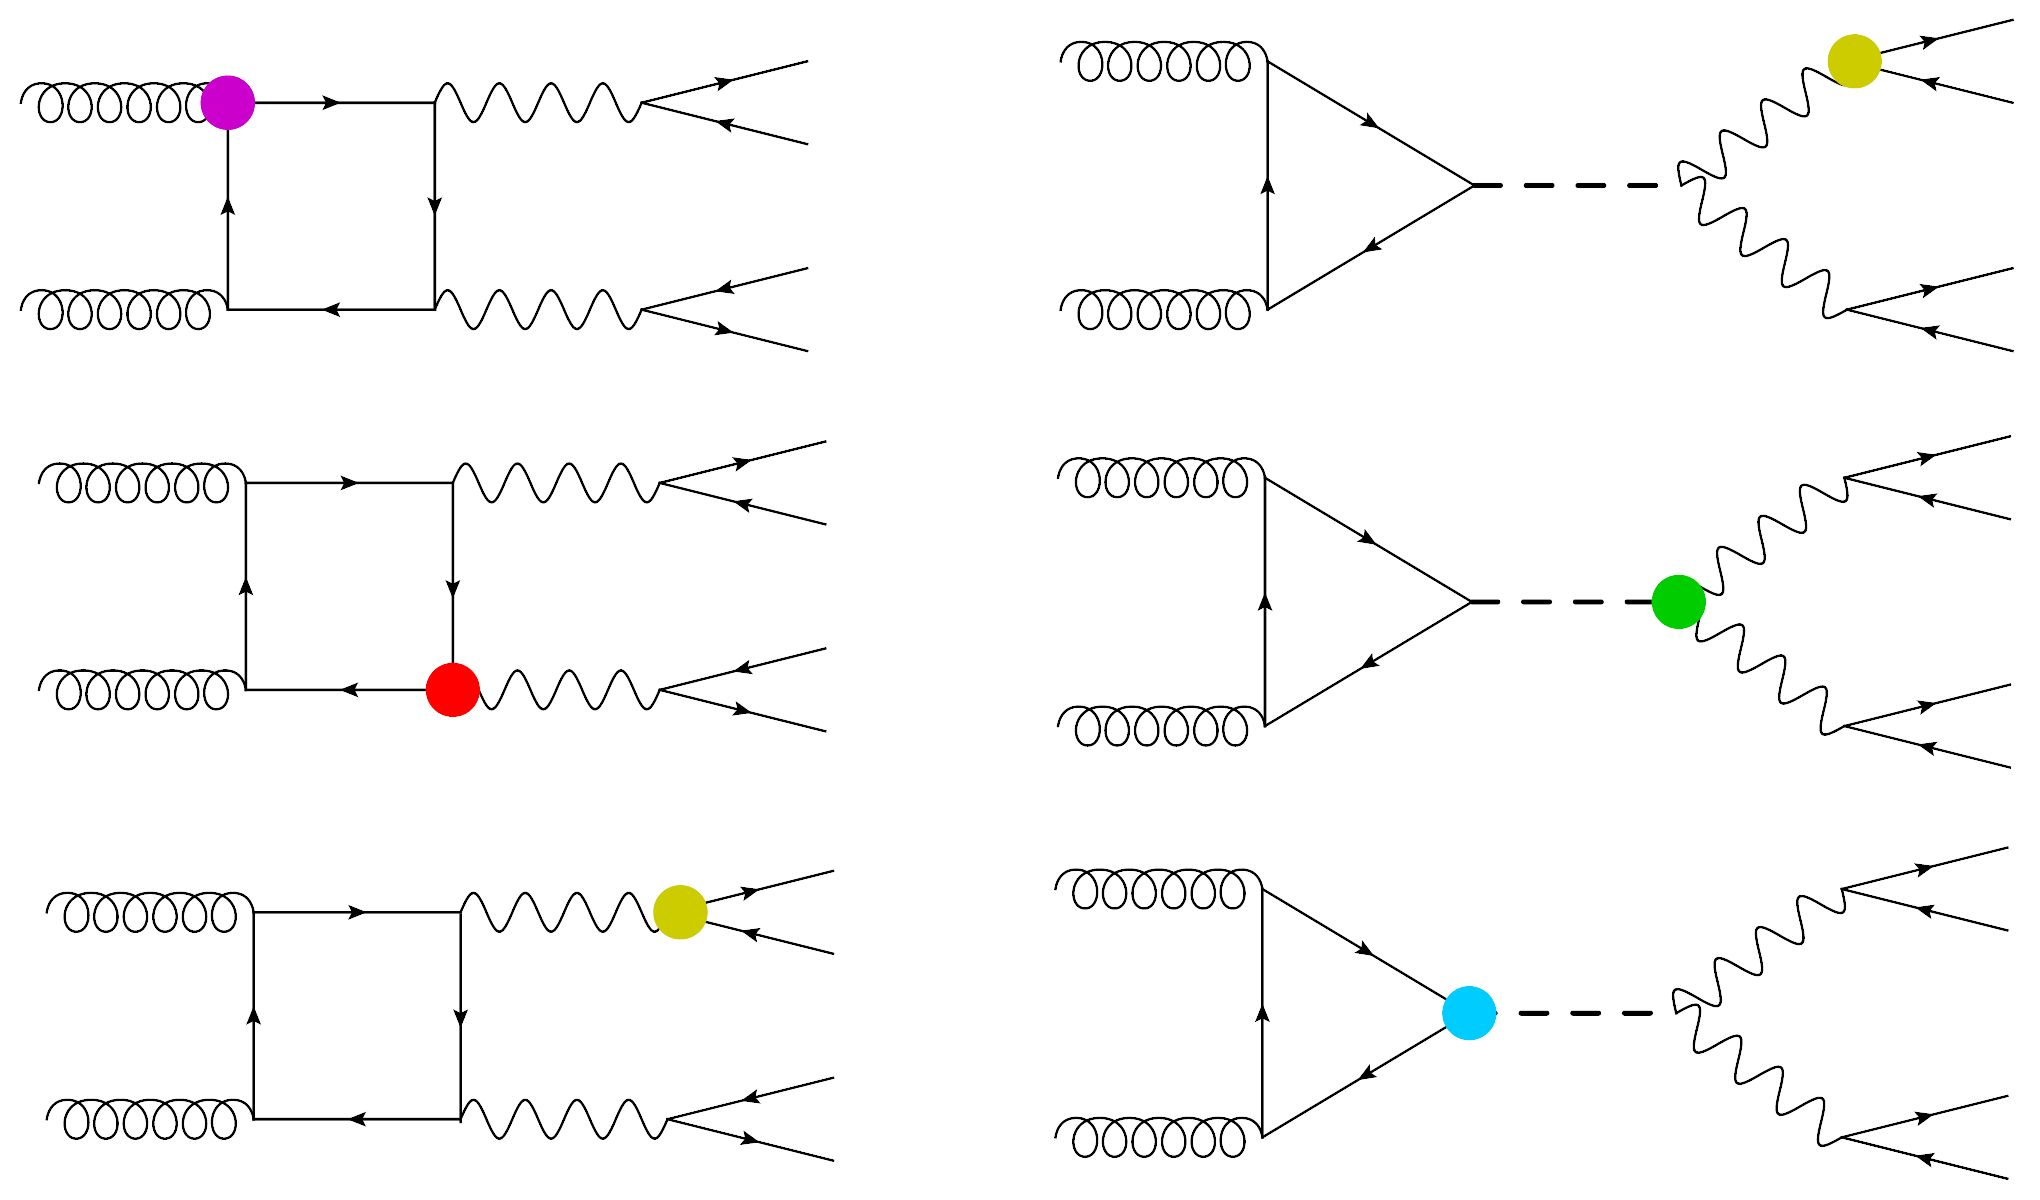
\includegraphics[width=0.8\textwidth,clip] {figures/EFTdiagrams.jpg}
\caption{Example Feynman diagrams for gluon fusion off-shell Higgs boson production and corresponding background with EFT insertions~\cite{offshellWGnote}.}
\label{fig:EFTdiagrams}
\end{figure}

% Anomalous contributions to the $HVV$ couplings may affect both the VBF and VH production mechanisms, as well as the Higgs boson decay into vector bosons. In the following discussion, we assume that the Higgs boson couples to two gauge bosons $VV$, such as $WW, ZZ, Z\gamma$, or $\gamma\gamma$, which in turn couple to fermions. These fermions appear either as four-lepton final states in Higgs boson decay, or as quarks and leptons in its production and in the decays of associated electroweak bosons.

% We assume that the Higgs boson does not couple to fermions via a new heavy state, which would generate a so-called contact interaction~\cite{Gonzalez-Alonso:2014eva,Greljo:2015sla}. However, the inclusion of amplitude terms corresponding to contact interactions is equivalent to testing anomalous $HVV$ couplings, as previously studied in~\cite{Khachatryan:2014kca}, under the assumption of flavor universality in $Vf\bar{f}$ interactions. Both approaches probe three general Lorentz-invariant tensor structures, with associated form factors $F_i(q_1^2,q_2^2)$, where $q_1$ and $q_2$ are the four-momenta of the two fermionic states, such as $(e^+e^-)$ and $(\mu^+\mu^-)$ in the $H \to e^+e^-\mu^+\mu^-$ decay, and analogous states in production.

% For this study, we fix all lepton and quark couplings to vector bosons to their SM values. While relaxing this assumption would allow for flavor non-universal couplings in the contact interaction terms, it would also introduce an excessive number of unconstrained parameters, making a meaningful test infeasible with the current data sample. We therefore restrict our analysis to the lowest-order operators, corresponding to the leading terms in the $(q_j^2/\Lambda^2)$ form-factor expansion, where $\Lambda$ denotes the energy scale of new physics.


% Even though we do not consider anomalous contributions in the \Hboson couplings to the SM particle
% in this version of analysis, let us still discuss those anomalous couplings for completeness, since they 
% will be constrained in the followup EFT analysis. 
% The treatment of anomalous couplings is based on a phenomenological framework 
% that describes the anomalous couplings of a Higgs-like boson
% to two gauge bosons, such as $\WW, \ZZ, \PZ\gamma, \gamma\gamma$ and $\glufu$.
% These couplings appear in either the production of the \Hboson or its decay,
% regardless of the \mell region in which the \Hboson is produced.
% The relationship in \Eq{eq:resonant} is therefore meant to imply concurrent variations
% in $\vv\PH$ couplings in both \onshell and \offshell regions.
% The coupling of the \Hboson to two gluons is assumed
% to be as in the SM, via quark loops with Yukawa couplings to quarks, where the contribution from the top-quark is dominant.
% This assumption is valid as long as the production is dominated
% by the top-quark loop and no new particles contribute to this loop.
% The Yukawa couplings also appear in direct interactions with fermion-antifermion pairs,
% such as in \ttH and \bbH productions. These interactions are of less importance in this study,
% since they are highly suppressed at high \offshell mass, but they are included in the analysis
% of the \onshell \Hboson production with similar assumptions as in the case of production via gluon fusion.
% Variation of the \HVV couplings, in either the \VBF or \VH~productions, or the \Hell decay,
% are allowed to depend on anomalous coupling contributions.

% In the following, we assume that the \Hboson couples to two gauge bosons \VV, such as
% \WW, \ZZ, $\PZ\gamma$ or $\gamma\gamma$, which in turn couple to fermions,
% either four leptons in \Hboson decay, or quarks or leptons in its production or in the decay
% of associated EW bosons. It is assumed that the \Hboson does not couple to fermions through
% a new heavy state, generating a so-called contact interaction~\cite{Gonzalez-Alonso:2014eva,Greljo:2015sla}.
% However, the inclusion of amplitude terms pertaining to contact interactions is equivalent to the
% anomalous \HVV couplings already tested~\cite{Khachatryan:2014kca} under the assumption
% of flavor universality in $\V\ffbar$ couplings.
% Both approaches test three general tensor structures allowed by Lorentz symmetry,
% with form factors $F_i(q_1^2,q_2^2)$ in front of each term,
% where $q_1$ and $q_2$ are the four-momenta of the two difermion states, such as $(\EE)$ and $(\MM)$ in the
% $\PH \to \EE\MM$ decay, and equivalent states in production. We also fix all lepton and quark couplings to vector bosons
% according to SM expectations. Relaxing this requirement would make it equivalent to flavor nonuniversal couplings of the contact terms,
% but would also introduce too many unconstrained parameters, which cannot be tested with the present data sample.
% Only the lowest order operators, or lowest order terms in the $(q_j^2/\Lambda^2)$ form-factor expansion, are tested,
% where $\Lambda$ is the energy scale of new physics.

\subsection{Amplitude EFT Couplings} \label{sec:amplitudeEFT}

We assume that the Higgs boson couples to two gauge bosons $VV$, such as $WW, ZZ, Z\gamma$, or $\gamma\gamma$, which in turn couple to fermions. These fermions appear either as four-lepton final states in the Higgs boson decay, or as quarks and leptons in its production and in the decays of associated electroweak bosons.

A general form of the signal scattering amplitude of the H boson with two vector bosons can be written in terms of polarization vectors $\epsilon_i$ and momenta $q_i$ of bosons $V_i$, with scalar tensor $f^{(i){\mu \nu}} = \epsilon_{i}^{\mu}q_{i}^{\nu} - \epsilon_{i}^\nu q_{i}^{\mu}$, as:

\begin{equation}
\label{eq:formfact-fullampl-spin0}
\begin{gathered}
A(HVV)\propto
\left[ a_{1}^{VV}
+ \frac{\kappa_1^{VV}q_{1}^2 + \kappa_2^{VV} q_{2}^{2}}{\left(\Lambda_{1}^{VV} \right)^{2}}
+ \frac{\kappa_3^{VV}(q_{1} + q_{2})^{2}}{\left(\Lambda_{Q}^{VV} \right)^{2}}
\right]
m_{V1}^2 \epsilon_{V1}^* \epsilon_{V2}^* \\
+ a_{2}^{VV}  f_{\mu \nu}^{*(1)}f^{*(2),\mu\nu}
+ a_{3}^{VV}   f^{*(1)}_{\mu \nu} {\tilde f}^{*(2),\mu\nu},
\end{gathered}
\end{equation}

such that the scales of BSM physics are set by $\Lambda_{1}$ and $\Lambda_{Q}$, and the $a_{2}^{VV}$ and $a_{3}^{VV}$ scaled terms provide CP-even and CP-odd contributions, which may be sensitive to evidence of CP violation. Figure \ref{fig:EFTdiagrams2} highlights the double $HVV$ vertex present in our electroweak Feynman diagrams.

When at least one of the gauge bosons $V$ is massive, $m_{V1}$ is the pole mass of that gauge boson. All the $a_i^{VV}$ (which denotes $a_{1}^{VV}$, $1/\Lambda_{1}$, $1/\Lambda_{Q}$, $a_{2}^{VV}$, and $a_{3}^{VV}$) terms act as coupling-strength modifiers on their corresponding contributions to the amplitude. In this general form, pure SM behavior is described by $a_{1}^{VV}$ alone.

% Under the assumption that the couplings are constant and real, Equation \ref{eq:formfact-fullampl-spin0} is equivalent
% to an effective Lagrangian notation. Therefore, in this paper, the real coupling constants are tested.
% The above approach allows a sufficiently general test of the \(H \to 4\ell\)
% kinematics in decay and equivalent kinematics in production, as discussed below, including production
% and decay of virtual intermediate photons. If deviations from the SM are detected,
% a more detailed study of $F_i(q_1^2,q_2^2)$ could be performed, eventually providing a measurement of the
% double-differential cross section for each tensor structure tested.

Instead of constraining $a_i$ directly, we can constrain the fractional contribution of the anomalous coupling to the signal scattering amplitude of the Higgs boson, as a ratio of observable cross sections $f_{ai}$. This has the benefit of being invariant to the $a_n$ coupling scale, and having values bounded by 0 and 1. Also, in experimental measurements of $f_{ai}$ most systematic uncertainties cancel in the ratios and we have a cleaner measurement~\cite{2020}. We define ratio $f_{ai}$ and phase $\phi_{ai}$ as:

\begin{equation}
\label{eq:faiandphase}
\begin{gathered}
f_{ai} = \frac{|a_i|^2 \sigma_i}{\sum_{j=1,2,3...}|a_i|^2 \sigma_j},   \phi_{ai} = arg(\frac{a_i}{a_1}).
\end{gathered}
\end{equation}

\begin{figure}[!h]
\centering
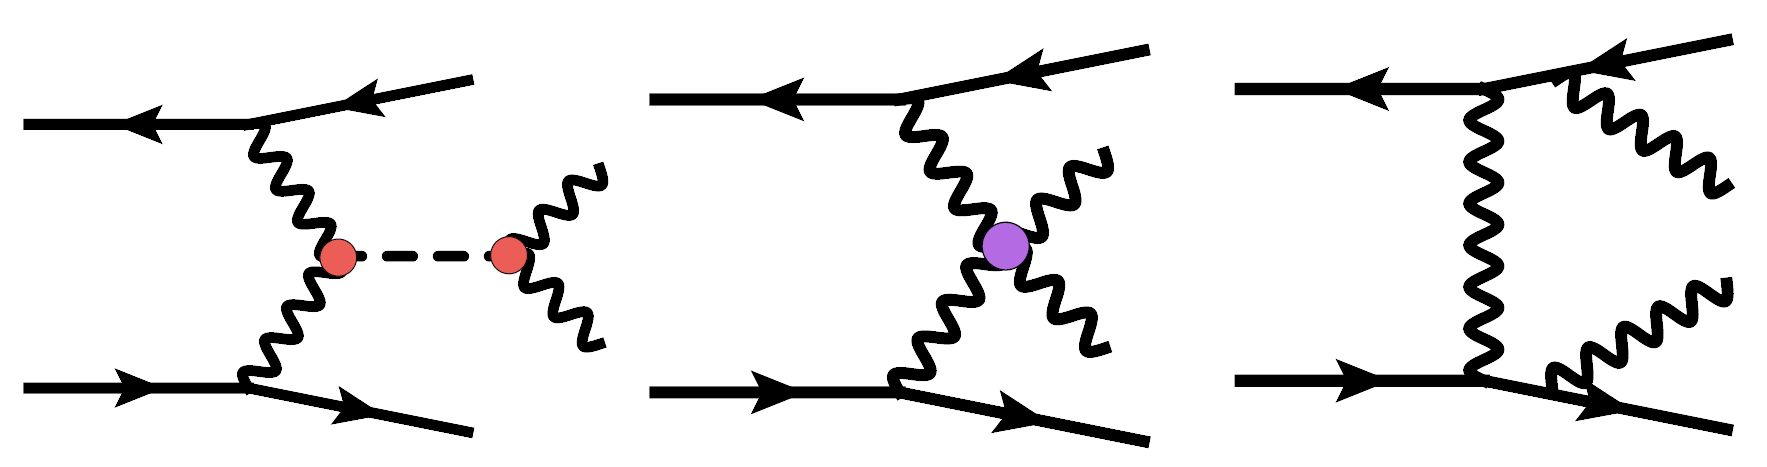
\includegraphics[width=0.8\textwidth,clip] {figures/EFTdiagrams2.jpg}
\caption{Example Feynman diagrams for electroweak off-shell Higgs boson production and corresponding background with EFT insertions~\cite{offshellWGnote}.}
\label{fig:EFTdiagrams2}
\end{figure}

\subsection{Kappa Framework Couplings} \label{sec:kappa}

Another representation of the Higgs boson couplings utilizes the so-called $\kappa$ framework, in which couplings of 
the Higgs boson to the SM particles are modified by a scale factor $\kappa_i$ for each particle $i$.

As previously discussed, SM-like behavior implies the top quark's predominance in the gluon fusion loop during Higgs boson production. If there are additional contributions in this loop, such as from undiscovered heavy particles, the probability distribution for Higgs boson production in the off-shell region would change. To model this, one could introduce a heavy quark~$\mathrm{Q}$ with coupling strength to the \Hboson $\kappa_\mathrm{Q}$~\cite{Gritsan:2020pib,Davis:2021tiv}.

In the framework of effective field theories, the contribution from $\mathrm{Q}$ can be reasonably interpreted as a point-like interaction which integrates all effects from heavy particles present in the loop.
One can include both top and bottom quarks in the loop, characterized by the coupling strength $\kappa_\mathrm{q}$, 
where $\kappa_\mathrm{q}=1$ corresponds to the SM. Similarly, $\kappa_\mathrm{V}$ is the \Hboson coupling strength to the $Z$ and $W$ bosons, which impact EW production and \Hboson decay and where $\kappa_\mathrm{V}=1$ in the SM. 

Using the $\kappa$ framework requires a re-parameterization of the signal strengths $\mu_F$ and $\mu_V$
in terms of $\kappa_\mathrm{q}$, $\kappa_\mathrm{Q}$, and $\kappa_\mathrm{V}$~\cite{Davis:2021tiv}:

\begin{equation}
\begin{aligned}
& \mu_V=\kappa_V^4\times\frac{\Gamma_0}{\Gamma} \\
& \mu_F=\kappa_q^2\kappa_V^2\times\frac{\Gamma_0}{\Gamma}
\end{aligned}
\label{eq:KappaMu}
\end{equation}

\begin{equation}
\begin{aligned}
& \kappa_Z = \kappa_W = \kappa_V= \mathrm{sign}(\mu_V)\left(|\mu_V|\Gamma/\Gamma_0\right)^\frac{1}{4} \\
& \kappa_t = \kappa_b = \kappa_q= \mathrm{sign}(\mu_F)|\mu_F|^\frac{1}{2} \left(\Gamma/(|\mu_V|\Gamma_0)\right)^\frac{1}{4}
\end{aligned}
\label{eq:KappaMu2}
\end{equation}

% On-shell pdf:
% \begin{equation}
% \begin{aligned}
% \mathcal{P}_{k}(\vec{x};\vec{\xi}_{k},\vec\zeta) =& \frac{(0.22 \kappa_Z^2 + 0.78\kappa_W^2 )\kappa_Z^2 \Gamma_0}{\Gamma_H}\mathcal{P}_{k}^\text{VBF sig} ( \vec{x};\vec{\xi}_{k}) \\
% &+\frac{( 0.3916\kappa_Z^2 + 0.6084\kappa_W^2 )\kappa_Z^2\Gamma_0}{\Gamma_H}\mathcal{P}_{k}^\text{VH sig} ( \vec{x};\vec{\xi}_{k}) \\
% &+\frac{\kappa_g^2\kappa_Z^2\Gamma_0}{\Gamma_H} \mathcal{P}_{k}^\text{ggf sig} ( \vec{x};\vec{\xi}_{k}) \\
% &+\frac{\kappa_t^2\kappa_Z^2\Gamma_0}{\Gamma_H} \mathcal{P}_{k}^\text{ttH sig} ( \vec{x};\vec{\xi}_{k}) \\
% &+ \mathcal{P}_{k}^\text{bkg}( \vec{x};\vec{\xi}_{k}),
% \end{aligned}
% \label{eq:Kappaponshell}
% \end{equation}

% Equation taken from~\cite{PhysRevD.105.096027}:
% \begin{equation}
% \begin{aligned}
% \kappa_g^2 =& 1.1068\kappa_t^2 + 0.0082\kappa_b^2 -0.1150\kappa_t\kappa_b \\
%             &+1.0298\kappa_Q^2 + 2.1357\kappa_t\kappa_Q - 0.1109\kappa_b\kappa_Q
% \end{aligned}
% \label{eq:kg2}
% \end{equation}

% Off-shell pdf:
% \begin{equation}
% \begin{aligned}
% \mathcal{P}_{k}(\vec{x};\vec{\xi}_{k},\vec\zeta) =&\kappa_Z^4~\mathcal{P}_{k}^{(VBF+VH)_{Z} \text{sig}} ( \vec{x};\vec{\xi}_{k}) \\
% &+\kappa_W^2\kappa_Z^2~\mathcal{P}_{k}^{(VBF+VH)_W \text{sig}} ( \vec{x};\vec{\xi}_{k})\\
% &+\kappa_W\kappa_Z^3~\mathcal{P}_{k}^{(VBF+VH)_{WZ} \text{sig}} ( \vec{x};\vec{\xi}_{k})  \\
% &+\kappa_Z^2~\mathcal{P}_{k}^{(VBF+VH)_Z \text{int}} ( \vec{x};\vec{\xi}_{k})  \\
% &+\kappa_W\kappa_Z~\mathcal{P}_{k}^{(VBF+VH)_W \text{int}} ( \vec{x};\vec{\xi}_{k})  \\
% &+\kappa_t^2\kappa_Z^2~\mathcal{P}_{k}^{ggF_{t} \text{sig}} ( \vec{x};\vec{\xi}_{k}) \\
% &+\kappa_Q^2\kappa_Z^2~\mathcal{P}_{k}^{ggF_{Q} \text{sig}} ( \vec{x};\vec{\xi}_{k}) \\
% &+\kappa_t\kappa_Q\kappa_Z^2~\mathcal{P}_{k}^{ggF_{tQ} \text{sig}} ( \vec{x};\vec{\xi}_{k}) \\
% &+(\kappa_t\kappa_Z)~\mathcal{P}_{k}^{ggF_{top} \text{int}} ( \vec{x};\vec{\xi}_{k}) \\
% &+(\kappa_Q\kappa_Z)~\mathcal{P}_{k}^{ggF_{Q} \text{int}} ( \vec{x};\vec{\xi}_{k}) \\
% &+\frac{\kappa_Z^4\Gamma_0}{\Gamma_H}~\mathcal{P}_{k}^\text{cross} ( \vec{x};\vec{\xi}_{k}) \\
% &+ \mathcal{P}_{k}^\text{bkg} ( \vec{x};\vec{\xi}_{k}),
% \end{aligned}
% \label{eq:Kappapoffshell}
% \end{equation}


The bulk of this thesis focuses on measurements of the SM Higgs boson, but it will also include an extension of the analysis which sets constraints on these $\kappa$ framework coupling strengths. We will also see how this analysis sets the stage for upcoming measurements of anomalous coupling strengths in our amplitude basis, presented in Section~\ref{sec:amplitudeEFT}.

\chapter{The Experiment} \label{chap:chap-3}


% epigraph after chapter heading
\epigraph{We are experimentalists.}{-- Andrei Gritsan}


%%%% MUST: add the citation for the chapter if it is a reprint



%% remove the following and add your chapter text here
\section{The Large Hadron Collider}


Since its first start-up on 10 September 2008, the Large Hadron Collider (LHC) has been the world’s largest and most energetic particle accelerator. It is so named because it is very large, consisting of a 27 km ring of superconducting magnets; accelerates hadrons, usually protons or ions; and collides these particles via two beams travelling in opposite directions, which intersect at four points along the circuference of the machine.

\begin{figure}[!ht]
    \begin{center}
        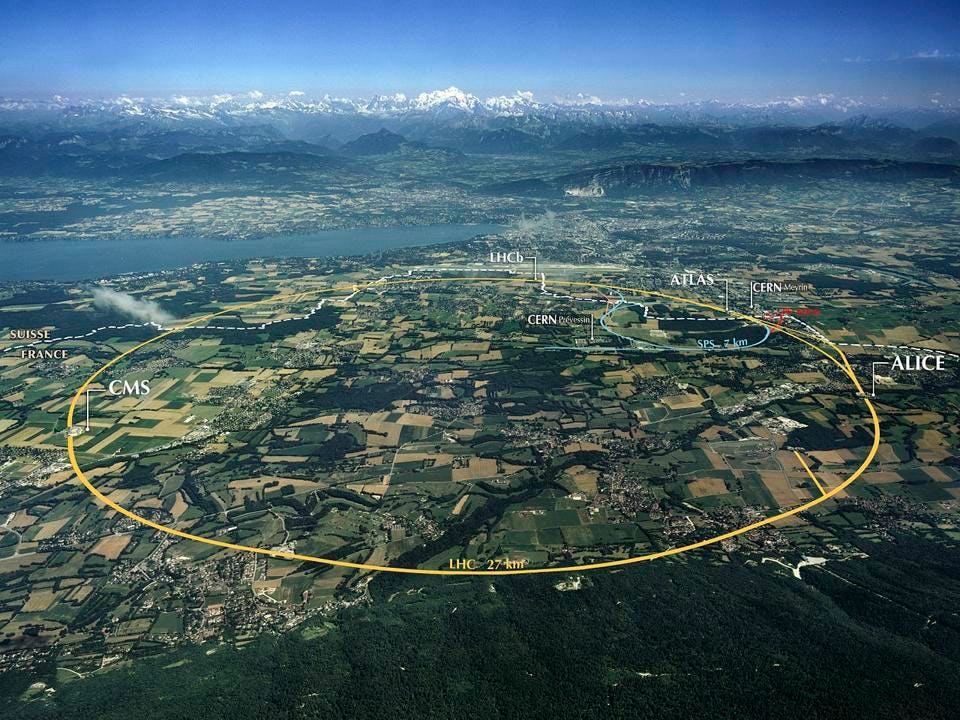
\includegraphics[width=0.8\textwidth,clip] {LHCaerial.jpg}
        \caption{An aerial view of CERN.}
        \label{fig:LHCaerial}
    \end{center}
    \end{figure}

The size of any accelerator is related to the maximum energy it can acheive. 
In the case of the LHC, this energy is proportional to the radius of the
machine and the strength of the magnetic fields that keep the accelerating particles stable. 
The LHC re-uses the 27 km circumference tunnel that was built for the previous big accelerator, the Large Electron-Positron Collider (LEP), which was dismantled in 2000.
The underground tunnel was the best solution to house a 27-km circumference machine because it was cheaper to excavate a tunnel rather than acquire the land to build at the surface.
In addition, the Earth’s crust provides good shielding for radiation. 
As such, the dimensions of the tunnel and capabilities of the magnets, cavities and other essential elements enforce the primary constraints which determine our design energy of 7 TeV per proton beam \cite{CERNBroc79}. 

The tunnel was built at a mean depth of 100 m, due to geological considerations (again translating into cost) and at a slight gradient of 1.4\%. 
Its depth varies between 175 m (under the Jura) and 50 m (towards Lake Geneva), as the LHC crosses the French-Swiss border.

\begin{table}[]
    \centering
    \begin{tabular}{|l|l|}
    \hline
    Design Parameter                & Value                                                                           \\ \hline
    Circumference                   & 26659 m                                                                        \\
    Dipole operating temperature    & 1.9 K (-271.3 ºC)                                                               \\
    Number of magnets               & 9593                                                                            \\
    Number of main dipoles          & 1232                                                                            \\
    Number of main quadrupoles      & 392                                                                             \\
    Number of RF cavities           & 8 per direction                                                                 \\
    Energy, protons                 & 7 TeV                                                                           \\
    Energy, ions                    & 2.76 TeV/u                                                                      \\
    Peak magnetic dipole field      & 8.3 T                                                                           \\
    Distance between bunches        & $\sim$7.5 m                                                                     \\
    Luminosity (protons)            & $10^{34} cm^{-2} s^{-1}$ \\
    No. of bunches per proton beam  & 2808                                                                            \\
    No. of protons per bunch        & 1.1 x 1011                                                                      \\
    Number of turns per second      & 11245                                                                           \\
    Number of collisions per second & 1 billion                                                                       \\ \hline
    \end{tabular}
    \caption{Design parameters for the LHC}
    \label{tab:LHCparam}
\end{table}

Superconducting electromagnets are specifically designed to generate a powerful magnetic field of 8.3 T around the circumference of the collider. LHC dipoles use niobium–titanium (NbTi) cables, which become superconducting below a temperature about 10 K (-263.2 °C)\footnote{The LHC actually operates at 1.9 K (-271.3 °C) and the beam pipes are kept at ultrahigh vacuum ($10^{-10}$ to $10^{-11}$ mbar), even colder than outer space (2.7 K or -270.5 °C) and close to the atmospheric pressure of the Moon's surface!}. Approximately 10000 superconducting magnets are installed in the LHC. Among these, 1232 dipole magnets, each 15 meters long, guide the beam around the accelerator ring, while 392 quadrupole magnets, each measuring between 5 and 7 meters, focus the beam. Additional stronger quadrupole magnets are positioned near interaction points\footnote{Just prior to collision, magnets will squeeze the particles closer together to increase the chances of collisions. The incoming particles are so small that the task of ensuring collision is akin to firing two needles 10 km apart with such precision that they meet halfway.}, along with multipole magnets to fine-tune the beam and refocus it after any deflection. The beam particles' energy is boosted by 0.5 MeV per turn using 16 radiofrequency (RF) cavities. To maintain the superconducting magnets at their operating temperature of 1.9K (-271.3°C), 96 tonnes of liquid helium is used. 

All the controls for the accelerator, its services, and technical infrastructure are housed under one roof at the CERN Control Centre. From here, the beams inside the LHC are steered to collide at four locations around the accelerator ring, corresponding to the positions of four particle detectors -- ATLAS, CMS, ALICE, and LHCb. Of these, CMS and ATLAS are general purpose detectors, while LHCb is sensitive to the physics of b quarks, and ALICE studies quark-gluon plasmas utilizing heavy-ion collisions.

The protons of the LHC circulate around the ring in well-defined bunches -- a direct consequence of the radio frequency (RF) acceleration scheme. 
Under nominal operating conditions, each proton beam has 2808 bunches, with each bunch containing about $10^{11}$ protons. 
The particles in these bunches are so small that the probability of any two colliding is very low. When the bunches cross at a colision point, there are up to 40 collisions between the total 200 billion particles. Bunches cross on average about 30 million times per second, so the LHC generates about 1 billion particle collisions per second.

This gives us our total design luminosity, which is the total number of proton-proton interactions. However, when studying a particular physics process, the probability of the process to occur in a given interaction is given by a factor which we call cross-section ($\sigma$). Thus the number of events per second created at the LHC for a certain physics process is calculated as:

\begin{equation}
\label{eq:crosssection}
\begin{gathered}
\frac{dN}{dt} = \mathcal{L} \times \sigma.
\end{gathered}
\end{equation}



\section{The Central Muon Solenoid}
The Central Muon Solenoid (CMS) detector is built around a large superconducting solenoid, for which it is named. It spans 6 meters in its internal diameter and generates a magnetic field of 3.8 Tesla. This very large field bends the trajectories of charged particles which helps to identify their momenta along with charge information. Inside the solenoid we find silicon trackers and calorimeters, while outside the solenoid we have layers of muon detection chambers.

\begin{figure}[!ht]
\begin{center}
    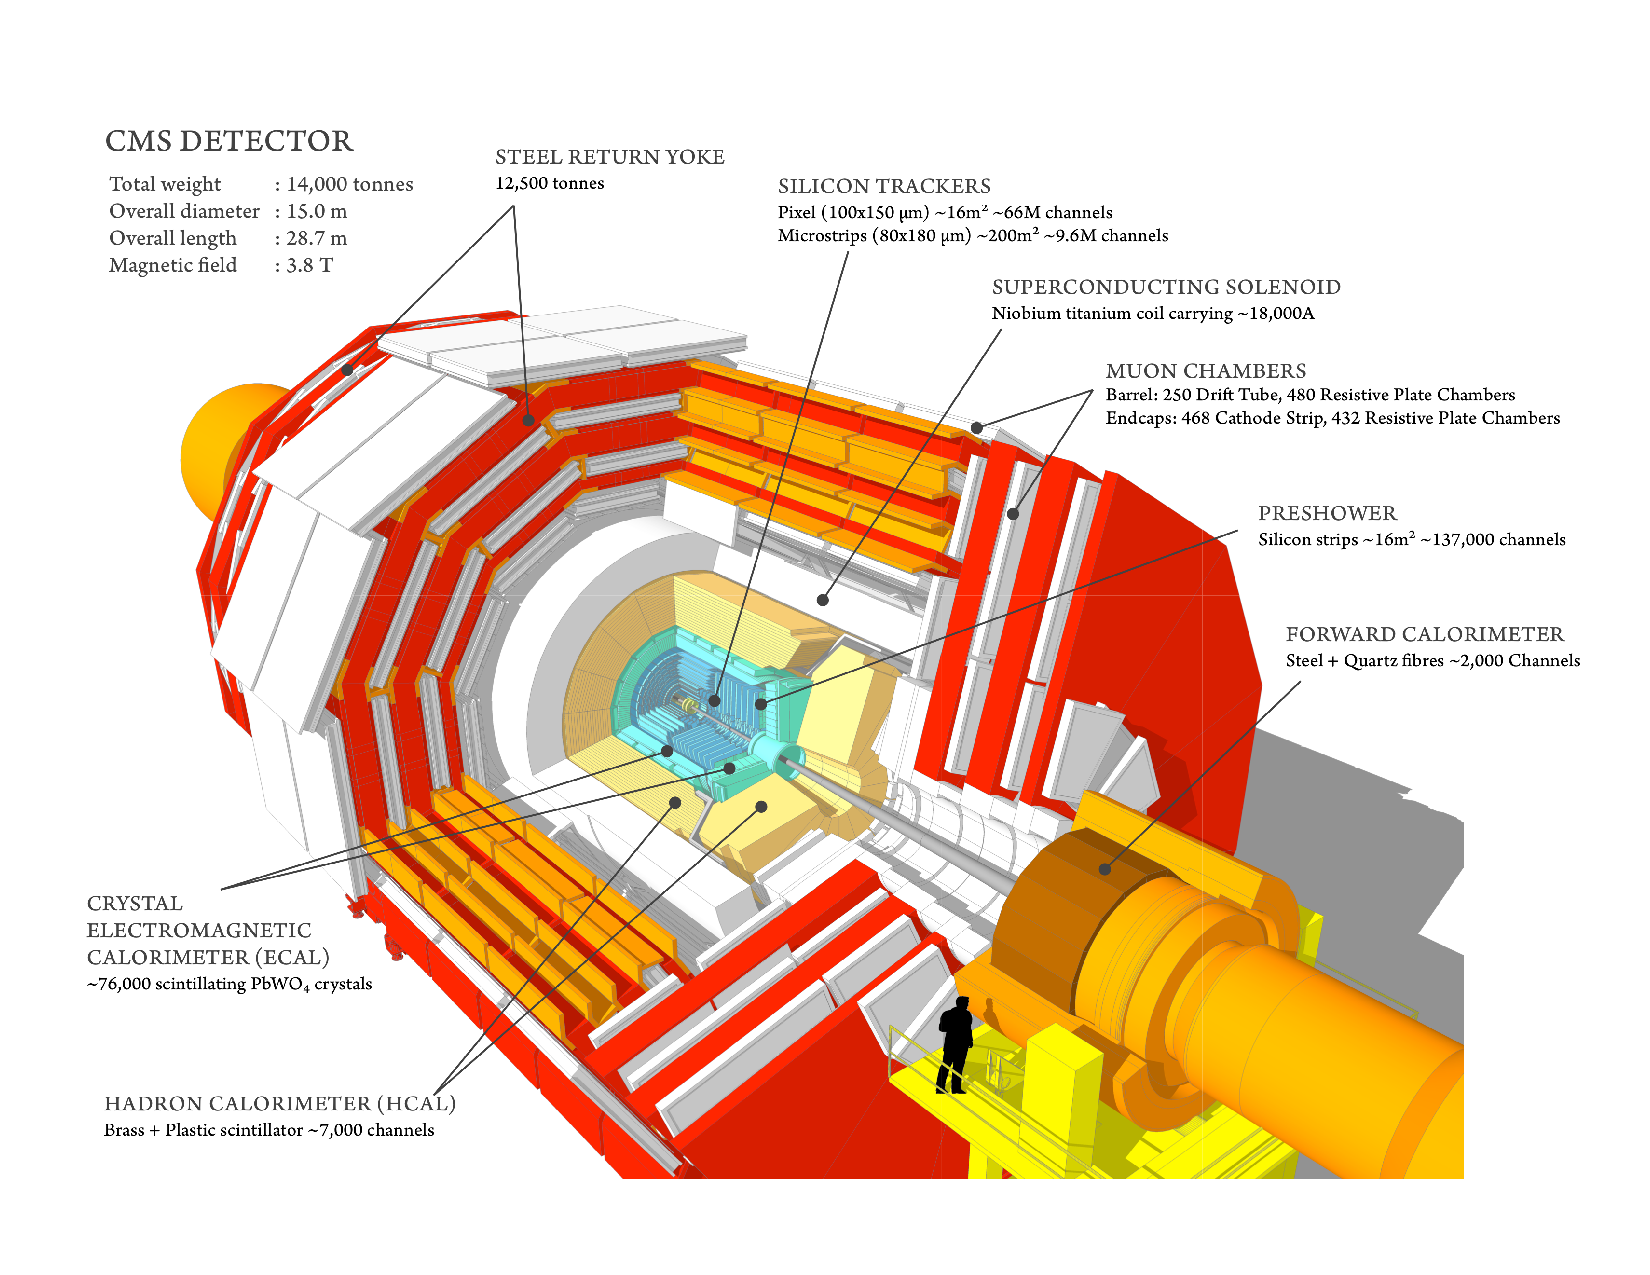
\includegraphics[width=0.8\textwidth,clip] {cmsdetector.pdf}
    \caption{The CMS detector is shaped like a cylindrical onion, with several concentric layers of components \cite{CMS}.}
    \label{fig:cmscutaway1}
\end{center}
\end{figure}

CMS in effect acts like a high-speed camera, taking 3-dimensional ``snapshots'' of particle collision events in all directions up to 40 million times each second. Although most of the initial collision products decay rapidly, the stable particles which they spawn can be detected by CMS. By identifying the stable particles produced in each collision and then piecing them together, the detector can recreate a picture of the collision which can then be analyzed to identify constituent physics phenomena \cite{Karimaki:368412, CERN-LHCC-2000-016, Chatrchyan:1129810, Collaboration:2745805, CERN-LHCC-2017-009}.

\subsection{Solenoid}
The superconducting solenoid is pivotal to the construction and operation of CMS, and has a 6 m internal diameter.
This magnet is the largest superconducting magnet ever built, weighing in at 12000 tonnes, and is cooled to -268.5ºC, almost as cold as outer space. 
The magnetic field of 3.8 T it generates is 100,000 times stronger than the Earth’s own magnetic field.

This large field is used to bend the paths of particles emerging from our high-energy collisions. Particles with more momentum have trajectories less affected by the magnetic field, so with high-precision position measurements from our tracking system and a precise tuning of such a strong magnetic field, we can make accurate measurements of the momentum of even high-energy particles. 

As previously mentioned, the tracker and calorimeter detectors (ECAL and HCAL) fit inside the magnet coil while the muon detectors are interleaved with a 12-sided iron structure that surrounds the magnet coils and contains and guides the field. Made up of three layers this structure, referred to as the ``return yoke,'' reaches out 14 m in diameter and also acts as a physical filter, through which only muons and weakly interacting particles such as neutrinos can traverse. The enormous solenoid also provides most of the experiment’s structural support, and is very robust to withstand the forces of its own magnetic field.

\begin{figure}[!ht]
    \begin{center}
        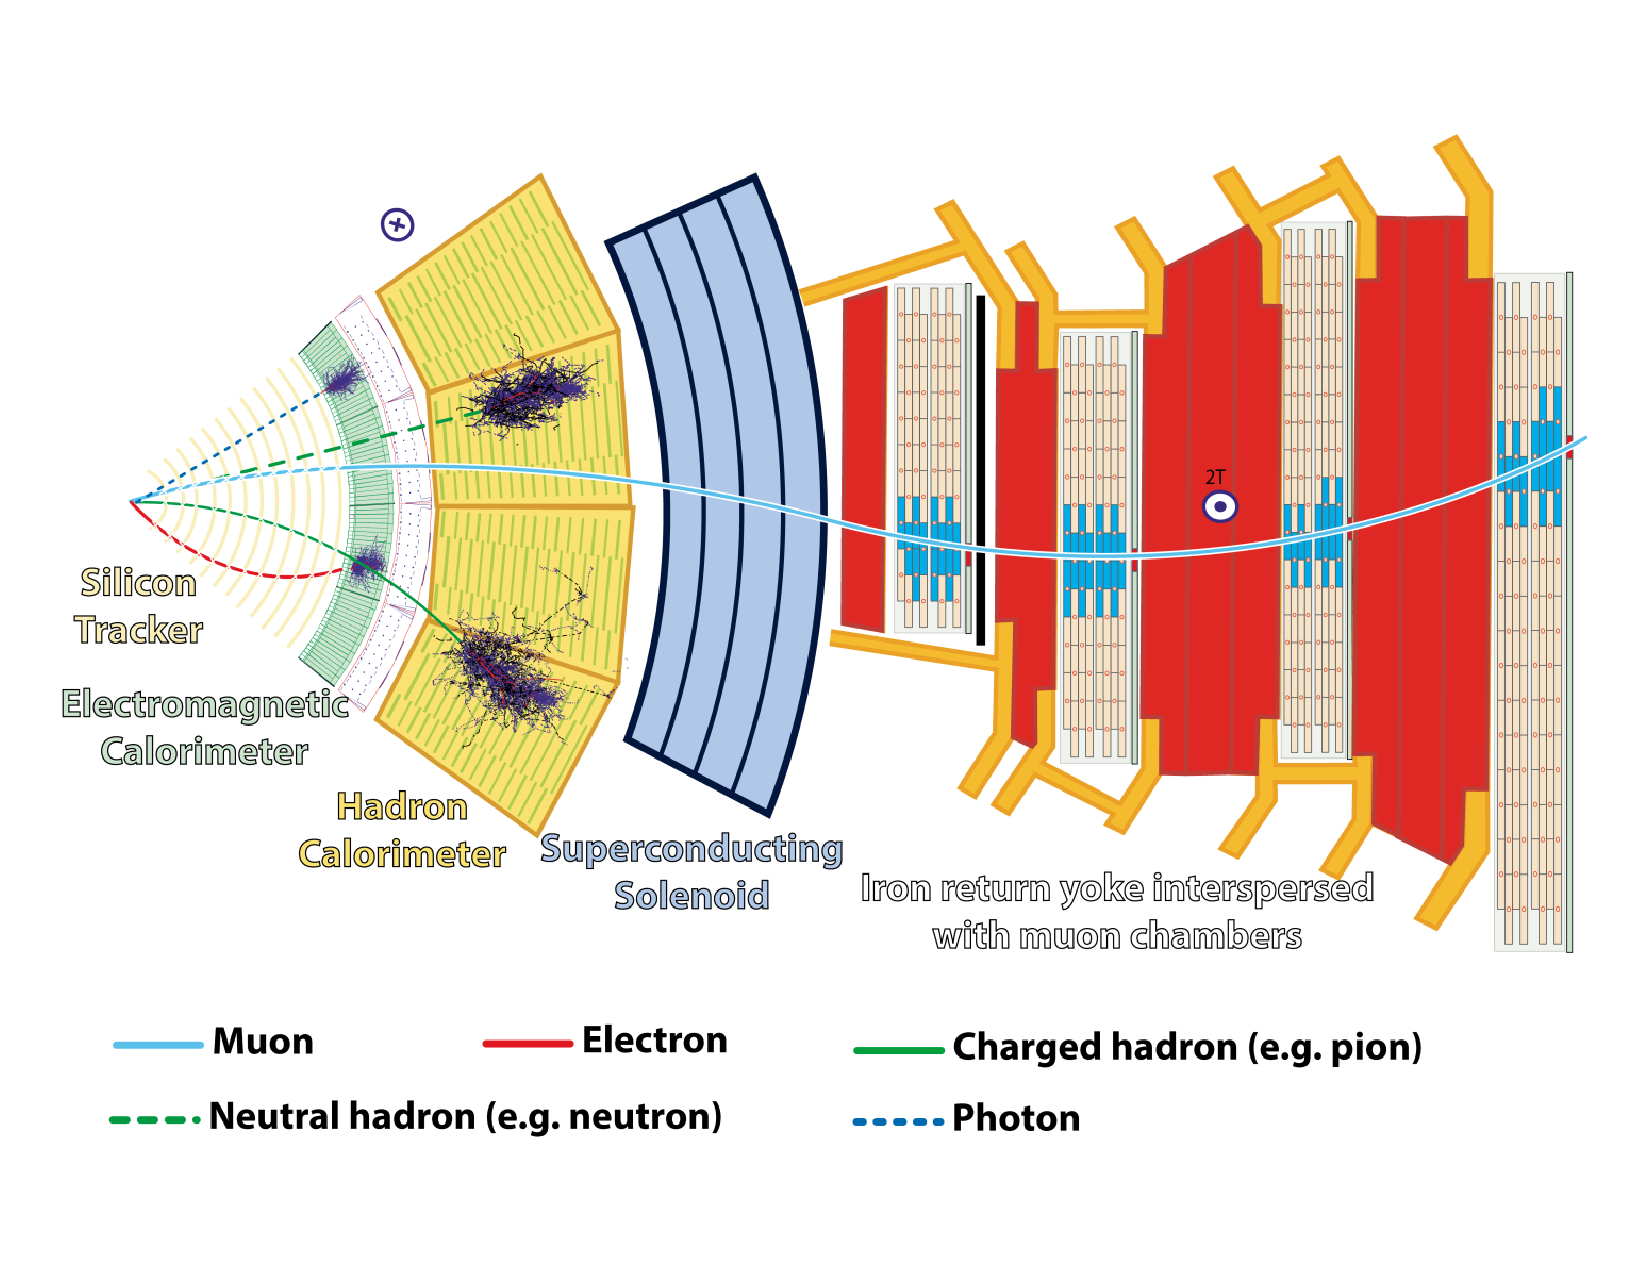
\includegraphics[width=0.8\textwidth,clip] {CMSslice.pdf}
        \caption{Schematic view of CMS detector \cite{CMS}.}
        \label{fig:cmscutaway2}
    \end{center}
\end{figure}

\begin{figure}[!ht]
    \begin{center}
        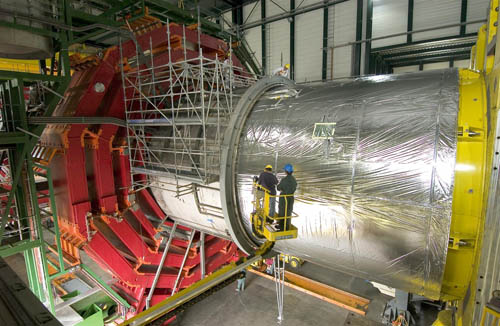
\includegraphics[width=0.8\textwidth,clip] {CMSmagnet.jpg}
        \caption{View of the CMS magnet during construction.}
        \label{fig:CMSmagnet}
    \end{center}
\end{figure}

\subsection{Silicon Tracker}

\begin{figure}[!ht]
    \begin{center}
        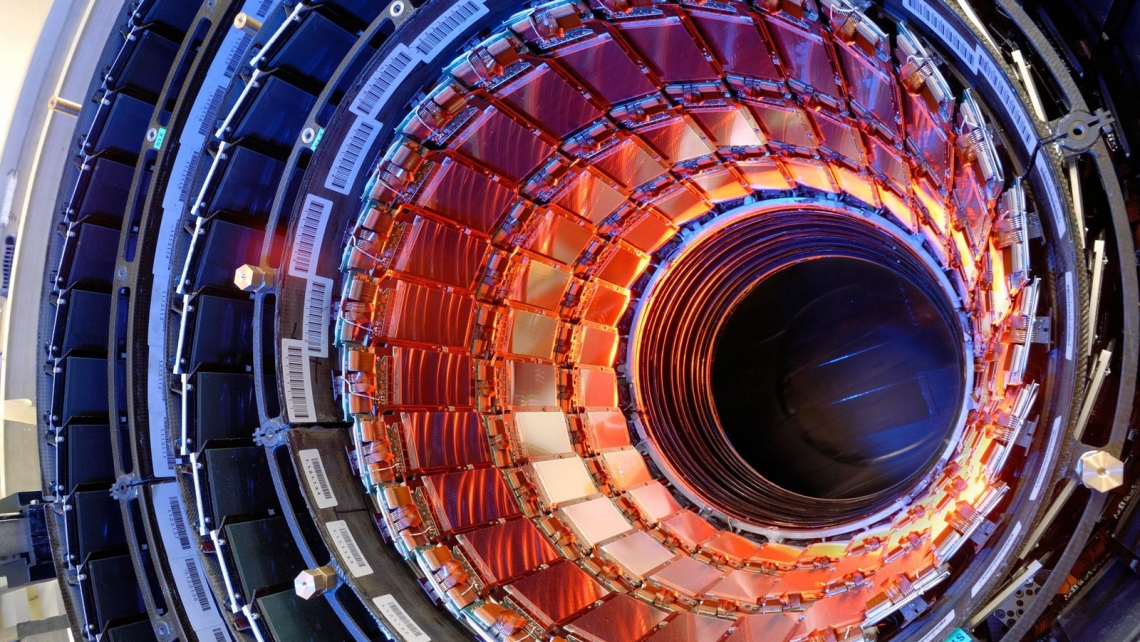
\includegraphics[width=0.8\textwidth,clip] {CMStracker.jpg}
        \caption{CMS Tracker showing silicon strips detectors in the barrel module.}
        \label{fig:CMStracker}
    \end{center}
\end{figure}

The tracker must precisely record particle paths while remaining lightweight to minimize interference with the particles. 
It achieves this by capturing highly accurate position measurements, allowing tracks to be reliably reconstructed with only a few data points. 
Each measurement has an accuracy of 10 µm, which is a fraction of the width of a human hair. 
As the innermost component of the CMS detector, the tracker is exposed to the highest volume of particles, so its construction materials were carefully selected for radiation resistance.

The tracker is assembled from several distinct detector elements, consisting of two silicon pixel subdetectors, the Tracker Pixel Barrel (TPB) and Tracker Pixel Endcap (TPE); 
and four silicon strip subdetectors, the Tracker Outer Barrel (TOB), Tracker Inner Barrel (TIB), Tracker Inner Disks (TID), and Tracker Endcap (TEC) \cite{Chatrchyan:1667597}.

\begin{figure}[!ht]
    \begin{center}
        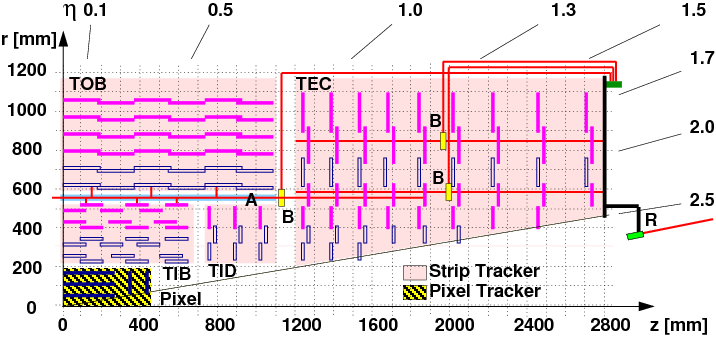
\includegraphics[width=0.8\textwidth,clip] {TrackerLayoutWithLAS.png}
        \caption{Schematic view of one quarter of the silicon tracker in the r-z plane.}
        \label{fig:CMStracker}
    \end{center}
\end{figure}


\subsubsection{Pixel Detector}

\begin{figure}[!ht]
    \begin{center}
        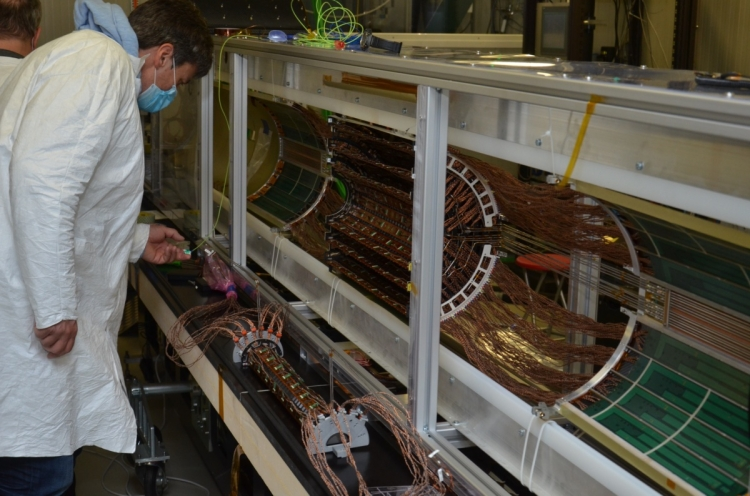
\includegraphics[width=0.8\textwidth,clip] {CMSpixel.jpg}
        \caption{Silicon pixel detector before installation.}
        \label{fig:CMSpixel}
    \end{center}
\end{figure}

\begin{figure}[!ht]
    \begin{center}
        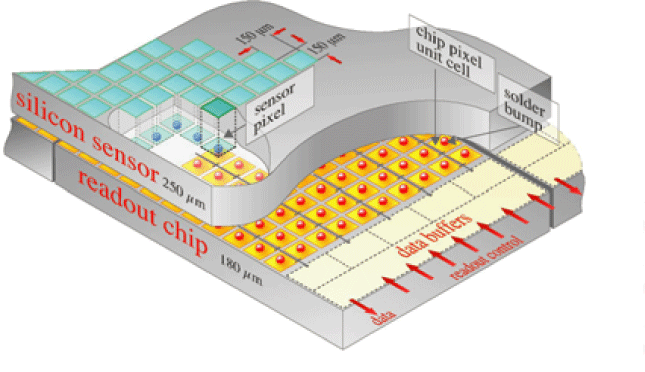
\includegraphics[width=0.8\textwidth,clip] {Pixelement.png}
        \caption{CMS silicon pixel detector.}
        \label{fig:CMSpixel}
    \end{center}
\end{figure}

The pixel detector, despite being only about the size of a shoebox, contains 124 million pixels, enabling it to track particle paths with exceptional accuracy as they emerge from collisions. 
Positioned closest to the beam pipe, it features cylindrical layers located approximately at radii of 3 cm, 7 cm, 11 cm, and 16 cm, with disks at either end. 
This proximity makes the pixel detector crucial for reconstructing the tracks of very short-lived particles.

Each of the four layers is composed of individual silicon modules, split into numerous pixels. Each of these silicon pixels is 100µm by 150µm, about the width of two human hairs. 
When a charged particle passes through a pixel, it ejects electrons from the silicon atoms. A voltage applied to the sensor allows the collection of these charges as a small electric signal, which is then amplified by an electronic readout chip (with a total of 16 chips per module). This design allows for significant bandwidth from the pixel detector, which is necessitated by the proximity to the point of collisions. The rate of particles received at 3 cm from the beamline is around 600 million particles per square centimeter per second.

Knowing which pixels have been energized allows us to deduce the particle's trajectory. And because the detector has 124 million of these pixels, arranged in four stacked layers of silicon modules, we can create a three-dimensional picture of each particle's path.


\subsubsection{Strip Detector}

\begin{figure}[!ht]
    \begin{center}
        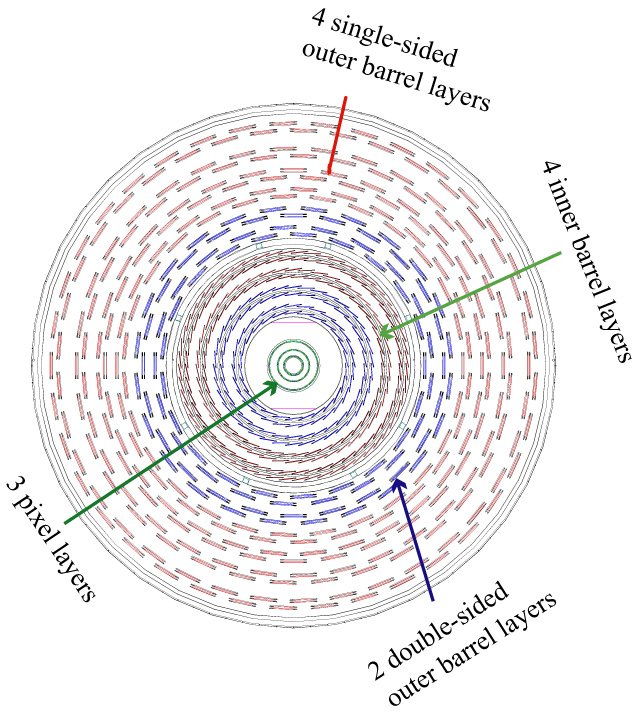
\includegraphics[width=0.8\textwidth,clip] {CMSBarrel.png}
        \caption{CMS Tracker layers shown in the plane perpendicular to the beam.}
        \label{fig:CMSBarrel}
    \end{center}
\end{figure}

After traversing the pixel detectors, particles move through ten layers of silicon strip detectors, which extend to a radius of 130 centimeters.

The silicon strip detector is composed of four inner barrel (TIB) layers and two inner endcaps (TID), each made up of three small discs. Surrounding both the TIB and TID is the outer barrel (TOB), consisting of six concentric layers. At either end of the tracker, two endcaps (TEC) provide closure. Each of these components contains silicon modules, wtih geometries optimized for their specific location within the detector.

This section of the tracker contains 15,200 highly sensitive modules, with a total of approximately 10 million detector strips read by 72,000 microelectronic chips. Each module comprises three main elements: one or two silicon sensors, a mechanical support structure, and readout electronics.

\subsection{Electromagnetic Calorimeter}

The Electromagnetic Calorimeter (ECAL) is the inner layer of the two calorimeters and measures the energy of electrons and photons by stopping them completely. 

\begin{figure}[!htb]
    \begin{center}
        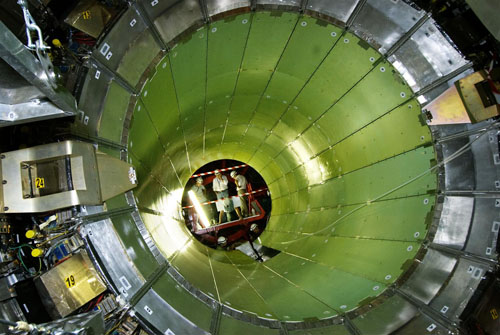
\includegraphics[width=0.8\textwidth,clip] {ECAL.jpg}
        \caption{CMS ECAL during construction.}
        \label{fig:ECAL}
    \end{center}
\end{figure}

The ECAL is constructed using nearly 80000 lead tungstate crystals, which are made primarily of metal (bound with oxygen in this crystalline form) and each weigh 1.5 kg. These crystals are incredibly dense yet highly transparent, and scintillate when electrons and photons pass through them. The light is produced in short, well-defined photon bursts which allows for precise identifications of the passing charged particles.

\subsection{Hadron Calorimeter}

Hadrons, which are composite particles made up of quarks and gluons, fly through the ECAL and are stopped by the outer layer called the Hadron Calorimeter (HCAL) \cite{CERN-LHCC-97-031}.

\begin{figure}[!htb]
    \begin{center}
        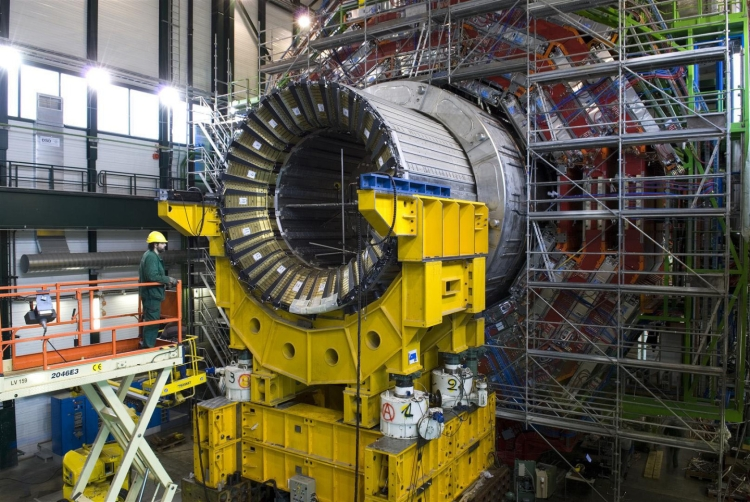
\includegraphics[width=0.8\textwidth,clip] {HCAL.jpg}
        \caption{Insertion of the HCAL barrel inside the magnet in 2008.}
        \label{fig:HCAL}
    \end{center}
\end{figure}

The HCAL is a sampling calorimeter meaning it finds a particle’s position, energy, and arrival time using alternating layers of dense ``absorber'' and fluorescent ``scintillator'' materials that produce a rapid light pulse when the particle passes through. Fitting the HCAL into the ``compact'' CMS required the use of very densely packed materials and geometry, since the minimum amount of material needed to contain and measure a hadron's shower is about one meter. 

To accomplish this feat, the HCAL is organised into barrel (HB and HO), endcap (HE), and forward (HF) sections. The endcaps are constructed from 36 ``wedges'' which measure particle energies as they emerge through the ends of the solenoid magnet. In addition, there are 36 barrel pieces, each weighing 26 tonnes, around the circumference of the barrel. These form the last layer of detectors inside CMS's magnet coil, since the outer barrel (HO) sits outside the coil to ensure that no energy escapes CMS undetected. 

Finally, the two hadronic forward calorimeters (HF) are positioned at either end of the detector, to capture any particles coming out of the collision region at large $\eta$, or shallow angles relative to the beam line. These receive the bulk of the energy from the particle collisions, so the HFs are very radiation hard.

\subsection{Muon System}

As its name suggests, detecting muons is one of the most important tasks of CMS. Muons are charged particles that are just like electrons and positrons, but 200 times heavier, and with much greater penetration depth. 
Because they can travel through several meters of material without losing much energy, unlike most created particles, they are not stopped by any of CMS calorimeters. Therefore, chambers specifically designed to detect muons are placed in the outer part of CMS, where they are likely to be the only particles producing a clear signal.



Muon hits are registered in the four muon stations, which are located outside of the magnet coil interleaved with the iron ``return yoke'' plates previously mentioned.

In total there are 1400 muon chambers: 250 drift tubes (DTs) and 540 cathode strip chambers (CSCs) track the particle positions and provide a trigger, while 610 resistive plate chambers (RPCs) and 72 gas electron multiplier chambers (GEMs) form a redundant trigger system, which quickly decides to keep or discard the acquired muon data. 


Muon tracking is achieved by measuring the curvature of muon trajectories in the $3.8\,\mathrm{T}$ magnetic field generated by the CMS solenoid.

The muon momentum is reconstructed by combining data from:
\begin{itemize}
	\item The muon chambers (for trajectory information).
	\item The silicon tracker (for high-precision tracking near the interaction point).
\end{itemize}
The combined resolution is approximately $3$--$5\%$ for transverse momentum $p_T > 10\,\mathrm{GeV/c}$.

The alignment of muon chambers is crucial for accurate tracking. Cosmic ray data and dedicated calibration runs are used to align the chambers to sub-millimeter precision.

Each detector type undergoes gas and electronic calibration to ensure timing and spatial measurements are accurate. This process includes:
\begin{itemize}
	\item Gas gain calibration for DT and CSC chambers.
	\item Timing calibration for RPC chambers.
\end{itemize}

\begin{itemize}
	\item The muon system achieves $>95\%$ detection efficiency for high-momentum muons.
	\item It integrates seamlessly with the calorimeters, inner tracker, and solenoid to provide a complete picture of collision events.
\end{itemize}

\subsubsection{Drift Tubes (DT)}
\begin{itemize}
	\item \textbf{Location:} DT chambers are located in the barrel region, covering a pseudorapidity range of $|\eta| < 1.2$.
	\item \textbf{Structure:} Each DT consists of parallel cylindrical drift tubes filled with a gas mixture, typically argon and carbon dioxide (CO$_2$).
	\item \textbf{Working Principle:} When a muon passes through a drift tube, it ionizes the gas. Electrons drift toward an anode wire under the influence of an electric field. The drift time provides precise position information.
	\item \textbf{Spatial Resolution:} Approximately $1$--$2\,\mathrm{mm}$.
	\item \textbf{Role:} DT chambers are used for both tracking and triggering, providing precise position and timing information.
\end{itemize}

\subsubsection{Cathode Strip Chambers (CSC)}
\begin{itemize}
	\item \textbf{Location:} CSCs are situated in the endcap regions, covering pseudorapidity ranges of $1.2 < |\eta| < 2.4$.
	\item \textbf{Structure:} Each CSC comprises multi-wire proportional chambers (MWPCs) with cathode strips for position readout.
	\item \textbf{Working Principle:} High-voltage differences between anode wires and cathode strips induce signals when muons pass through. Positions are reconstructed by measuring induced charge distributions.
	\item \textbf{Spatial Resolution:} Approximately $1\,\mathrm{mm}$ in the radial direction.
	\item \textbf{Role:} CSCs provide robust tracking in the forward region and contribute to the Level-1 (L1) trigger.
\end{itemize}

\subsubsection{Resistive Plate Chambers (RPC)}
\begin{itemize}
	\item \textbf{Location:} RPCs are deployed in both the barrel ($|\eta| < 1.6$) and endcap ($1.6 < |\eta| < 2.4$) regions.
	\item \textbf{Structure:} RPCs are made of resistive plates separated by a gas-filled gap. Typical gas mixtures include tetrafluoroethane (C$_2$H$_2$F$_4$) and sulfur hexafluoride (SF$_6$).
	\item \textbf{Working Principle:} Charged particles ionize the gas, creating avalanches that induce a fast signal across resistive plates.
	\item \textbf{Time Resolution:} Approximately $1\,\mathrm{ns}$.
	\item \textbf{Role:} RPCs provide fast timing information and are primarily used for triggering.
\end{itemize}


\begin{figure}
\centering
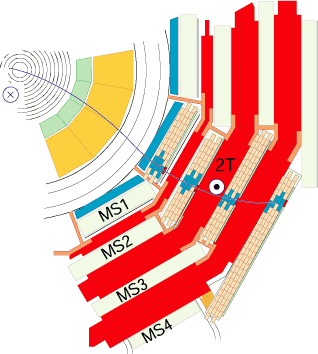
\includegraphics[width=0.80\textwidth]{figures/MuStations.png}
\caption{A muon, in the plane perpendicular to the LHC beams, leaves a curved trajectory in four layers of  muon ``stations.''}
\label{fig:MuStations}
\end{figure}    

\subsubsection{Muon Drift Tubes}

\begin{figure}
\centering
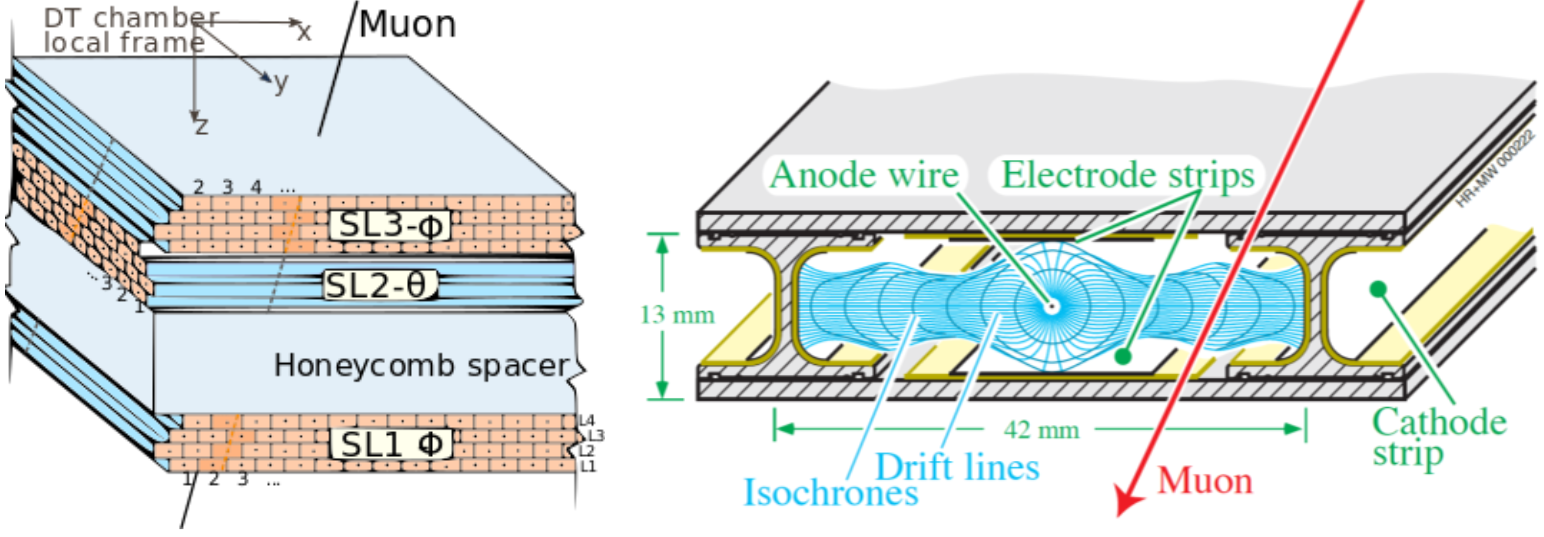
\includegraphics[width=0.80\textwidth]{figures/DTchambers.png}
\caption{The sizes of DT chambers range from  2m x 2.5m to 4m x 2.5m, approximately.}
\label{fig:DTchambers}
\end{figure}    

The drift tube (DT) system measures and identifies muon tracks in the barrel part of the detector. Each 4cm-wide tube contains a stretched wire within a gas volume. When a muon or any charged particle passes through the volume, it knocks electrons off the atoms of the gas. These electrons ``drift'' towards the anode following the electric field, ending up at the positively-charged wire where they are amplified and produce a measurable charge pulse. Each unit or ``superlayer'' contains four layers of staggered drift cells. By registering the time taken by the electrons to reach the wire, and since the drift velocity along the cell is a rather constant value, we can identify the exact crossing point of the muon along the cell.

\subsubsection{Cathode strip chambers}

\begin{figure}
\centering
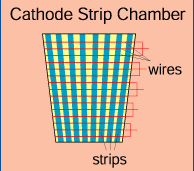
\includegraphics[width=0.80\textwidth]{figures/CSC.png}
\caption{}
\label{fig:CSC}
\end{figure}    

Cathode strip chambers (CSCs) are utilized in the endcap disks where the magnetic field is uneven, and particle rates are higher compared to the barrel. The chambers are made up of arrays of positively-charged anode wires intersecting with negatively-charged copper cathode strips within a gas-filled chamber. 

When muons pass through the chamber, they ionize the gas atoms, causing electrons to be knocked free. These electrons are attracted to the anode wires, creating an avalanche effect. Meanwhile, the positive ions move away from the wires and toward the copper cathode strips, generating a charge pulse in the strips, which occurs at a right angle to the direction of the wires. Since the wires run perpendicular to the strips, we get two position coordinates for each passing particle.

\subsubsection{Resistive Plate Chambers}

\begin{figure}
\centering
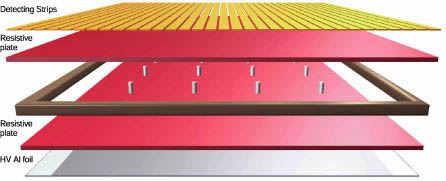
\includegraphics[width=0.80\textwidth]{figures/RPClayers.jpg}
\caption{}
\label{fig:RPClayers}
\end{figure}

Resistive Plate Chambers (RPCs) are fast gaseous detectors that provide a muon trigger system, consisting of two parallel plates acting as an anode and cathode. The plates are both made of a very high resistivity plastic material and separated by a thin gas volume.

\subsubsection{Gas Electron Multipliers}

\begin{figure}
\centering
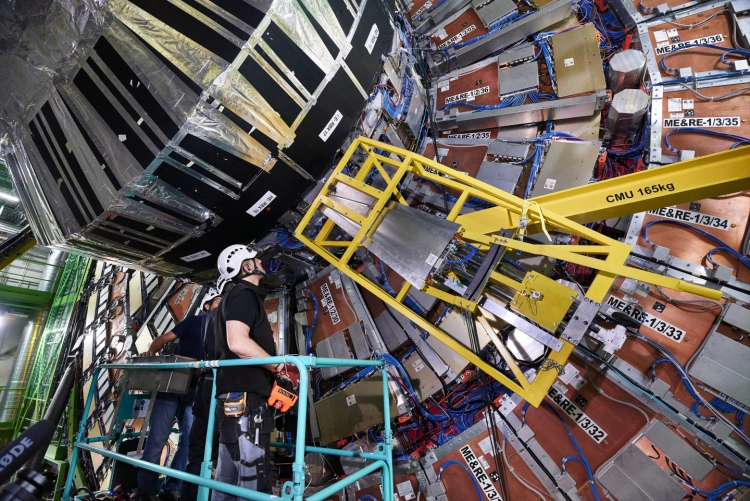
\includegraphics[width=0.80\textwidth]{figures/GEMinstallation.jpg}
\caption{Gas Electron Multiplier chamber installation.}
\label{fig:GEMinstallation}
\end{figure}

Gas electron multipliers (GEMs) are a new addition to the CMS muon system. They complement existing detectors in the forward regions close to the beampipe, where large radiation doses and high event rates will increase during Phase-2 of the LHC.

Like the other CMS muon subsystems, GEMs are gaseous detectors. Their key feature is the GEM foil, which consists of a 50 micrometer-thick insulating polymer (polyimide) surrounded on the top and bottom with copper conductors. Throughout the foil, microscopic holes are etched in a regular hexagonal pattern. The CMS GEM chambers consist of two PCBs, containing the gas volume, and a stack of three GEM foils in between. The chambers are filled with an Ar/CO2 gas mixture, which is ionized by incident ionizing particles. A potential difference applied across the foils generates sharp electric fields in the holes. The electrons created during the ionisation process drift towards the foils and are multiplied in the holes. The resulting electron avalanche induces a readout signal on the finely spaced strips.

\section{Triggers and Data Acquisition System}

Level 1 of the trigger is an extremely fast and wholly automatic process that looks for simple signs of interesting physics, e.g. particles with a large amount of energy or in unusual combinations.

One consequence of the decision was that L1 has to be more efficient than in previous systems in order to perform certain tasks traditionally performed by L2.

The muon chambers contribute significantly to the CMS trigger system, which is essential for selecting interesting collision events in real-time.

\subsection{Level-1 Trigger}
The L1 trigger uses coarse information from the DT, CSC, and RPC subsystems to identify high-transverse-momentum ($p_T$) muons. It operates within a latency of a few microseconds.

\subsection{High-Level Trigger (HLT)}
The HLT refines L1 trigger candidates by combining muon chamber data with inner tracker information. This process involves more sophisticated algorithms for precise momentum reconstruction.




\section{Computing}

Even with the triggers reducing the amount of unnecessary data coming out of our detector, CMS still produces a huge amount of data that must be analysed -- more than 5 Pb per year when running at peak performance.

The ``Tier 0'' center at CERN is the first to reconstruct full collision events, where analysts begin searching for patterns in the data. 
Then, after CERN creates a primary backup, the data is sent to large ``Tier 1'' computer centers located in seven different countries: France, Germany, Italy, Spain, Taiwan, the UK, and the US. 
At these centers, the events are reconstructed again, with improved calculations using refined calibration constants based on experimental information.

Tier 1 centers begin to interpret and analyze the particle events, compiling the results to identify emerging patterns. Simultaneously, each Tier 1 center sends the most complex events to a network of around 40 ``Tier 2'' facilities for further specialized analysis. This tiered system efficienty processes all CMS data while also allowing information to be distributed globally, regularly updated by the LHC Computing Grid.

\section{Particle Reconstruction}

The Particle Flow (PF) algorithm aims at reconstructing and identifying all stable particles in the event with a thorough combination of all CMS sub-detectors towards an optimal determination of their direction, energy and type. This list of individual particles is then used, as if it came from a Monte-Carlo event generator, to build jets (from which the quark and gluon energies and directions are inferred), to determine the missing transverse energy (which gives an estimate of the direction and energy of the neutrinos and other invisible particles), to reconstruct and identify particles from their decay products, and more \cite{Beaudette:1645993}.

\section{Alignment of the CMS Tracker}

\subsection{Parameterization}

\begin{figure}[!htb]
    \begin{center}
        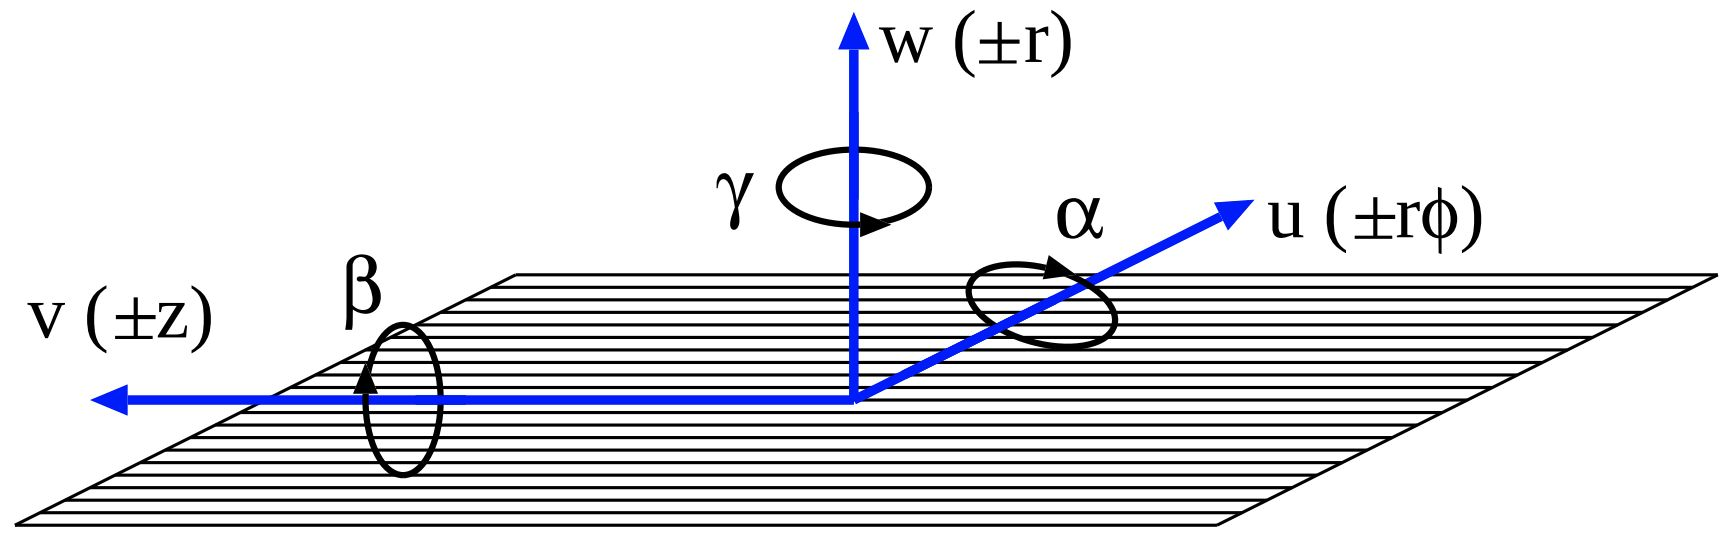
\includegraphics[width=0.8\textwidth,clip] {TrackerParam.jpg}
        \caption{Example local coordinates of a module. Global parameters are shown in parentheses for modules in the TIB and TOB \cite{WAdam_2009}.}
        \label{fig:TrackerParam}
    \end{center}
\end{figure}

Hit positions and impact points of a track are systematically displaced if the module position is not known correctly.

The difference in local module coordinates between these two quantities are the ``track-hit residuals'' \cite{Karimaki:926537}.

Modules are parameterized as seen in Fig.~\ref{fig:overlapHits}:
\begin{itemize}
    \item w axis is normal to the module
    \item u and v axes are in the plane
    \item u axis more sensitive to direction of measurement
    \item Angles $\alpha$, $\beta$, and $\gamma$ describe rotations around u, v, w respectively
\end{itemize}

Hierarchical systems:
\begin{itemize}
    \item \{r, g, q\} = coordinates in \{global, composite, local\} system
    \item \{R, G\} = rotations between global and \{local, composite\} system
\end{itemize}

\begin{figure}[!htb]
    \begin{center}
        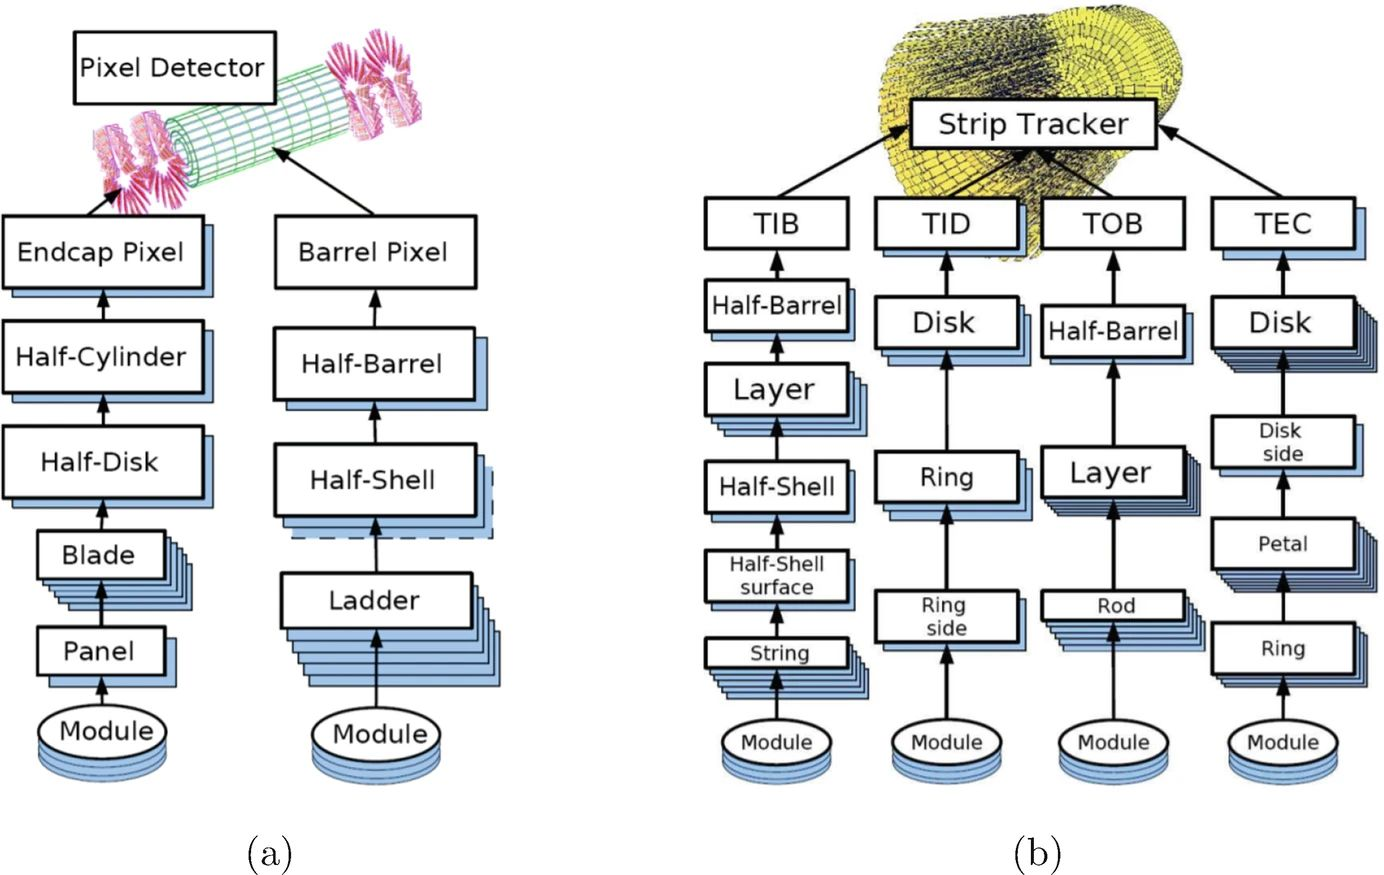
\includegraphics[width=0.8\textwidth,clip] {HLS.jpg}
        \caption{Diagrams of the hierarchical structures of the Pixel Detector and Strip Tracker \cite{WAdam_2009}.}
        \label{fig:HLS}
    \end{center}
\end{figure}

\subsection{Algorithms}

\begin{figure}[!htb]
    \begin{center}
        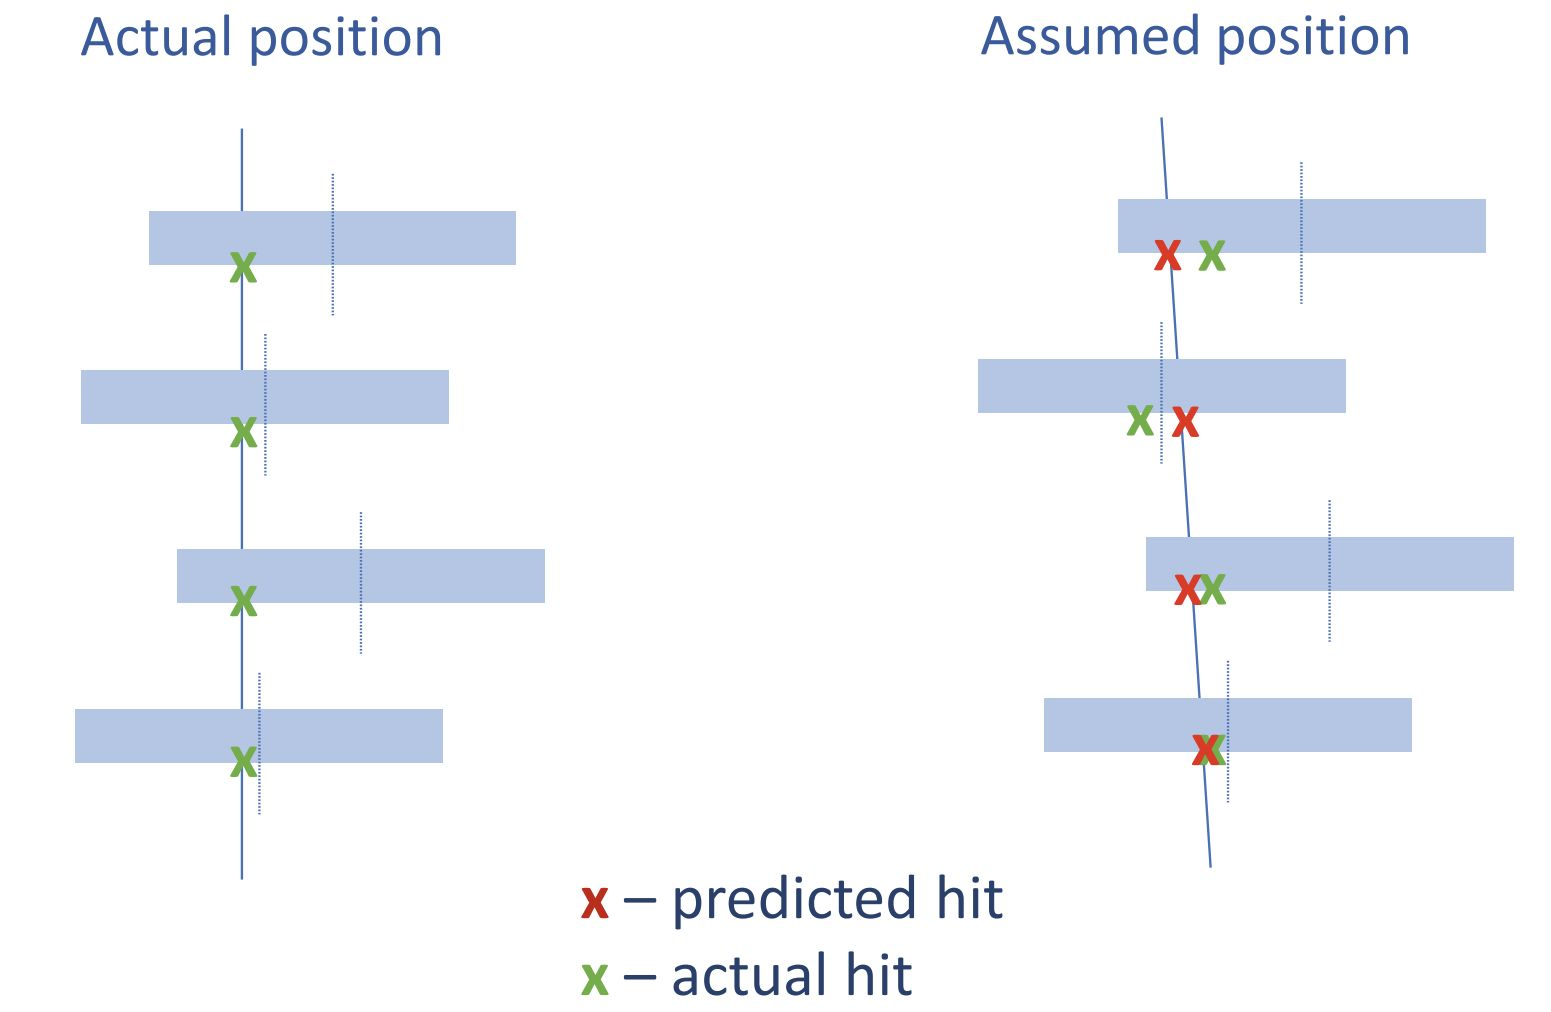
\includegraphics[width=0.8\textwidth,clip] {overlapHits.jpg}
        \caption{Simple illustration of a track through misaligned layers \cite{2022166795}.}
        \label{fig:overlapHits}
    \end{center}
\end{figure}

\subsubsection{MillePede}

% \begin{figure}[!htb]
%     \begin{center}
%         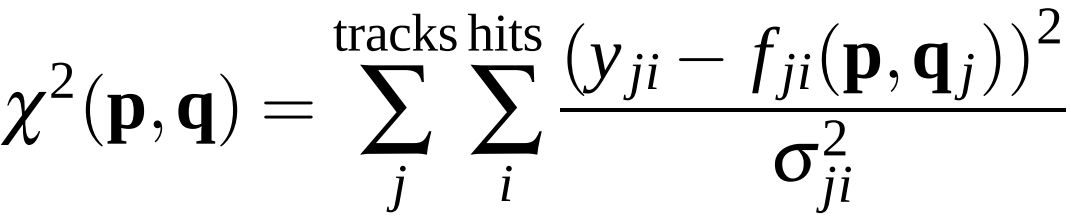
\includegraphics[width=0.8\textwidth,clip] {chi2MPiteration.jpg}
%         \caption{$\Xi^2$ function for MILLEPEDE-II global fit \cite{WAdam_2009}.}
%         \label{fig:chi2MPiteration}
%     \end{center}
% \end{figure}

\begin{equation}
\label{eq:MPX2}
\begin{gathered}
\mathcal{X} ^2 (p, q) = \Sigma_j^{tracks} \Sigma_i^{hits} \frac{(y_{ji} - f_{ji}(p, q_j))^2}{\sigma_{ji}^2}
\end{gathered}
\end{equation}

Unlike HipPy, MILLEPEDE-II (MP) opts to use a global matrix and forgoes the iterative approach.

\subsubsection{HipPy}

\begin{figure}[!htb]
    \begin{center}
        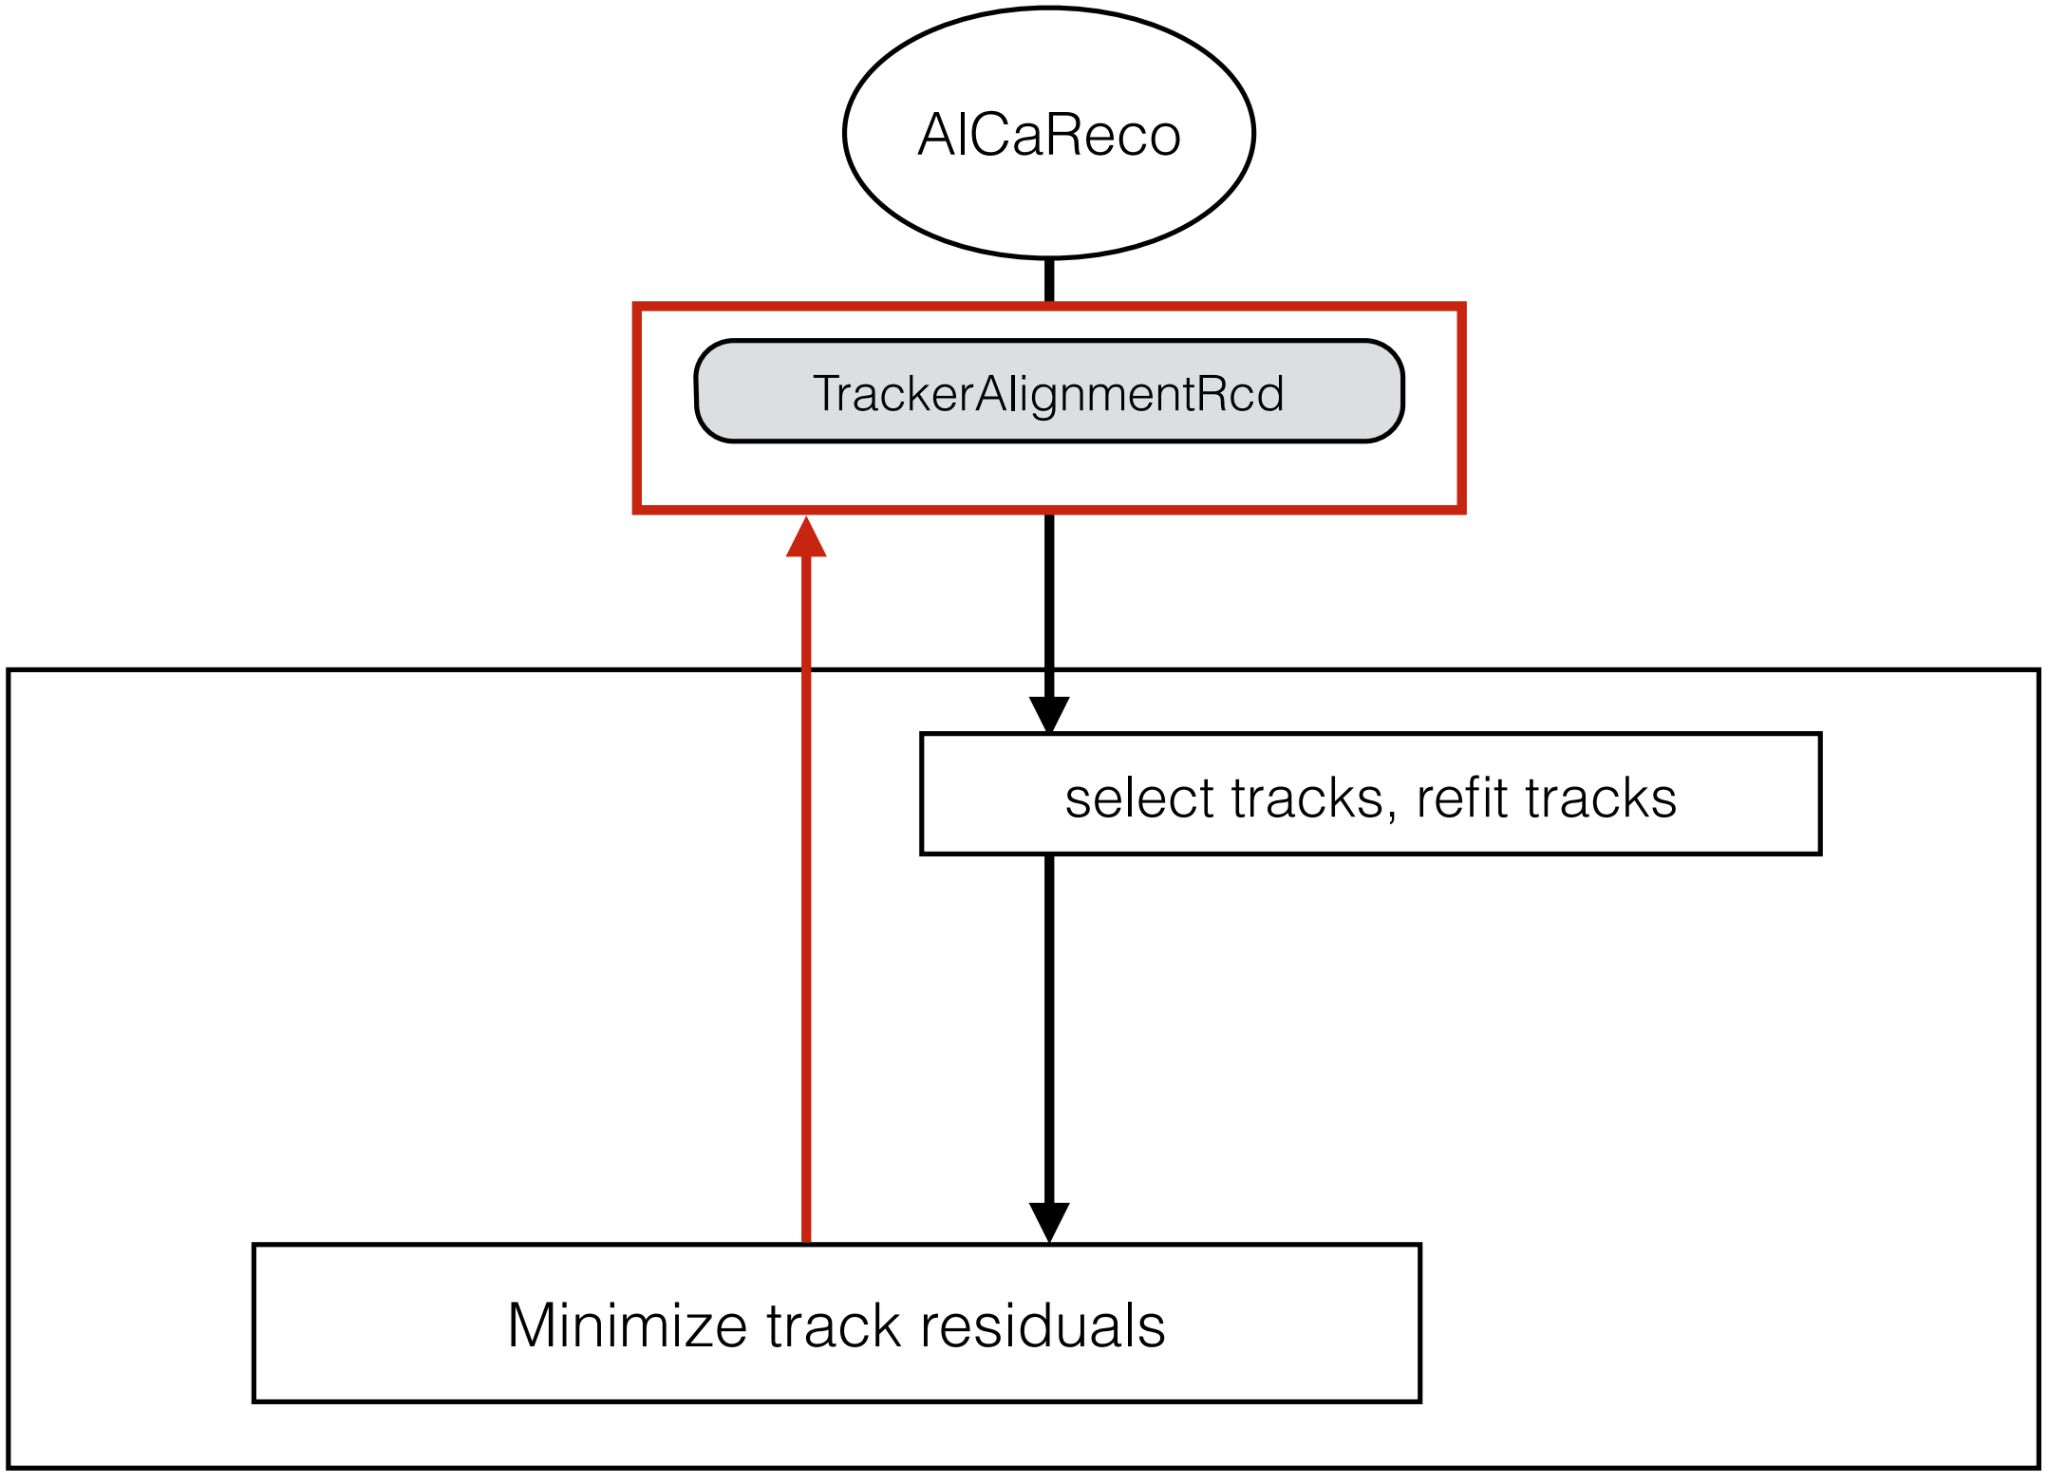
\includegraphics[width=0.8\textwidth,clip] {HIP.jpg}
        \caption{Process diagram of the Hits-and-Impact-Points (HIP) alignment algorithm \cite{2022166795}.}
        \label{fig:HIP}
    \end{center}
\end{figure}

\begin{figure}[!htb]
    \begin{center}
        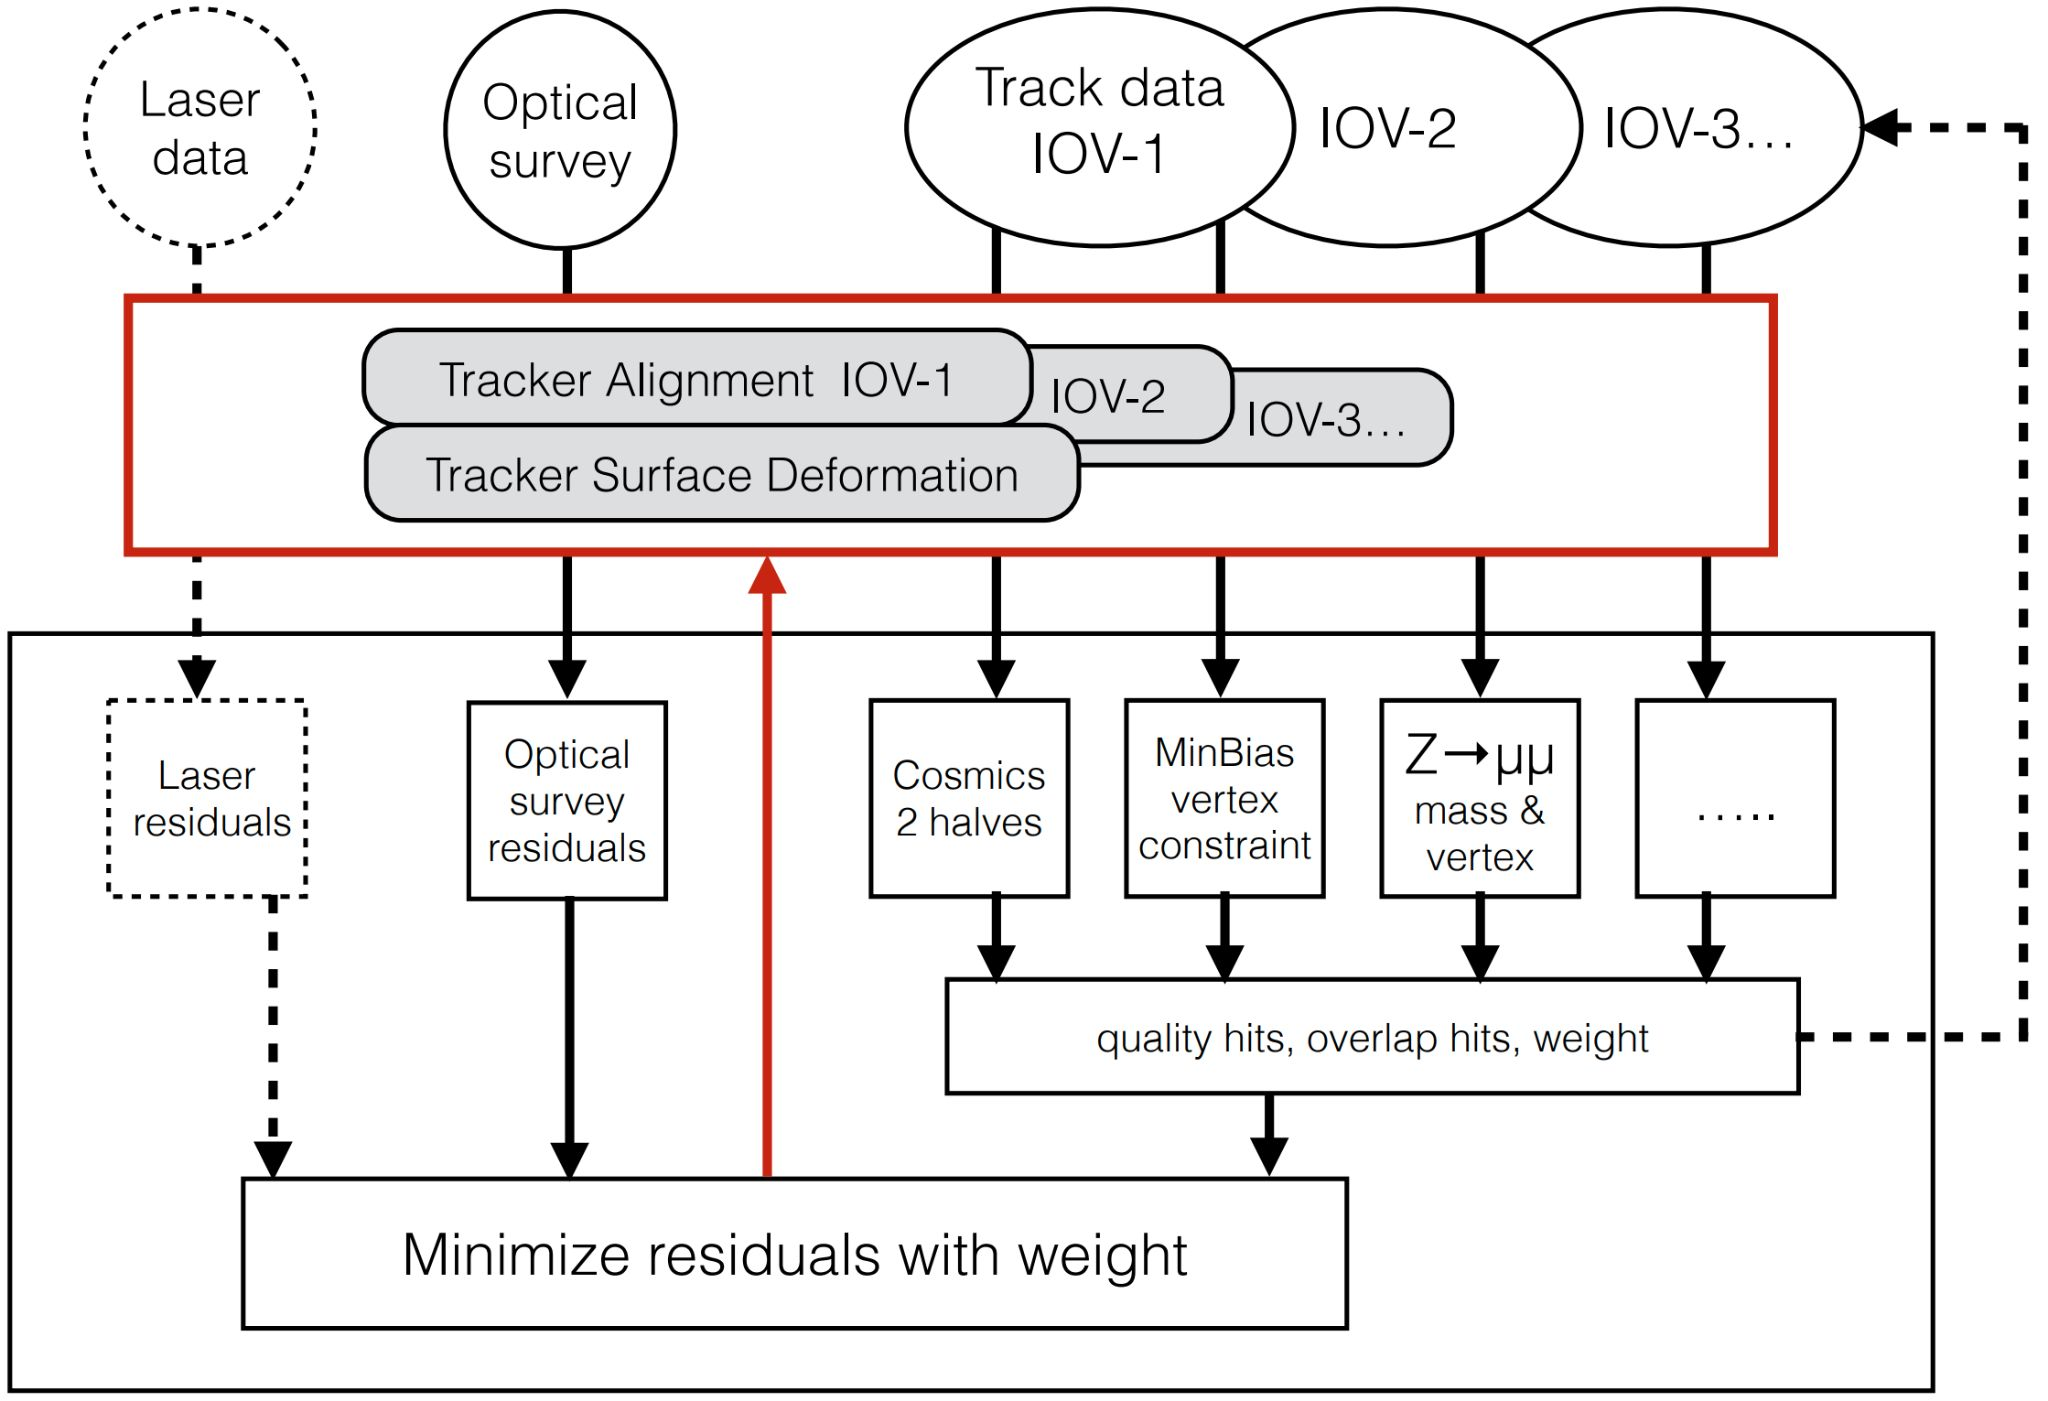
\includegraphics[width=0.8\textwidth,clip] {HipPy.jpg}
        \caption{Process diagram of the Hits-and-Impact-Points-Past-Year-1 (HipPy) alignment algorithm \cite{2022166795}.}
        \label{fig:HipPy}
    \end{center}
\end{figure}

% \begin{figure}[!htb]
%     \begin{center}
%         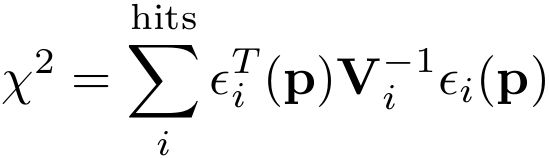
\includegraphics[width=0.8\textwidth,clip] {chi2HPiteration.jpg}
%         \caption{$\Xi^2$ function for HipPy fit.}
%         \label{fig:chi2HPiteration}
%     \end{center}
% \end{figure}

% \begin{figure}[!htb]
%     \begin{center}
%         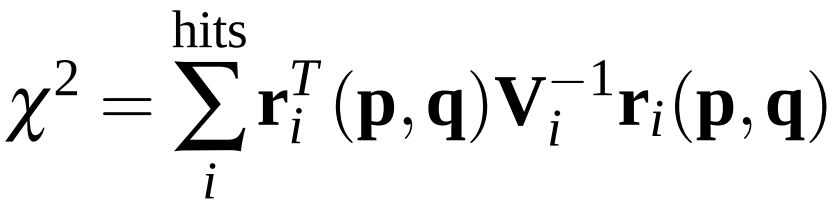
\includegraphics[width=0.8\textwidth,clip] {chi2HPiteration2.jpg}
%         \caption{$\Xi^2$ function for HipPy fit.}
%         \label{fig:chi2HPiteration2}
%     \end{center}
% \end{figure}

% \begin{figure}[!htb]
%     \begin{center}
%         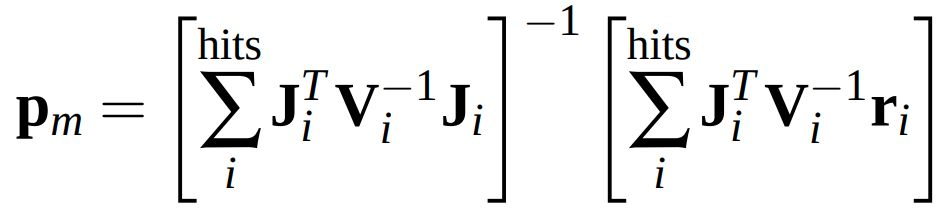
\includegraphics[width=0.8\textwidth,clip] {pmHPiteration.jpg}
%         \caption{Alignment parameters $p_m$ for HipPy fit.}
%         \label{fig:pmHPiteration}
%     \end{center}
% \end{figure}

The ``hits-and-impact-points'' (HIP) algorithm \cite{Karimaki:2003bd,Karimaki:926537} precedes what we now call HipPy.
Utilized during commissioning \cite{WAdam_2009} of the CMS tracker and for Run 1 \cite{CMSCollaboration_2010,Chatrchyan:1667597}.

Several notable features were added over time \cite{BROWN2009467} and the improved algorithm was renamed to “hits-and-impact-points-past-year-1” (HipPy) at the start of Run 2. 

Improvements to the alignment algorithm since Run 1:
\begin{itemize}
    \item The inclusion of 3 alignment parameters to describe sensor curvature (beyond the 6 position/orientation coordinates)
    \item The ability to weight certain types of input
    \item The option to perform sequential, hierarchical alignment over multiple time periods (multi-IOV)
    \item Optional mass and/or vertex constraints in certain types of events with known physics process
\end{itemize}

These features proved invaluable during Run 2, with successful HipPy-based alignment constants used in CMS data reconstruction (along with MP objects) in the prompt and EOY alignments\cite{BROWN2009467}.

The basic outline of the hits-and-impact-points (HIP) algorithm is as follows \cite{BROWN2009467}:
\begin{itemize}
    \item Load track data and hits
    \item The tracks are fit using the current estimate of the alignment parameters
    \item Hit $\mathcal{X} ^2$ are computed for the selected hits, following the definition in Eq.~\ref{eq:HIPX2}
    \item Minimize each sensor’s $\mathcal{X} ^2$ w.r.t. a change in only that sensor’s local alignment
    \item Hold the parameters of every other sensor fixed
    \item Calculate for every sensor
    \item Update the alignment parameters for all sensors with the computed change to the original estimate
    \item Use the updated local alignment to fit the tracks for the next iteration
    \item Repeat the process until the alignment converges
\end{itemize}

\begin{equation}
\label{eq:HIPX2}
\begin{gathered}
\mathcal{X} ^2 = \Sigma_i^{hits} \epsilon_i^T(p) V^{-1}_i \epsilon_i(p)
\end{gathered}
\end{equation}

\begin{itemize}
    \item HipPy leverages full integration of CMS software, which is helpful especially for track reconstruction
    \item Can make use of any constraint (e.g. mass, vertex) defined in that software
    \item Adds flexibility and simplifies development (e.g. Kalman filter)
    \item Position and orientation of each sensor are determined independently of other sensors in every iteration
    \item Multiple iterations are required to solve correlations between sensor parameters (requires multiple track fits)
    \item But each iteration is a straightforward application of a small matrix inversion
\end{itemize}

\begin{equation}
\label{eq:HPX2}
\begin{gathered}
\mathcal{X} ^2 = \Sigma_i^{hits} r_i^T(p, q) V^{-1}_i r_i(p, q)
\end{gathered}
\end{equation}

\begin{equation}
\label{eq:HPpm}
\begin{gathered}
p_m = [\Sigma_i^{hits} J^T_i V^{-1}_i J_i]^{-1} [\Sigma_i^{hits} J^T_i V^{-1}_i r_i]
\end{gathered}
\end{equation}

\begin{figure}[!htb]
    \begin{center}
        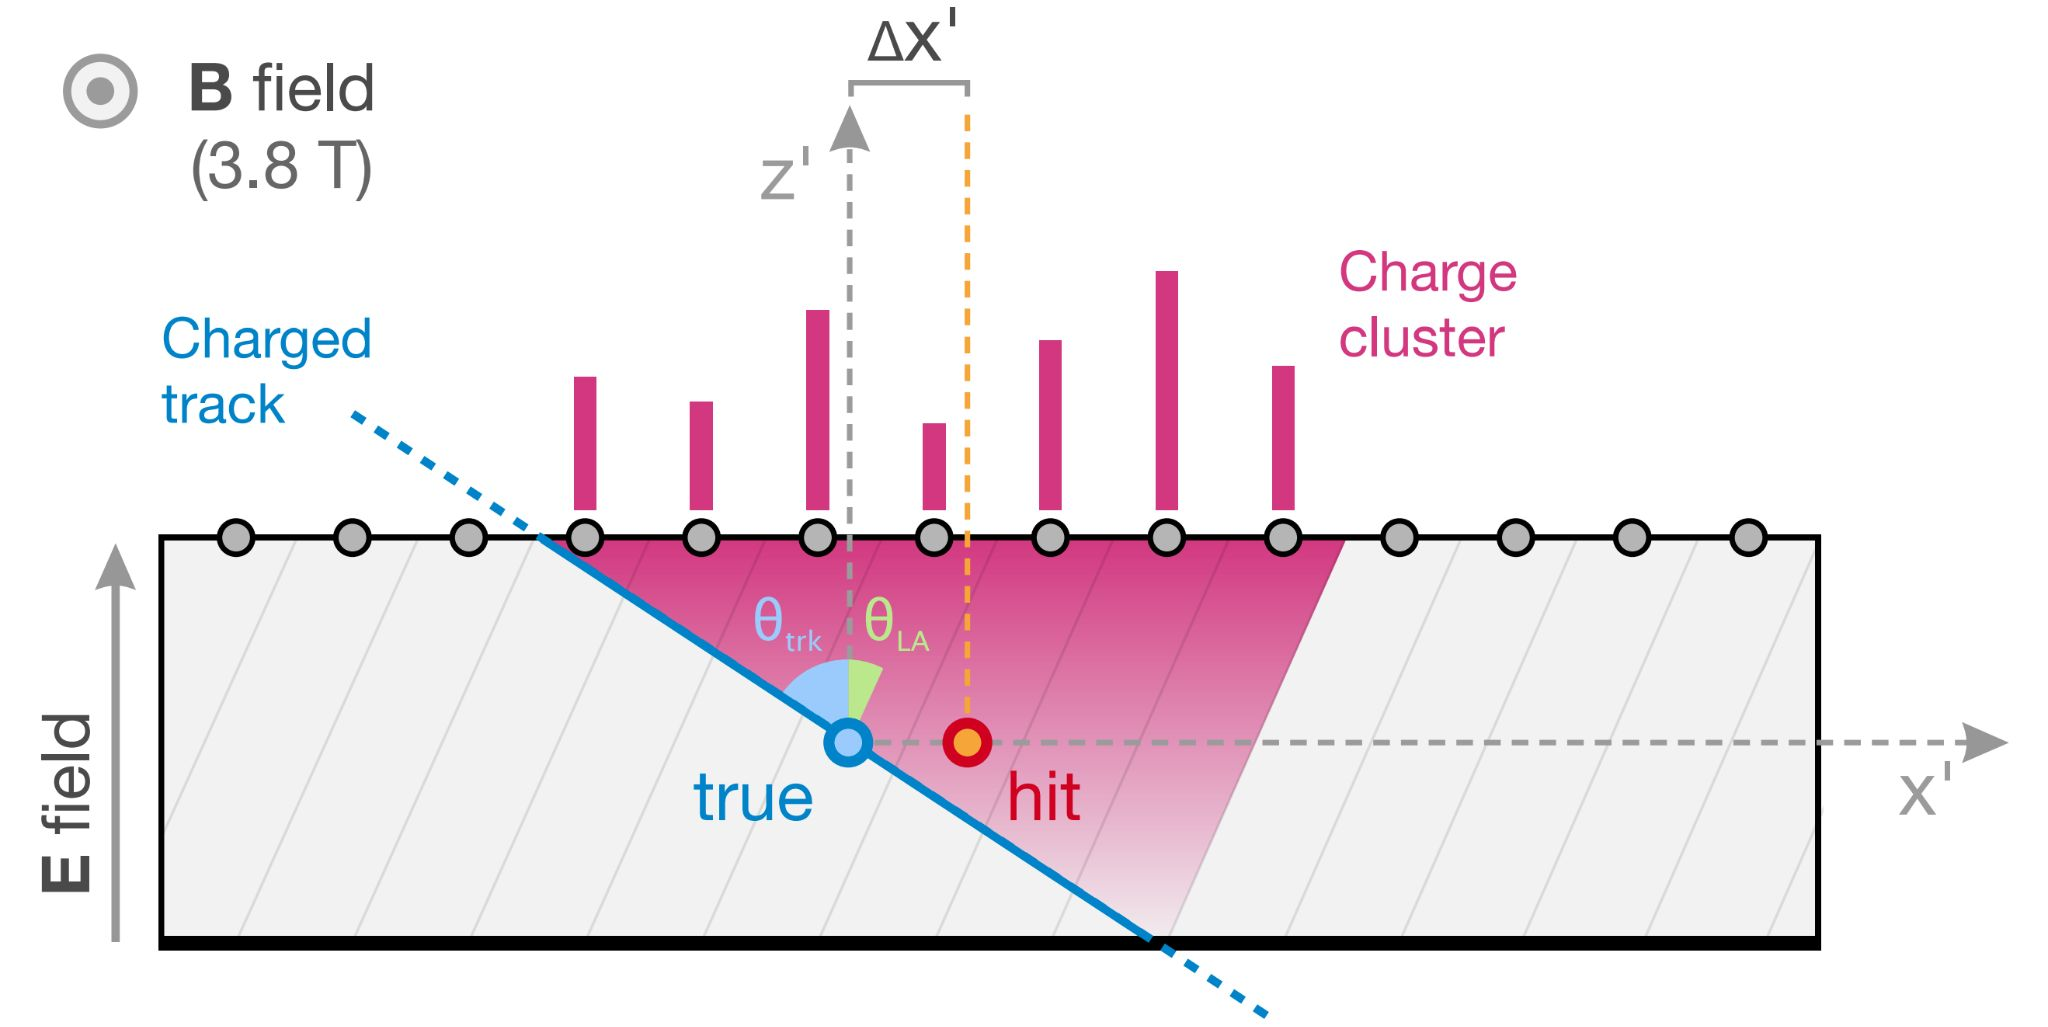
\includegraphics[width=0.8\textwidth,clip] {siliconmodule.jpg}
        \caption{Transverse view of a silicon module \cite{2022166795}.}
        \label{fig:siliconmodule}
    \end{center}
\end{figure}



\subsection{Validation}


\subsubsection{Geometry Comparison}


\subsubsection{Distribution of Median Residuals}


\subsubsection{Primary Vertex}


\subsubsection{Cosmic Track Splitting}


\subsubsection{Dimuon Validation}

$Z \rightarrow \mu\mu$


\chapter{Analysis of Higgs boson data at the LHC} \label{chap:chap-4}


% \begin{singlespace}
%     \epigraph{This is a large quote placed with \\ 
%     single spacing over two lines}{-- Unknown Author}
% \end{singlespace}


%% remove the following and add your chapter text here
% \section{A long section heading to test the distance before this}

% \blindtext

% \begin{figure}[ht]
% \begin{center}
%     \includegraphics[width=\textwidth, trim={6cm 5cm 6cm 5cm},clip,page=1] {chap4.pdf}
%     \caption{Here are some photos of ducks to make you feel happy in tough times.}
%     \label{fig:ducks}
% \end{center}
% \end{figure}

% \Blindtext[2]





% The SM postulates the existence of a Higgs field responsible for generating the masses of fundamental particles. The quantum excitation of this field is known as the Higgs boson ($H$)~\cite{StandardModel67_1, Englert:1964et, Higgs:1964ia, Higgs:1964pj, Guralnik:1964eu, StandardModel67_2, StandardModel67_3}. The properties of the \Hboson, observed with a mass of approximately 125\,GeV by the ATLAS and CMS Collaborations~\cite{Aad:2012tfa, Chatrchyan:2012xdj, Chatrchyan:2013lba} at the LHC, have been found to be consistent with the expectations of the SM~\cite{ATLASnature, CMSnature}. The mass of the \Hboson ($m_{H}$) is a free parameter of the model and, since it determines all other Higgs properties, should be measured with the highest possible precision. For instance, the Higgs boson’s couplings to vector bosons strongly depend on $m_H$ and are precisely predicted within the SM.

% Another critical property of the \Hboson is its lifetime, which is predicted in the SM to be $1.6\times10^{-22}$\,s, corresponding to a total width ($\Gamma_H$) of 4.1\,MeV~\cite{deFlorian:2016spz}, assuming $m_H = 125$\,GeV. Any deviation from this prediction would suggest the presence of anomalous Higgs couplings or decays into previously undetected particles. Hence, a precision measurement of the width ($\Gamma_H$) is valuable in the search for BSM physics. 

% The ATLAS and CMS Collaborations initially measured the \Hboson mass to be $125.09 \pm 0.24$\,GeV~\cite{Aad:2015zhl}, using $\sqrt{s} = 7$ and 8\,TeV proton-proton (pp) collision data from the 2011–2012 data-taking period (Run~1), corresponding to a total integrated luminosity of 25\,fb$^{-1}$ per experiment. This result has since been superseded by both experiments. The ATLAS Collaboration measured the \Hboson mass to be $125.11 \pm 0.11$\,GeV~\cite{ATLAS_mass}, combining the $H \to \gamma\gamma$ and $H \to 4\ell$ ($\ell = e$, $\mu$) channels from Run~1 and data collected at $\sqrt{s} = 13$\,TeV during 2015–2018 (Run~2). The value in parentheses indicates the statistical uncertainty only. The most recent CMS measurement, also using the $H \to \gamma\gamma$ and $H \to 4\ell$ channels and including Run~1 data together with 36\,fb$^{-1}$ of $\sqrt{s} = 13$\,TeV data from 2016, yields $m_{H} = 125.38 \pm 0.14$\,GeV, with a statistical uncertainty of 0.11\,GeV. Independent measurements using only the $H \to 4\ell$ channel and 2016 data report $m_H = 124.94 \pm 0.18$\,GeV (ATLAS) and $125.26 \pm 0.21$\,GeV (CMS), with statistical uncertainties of 0.17\,GeV and 0.19\,GeV, respectively.

% Assuming only on-shell Higgs boson production, CMS has set an upper limit on the \Hboson width of $\Gamma_H < 1.10$\,GeV at 95\% confidence level (CL), constrained by the four-lepton invariant mass resolution~\cite{Khachatryan:2014jba, Sirunyan:2017exp}. Both ATLAS and CMS have also constrained $\Gamma_H$~\cite{Khachatryan:2014iha, Aad:2015xua, Khachatryan:2015mma, Khachatryan:2016ctc, Aaboud:2018puo, Sirunyan:2019twz, CMS:2022ley} using an off-shell production method~\cite{Caola:2013yja, Kauer:2012hd, Campbell:2013una}, which relies on the measurement of the ratio of off-shell to on-shell production rates. Taking into account both gluon fusion (ggH) and electroweak (EW) production processes, the most recent results are $\Gamma_H = 3.2^{+2.4}_{-1.7}$\,MeV~\cite{CMS:2022ley} and $\Gamma_H = 4.3^{+3.3}_{-2.5}$\,MeV~\cite{atlascollaboration2023evidence}, reported by CMS and ATLAS, respectively. Furthermore, CMS has set a lower bound of $\Gamma_H > 3.5\times10^{-9}$\,MeV at 95\% CL, based on limits on the \Hboson flight distance in the detector~\cite{Khachatryan:2015mma}.

% In this chapter, I present an updated CMS measurement of the \Hboson width using off-shell production in the $H^* \to 4\ell$ decay channel. Additionally, I include results from a Higgs boson mass measurement conducted by collaborators using the shared on-shell data sample. The analysis is based on 138\,fb$^{-1}$ of $pp$ collision data at $\sqrt{s} = 13$\,TeV, collected from Run~2 between 2016 and 2018, combined with Run~1 data.

As previously discussed in Section~\ref{sec:higgs}, the SM postulates the existence of a scalar field---the Higgs field---responsible for the generation of mass for fundamental particles through the mechanism of electroweak symmetry breaking. The excitation of this field is known as the Higgs boson ($H$)~\cite{StandardModel67_1, Englert:1964et, Higgs:1964ia, Higgs:1964pj, Guralnik:1964eu, StandardModel67_2, StandardModel67_3}. The properties of the Higgs boson, observed with a mass of approximately 125\,GeV by the ATLAS and CMS Collaborations~\cite{Aad:2012tfa, Chatrchyan:2012xdj, Chatrchyan:2013lba} at the LHC, are found to be in agreement with SM predictions~\cite{ATLASnature, CMSnature}. 

The mass of the Higgs boson ($m_H$) is a free parameter in the SM and governs all other Higgs boson properties, necessitating its measurement with the highest possible precision. For instance, the Higgs boson couplings to vector bosons depend strongly on $m_H$ and are predicted with high precision within the SM framework. Another key parameter is the Higgs boson's total decay width ($\Gamma_H$), which determines its lifetime. The SM predicts a width of $\Gamma_H = 4.1$\,MeV, corresponding to a lifetime of $1.6 \times 10^{-22}$\,s~\cite{deFlorian:2016spz} for $m_H = 125$\,GeV. Any deviation from this prediction could signal anomalous Higgs boson couplings or decays to invisible or non-SM particles.

Using $\sqrt{s} = $7 and 8\,TeV proton-proton (pp) collision data collected during Run~1 (2011–2012), the ATLAS and CMS Collaborations jointly measured the Higgs boson mass as $125.09 \pm 0.24$\,GeV~\cite{Aad:2015zhl}, based on a combined integrated luminosity of 25\,fb$^{-1}$ per experiment. This result has since been superseded. The ATLAS Collaboration, combining the $H \to \gamma\gamma$ and $H \to 4\ell$ ($\ell = e, \mu$) decay channels using both Run~1 and Run~2 ($\sqrt{s} = 13$\,TeV, 2015–2018) data, reported a measurement of $m_H = 125.11 \pm 0.11\,\mathrm{GeV}$, with a statistical uncertainty of 0.09\,GeV~\cite{ATLAS_mass}. The most recent CMS result, using the same decay channels and including Run~1 and 36\,fb$^{-1}$ of 2016 data, yields $m_H = 125.38 \pm 0.14\,\mathrm{GeV}$, with a statistical uncertainty of 0.11\,GeV. Independent measurements from ATLAS and CMS based solely on the $H \to 4\ell$ decay and 2016 data give $m_H = 124.94 \pm 0.18 (\pm 0.17)$\,GeV and $m_H = 125.26 \pm 0.21 (\pm 0.19)$\,GeV, respectively, where the value in parentheses is the statistical uncertainty only.

Using only on-shell production, CMS placed an upper limit on the Higgs boson width of $\Gamma_H < 1.10$\,GeV at 95\% confidence level (CL), constrained by the four-lepton invariant mass resolution~\cite{Khachatryan:2014jba, Sirunyan:2017exp}. Both ATLAS and CMS have also set more stringent constraints using the off-shell production method~\cite{Khachatryan:2014iha, Aad:2015xua, Khachatryan:2015mma, Khachatryan:2016ctc, Aaboud:2018puo, Sirunyan:2019twz, CMS:2022ley}, which exploits the ratio of off-shell to on-shell production cross sections~\cite{Caola:2013yja, Kauer:2012hd, Campbell:2013una}. This method yields recent measurements of $\Gamma_H = 3.2^{+2.4}_{-1.7}$\,MeV by CMS~\cite{CMS:2022ley}, and $\Gamma_H = 4.3^{+3.3}_{-2.5}$\,MeV by ATLAS~\cite{atlascollaboration2023evidence}. Additionally, from limits on the Higgs boson's flight distance in the detector, CMS set a lower bound of $\Gamma_H > 3.5 \times 10^{-9}$\,MeV at 95\% CL~\cite{Khachatryan:2015mma}.

This chapter presents an updated CMS measurement of the \Hboson width using off-shell production in the $H^* \to 4\ell$ decay channel. Additionally, I include results from an extension of the off-shell analysis, as well as a Higgs boson mass measurement conducted by collaborators using the shared on-shell data sample. The analysis is based on 138\,fb$^{-1}$ of $pp$ collision data at $\sqrt{s} = 13$\,TeV, collected from Run~2 between 2016 and 2018, combined with Run~1 data.

% This thesis presents an updated CMS measurement of the Higgs boson width using off-shell production in the $H^* \to 4\ell$ decay channel. It also includes a mass measurement performed by collaborators using the same on-shell dataset. The analysis is based on a combined dataset of 138\,fb$^{-1}$ of $pp$ collision data at $\sqrt{s} = 13$\,TeV collected from 2016 to 2018, along with data from Run~1.







% The SM of particle physics postulates the existence of a Higgs field responsible for the
% generation of the masses of fundamental particles. The excitation of this
% field is known as the Higgs boson ($H$)~\cite{StandardModel67_1, Englert:1964et,Higgs:1964ia,
% Higgs:1964pj,Guralnik:1964eu,StandardModel67_2,StandardModel67_3}.
% The properties of the \Hboson, observed with a mass of approximately 125 GeV by the ATLAS and CMS
% Collaborations~\cite{Aad:2012tfa,Chatrchyan:2012xdj,Chatrchyan:2013lba} at the LHC, are found to be consistent with
% the expectations of the SM~\cite{ATLASnature,CMSnature}. The mass of the \Hboson ($m_{H}$) is a free parameter of the model and, since it determines all other Higgs properties, should be measured with as high precision as possible.
% For example, the Higgs boson couplings to vector bosons strongly depend on the \Hboson mass and are precisely predicted by the SM.
% Another important \Hboson characteristic is its lifetime, predicted by the SM to be $1.6\times10^{-22}$\,s, corresponding to a total width ($\Gamma_H$) of $4.1$ MeV~\cite{deFlorian:2016spz},
% as predicted precisely within the SM for $m_{H} = 125$ GeV.
% A deviation from the SM prediction would point to either anomalous \Hboson couplings or its decay to yet undiscovered particles.

% The ATLAS and CMS Collaborations measured the \Hboson mass to be $125.09 \pm 0.24$ GeV~\cite{Aad:2015zhl} using $\sqrt{s}=7$ and 8 TeV proton-proton (pp) collision data from the 2011--2012 data-taking periods (Run1), corresponding to a total integrated luminosity per experiment of 25 $fb^{-1}$.
% This result has been superseded by both collaborations.
% The ATLAS experiment measured the \Hboson mass to be $125.11 \pm 0.11 (\pm 0.09)$ GeV~\cite{ATLAS_mass}, combining the $H \to \gamma\gamma$ and $H \to 4\ell$ ($\ell = e$, $\mu$) channels from Run 1 and data collected at $\sqrt{s}=13$ TeV in 2015--2018 (Run~2).
% The value in parentheses is the statistical uncertainty only.
% The most recent CMS result, also using the $H \to \gamma\gamma$ and $H \to 4\ell$ channels and including Run 1 and 36 $fb^{-1}$ of $\sqrt{s}=13$ TeV data from 2016, is 
% $m_{H}$ = $125.38 \pm 0.14$ $(\pm 0.11)$ GeV.
% Measurements from ATLAS and CMS using only the $H \to 4\ell$ channel and 2016 data are $124.94 \pm 0.18 (\pm 0.17)$ GeV and $125.26 \pm 0.21 (\pm 0.19)$ GeV, respectively.

% Considering only on-shell Higgs boson production, CMS set an upper limit 
% on the \Hboson width $\Gamma_H < 1.10$ GeV at 95\% confidence level (CL), 
% limited by the four-lepton invariant mass resolution~\cite{Khachatryan:2014jba,Sirunyan:2017exp}.
% Both the ATLAS and CMS experiments have also set limits on 
% $\Gamma_H$~\cite{Khachatryan:2014iha,Aad:2015xua,Khachatryan:2015mma,
% Khachatryan:2016ctc,Aaboud:2018puo,Sirunyan:2019twz,CMS:2022ley}
% from an off-shell production method~\cite{Caola:2013yja,Kauer:2012hd,Campbell:2013una},
% which relies on the measurement of the ratio of off- to on-shell production rates.
% Considering both gluon fusion (ggH) and electroweak (EW) processes, the most recent measurements are
% $\Gamma_H= 3.2^{+2.4}_{-1.7}$ MeV~\cite{CMS:2022ley} and $\Gamma_H = 4.3^{+3.3}_{-2.5}$ MeV~\cite{atlascollaboration2023evidence} by CMS and ATLAS, respectively.
% Finally, from an upper limit on the \Hboson flight distance in the detector,
% CMS set a lower limit of $\Gamma_H > 3.5\times10^{-9}$ MeV at 95\% CL~\cite{Khachatryan:2015mma}.

% This thesis targets an updated CMS measurement of the \Hboson width using off-shell production and the $H^* \to 4\ell$ decay. I also include results of a Higgs boson mass measurement taken by our collaborators utilizing our shared on-shell statistics. The data sample includes 138 $fb^{-1}$ of $pp$ collision data at $\sqrt{s}=13$ TeV collected in 2016--2018, in combination with the Run 1 data.




% Compared to the previous CMS on-shell \Hboson measurement in this channel~\cite{Sirunyan:2017exp}, 
% the statistical and systematic uncertainties affecting $m_{H}$ have been reduced by including the beam spot in a refit of the muon tracks; 
% adopting an improved event categorization procedure; and performing a detailed study of the lepton momentum scale and resolution.








% A measurement of the relative off- and on-shell \Hboson production offers direct information about 
% \Gamma_H~\cite{Caola:2013yja,Kauer:2012hd,Campbell:2013una}.
% For each \Hboson production mechanism $j$, with subsequent decay to four leptons, 
% the on- and off-shell cross sections $\sigma_j$ are proportional to
% \begin{equation}
% 	\label{eq:resonant}
% 	\sigma_j^\text{on-shell} \propto \mu_j^\text{on-shell} 
% 	\quad\text{and}\quad
% 	\sigma_j^\text{off-shell} \propto \mu_j^\text{on-shell}  \ \Gamma_H,
% \end{equation}
% where $\mu_j^\text{on-shell}$ is the on-shell signal strength, defined as the ratio of the observed number of on-shell four-lepton events relative to the SM expectation.
% The signal strength is denoted as $\mu_F$ for \Hboson production mechanisms driven by fermion couplings, 
% \ie, production via ggH or in association with a t\bar{t} (\ttH) or \bbar pair (\bbH). 
% For EW production, \ie, production via vector boson fusion (VBF) 
% or in association with a $W$ or $Z$ boson (VH), the ratio is denoted as $\mu_V$.
% Contrary to gluon fusion and EW on-shell production, there is sizable destructive interference between 
% the \Hboson signal and the nonresonant four-lepton production in the off-shell region~\cite{Lee:1977yc,Kauer:2012hd}.
% This interference is crucial for maintaining unitarity and scales with $\sqrt{ \smash[b]{\mu_j^\text{on-shell} \Gamma_H}}$.

% In the described technique for measuring \Gamma_H, it is anticipated that the ratio of the couplings governing off- and on-shell 
% production production matches the SM prediction. 
% In particular, it is assumed that the dominant production mechanism is $ggH$ rather than quark-antiquark annihilation.
% The dominance of the $ggH$ production mechanism has been thoroughly tested in the on-shell regime~\cite{deFlorian:2016spz, CMSnature}. 
% It is also assumed that beyond-SM particles do not make significant contributions to the $ggH$ loop within the mass range considered by the analysis.
% In this paper, we explicitly test this assumption for the first time through a joint off- and on-shell analysis and find that the 
% \Gamma_H constraints are not substantially altered.
% In our previous off-shell analyses~\cite{Sirunyan:2019twz,CMS:2022ley}, we evaluated the anomalous contributions 
% to the $HVV$ vertex (where $V$ denotes a W boson, Z boson, or $gg$) in both EW production and \Hboson decay. 
% We found that these potential contributions did not significantly affect the \Gamma_H bounds.
% It is also assumed that no beyond-SM particles, such as higher-mass resonances, significantly contribute within the mass range 
% investigated by the analysis. However, such resonances would typically increase the yield of events at higher masses, 
% which is not supported by our measurement, and no such resonances have been found in a direct search~\cite{Sirunyan:2018qlb}.
% These tests do not address every possible scenario that could impact the measurement of the width, but
% a violation of any of the above assumptions would, by itself, indicate the presence of physics beyond the SM.

% The \Hboson width may deviate from the SM expectation of 4.1\MeV~\cite{deFlorian:2016spz}
% if the \Hboson has non-SM decay channels, or if the known decay modes have non-SM rates. 
% Therefore, the direct measurement of the \Hboson width complements searches for \Hboson decays to invisible 
% or undetected particles and measurements of the \Hboson couplings to the known SM particles.
% For example, if the Higgs boson decays into a pair of unknown particles, potentially candidates 
% for dark matter, this would increase the predicted Higgs boson width but 
% would not introduce a bias into the measurement techniques used in the current analysis. 


%\subsection{Full Run 2 Analysis}

%\subsection{Combined Run 1 and Run 2 Analysis}

\section{Modeling of off-shell production}

% In this subsection, we provide more technical details on the MC samples used in this analysis.

This analysis takes advantage of new tools for off-shell simulation that are now available through JHUGen \cite{2010,2012,2014,2016,2020,2021}. With the release of JHUGen v7.2.4, options were added to generate off-shell EW events, including hadronic VH production, the continuum background, and up to two scalar resonances. By release v7.3.0, the generation of interference in $4\ell$ final states in off-shell EW production was improved and we were able to simulate off-shell EW Higgs boson production with the inclusion of the anomalous couplings described in Section~\ref{sec:amplitudeEFT}. In conjunction with the previously available simulations for off-shell gluon fusion production, illustrated in Figure~\ref{fig:offshellAC_BSI}, this enables us to perform future off-shell analysis of these anomalous couplings with all primary Higgs boson production modes simulated through JHUGen. When we incorporate anomalous couplings into future analyses, reweighting techniques will also allow us to create distributions for hypotheses with mixed anomalous contributions to the HVV amplitude. This significantly reduces the number of unique samples we must generate. 
% This significantly reduces the number of uniquely generated samples we need to produce. 

\begin{figure}[!hbt]
\centering
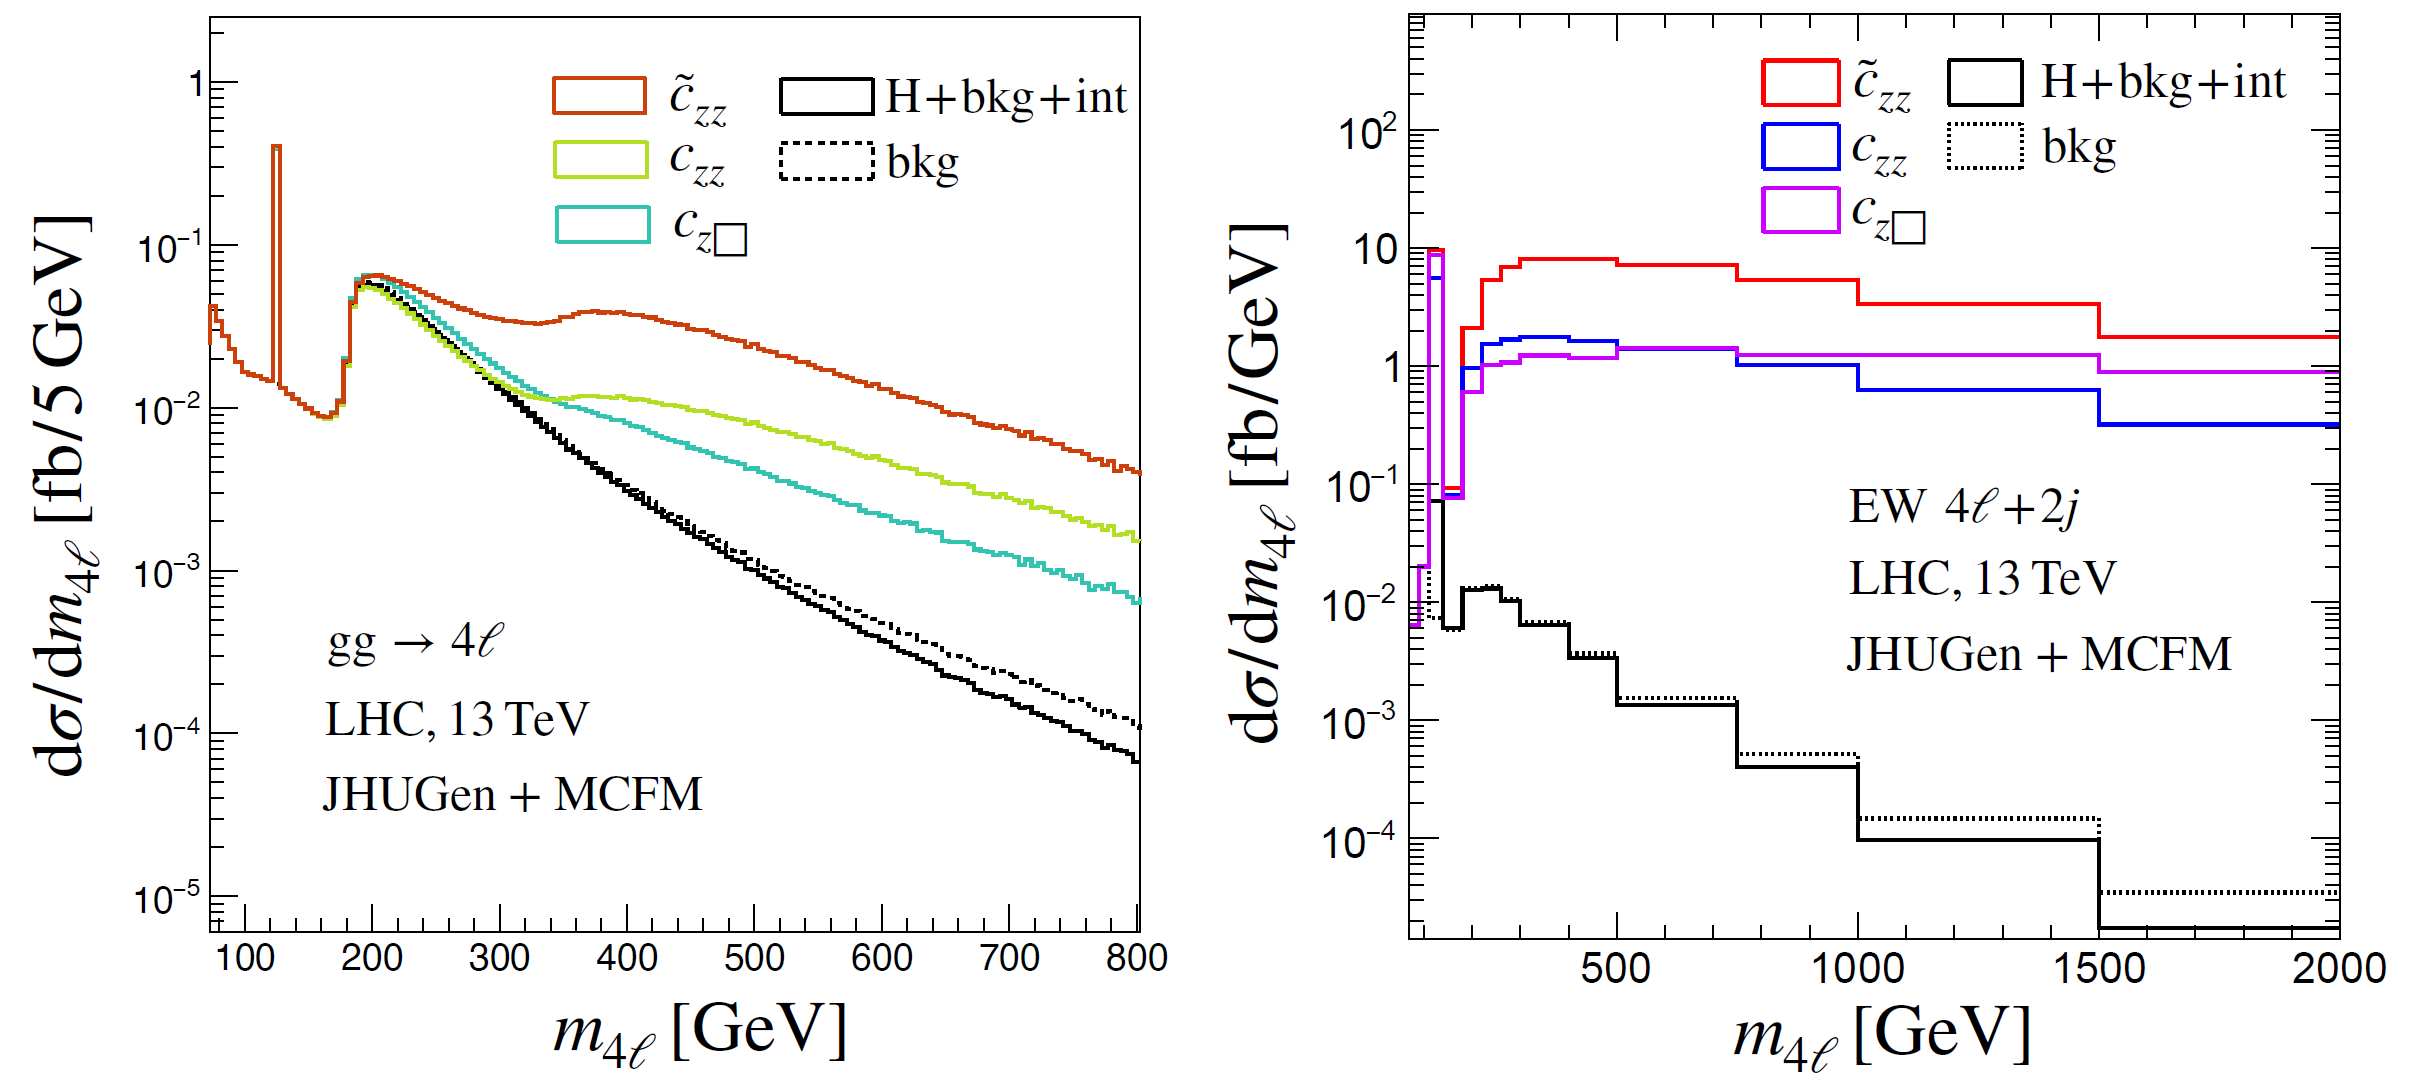
\includegraphics[width=0.9\textwidth,clip] {figures/offshellAC_BSI.png}
\caption{ The four-lepton $m_{4\ell}$ invariant mass distributions for gluon fusion (left) and electroweak production in association with two jets (right) at the LHC with a 13 TeV pp collision energy. The total SM production (“H+bkg+int”) and background-only (“bkg”) components are shown in black. Three operators $c_z$ (magenta), $c_{zz}$ (blue), and $\tilde{c}_{zz}$ (red) are shown in color, as analogs of the anomalous couplings described in Section~\ref{sec:amplitudeEFT}, and they are introduced in place of the SM interaction with their strength constrained to reproduce the SM cross section of the on-shell Higgs boson signal production \cite{offshellWGnote}.}
\label{fig:offshellAC_BSI}
\end{figure}

Notably, as is done in this analysis, we can also reweight these various samples to the same SM-like hypothesis, and leverage the additional statistics to make a more precise measurement of the SM-like Higgs boson. The matrix element likelihood approach (MELA), which I will discuss further in Section~\ref{sec:mela}, is used to reweight all simulated off-shell events to the SM hypothesis through modified MCFM matrix elements \cite{12077235,10073492}. This eliminates the need for out-of-the-box simulation of additional SM events by utilizing statistics from our pre-existing BSM simulations instead. Furthermore, this analysis improves on past papers \cite{190100174} by including the entire Run 2 dataset (spanning years 2016, 2017, and 2018). Table~\ref{tab:samplesDAStable} provides an accounting of the datasets used.

\begin{table}[!hbt]
	\centering
	\resizebox{\textwidth}{!}{%
		\begin{tabular}{|l|l|}
			\hline
			Process         & Dataset Name      \\ \hline
			$gg \to H \to ZZ \to 4\ell$            & /GluGluToHiggs*ToZZTo*\_M125\_GaSM*\_13TeV\_MCFM701\_pythia8/ \\ 
			$q\bar{q} \to Hqq \to ZZqq \to 4\ell qq$    & /VBFToHiggs0*ToZZTo4l\_M125\_GaSM\_13TeV\_JHUGenV730\_MCFM701\_pythia8/ \\ 
			$q\bar{q} \to W^{\pm}H \to ZZZ\to 4\ell + X$    & /VBFToHiggs0*ToZZTo4l\_M125\_GaSM\_13TeV\_JHUGenV730\_MCFM701\_pythia8/ \\ 
			$q\bar{q} \to ZH \to ZZZ \to 4\ell + X$    & /VBFToHiggs0*ToZZTo4l\_M125\_GaSM\_13TeV\_JHUGenV730\_MCFM701\_pythia8/ \\ \hline
			
			$gg \to H \to ZZ \to 4\ell$            & /GluGluHToZZTo4L\_M*\_13TeV\_powheg2\_JHUGenV7011\_pythia8/ \\ 
			$q\bar{q} \to Hqq \to ZZqq \to 4\ell qq$    & /VBF\_HToZZTo4L\_M*\_13TeV\_powheg2\_JHUGenV7011\_pythia8/ \\
			$q\bar{q} \to W^{+}H \to ZZZ\to 4\ell + X$    &  /WplusH\_HToZZTo4L\_M*\_13TeV\_powheg2-minlo-HWJ\_JHUGenV7011\_pythia8/\\ 
			$q\bar{q} \to W^{-}H \to ZZZ\to 4\ell + X$    &  /WminusH\_HToZZTo4L\_M*\_13TeV\_powheg2-minlo-HWJ\_JHUGenV7011\_pythia8/\\ 
			$q\bar{q} \to ZH \to ZZZ \to 4\ell + X$    & /ZH\_HToZZ\_4LFilter\_M*\_13TeV\_powheg2-minlo-HZJ\_JHUGenV7011\_pythia8/ \\ 
			$t\bar{t} \to H \to ZZ \to 4\ell$    & 	/ttH\_HToZZ\_4LFilter\_M*\_13TeV\_powheg2\_JHUGenV7011\_pythia8/ \\ \hline
			
			$q\bar{q} \to Hqq \to ZZqq \to 4\ell qq$    & /VBFToHiggs0PMContinToZZTo*JJ\_M125\_GaSM\_13TeV\_phantom\_pythia8/ \\ 
			$q\bar{q} \to Hqq \to ZZqq \to 4\ell qq$    & /ZZJJTo4L\_EWK\_TuneCP5\_13TeV-madgraph-pythia8/ \\ \hline
			
			$gg \to H \to ZZ \to 4\ell$            & /Higgs0PMToZZTo4L\_M125\_13TeV\_powheg2\_JHUGenV7011\_pythia8/ \\ 
			$q\bar{q} \to Hqq \to ZZqq \to 4\ell qq$    & /VBFHiggs0PMToZZTo4L\_M125\_13TeV\_JHUGenV7011\_pythia8/ \\ 
			$q\bar{q} \to W^{\pm}H \to ZZZ\to 4\ell + X$    & /WHiggs0PMToZZTo4L\_M125\_13TeV\_JHUGenV7011\_pythia8/ \\ 
			$q\bar{q} \to ZH \to ZZZ \to 4\ell + X$    & /ZHiggs0PMToZZ\_4LFilter\_M125\_13TeV\_JHUGenV7011\_pythia8/ \\ \hline
			
			$qq \to ZZ \to 4\ell$                           & /ZZTo4L\_13TeV\_powheg\_pythia8/ \\ \hline
		\end{tabular}%
	}
	\caption{Table of datasets used for Higgs boson production and $ZZ \to 4\ell$ decay modes.}
	\label{tab:samplesDAStable}
\end{table}

% Here, we have documented inputs used to generate samples that include on-shell events. 
There already exist on-shell samples (centered around the 125 GeV Higgs boson peak) for our dominant production modes generated with POWHEG v2 and JHUGen v7.0.11, which have been validated and utilized in CMS analyses~\cite{Sirunyan:2019twz, Sirunyan:2021rug, Sirunyan:2765059} so we can inherit them to use for our on-shell Higgs boson cross-section, and as a reliable point of comparison for newly generated MC events. We also have as additional samples for electroweak production, on-shell samples generated with JHUGen+JHUGenMELA and off-shell samples of the combined BSI (background+signal+interference) events via Phantom.

These samples are valuable in the validation of the recently produced off-shell samples for gluon fusion and electroweak production, which were generated using JHUGen v7.3.0 interfaced to MCFM v7.0.1 and MCFM v7.0.6. It is important to note here, as we compare on-shell events between all these samples using the cross-section and branching ratio values from Yellow Report (YR) 4, that the off-shell samples share common generator inputs which are not applied to the on-shell samples~\cite{YellowRep4}. These cuts and their associated efficiencies are documented in Table~\ref{tab:geninputtable}.

\begin{table}[!hbt]
	\centering
	\resizebox{\textwidth}{!}{%
		\begin{tabular}{|c|c|c|c|}
			\hline
			Generator           &Sample / Analysis          & Leptons                   & Jets                                \\ \hline
			{JHUGen+MCFM}         &EW off-shell & $pT$ $l_{1,2,3,4} > 3 GeV$, $|\eta$ $l_{1,2,3,4}| < 2.7$ & $pT$ $j_{1,2} >$ 15 GeV, $m_{jj} > $30 GeV, $|\eta$ $j_{1,2}| <$ 6.5, $\Delta R$ $>$ 0.3, $|\Delta\eta$ $j_{1,2}| >$0 \\  
			
			&ggH off-shell  & $pT$ $l_{1,2,3,4} > 3 GeV$, $|\eta$ $l_{1,2,3,4}| < 2.7$ & $pT$ $j_{1,2} >$ 15 GeV, $\Delta R$ $>$ 0.4                   \\ \hline
			
			Phantom         &EW off-shell (BSI, $4e$) & $pT$ $l_{1,2,3,4} >$ 3 GeV, $|\eta$ $l_{1,2,3,4}| < 2.7$ & $m_{jj} > $30 GeV, $|\eta$ $j_{1,2}| <$ 6.5            \\ 
			&EW off-shell (BSI, $4\mu$) & $pT$ $l_{1,2,3,4} >$ 3 GeV, $|\eta$ $l_{1,2,3,4}| < 2.7$ & $m_{jj} > $30 GeV, $|\eta$ $j_{1,2}| <$  6.5            \\ 
			&EW off-shell (BSI, $2e2\mu$) & $pT$ $l_{1,2,3,4} >$ 3 GeV, $|\eta$ $l_{1,2,3,4}| < 2.7$ & $m_{jj} > $30 GeV, $|\eta$ $j_{1,2}| <$ 6.5            \\ \hline
			
			POWHEG+JHUGen                &VBF on-shell  & No specified cuts         & No specified cuts                   \\ 
			&W$^{-}$H on-shell  & No specified cuts         & No specified cuts                   \\ 
			&W$^{+}$H on-shell  & No specified cuts         & No specified cuts                   \\ 
			&ZH on-shell  & No specified cuts         & No specified cuts                   \\ 
			&ggH on-shell & No specified cuts         & No specified cuts                   \\ \hline
			
			JHUGen+JHUGen           &VBF on-shell         & No specified cuts         & $pT$ $j_{1,2} > 0$ GeV, $\Delta R > 0$ \\ 
			&WH on-shell         & No specified cuts         & No specified cuts \\ 
			&ZH on-shell         & No specified cuts         & No specified cuts \\ \hline
			
		\end{tabular}%
	}
	\caption{Generator-level cuts on jets and leptons in all utilized samples.}
	\label{tab:geninputtable}
\end{table}


% \begin{table}[h]
% 	\centering
% 	\resizebox{\textwidth}{!}{%
% 		\begin{tabular}{|c|c|c|c|}
% 			\hline
% 			Generator           &Sample / Analysis          & Leptons                   & Jets                                \\ \hline
% 			{JHUGen+MCFM}         &EW off-shell & $pT$ $l_{1,2,3,4} > 3 GeV$, $|\eta$ $l_{1,2,3,4}| < 2.7$ & $pT$ $j_{1,2} >$ 15 GeV, $m_{jj} > $30 GeV, $|\eta$ $j_{1,2}| <$ 6.5, $\Delta R$ $>$ 0.3, $|\Delta\eta$ $j_{1,2}| >$0, $sgn(\eta$ $j_{1}) = \pm sgn(\eta$ $j_{2})$ \\  
			
% 			&ggH off-shell  & $pT$ $l_{1,2,3,4} > 3 GeV$, $|\eta$ $l_{1,2,3,4}| < 2.7$ & $pT$ $j_{1,2} >$ 15 GeV, $\Delta R$ $>$ 0.4                   \\ \hline
			
% 			POWHEG+JHUGen                &VBF on-shell  & No specified cuts         & No specified cuts                   \\ 
% 			&W$^{-}$H on-shell  & No specified cuts         & No specified cuts                   \\ 
% 			&W$^{+}$H on-shell  & No specified cuts         & No specified cuts                   \\ 
% 			&ZH on-shell  & No specified cuts         & No specified cuts                   \\ 
% 			&ggH on-shell & No specified cuts         & No specified cuts                   \\ \hline
			
% 			JHUGen+JHUGen           &VBF on-shell         & No specified cuts         & $pT$ $j_{1,2} > 0$ GeV, $\Delta R > 0$ \\ 
% 			&WH on-shell         & No specified cuts         & No specified cuts \\ 
% 			&ZH on-shell         & No specified cuts         & No specified cuts \\ \hline
			
% 			Phantom         &EW off-shell (BSI, $4e$) & $pT$ $l_{1,2,3,4} >$ 3 GeV, $|\eta$ $l_{1,2,3,4}| < 2.7$ & $m_{jj} > $30 GeV, $|\eta$ $j_{1,2}| <$ 6.5            \\ 
% 			&EW off-shell (BSI, $4\mu$) & $pT$ $l_{1,2,3,4} >$ 3 GeV, $|\eta$ $l_{1,2,3,4}| < 2.7$ & $m_{jj} > $30 GeV, $|\eta$ $j_{1,2}| <$  6.5            \\ 
% 			&EW off-shell (BSI, $2e2\mu$) & $pT$ $l_{1,2,3,4} >$ 3 GeV, $|\eta$ $l_{1,2,3,4}| < 2.7$ & $m_{jj} > $30 GeV, $|\eta$ $j_{1,2}| <$ 6.5            \\ \hline
			
% 		\end{tabular}%
% 	}
% 	\caption{Table of generator-level cuts on jets and leptons in JHUGen off-shell samples.}
% 	\label{tab:geninputtable}
% \end{table}

Generator-level cuts are applied on leptons during the generation of the samples.
These selection cuts remove leptons that fall outside the detector acceptance or reconstruction capabilities. It has been validated that no leptons which would otherwise be reconstructed in the analysis are lost due to these cuts. However, it is important to evaluate their efficiency to ensure proper normalization of the cross sections. The impact of these cuts is assessed through independent Monte Carlo (MC) studies, where various processes are generated both with and without the aforementioned lepton selection. 

In the case of gluons fusion \offshell samples, only lepton selection requirements are applied:
\noindent $p_T(\ell_{1,2,3,4})> 3$ GeV, $|\eta(\ell_{1,2,3,4})| < 2.7$.
The effect of these cuts on inclusive samples, generated with JHUGen signal only, 
is shown in Table~\ref{tab:ggHlepteff}.

\begin{table}[!hbt]
\begin{center}
\begin{tabular}{|c|c|c|}
\hline
$m_H$ & H $\rightarrow$ $4e$ & H $\rightarrow$ $2e2\mu$ \\ 
\hline
125 GeV  & 64.413\%           & 64.285\%              \\ 
200 GeV  & 73.627\%           & 73.789\%              \\ 
300 GeV  & 78.098\%           & 78.061\%              \\ 
400 GeV  & 82.115\%           & 82.285\%              \\ 
500 GeV  & 85.217\%           & 85.214\%              \\ 
600 GeV  & 87.699\%           & 87.655\%              \\ 
\hline
\end{tabular}
\caption{
Efficiencies of generator-level requirements on leptons ($p_T(\ell_{1,2,3,4})> 3$ GeV, $|\eta(\ell_{1,2,3,4})| < 2.7$)
in the \offshell gluons fusion samples as a function of $m_{4\ell}$.
}
\label{tab:ggHlepteff}
\end{center}
\end{table}



In the case of EW \offshell samples, we evaluate efficiency of the generator-level cuts separately for
the VBF, WH, and ZH samples, and then combine them according to their relative cross sections, used as weight. 
First we evaluate effect of lepton selection requirements are applied:
\noindent $p_T(\ell_{1,2,3,4})> 3$ GeV, $|\eta(\ell_{1,2,3,4})| < 2.7$.
The effect of these cuts on EW samples, generated with JHUGen signal only, 
is shown in Table~\ref{tab:EWlepteff}.
The effect of jet cuts on EW samples, generated with JHUGen signal only, 
is shown in Table~\ref{tab:EWjeteff}.

\begin{table}[!hbt]
\begin{center}
\small
\begin{tabular}{|c|c|c|c|c|c|}
\hline
$m_H$ & VBF & WH  & ZH  & EW (had) & EW (full) \\ 
\hline
125 GeV  & 71.35\%    & 61.64\%    & 63.09\%    & 69.15\%     & 68.45\%              \\ 
200 GeV  & 78.90\%    & 71.45\%    & 72.18\%    & 78.13\%     & 77.83\%              \\ 
300 GeV  & 81.70\%    & 76.78\%    & 77.39\%    & 81.46\%     & 81.36\%              \\ 
400 GeV  & 84.57\%    & 82.06\%    & 82.46\%    & 84.50\%     & 84.47\%              \\  
500 GeV  & 86.95\%    & 85.77\%    & 85.91\%    & 86.93\%     & 86.92\%               \\  
600 GeV  & 88.72\%    & 88.19\%    & 88.28\%    & 88.71\%     & 88.71\%               \\  
\hline
\end{tabular}
\caption{
Efficiencies of generator-level requirements on leptons ($p_T(\ell_{1,2,3,4})> 3$ GeV, $|\eta(\ell_{1,2,3,4})| < 2.7$)
in the \offshell EW samples as a function of $m_{4\ell}$.
The EW (had) includes VBF and hadronic VH production, 
while EW (full) also includes leptonic VH production. 
}
\label{tab:EWlepteff}
\end{center}
\end{table}

\begin{table}[!hbt]
\begin{center}
\small
\begin{tabular}{|c|c|c|c|c|c|c|c|}
\hline
\multicolumn{1}{|c}{~} & \multicolumn{5}{|c|}{efficiency of jet cuts} & \multicolumn{2}{c|}{jet + lepton cuts} \\
\hline
$m_H$ & VBF & WH  & ZH  & EW (had) & EW (full)   & EW (had) & EW (full)          \\ 
\hline
125 GeV  & 86.92\%    & 85.49\%    & 88.38\%    & 86.84\%     & 86.81\%     & 60.05\%     & 59.42\%              \\ 
200 GeV  & 87.09\%    & 88.59\%    & 90.34\%    & 87.33\%     & 87.42\%     & 68.23\%     & 68.03\%             \\ 
300 GeV  & 87.28\%    & 91.50\%    & 92.48\%    & 87.51\%     & 87.61\%     & 71.29\%     & 71.28\%             \\ 
400 GeV  & 87.20\%    & 93.38\%    & 94.00\%    & 87.39\%     & 87.47\%     & 73.84\%     & 73.88\%             \\  
500 GeV  & 86.84\%    & 94.71\%    & 94.98\%    & 87.00\%     & 87.07\%     & 75.62\%     & 75.67\%              \\  
600 GeV  & 86.56\%    & 95.61\%    & 95.83\%    & 86.69\%     & 86.92\%     & 76.90\%     & 76.95\%              \\  
\hline
\end{tabular}
\caption{
Efficiencies of generator-level requirements on jets in the \offshell EW samples as a function of $m_{4\ell}$.
The EW (had) includes VBF and hadronic VH production, while EW (full) also includes leptonic VH production. 
These efficiencies are calculated after generator-level requirements had been applied on leptons,
as indicated in Table~\ref{tab:EWlepteff}.
The last two columns incorporate efficiency of lepton cuts together with jet cuts. 
}
\label{tab:EWjeteff}
\end{center}
\end{table}


\subsection{$K$ factors}

\subsubsection{ggH processes}

The cross section for the SM Higgs boson produced via gluon fusion in the \onshell region is reported in the Yellow Report 4 (YR4)~\cite{YellowRep4} at N$^3$LO as 48.58\,pb. To match this value, using our estimated effect of these cuts for the $m_H = 125$\,GeV mass point, we can calculate an additional NNLO-to-N$^3$LO $K$ factor, which is independent of the Higgs boson mass, to rescale the cross section of the \onshell gluon fusion signal.

The N3LO cross section, reported in YR4, is corrected for the GEN cut efficiency and the \Hboson branching fraction,
and calculated for the three lepton flavor combinations separately. The $K$ factor is expected to be independent of
the lepton flavor, therefore the result is averaged in the end. The calculation is performed at 125 GeV mass point,
for which the N3LO cross section is reported, but the correction is assumed to be independent of the mass. 
The MC cross section includes the LO to NNLO $K$ factor. The calculation and results are summarized in Table~\ref{tab:ggH_YR4}. 
The ratio between the YR4 and MC cross sections is treated as an additional NNLO to N3LO $K$ factor of 1.154.
This $K$ factor is applied to all the gluon fusion samples across all mass values (pure signal, interference, and background).

\begin{table}[!hbt]
\begin{center}
\small
\begin{tabular}{llllr}
\hline
              & YR4 $\sigma$[pb] & BR   & GEN cut efficiency  &  $\sigma$[pb]     \\
\hline
ggH$\rightarrow$2e2$\mu$ & 48.58  & 5.897$\times10^{-5}$   & 65.285$\%$    & 0.001870    \\
ggH$\rightarrow$4e     & 48.58 & 3.254$\times10^{-5}$  & 64.413$\%$   & 0.001018    \\
ggH$\rightarrow$4$\mu$   & 48.58 & 3.254$\times10^{-5}$   & 64.413$\%$    & 0.001018    \\
\vspace{-0.2cm} \\
MC ggH$\rightarrow$2e2$\mu$ &   & &  & 0.001628    \\
MC ggH$\rightarrow$4e    &   & &  & 0.000888   \\
MC ggH$\rightarrow$4$\mu$  &   & &  & 0.000888 \\
\vspace{-0.2cm} \\
\hline
\vspace{-0.2cm} \\

\multicolumn{4}{l}{NNLO QCD to N3LO QCD and NLO EW $K$ factor} &   \textbf{1.154} \\   %1.147 } \\
\vspace{-0.2cm} \\
\hline
\end{tabular}
\caption{The calculation for the NNLO to N3LO $K$ factor for the gluon fusion MC samples. 
The factor calculated at 125 GeV is applied to all the gluon fusion processes in the full \offshell region.}
\label{tab:ggH_YR4}
\end{center}
\end{table}

% The overall uncertainty on the combined $K$ factor from LO QCD+EW to N3LO QCD and NLO EW
% in the \offshell region is mass-dependent and conservatively assigned from the NNLO QCD $K$ factor 
% uncertainties originating from QCD scale, PDF, and $\alpha_\mathrm{strong}$.
% The uncertainty in the \onshell region is taken directly from the YR4 N3LO QCD and NLO EW calculation. 
% There is an additional uncertainty of $10\%$ (factor of $1.0\pm0.1$) on the background $K$ factor, 
% due to assumption that background $K$ factor is the same as the signal $K$ factor. 
% The interference component receives the $\sqrt{1.0\pm0.1}$ uncertainty factor. 

\begin{figure*}[!hbt]
\centering
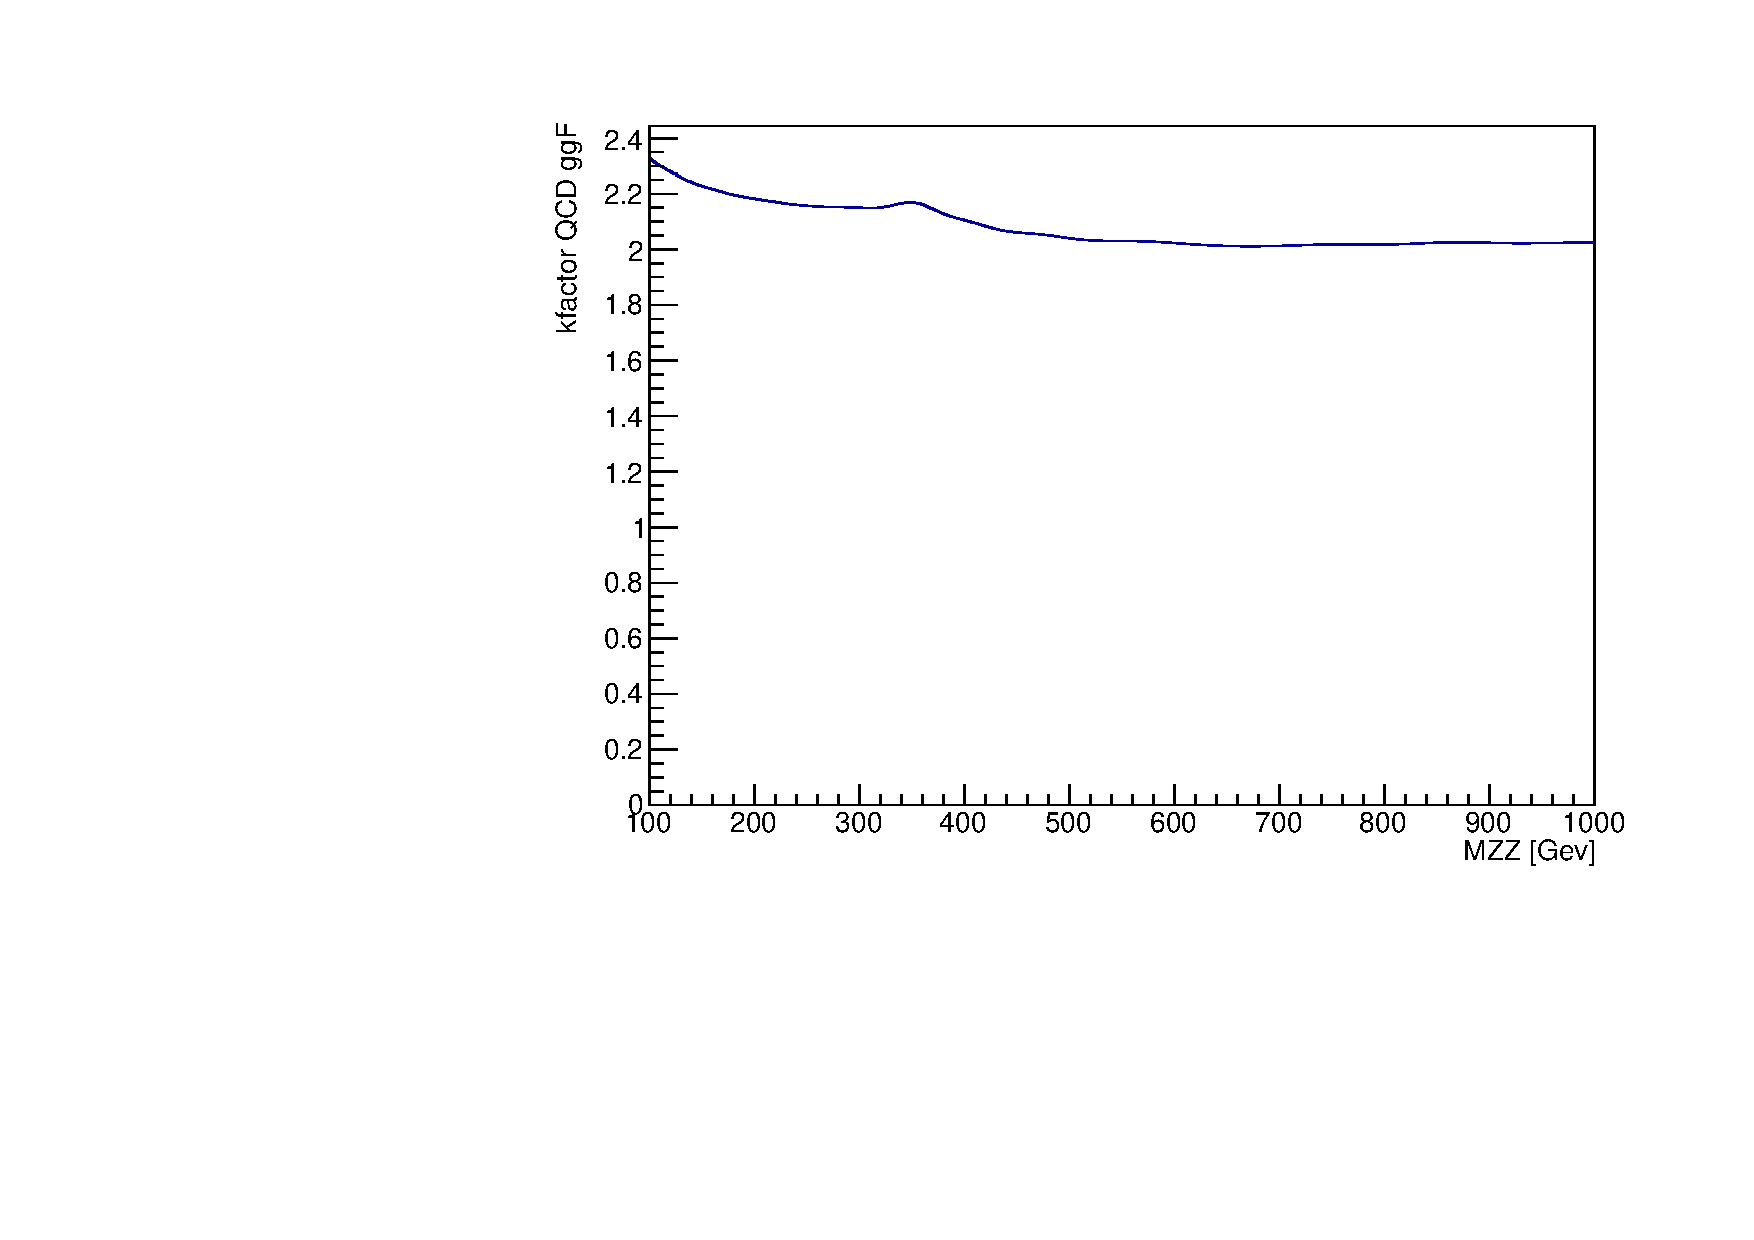
\includegraphics[width=0.7\textwidth]{kfqcd_ggF.pdf}
\caption {LO to NNLO $K$ factor as a function of ZZ invariant mass for ggH samples.}
\label{fig:kfggf}
\end{figure*}

The gluon fusion simulation is performed at LO and a mass dependent LO to NNLO $K$ factor is applied which is presented in Figure~\ref{fig:kfggf}. 
All \offshell production simulations are conducted at LO in QCD, with higher-order corrections 
included through a $K$ factor. In the gluon fusion process, the factorization and renormalization scales are set to run dynamically by equating them to $m_{4\ell}/2$. To incorporate higher-order QCD corrections, signal cross section calculations are performed at leading order (LO), next-to-leading order (NLO), and next-to-next-to-leading order (NNLO) using the MCFM and HNNLO 2 programs~\cite{Catani:2007vq,Grazzini:2008tf,Grazzini:2013mca} under the narrow-width approximation, covering a broad range of masses spanning both the on-shell and off-shell regions.

The ratios of NNLO to LO cross sections, referred to as NNLO-to-LO $K$ factors, are used to reweight~\cite{deFlorian:2016spz} the $m_{4\ell}$ distributions obtained from LO QCD simulations produced with MCFM and JHUGen. A constant $K$ factor 
% of 1.10 
is applied across the entire $m_{4\ell}$ spectrum to normalize the Higgs boson production cross section via gluon fusion to the next-to-next-to-next-to-leading order (N$^3$LO) prediction at $m_{4\ell} \approx 125$\,GeV~\cite{deFlorian:2016spz}. The $m_{4\ell}$ distributions from the POWHEG+JHUGen simulation of the $gg \to H$ process are reweighted using NNLO-to-NLO $K$ factors.

While the NNLO-to-LO $K$ factor is directly applicable to the signal, it serves only as an approximation for the $gg \to 4\ell$ background and its interference with the signal. An approximate NLO calculation~\cite{Caola:2015psa,Melnikov:2015laa,Campbell:2016ivq,Caola:2016trd} is available for both the background and the interference. The resulting NLO-to-LO $K$ factors for these components agree with the signal $K$ factor within approximately 10\% in the $m_{4\ell} > 220$\,GeV range relevant to this analysis. Consequently, the same NNLO-to-LO $K$ factor and N$^3$LO normalization, computed for the signal, are applied to the background and interference, along with their associated uncertainties. An additional 10\% uncertainty is assigned to the background component, and a 5\% uncertainty—corresponding to the square root of the variation—is applied to the interference.


\subsubsection{EW processes}

% Using JHUGen+MCFM programs, we simulate the EW (VBF and VH) \Hboson production inclusively and the decay of the \Hboson 
% to all lepton flavors (including taus). The allowed vector boson decays are restricted to the hadronic modes in the VH process,
% because the EW simulation covers the $4\ell+2$jets final state.  
% Furthermore, these LO samples are generated with lepton and jet cuts. The lepton cuts are the same as applied on the
% gluon fusion sample discussed above and do not affect final selection after reconstruction. 
% The jet cuts reduce the number of selected events by about $15\%$, affecting only the non-VBF and non-VH topology. 
% The YR4~\cite{YellowRep4} calculation includes cross sections of the individual EW processes 
% (VBF, ZH, WH) up to NNLO QCD and NLO EW for the \onshell region. As in the case of the gluon fusion processes, we compare the 
% \onshell cross section of the simulated EW processes to the cross-section reported in YR4 and extract a universal correction 
% (k factor) to be applied in all EW simulated processes (pure signal, interference, and background). To perform the comparison, 
% the GEN cut efficiency is applied to each of the EW YR4 numbers, the V to hadronic branching fraction (taken from Reference~\cite{Zyla:2020zbs}) 
% is applied to WH and ZH cross sections and finally the $H\to4\ell$ including $\tau$ branching fraction is applied to all numbers. 
% The three results are summed and compared to the simulated pure signal sample cross-section, estimated at the \Hboson mass peak. 
% The procedure is summarized in Table~\ref{tab:ew_YR4}. We utilize the YR4 uncertainties for the NNLO cross section, and estimate 
% an inclusive uncertainty per source on the $K$ factor. The estimated LO to NNLO QCD and NLO EW $K$ factor is estimated to be 
% \textbf{1.039} $\{{}^{+1.33\%}_{-0.8\%}(\mathrm{QCD\,scale})\pm 1.89\%(\mathrm{PDF})\pm 0.65\%(\alpha_\mathrm{strong})\}$.

Using the JHUGen+MCFM programs, we simulate EW Higgs boson production via VBF and VH processes, with inclusive decays of the Higgs boson to all lepton flavors (including $\tau$ leptons). In the VH process, the vector boson decays are restricted to hadronic modes, as the EW simulation is designed to model the $4\ell + 2$\,jets final state.

These LO samples are generated with generator-level lepton and jet cuts. The lepton cuts are identical to those applied in the gluon fusion simulation described earlier and do not affect the final event selection after reconstruction. The jet cuts, however, reduce the number of selected events by approximately 15\%, impacting only topologies that are not explicitly VBF- or VH-tagged.

YR4 provides cross-section predictions for individual EW processes (VBF, ZH, WH) in the \onshell region, calculated up to NNLO in QCD and NLO in EW corrections~\cite{YellowRep4}. As in the gluon fusion case, we compare the \onshell cross section of the simulated EW samples to the YR4 predictions and extract a universal correction factor ($K$ factor) to be applied consistently across all EW simulated samples, including pure signal, interference, and background contributions.

For this comparison, we apply the generator-level (GEN) selection efficiency to each YR4 cross-section value. Additionally, for WH and ZH processes, we multiply by the hadronic branching fraction of the vector boson (taken from Reference~\cite{Zyla:2020zbs}). Finally, the $H \to 4\ell$ branching fraction (including decays to $\tau$ leptons) is applied to all processes. The resulting three contributions are summed and compared to the simulated pure signal cross section at the Higgs boson mass peak. This procedure is summarized in Table~\ref{tab:ew_YR4}.

We adopt the uncertainties reported in YR4 for the NNLO cross section and estimate an inclusive uncertainty for each source contributing to the $K$ factor. The resulting LO-to-NNLO QCD and NLO EW correction factor is:
\[
K = \mathbf{1.039} \quad \left\{{}^{+1.33\%}_{-0.8\%} \,(\text{QCD scale}) \,\pm\, 1.89\% \,(\text{PDF}) \,\pm\, 0.65\%\, (\alpha_\text{strong}) \right\}.
\]

\begin{table}[!hbt]
\begin{center}
\small
\begin{tabular}{lllllr}
\vspace{-0.2cm} \\
\hline
    & YR4 [pb]    & GEN cut efficiency  & V hadronic & $H\to4\ell$ & $\sigma $[pb]   \\
\hline
VBF & 3.782    & 62.073\% &    & 0.0002745 &  0.000644  \\
WH  & 1.373    & 52.611\% & 67.41\%  & 0.0002745 &  0.000134 \\
ZH  & 0.8839   & 55.867\% & 69.911\%   & 0.0002745 &  0.000095  \\
Total  &          &          &           &           &  0.000873  \\
\vspace{-0.2cm} \\
MC   &          &          &           &           &  0.000840 \\
\vspace{-0.2cm} \\
\hline
\vspace{-0.2cm} \\
\multicolumn{5}{l}{LO QCD+EW to NNLO QCD and NLO EW $K$ factor} &  \textbf{1.039} \\
\vspace{-0.2cm} \\
\hline
\end{tabular}
\caption{The calculation for the NLO to NNLO $K$ factor for the EW \offshell samples at the \Hboson mass peak (125 GeV). 
The calculated factor is applied to all the \offshell EW MC samples.
\label{tab:ew_YR4}}
\end{center}
\end{table}


The $q\bar{q} \to 4\ell$ background is simulated at NLO in QCD and LO in electroweak (EW) theory using POWHEG. The fully differential cross section for this process has been computed at NNLO in QCD~\cite{Grazzini:2015hta}, and a differential NNLO-to-NLO $K$ factor as a function of $m_{4\ell}$ is applied to the POWHEG sample. This $K$ factor is approximately 1.1 at $m_{4\ell} = 125$\,GeV and varies between 1.0 and 1.2 in the region $m_{4\ell} < 500$\,GeV. The uncertainty from missing EW corrections in the low-mass region ($m_{4\ell} < 2m_{Z}$) is small compared to QCD-related uncertainties.

To account for EW corrections, an NLO-to-LO $K$ factor~\cite{Bierweiler:2013dja} is applied to events containing two on-shell Z bosons. This $K$ factor decreases with increasing $m_{4\ell}$, from approximately 1.0 near 125\,GeV to around 0.9 in the high-mass region ($m_{4\ell} > 500$\,GeV). The associated uncertainty is the dominant systematic for the off-shell width measurement and is included as a function of $m_{4\ell}$.

% In the on-shell region, the EW background from $VVV$, $t\bar{t}VV$, and $t\bar{t}V$ processes is generated using MadGraph5\_aMC@NLO~\cite{Alwall:2014hca}.

\section{Matrix Element Likelihood Approach} \label{sec:mela}

With up to 13 observables ($\boldsymbol{\Omega}$) describing the \Hboson kinematic distributions in the $2\to 6$ process, as visualized in Figure~\ref{fig:MELA}, it can be a challenging task to perform an optimal analysis. %in a multidimensional space of observables. 
MELA lets us calculate the matrix elements (ME) for each Higgs boson interaction as a function of its couplings and interacting particles. We can utilize these ME in ratios to change our hypotheses and reweight our Monte-Carlo samples, or treat them as probabilities and construct discriminants from the ME to use as observables (as discussed further in Section~\ref{sec:categories}). 

\begin{figure}[!hbt]
\centering
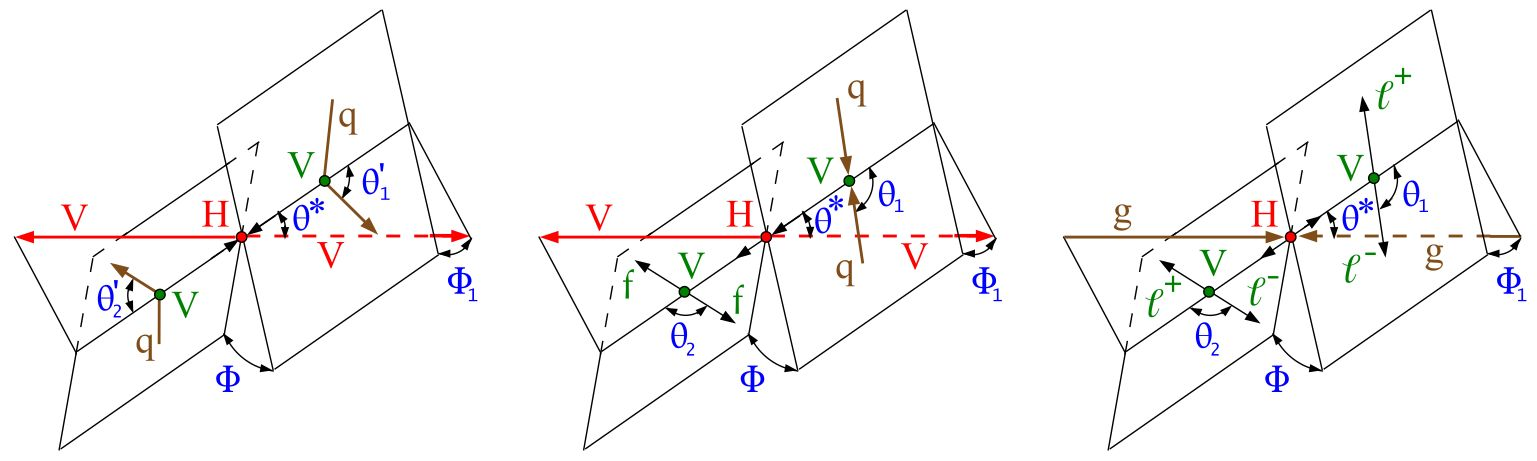
\includegraphics[width=0.8\textwidth,clip] {figures/MELA.jpg}
\caption{Diagrams of relevant kinematic observables in VBF (left), VH (center), and ggH (right) production modes of the Higgs boson.}
\label{fig:MELA}
\end{figure}

The MELA approach is designed to reduce the number of observables to the minimum while retaining all essential information. This is a very powerful tool which ensures that our analysis observables are still based in first principles, while affording us the flexibility to reweight distributions to new hypotheses or combine differently simulated statistics for greater precision in a single measurement. 

% In order to perform a dedicated study of the particular kinematic topology of HVV, visualized in \ref{fig:MELA}, events are split into several mutually 
% exclusive categories based on the presence of other particles produced in association with the \Hboson candidate~\cite{Sirunyan:2021rug}.
% We use the values of kinematic discriminants, and other selection requirements to perform the categorization. 

% \begin{figure}[!hbt]
% \centering
% 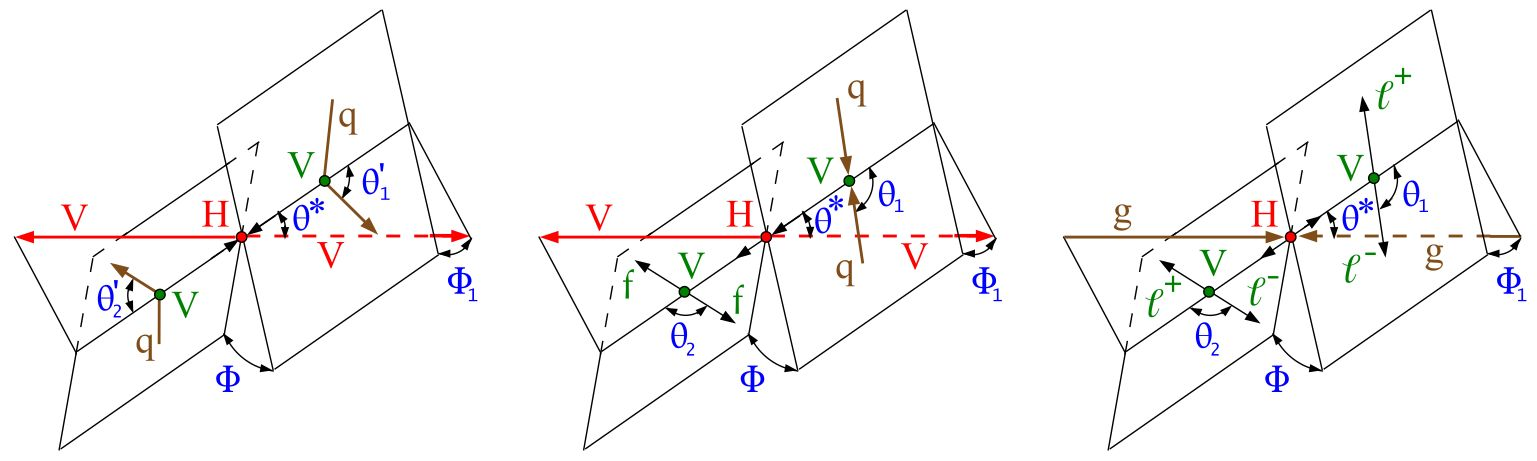
\includegraphics[width=0.8\textwidth,clip] {figures/MELA.jpg}
% \caption{Diagrams of relevant kinematic observables in VBF (left), VH (center), and ggH (right) productions of the Higgs boson.}
% \label{fig:MELA}
% \end{figure}

% The definition of these discriminants can be found in Refs.~\cite{Sirunyan:2017exp,Sirunyan:2017tqd,Sirunyan:2019twz,Sirunyan:2021rug}. 
% They are calculated using the MELA approach while employing the matrix elements at leading order (LO) in quantum chromodynamics (QCD). 

% \begin{equation}
% \mathcal{D}_\mathrm{alt}\left(\boldsymbol{\Omega}\right) = \frac{\mathcal{P}_\text{sig}\left(\boldsymbol{\Omega}\right) }
% {\mathcal{P}_\text{sig}\left(\boldsymbol{\Omega}\right) +\mathcal{P}_\mathrm{alt}\left(\boldsymbol{\Omega}\right) }
% \label{eq:melaD}
% \end{equation}

% \begin{equation}
% \mathcal{D}_\mathrm{int}\left(\boldsymbol{\Omega}\right) =
% \frac{\mathcal{P}_\mathrm{int}\left(\boldsymbol{\Omega}\right) }
% {2 \ \sqrt{{\mathcal{P}_\text{sig}\left(\boldsymbol{\Omega}\right) \ \mathcal{P}_\mathrm{alt}\left(\boldsymbol{\Omega}\right) }}}
% \label{eq:melaDint}
% \end{equation}

% These discriminants use full kinematic information from the \Hboson and from associated jet production and 
% are labeled to indicate a specific topology (2jet) and production mechanism (VBF, WH, ZH), 
% which is discriminated against the dominant gluon fusion process:
% %$\mathcal{D}_\mathrm{1jet}^{VBF}$, 
% $\mathcal{D}_\mathrm{2jet}^{VBF}$, 
% $\mathcal{D}_\mathrm{2jet}^{ZH}$,
% and $\mathcal{D}_\mathrm{2jet}^{WH}$. 
% %The $\mathcal{D}_\mathrm{2jet}$ discriminants are calculated using both SM and anomalous coupling hypotheses, 
% %leading to a set $\mathcal{D}_\mathrm{2jet}^{i}$, all of which 
% %are tested in order to maintain high efficiency of VBF and VH categorization in the presence of anomalous couplings. 
% % Calculation of these discriminants is discussed in more detail later with the presented analysis. 

% % The MELA approach also allows for reweighting between our simulated probability distributions. This has the effect of reducing the number of dedicated 
% % Monte-Carlo simulations required for this analysis, as well as bolstering the available statistics that can be utilized in our templates for Bayesian analysis. 

% \begin{figure}
% \centering
% 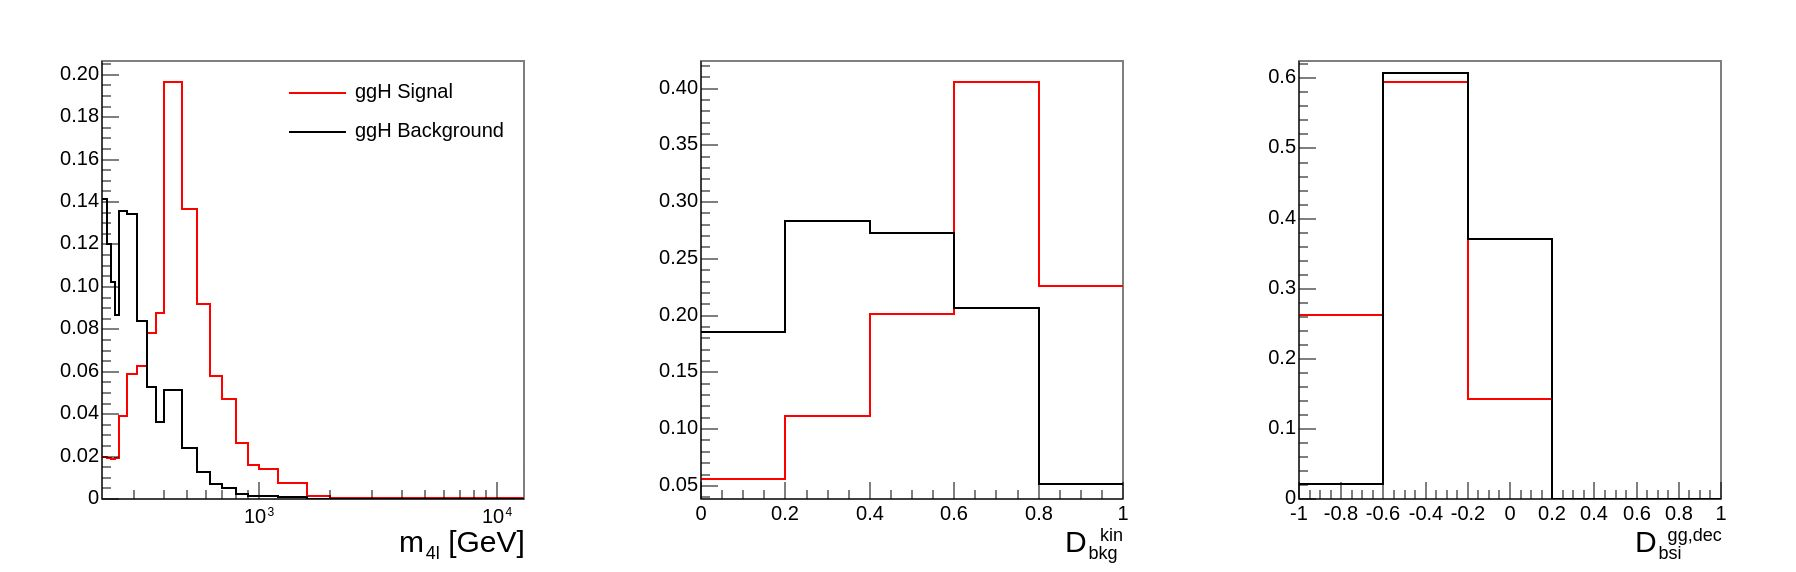
\includegraphics[width=0.8\textwidth,clip] {figures/DiscDists.jpg}
% \caption{}
% \label{fig:DiscDists}
% \end{figure}

\section{Building a $H^{(*)} \to ZZ^{(*)} \to 4\ell$ analysis}

\subsection{Reconstructing and selecting events} \label{sec:recoandsel}

% Event reconstruction is based on the particle-flow (PF) algorithm~\cite{Sirunyan:2017ulk}. This algorithm aims to reconstruct and identify each individual particle in an event, with an optimized combination of information from the various elements of the CMS detector. The energy of photons is obtained from the ECAL measurement. The energy of electrons is determined from a combination of the electron momentum at the primary vertex as determined by the tracker, the energy of the corresponding ECAL cluster, and the energy sum of all bremsstrahlung photons spatially compatible with originating from the electron track. The energy of muons is obtained from the curvature of the corresponding track. The energy of charged hadrons is determined from a combination of their momentum measured in the tracker and the matching ECAL and HCAL energy deposits, corrected for the response function of the calorimeters to hadronic showers. Finally, the energy of neutral hadrons is obtained from the corresponding corrected ECAL and HCAL energies.

% Muons with $p_T > 5$ GeV are reconstructed within the geometrical acceptance, corresponding to the region $|\eta|< 2.4$, by combining information from the silicon tracker and the muon systems \cite{MuReco}. The muons are selected among the reconstructed muon track candidates by applying quality requirements on the track in both the muon and silicon tracker systems, and demanding small energy deposits in the calorimeters.

Event reconstruction is based on the particle-flow (PF) algorithm~\cite{Sirunyan:2017ulk}, which endeavors to reconstruct and identify each individual particle in an event by combining information from the various subdetectors of the CMS experiment. PF candidates are classified as photons, electrons, or muons, and they are then used to build higher-level objects, such as jets. 

Photon energies are determined directly from ECAL measurements, and are not expected to present a signal in the HCAL or tracker. Electrons are identified from a multivariate discriminant involving their momentum at the PV as measured by the tracker, a geometrically corresponding ECAL cluster of energy deposition, and the integrated energy of all bremsstrahlung (radiated) photons determined to be spatially consistent with emission from the electron's trajectory~\cite{Sirunyan:2021rug}. Muons, like electrons, also start in the tracker, but have trajectories and momenta that can be extrapolated to the muon system while depositing little to no energy in the ECAL and HCAL. Their energies are inferred from the curvature of their tracks in the magnetic field. After the isolated muons, electrons, and photons are classified, the remaining particles are used to identify hadrons. For charged hadrons, energies are determined by combining their momenta measured in the tracker with the corresponding ECAL and HCAL energy deposits. The energies of neutral hadrons are obtained from their corrected ECAL and HCAL energy deposits.

Electrons are reconstructed within the geometrical acceptance defined by $|\eta| < 2.5$ and transverse momentum $p_{\mathrm{T}} > 7$\,GeV~\cite{eleReco}. While muons with transverse momentum $p_T > 5$ GeV are reconstructed within the geometrical acceptance of $|\eta|< 2.4$. Candidates are reconstructed using information from both the silicon tracker and the muon detection systems~\cite{MuReco}. Then, the selection of muons from among the reconstructed muon track candidates is subject to stringent quality criteria applied to tracks in both the muon chambers and the silicon tracker, complemented by requirements of minimal energy deposition in the calorimeter systems, ensuring high purity in the muon identification.

Additionally, to distinguish prompt lepton products of high-$p_T$ $Z$ boson decays from those originating in hadronic jets---such as leptons produced in electroweak decays of hadrons---an isolation requirement is applied. For muons, an isolation variable is computed to quantify the level of surrounding activity and suppress backgrounds from non-prompt sources~\cite{Sirunyan:2021rug}. The isolation variable is defined relative to the muon's transverse momentum $p_T$ as
\begin{equation} \label{eqn:pfiso}
  {\mathcal I}^{\mu} \equiv \Big( \sum p_T^\text{charged} + \max\big[ 0, \sum p_T^\text{neutral} +
    \sum p_T^{\gamma} - p_T^{\mathrm{PU}} \big] \Big) / p_T,
\end{equation}
where $p_T^{\text{charged}}$, $p_T^\text{neutral}$, and $p_T^\gamma$ are summed over the charged and neutral hadrons and photons within a cone radius of $\Delta R \equiv \sqrt{\smash[b]{(\eta^i-\eta^j)^{2} + (\phi^i-\phi^j)^{2}}} = 0.3$ around the lepton's direction at the interaction vertex. Here, $\phi$ denotes the azimuthal angle and indices $\textit{i}$ and $\textit{j}$ refer to the hadron or photon and muon, respectively. This isolation variable exhibits particular sensitivity to energy deposits from pileup interactions. Therefore, a contribution $p_T^{\mathrm{PU}}$ from pileup is subtracted, as seen in Equation~(\ref{eqn:pfiso})~\cite{PUmitigationCMS}. Finally, each muon in a selected event must satisfy ${\mathcal{I}^{\mu}} < 0.35$.
% This term is defined as $p_T^{\mathrm{PU}} = 0.5\sum_{i}p_T^{i,\mathrm{PU}}$, involving the sum of $p_T$ over all charged hadrons $i$ not originating from the PV, where the factor of 0.5 accounts for the differing fractions of charged and neutral hadrons~\cite{PUmitigationCMS}. 

Instead of applying a separate isolation requirement---as in the case for muons---the electron multivariate discriminant incorporates the isolation sums ($\sum p_{\mathrm{T}}^{\text{charged}}$, $\sum p_{\mathrm{T}}^{\text{neutral}}$, and $\sum p_{\mathrm{T}}^{\gamma}$) directly~\cite{Sirunyan:2021rug}. The inclusion of these isolation components offers better performance for electrons compared to a simple threshold on the relative isolation variable. The XGBOOST (eXtreme Gradient Boosting) library is used on simulated events to train and optimize the multivariate discriminant employed for electron identification and isolation. Events are separated into six regions, defined by two transverse momentum ranges ($7 < p_{\mathrm{T}} < 10$\,GeV and $p_{\mathrm{T}} > 10$\,GeV) and three pseudorapidity intervals: the central barrel ($|\eta_{e}| < 0.8$), outer barrel ($0.8 < |\eta_{e}| < 1.479$), and endcaps ($1.479 < |\eta_{e}| < 2.5$). Separate discriminant training is performed for each of the three data-taking periods in Run 2, and the selection requirements are optimized such that the signal efficiency is uniform across all three periods.

The effect of the final-state radiation (FSR) from leptons are also recovered~\cite{Sirunyan:2017ulk}. (Bremsstrahlung photons already associated to electrons in the reconstruction step are not considered.) Isolated photons satisfying $p_T^\gamma>2$ GeV, $|\eta^\gamma| <2.4$, and $\mathcal{I}^{\gamma} < 1.8$ are associated with the nearest selected lepton (muon or electron) in the event. Photons must also satisfy the criteria $\Delta R(\gamma,\ell)/(p_T^{\gamma})^2<0.012~\text{GeV}^{-2}$ and $\Delta R(\gamma,\ell) < 0.5$. When multiple photon candidates fulfill these conditions, the one minimizing $\Delta R(\gamma,\ell)/(p_T^{\gamma})^2$ with respect to the given lepton is retained. FSR photons are excluded from the computation of the relative isolation parameter.

% Electrons with $p_T>7$ GeV are reconstructed within the geometrical acceptance, defined by the pseudorapidity region $|\eta|<2.5$~\cite{eleReco}. Their identification utilizes a multivariate discriminant incorporating observables sensitive to bremsstrahlung emission along the electron trajectory, the geometric and momentum-energy matching between the electron trajectory and associated ECAL cluster, the electromagnetic shower morphology in the ECAL, and variables discriminating against electrons originating from photon conversions. Electron isolation parameters, defined analogously to those for muons, are integrated into this multivariate discriminant to differentiate between prompt leptons from Z boson decays and those arising from electroweak decays of hadrons within jets. The XGBoost package~\cite{xgboost} is employed for training and optimization of this multivariate discriminant using simulated events that remain independent from all other analysis stages. Separate training procedures are implemented for each of the three data-taking periods \cite{ElectronBDT}. Electrons from photon conversions and muons from in-flight hadronic decays are rejected if the ratio of their three-dimensional impact parameter, computed with respect to the primary vertex position, to its uncertainty exceeds four.



A ``tag-and-probe'' technique~\cite{CMS:2011aa}, based on samples of $Z$ boson events in both data and simulation, is employed to measure the reconstruction and selection efficiencies for prompt electrons and muons across bins of transverse momentum ($p_{\mathrm{T}}$) and pseudorapidity ($\eta$). The differences between the efficiencies measured in data and those obtained from simulation are used to derive correction factors, which are applied to rescale the event yields in the simulated samples~\cite{Sirunyan:2021rug}. These simulated events are also utilized to calibrate the momentum scale and resolution of prompt leptons, again in bins of $p_{\mathrm{T}}$ and $\eta$~\cite{ScaleSmear2, Roch2}.


% The reconstruction and selection efficiencies for prompt leptons in both data and simulation are evaluated using a tag-and-probe technique~\cite{CMS:2011aa} applied to $Z$ boson event samples. The ratio of efficiencies measured in data to those in simulation is applied as a correction factor to the yields of selected events in the simulated samples.


For this analysis, selection of Higgs boson candidates requires four prompt and isolated leptons following the aforementioned criteria. One lepton must satisfy $p_T>20$ GeV and at least one additional lepton must have $p_T>10$ GeV. Then, Z boson candidates are constructed from $e^+e^-$ or $\mu^+\mu^-$ pairs with invariant masses in the range 12--120 GeV. These dilepton pairs are combined to form a Higgs boson candidate. 
We choose $Z_1$ to label the pair with invariant mass closest to the nominal Z boson mass, 
and call the remaining pair $Z_2$. 

Four possible combinations are considered and treated independently: 
$4\mu$, $4e$, $2e2\mu$, and $2\mu2e$, where the mixed-flavor final states are distinguished based on the flavor composition of $Z_{1}$. These four combinations exhibit different four-lepton mass resolutions (predominantly determined by the flavor composition of $Z_{1}$) and contain different amounts of reducible background (largely dependent on the flavor composition of $Z_{2}$). Since none of these flavor-dependent characteristics impact the off-shell \Hboson analysis, all flavor channels are combined to make our measurement~\cite{PhysRevD.111.092014}. 

Signal candidates must satisfy $m_{4\ell} > 70$ GeV. When multiple \Hboson candidates can be formed in an event, the one with the highest value of the kinematic discriminant $\mathcal{D}_\text{bkg}^\text{kin}$ (defined in Section~\ref{sec:categories}) is chosen, However, if these \Hboson candidates are comprised of the same four leptons, the candidate whose $Z_1$ invariant mass lies closest to the nominal Z boson mass is selected.

In this off-shell analysis, events undergo further categorization based on jets associated with the \Hboson candidate~\cite{PhysRevD.111.092014}. Jets are clustered using the anti-$k_t$ jet finding algorithm~\cite{Cacciari:2008gp,Cacciari:2011ma} with a distance parameter of 0.4. The jet momentum is determined as the vector sum of all constituent particle momenta. 
Jets must satisfy $p_T>30$ GeV and $|\eta|<4.7$ and must be spatially separated
from all selected lepton candidates and any selected FSR photons by requiring 
$\Delta R(\ell/\gamma,\text{jet})>0.4$.
Jets originating from b quark hadronization are identified using the DeepCSV algorithm~\cite{Sirunyan:2017ezt}, which integrates information 
on impact parameter significance, secondary vertex characteristics, and jet kinematic variables. These b-tagged jets are then used as part of our criteria for categorizing events, as detailed in Section~\ref{sec:categories}.

% Here, $\Delta R(i,j) Equation \refuiv \sqrt{\smash[b]{(\eta^i-\eta^j)^{2} + (Hi^i-Hi^j)^{2}}}$, where $Hi$ is the azimuthal angle, and in this case $\textit{i}$ refers to the hadron or photon, and $\textit{j}$ to the muon.
% Since the isolation variable is particularly sensitive to energy deposits from pileup interactions, a contribution $p_T^{\mathrm{PU}}$ from pileup is subtracted from the isolation parameter, as shown in Equation~(\ref{eqn:pfiso}). 
% It is defined as 0.5 times the $p_T$ sum of all charged hadrons $i$ not originating from the primary vertex $p_T^{\mathrm{PU}} = 0.5\sum_{i}p_T^{i,\mathrm{PU}}$, where the 0.5 factor accounts for the different fraction of charged and neutral hadrons~\cite{PUmitigationCMS}. A requirement of ${\mathcal{I}^{gm}} < 0.35$ is placed on each muon in the event.

% Photons from final-state radiation are reconstructed using the PF algorithm~\cite{Sirunyan:2017ulk}. Isolated photons with $p_T >2$ GeV, $|\eta| <2.4$, and $\mathcal{I}^{\gamma} < 1.8$, are associated with the closest lepton (either muon or electron) in the event. Photons that do not satisfy the requirements $\Delta R(gg,\ell)/(p_T^{\gamma})^2<0.012 GeV^{-2}$ and $\Delta R(gg,\ell) < 0.5$ are discarded.
% If more than one photon candidate fulfils the above conditions, the one with the lowest value of $\Delta R(gg,\ell)/(p_T^{\gamma})^2$ with respect to the given lepton is retained.
% Photons passing the above criteria are excluded from the computation of the relative isolation parameter. 

% Electrons with $p_T>7$ GeV are reconstructed within the geometrical acceptance, corresponding to the pseudorapidity region $|\eta|<2.5$~\cite{eleReco}. They are identified using a multivariate discriminant, which includes observables sensitive to the emission of bremsstrahlung along the electron trajectory, the geometrical and momentum-energy matching between the electron trajectory and the associated cluster in the ECAL, the shape of the electromagnetic shower in the ECAL, and variables that discriminate against electrons originating from photon conversions. The isolation parameter sums for electrons, defined similarly as for muons, are included in the multivariate discriminant. This information is used to discriminate between prompt leptons from Z boson decays and those arising from EW decays of hadrons within jets. The package XGBoost~\cite{xgboost} is used to train and optimize this multivariate discriminant. The training is performed with simulated events that are not used at any other stage of the analysis. Separate trainings are performed for the three different data-taking periods \cite{ElectronBDT}. Electrons from photon conversions and muons from in-flight decays of hadrons are rejected if the ratio of their impact parameter in three dimensions, computed with respect to the primary vertex position, to their uncertainty is greater than four.

% The reconstruction and selection efficiencies for prompt leptons in both data and simulation have been estimated using a tag-and-probe technique~\cite{CMS:2011aa} based on samples of $Z$ boson events. The ratio of the efficiencies measured in data and simulation is used to rescale the yields of selected events in the simulated samples.
% In addition, $Z$ boson events have been used to calibrate the momentum scale and resolution of electrons and muons in bins of different kinematic variables~\cite{ScaleSmear2, Roch2}.

% In the selection of Higgs boson candidates,
% four prompt and isolated leptons are required following the prescription above. 
% One of the leptons must have $p_T>20$ GeV and at least one of the remaining leptons must satisfy $p_T>10$ GeV.
% The Z boson candidates are constructed from $epem$ or $gmpgmm$ pairs whose  invariant mass is in the range 12--120 GeV. 
% The dilepton pairs are then combined to form the Higgs boson candidate. 
% In the following, $Z_1$ denotes the pair with the mass closest to the nominal $Z$ boson mass, 
% while $Z_2$ refers to the remaining one. Four possible combinations are considered and treated separately: 
% 4gm, 4$e$, $2e2gm$, and $2gm2e$, where the mixed-flavor final states are separated based on the decay of $Z_{1}$. 
% The four possible combinations have different four-lepton mass resolutions (largely driven by whether the $Z_{1}$ is formed from 2$gm$ or 2$e$) 
% and different amounts of reducible background (largely driven by whether the $Z_{2}$ decays to 2$\mu$ or 2$e$).
% None of the above differences between the flavor channels affect the off-shell \Hboson analysis 
% and therefore all flavor channels are combined in that measurement. 
% Signal candidates must satisfy $m_{4\ell} > 70$ GeV. 
% If more than one \Hboson candidate can be formed in the event, the one with the highest value of the 
% kinematic discriminant $\mathcal{D}_\text{bkg}^\text{kin}$, defined in Section~\ref{sec:Discriminants},
% is retained, unless these candidates consist of the same four leptons. 
% In this case, the candidate with the $Z_1$ invariant mass closest to the nominal Z boson mass is retained.

% In the off-shell analysis, events are further categorized based on the jets associated with the \Hboson candidate. 
% The jets are clustered using the anti-\kt jet finding algorithm~\cite{Cacciari:2008gp,Cacciari:2011ma} with a distance 
% parameter of 0.4. The jet momentum is determined as the vector sum of all particle momenta in the jet. 
% Jets must satisfy $p_T>30$ GeV and $|\eta|<4.7$ and must be separated
% from all selected lepton candidates and any selected final-state radiation photons by demanding 
% $\Delta R(\ell/\cPgg,{\text{jet}})>0.4$.
% Jets originating from the hadronization of b quarks are identified using the DeepCSV algorithm~\cite{Sirunyan:2017ezt}, which combines information 
% on impact parameter significance, the secondary vertex, and jet kinematic variables. The use of this identification is described in Section~\ref{sec:Discriminants}.

























\subsection{Defining categories and observables} \label{sec:categories}

% With up to 13 observables, $\boldsymbol{\Omega}$, describing the \Hboson kinematic distributions in the $2\to 6$ process,
% it is a challenging task to perform an optimal analysis in a multidimensional space of observables. 
% The MELA approach is designed to reduce the number of observables to the minimum while retaining all essential information. 
% Two types of discriminants were defined for either the production or decay process, and we also combine them into a joint 
% discriminant for the full $2\to 6$ process where relevant.

% \begin{figure}[!hbt]
% \centering
% 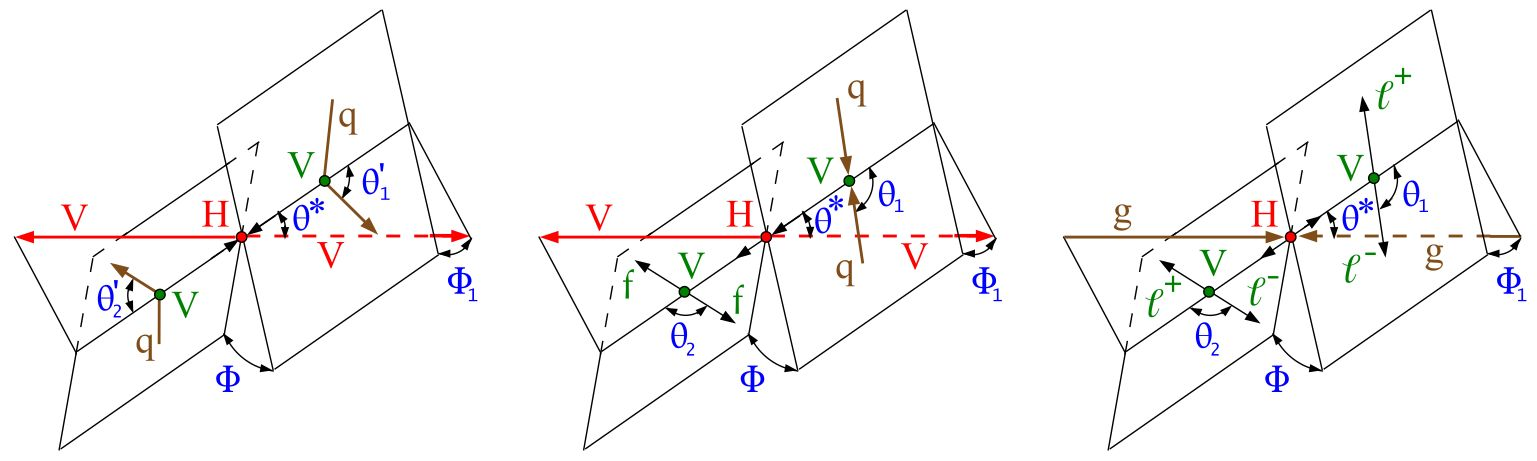
\includegraphics[width=0.8\textwidth,clip] {figures/MELA.jpg}
% \caption{Diagrams of relevant kinematic observables in VBF (left), VH (center), and ggH (right) productions of the Higgs boson.}
% \label{fig:MELA}
% \end{figure}

In order to perform a dedicated study of the particular kinematic topology of HVV, visualized in Figure~\ref{fig:MELA}, events are split into several mutually exclusive categories based on the presence of other particles produced in association with the \Hboson candidate~\cite{Sirunyan:2021rug}. Two types of discriminants are defined for either the production or decay process, which can be combined to describe the full $2\to 6$ process~\cite{Sirunyan:2017exp,Sirunyan:2017tqd,Sirunyan:2019twz,Sirunyan:2021rug}. We use the values of these kinematic discriminants and other selection requirements to perform the categorization. They are calculated using the MELA approach while employing the matrix elements at leading order (LO) in quantum chromodynamics (QCD):
\begin{equation}
	\mathcal{D}_\mathrm{alt}\left(\boldsymbol{\Omega}\right) = \frac{\mathcal{P}_\text{sig}\left(\boldsymbol{\Omega}\right) }
	{\mathcal{P}_\text{sig}\left(\boldsymbol{\Omega}\right) +\mathcal{P}_\mathrm{alt}\left(\boldsymbol{\Omega}\right) }
	\label{eq:melaD}
\end{equation}
\begin{equation}
	\mathcal{D}_\mathrm{int}\left(\boldsymbol{\Omega}\right) =
	\frac{\mathcal{P}_\mathrm{int}\left(\boldsymbol{\Omega}\right) }
	{2 \ \sqrt{{\mathcal{P}_\text{sig}\left(\boldsymbol{\Omega}\right) \ \mathcal{P}_\mathrm{alt}\left(\boldsymbol{\Omega}\right) }}},
	\label{eq:melaDint}
\end{equation}

where the probability of a certain process $\mathcal{P}$ is calculated using the full kinematics characterized
by $\boldsymbol{\Omega}$ for the hypotheses denoted as ``sig'' for a signal model and ``alt'' for an alternative model,
which could be an alternative \Hboson production mechanism (used to categorize events),
background (used to isolate signal), or an alternative \Hboson coupling model (used to measure coupling parameters).
The ``int'' label represents the interference between the two model contributions.
The probabilities $\mathcal{P}$ are calculated from the matrix elements provided by the MELA package and
are normalized to give the same integrated cross sections in the relevant phase space of each process.

% These discriminants use full kinematic information from the \Hboson with its associated jets and 
% are labeled to indicate a specific topology (2jet) and production mechanism (VBF, WH, ZH), 
% which is discriminated against the dominant gluon fusion process:
% %$\mathcal{D}_\mathrm{1jet}^{VBF}$, 
% $\mathcal{D}_\mathrm{2jet}^{VBF}$, 
% $\mathcal{D}_\mathrm{2jet}^{ZH}$,
% and $\mathcal{D}_\mathrm{2jet}^{WH}$. 

%The $\mathcal{D}_\mathrm{2jet}$ discriminants are calculated using both SM and anomalous coupling hypotheses, 
%leading to a set $\mathcal{D}_\mathrm{2jet}^{i}$, all of which 
%are tested in order to maintain high efficiency of VBF and VH categorization in the presence of anomalous couplings. 
% Calculation of these discriminants is discussed in more detail later with the presented analysis. 

% The MELA approach also allows for reweighting between our simulated probability distributions. This has the effect of reducing the number of dedicated 
% Monte-Carlo simulations required for this analysis, as well as bolstering the available statistics that can be utilized in our templates for Bayesian analysis. 
 
A set of discriminants $\mathcal{D}_\text{2jet}$ is constructed, following Equation \ref{eq:melaD},
where $\mathcal{P}_\text{sig}$ corresponds to the signal probability for the VBF ($WH$ or $ZH$)
production hypothesis in the VBF-tagged (VH-tagged) category, and $\mathcal{P}_\mathrm{alt}$
corresponds to that of \Hboson production in association with two jets via gluon fusion.
These discriminants use full kinematic information from the \Hboson with its associated jets and 
are labeled to indicate a specific topology (2jet) and production mechanism (VBF, WH, ZH), 
which is discriminated against the dominant gluon fusion process:
$\mathcal{D}_\mathrm{2jet}^{VBF}$, 
$\mathcal{D}_\mathrm{2jet}^{ZH}$,
and $\mathcal{D}_\mathrm{2jet}^{WH}$.
When more than two jets pass the selection criteria, the two jets with the highest $p_T$ are chosen 
for the matrix element calculations. Thus, the $\mathcal{D}_\text{2jet}$ discriminants separate the 
target production mode of each category from gluon fusion production,
in all cases using only the kinematics of the \Hboson and two associated jets~\cite{PhysRevD.111.092014}.

% Sequential selection criteria are used to define the categories:
% \begin{itemize}
%     \item[--]  The VBF-2jet category requires exactly four leptons. In addition, there must be 
%     either two or three jets of which at most one is identified as coming from the hadronization of a b quark, which we term a b-tagged jet~\cite{Sirunyan:2021rug}, 
%     or at least four jets and no b-tagged jets. 
%     Finally, $\mathcal{D}_\text{2jet}^{VBF} >0.5$ is required~\cite{Sirunyan:2021rug}. 
    
%     \item[--]  The VH-hadronic category requires exactly four leptons. In addition, there must be
%     either two or three jets, or at least four jets and no b-tagged jets. 
%     Finally, we demand $\max(\mathcal{D}_\text{2jet}^{WH},~\mathcal{D}_\text{2jet}^{ZH} )>0.5$~\cite{Sirunyan:2021rug}.
    
%     \item[--]  The Untagged category consists of the remaining events.
% \end{itemize}

Sequential selection criteria are used to define the event categories:
\begin{itemize}
    \item[--] The VBF-2jet category requires exactly four leptons. In addition, events must contain either two or three jets with at most one identified as originating from a b quark (b-tagged jet)~\cite{Sirunyan:2021rug}, or at least four jets with no b-tagged jets. Furthermore, events must satisfy $\mathcal{D}_\text{2jet}^{VBF} > 0.5$~\cite{Sirunyan:2021rug}.
    
    \item[--] The VH-hadronic category requires exactly four leptons. Additionally, events must have either two or three jets, or at least four jets with no b-tagged jets. Events are required to satisfy $\max(\mathcal{D}_\text{2jet}^{WH},~\mathcal{D}_\text{2jet}^{ZH}) > 0.5$~\cite{Sirunyan:2021rug}.
    
    \item[--] The Untagged category comprises all remaining events.
\end{itemize}

The selected events are split into the three categories summarized with their observables in Table~\ref{tab:categoriesoffshell}: VBF-tagged, VH-tagged, and Untagged. Distributions of these discriminants are shown in Figures~\ref{fig:SelectionDiscriminant_D2jetVBF}, \ref{fig:SelectionDiscriminant_D2jetZH}, and \ref{fig:SelectionDiscriminant_D2jetWH}. Because the EW off-shell SM signal samples are dominated by VBF production, the fraction of VH events is predictably small, as reflected in Figures~\ref{fig:SelectionDiscriminant_D2jetZH} and \ref{fig:SelectionDiscriminant_D2jetWH}.

\begin{table}[!hbtp]
	\begin{center}
		\begin{tabular}{lccc}
			\hline
			\vspace{-0.2cm}  & & & \\
			~~Category              & VBF-tagged & $VH$-tagged  & Untagged \\
			\vspace{-0.2cm}    & & & \\
			\hline
			%
			\vspace{-0.2cm}  & & & \\
			%
			~~Selection
			& ~~$ \mathcal{D}_{\rm 2jet}^{\rm VBF} >0.5$ 
			& ~~$ \mathcal{D}_{\rm 2jet}^{ZH}$ or $ \mathcal{D}_{\rm 2jet}^{WH}>0.5$
			& ~~Rest of events \\
			%
			&
			& ~~~~
			&   \\
			%
			\vspace{-0.2cm}  & & & \\
			%
			Observables
			&  $m_{4\ell}$, $\mathcal{D}^{{\rm VBF}+{\rm dec}}_{\rm bkg}$, $\mathcal{D}_{\rm bsi}^{{\rm VBF}+{\rm dec}}$
			&  $m_{4\ell}$, $\mathcal{D}^{VH+{\rm dec}}_{\rm bkg}$, $\mathcal{D}_{\rm bsi}^{VH+{\rm dec}}$
			&  $m_{4\ell}$, $\mathcal{D}^{\rm kin}_{\rm bkg}$, $\mathcal{D}_{\rm bsi}^{{\rm gg},{\rm dec}}$  \\
			& & & \\
			% 
			\hline
			%
		\end{tabular}
	\end{center}
    \caption{Summary of the three production categories in the off-shell $m_{4\ell}$ region. All discriminants are calculated with the JHUGen signal and MCFM background matrix elements. The VH interference discriminant in the VH-tagged category is the simple average of the ones corresponding to the ZH and WH processes~\cite{PhysRevD.111.092014}.}
    \label{tab:categoriesoffshell}
\end{table}

%%%%%%%%%%%%%%%%%%%%%%%%%%%%%%%%%%%%%%%%%
\begin{figure*}[!hbt]
\centering
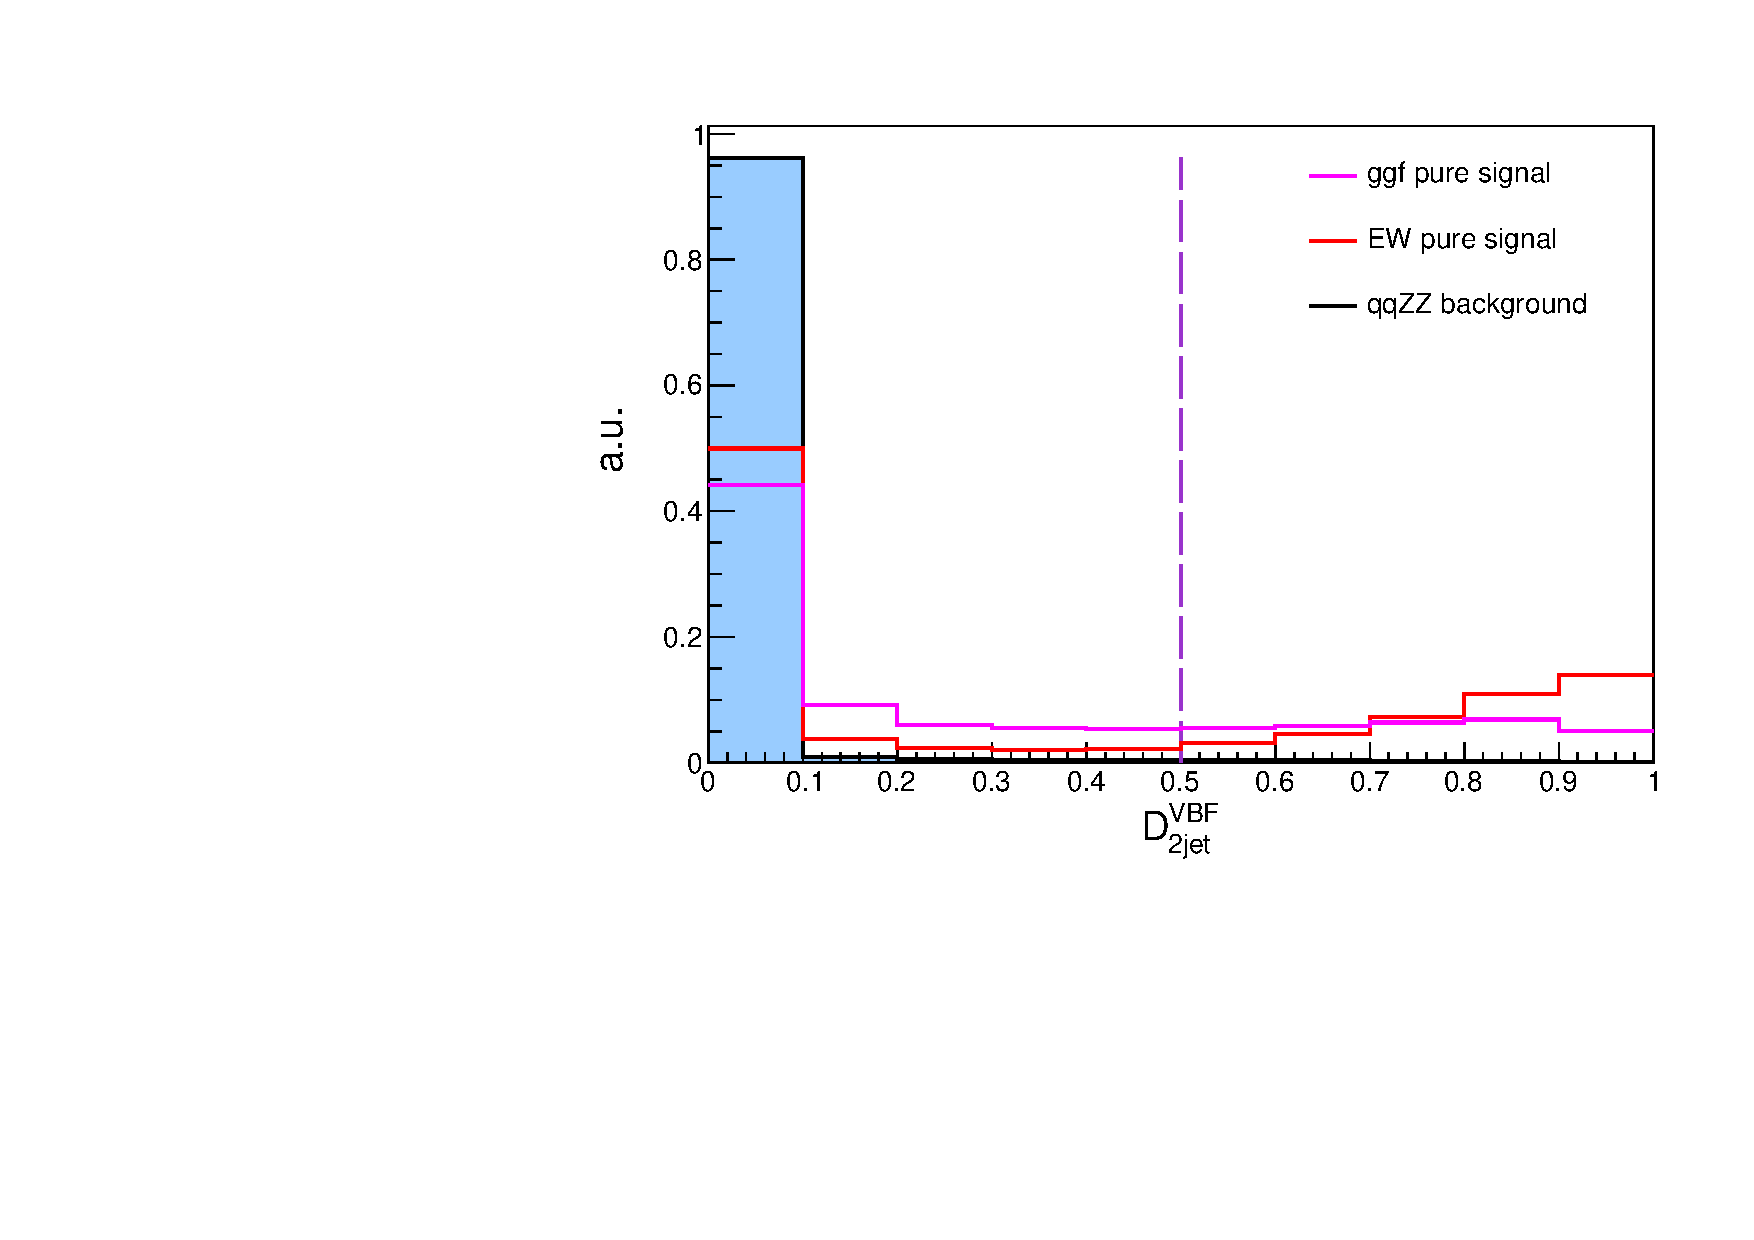
\includegraphics[width=0.8\textwidth]{figures/D2JVBF_cat.pdf}
\caption{
Distribution of the $\mathcal{D}_\mathrm{2jet}^{VBF}$ discriminant used in selection of the VBF-2jet category. 
Three distributions are shown in the \offshell selection region ($m_{4\ell}>220$ GeV):
SM signal \offshell production in gluon fusion (JHUGen+MCFM, magenta); 
SM signal \offshell EW production, including VBF, ZH, and WH (JHUGen+MCFM, red); 
$q\bar{q}\to 4\ell$ background production (shaded). 
The selection threshold of 0.5 is shown with the dashed line. 
}
\label{fig:SelectionDiscriminant_D2jetVBF}
\end{figure*}
%%%%%%%%%%%%%%%%%%%%%%%%%%%%%%%%%%%%%%%%%
%%%%%%%%%%%%%%%%%%%%%%%%%%%%%%%%%%%%%%%%%
\begin{figure*}[!hbt]
\centering
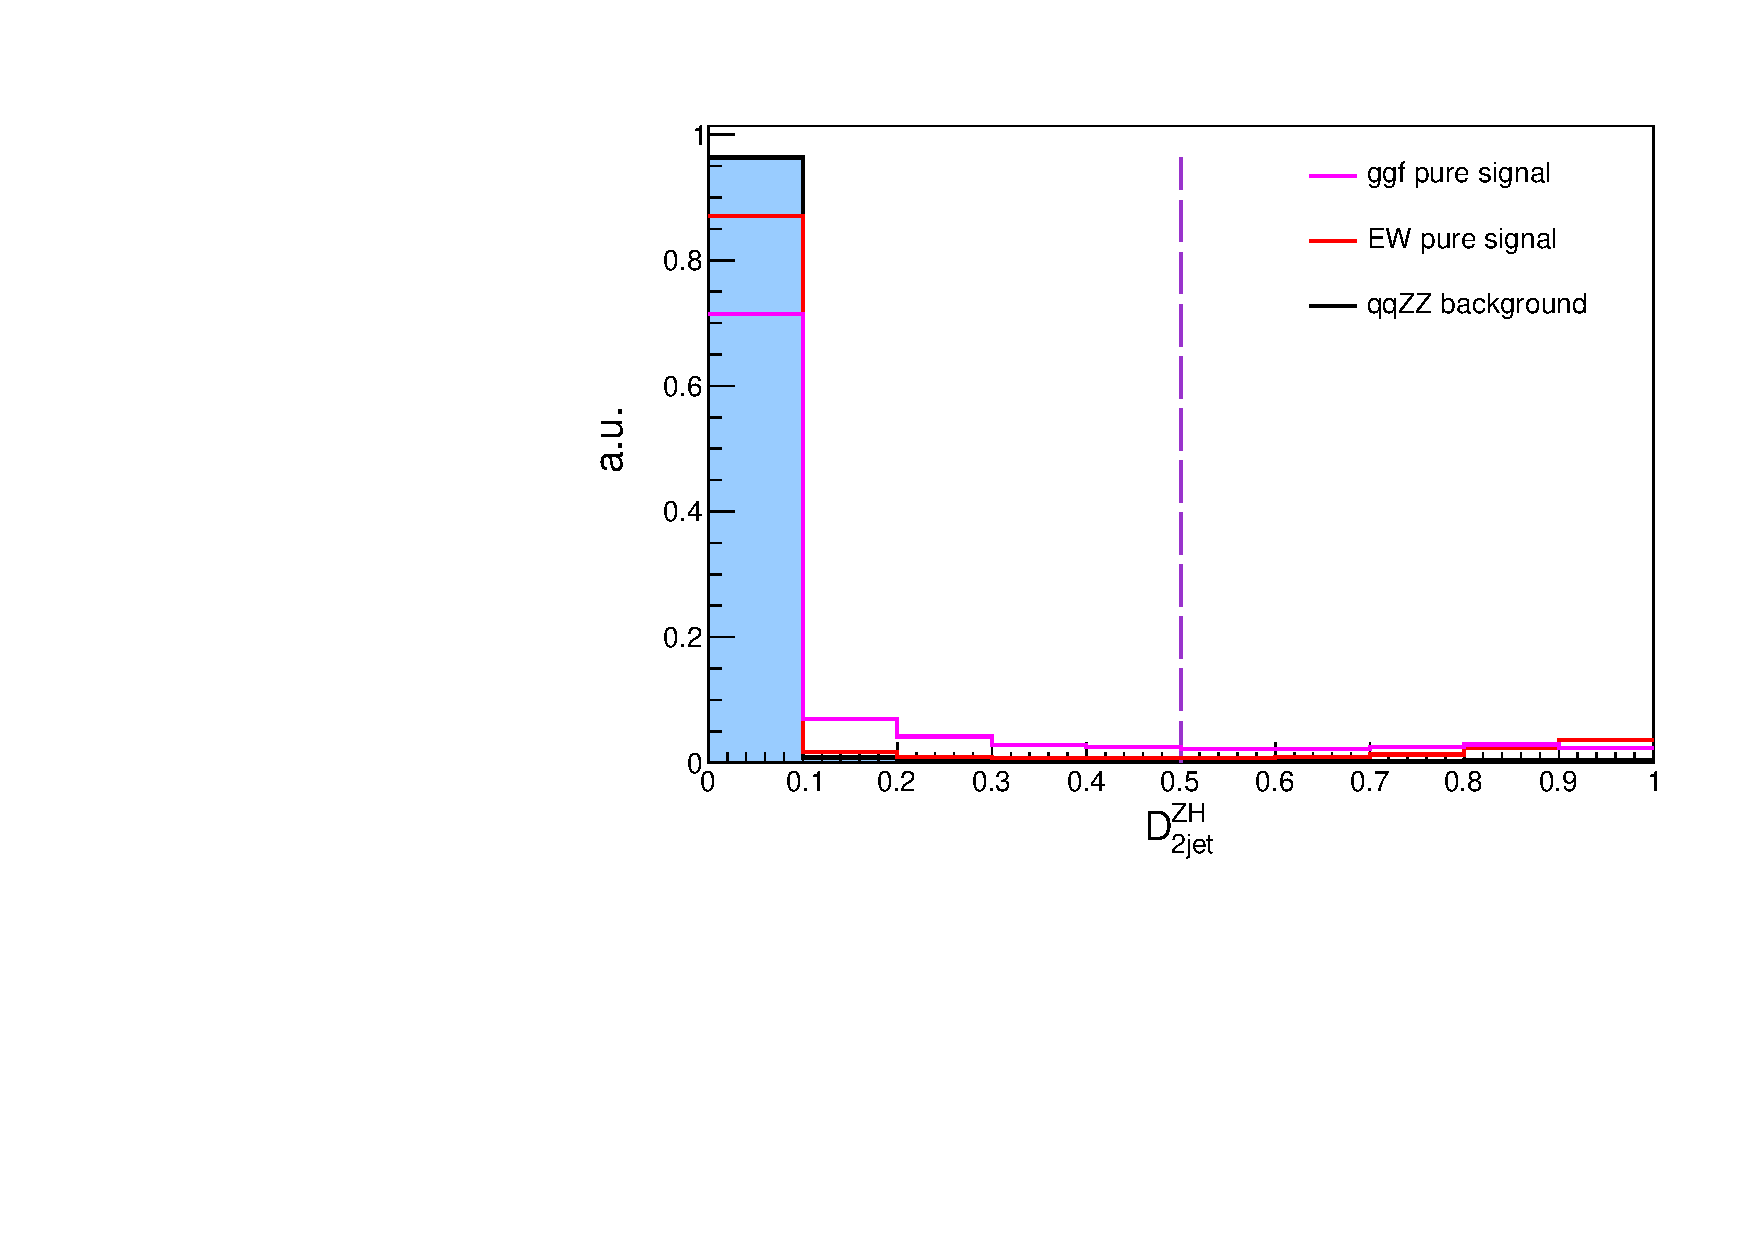
\includegraphics[width=0.8\textwidth]{figures/D2JZH_cat.pdf}
\caption{
Distribution of the $\mathcal{D}_\mathrm{2jet}^{ZH}$  discriminant used in selection of the VH-hadronic category. 
Three distributions are shown in the \offshell selection region ($m_{4\ell}>220$ GeV):
SM signal \offshell production in gluon fusion (JHUGen+MCFM, magenta); 
SM signal \offshell EW production, including VBF, ZH, and WH (JHUGen+MCFM, red); 
$q\bar{q}\to 4\ell$ background production (shaded). 
The selection threshold of 0.5 is shown with the dashed line. 
}
\label{fig:SelectionDiscriminant_D2jetZH}
\end{figure*}
%%%%%%%%%%%%%%%%%%%%%%%%%%%%%%%%%%%%%%%%%
%%%%%%%%%%%%%%%%%%%%%%%%%%%%%%%%%%%%%%%%%
\begin{figure*}[!hbt]
\centering
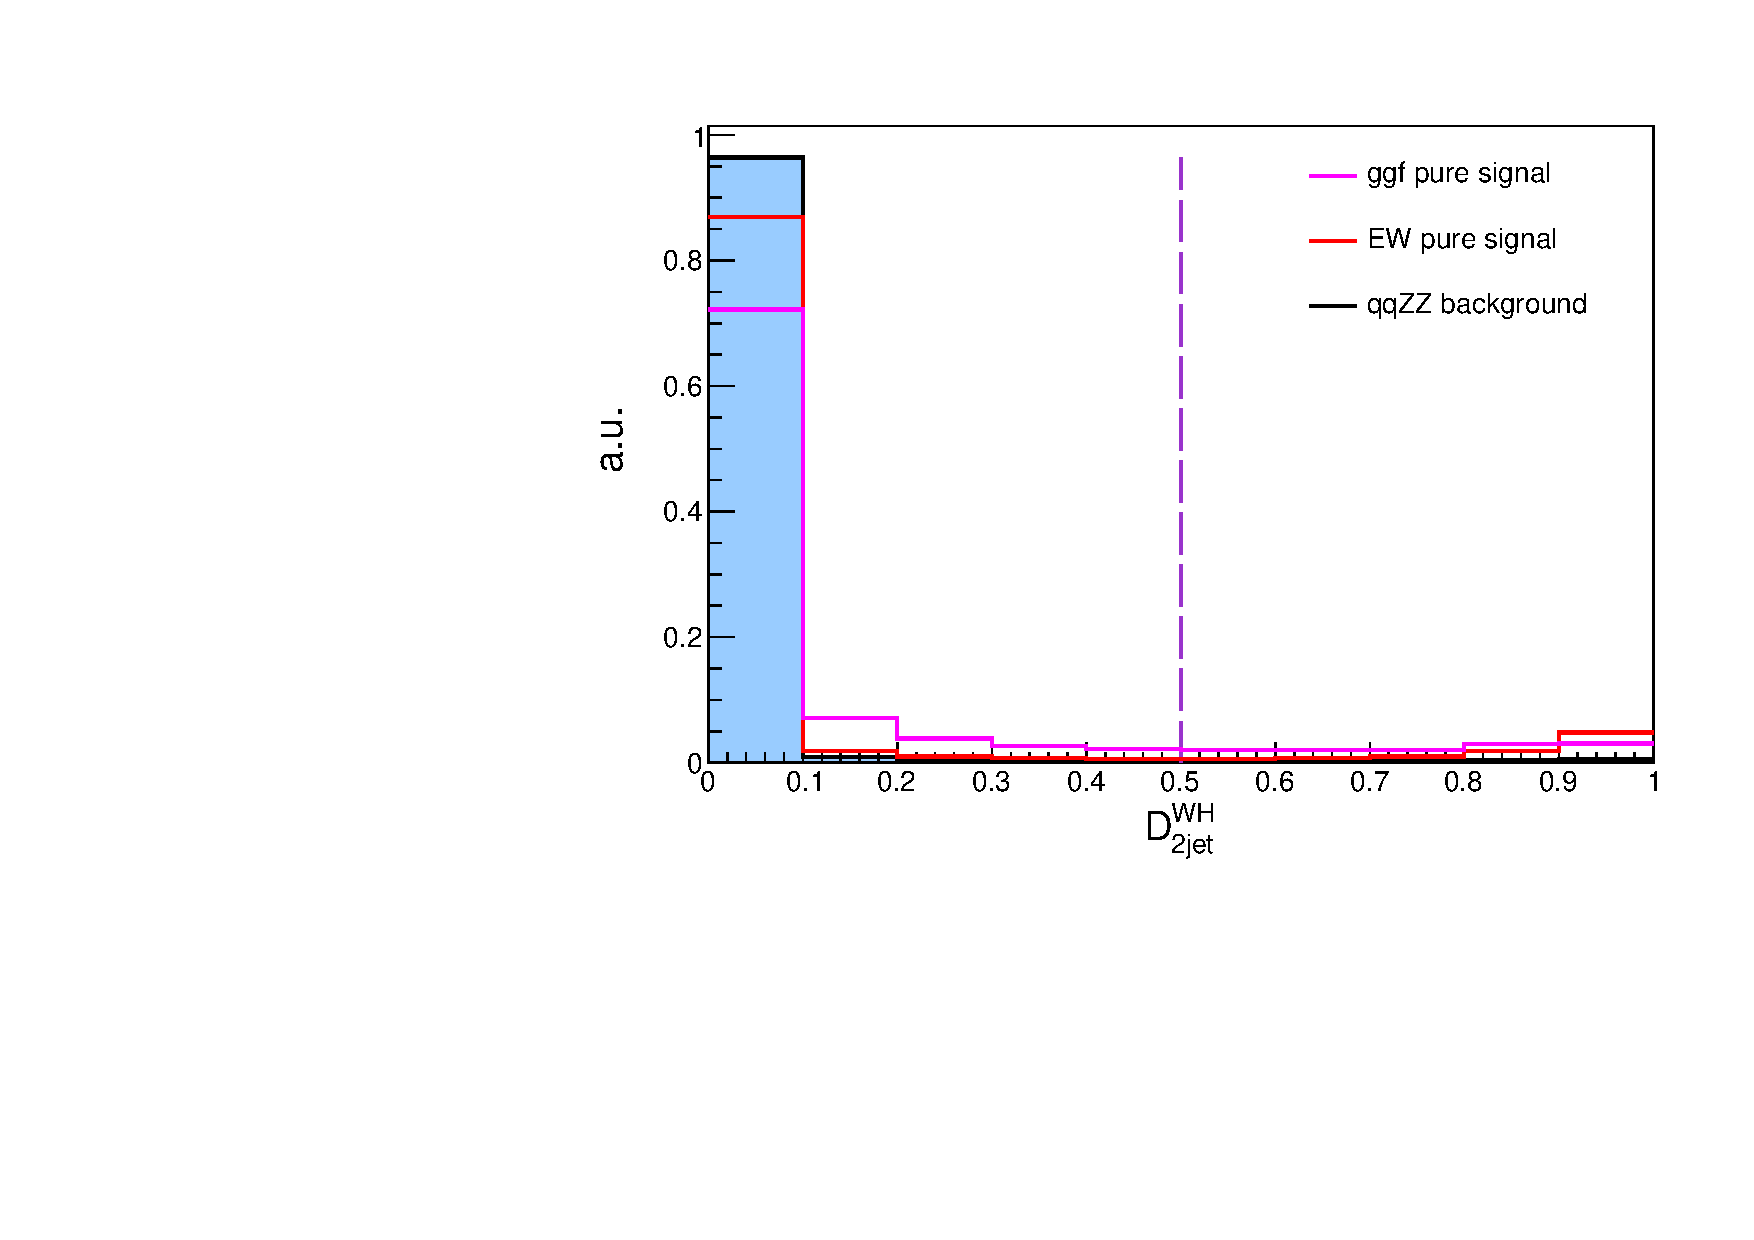
\includegraphics[width=0.8\textwidth]{figures/D2JWH_cat.pdf}
\caption{
Distribution of the $\mathcal{D}_\mathrm{2jet}^{WH}$  discriminant used in selection of the VH-hadronic category. 
Three distributions are shown in the \offshell selection region ($m_{4\ell}>220$ GeV):
SM signal \offshell production in gluon fusion (JHUGen+MCFM, magenta); 
SM signal \offshell EW production, including VBF, ZH, and WH (JHUGen+MCFM, red); 
$q\bar{q}\to 4\ell$ background production (shaded). 
The selection threshold of 0.5 is shown with the dashed line. 
}
\label{fig:SelectionDiscriminant_D2jetWH}
\end{figure*}
%%%%%%%%%%%%%%%%%%%%%%%%%%%%%%%%%%%%%%%%%

In each event category, the observables $\vec{x} = \{ m_{4\ell}, \mathcal{D}_\text{bkg}, \mathcal{D}_\text{int} \}$ are defined following Equations \ref{eq:melaD} and \ref{eq:melaDint},
and as summarized in Table~\ref{tab:categoriesoffshell}. The $\mathcal{D}_\text{bkg}$ observable is calculated with category-dependent methodology. In the Untagged category,
$\mathcal{P}_\text{bkg}$ is evaluated for the dominant $q\bar{q}\to4\ell$ background process.  
The signal and background probabilities incorporate both the matrix element probability, derived from the four-lepton kinematics, and a probability density function for the four-lepton invariant mass ($m_{4\ell}$), which is parameterized using simulated events to account for detector effects. The Higgs boson mass is constrained to $m_{H} = 125.38$\,GeV~\cite{Sirunyan:2020xwk}. An illustrative example of the value of $\mathcal{D}^{\rm kin}_{\rm bkg}$ is shown in Figure~\ref{fig:DiscDist}.

In the VBF-tagged and VH-tagged categories, $\mathcal{P}_\text{bkg}$ and $\mathcal{P}_\text{sig}$ incorporate
not only four-lepton kinematics but also the kinematic properties of the two associated jets.
The $\mathcal{P}_\text{bkg}$ probability density characterizes the combined EW and QCD background processes $4\ell+2$\,jets,
while $\mathcal{P}_\text{sig}$ represents the EW processes VBF and VH. Inclusion of jet kinematics in the
$\mathcal{D}_\text{bkg}$ calculation enhances discrimination of the targeted signal production against both background and \Hboson production through gluon fusion.

The third observable, $\mathcal{D}_\text{int}$ defined in Equation \ref{eq:melaDint}, discriminates between the interference
of SM-like \Hboson coupling and background as an alternative model, and is designated
$\mathcal{D}_\text{bsi}$ for the signal-background interference in the off-shell region.
In the Untagged category, decay kinematic information is utilized in the calculation of $\mathcal{D}_\text{int}$.
In the VBF-tagged and VH-tagged categories, production information incorporating the two associated jets is employed.

% In each category of events, three observables $\vec{x}$ are defined following Equation \ref{eq:melaD} and \ref{eq:melaDint},
% and as summarized in Table~\ref{tab:categoriesoffshell}, $\vec{x} = \{ m_{4\ell}, \Dbkg, \Dint \}$.
% The \Dbkg observable is calculated differently in the three tagged categories. In the untagged category,
% $\mathcal{P}_\text{bkg}$ is calculated for the dominant $q\bar{q}\to4\ell$ background process.  
% The signal and background probabilities include the matrix element probability for a given $m_{4\ell}$ mass,
% as measured in experiment. 
% In the VBF-tagged and VH-tagged categories, $\mathcal{P}_\text{bkg}$ and $\mathcal{P}_\text{sig}$ include
% four-lepton kinematics and kinematic information of the two associated jets.
% The $\mathcal{P}_\text{bkg}$ probability density represents the EW and QCD background processes $4\ell+2$\,jets,
% while $\mathcal{P}_\text{sig}$ represents EW processes VBF and VH. It was found that jet kinematics in the
% \Dbkg calculation improves separation of the targeted signal production both against background
% and against the \Hboson gluon fusion production.

% The third observable, \Dint defined in Equation \ref{eq:melaDint}, separates the interference
% of the SM-like \Hboson coupling and background as an alternative model, and is called
% \Dbsi for the signal-background interference in the off-shell region.
% In the untagged category, decay information is used in the calculation of \Dint.
% In the VBF-tagged and VH-tagged categories, production information with the two associated jets is used.

\begin{figure}[!hbt]
\centering
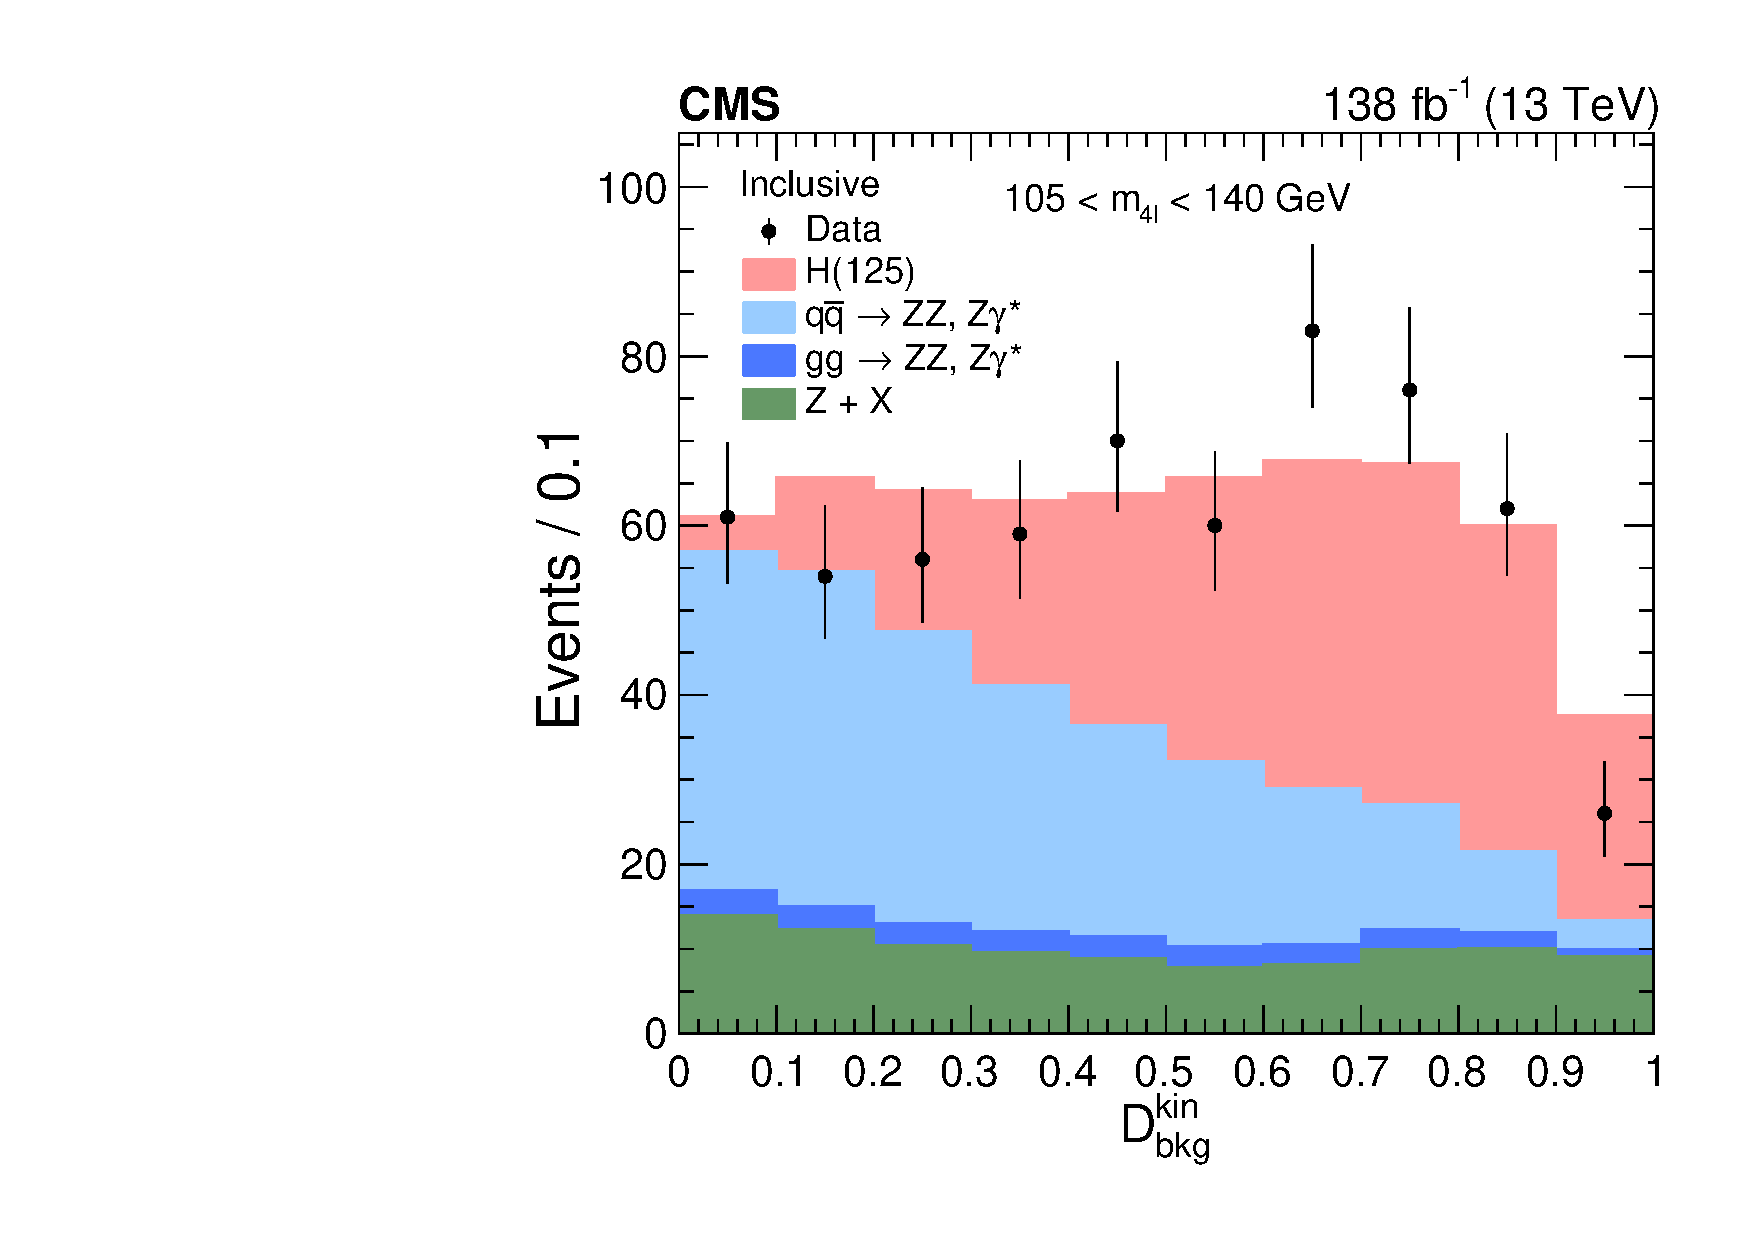
\includegraphics[width=0.8\textwidth,clip] {figures/Figure_004.pdf}
\caption{Distributions of the observed (points) and predicted (stacked histograms) \Dbkgkin of the four-lepton system, in the inclusive final state. The predictions for the \Hboson signal and the three main backgrounds are given by the different colors.  The vertical bars on the points show the statistical uncertainties in the data.}
\label{fig:DiscDist}
\end{figure}

% \begin{figure}[!hbt]
% \centering
% 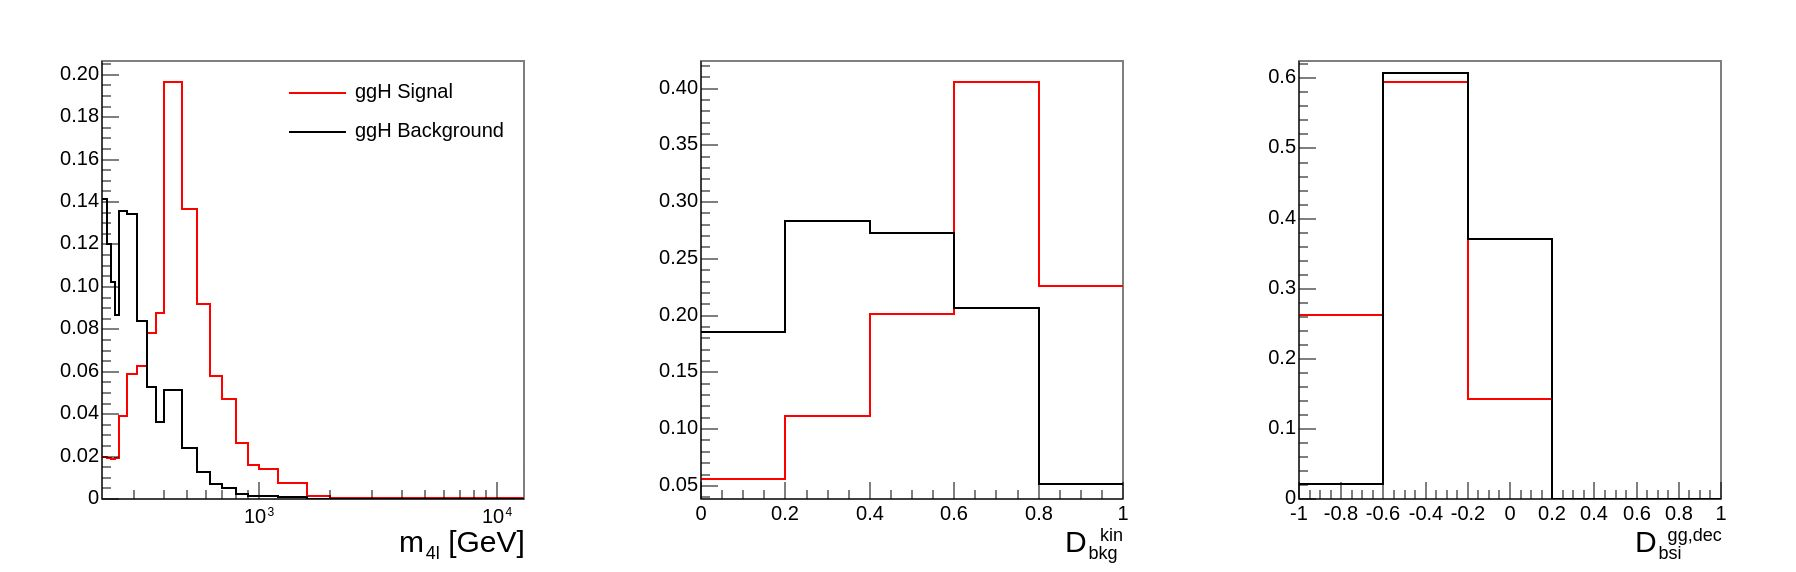
\includegraphics[width=0.8\textwidth,clip] {figures/DiscDists.jpg}
% \caption{}
% \label{fig:DiscDists}
% \end{figure}

The gluon fusion cross section is computed utilizing the highest-order QCD and electroweak (EW) expansions available for inclusive $ZZ$ production~\cite{deFlorian:2016spz}. 
However, event categorization relies on the modeling of associated jets through PYTHIA's parton showering and hadronization algorithms, which necessitates proper matching to the underlying hard-scattering process. Off-shell gluon fusion production is generated at leading order (LO) without associated jets at the matrix element level, implying that all reconstructed jets originate from PYTHIA's modeling. 
The parton showering and hadronization processes require specification of the hadronization scale, which is typically dependent on the characteristic energy scale of the process—set to $m_{4\ell}$ in the case of $gg\to 4\ell$.

For EW production mechanisms, the inclusive production cross section of $ZZ$ with two associated jets is similarly calculated using the highest-order QCD and EW expansions available~\cite{deFlorian:2016spz}. 
In contrast to gluon fusion, two hard jets—typically the leading jets in the event—are generated intrinsically at the matrix element level in the LO simulation. 
These jets correspond to either the forward-backward jets characteristic of vector boson fusion (VBF), or to the hadronic decay products of an associated W or Z boson. 
Consequently, the dependence on PYTHIA's parton shower and hadronization algorithms, and their matching to the hard-scattering production, is substantially reduced for these EW processes.

The categorization efficiency for simulated ggH and EW \Hboson production can be validated through comparison with alternative POWHEG and MINLO simulations. 
The POWHEG samples are generated across a broad range of off-shell \Hboson masses at next-to-leading order (NLO) in QCD, with one jet generated at the matrix element level and additional jets simulated through PYTHIA matching. 
The MINLO simulation of ggH production is performed for \Hboson masses of 125 and $300$ GeV at NLO in QCD, with two jets generated at the matrix element level and additional jets modeled via PYTHIA matching.

While JHUGen categorization efficiencies are consistent with those from POWHEG and MINLO within the uncertainties associated with the QCD scale implementation in PYTHIA,
the ggH process exhibits deviations in central values and corresponding uncertainties of up to 20\% in the signal-dominated $m_{4\ell}$ range of 300--500 GeV, with category-dependent variations. 
For EW processes, categorization efficiencies typically agree within 5--10\% between methodologies. 
We implement a correction procedure whereby the categorization efficiency as a function of $m_{4\ell}$ is adjusted to match that of the SM signal derived from POWHEG samples, with the assumption that this correction applies equally to background and interference contributions. 
This procedure ensures conservation of the total event yield across all three categories at each $m_{4\ell}$ value. An illustration of these categorization corrections can be found in Figure~\ref{fig:ew_catcor}.

\begin{figure*}[!hbt]
\centering
\includegraphics[width=0.85\textwidth]{figures/Corrections_allyears.pdf}
\caption {
Corrections as a function of $m_{4\ell}$ for \offshell EW process selection efficiencies in the Untagged, VBF-tagged, and VH-tagged categories. A polynomial fit is performed extending up to $2.5$ TeV. Events with $m_{4\ell}$ $ >  2.5$ TeV assume the correction value at the $2.5$ TeV cut-off. The correction is shown for the three data-taking periods in Run 2 combined.
\label{fig:ew_catcor}}
\end{figure*}

The simulation of the $\vec{x}$ observables enumerated in Table~\ref{tab:categoriesoffshell} remains unaffected by jet modeling in the Untagged category. Furthermore, the modeling of observables in jet-tagged categories for EW processes demonstrates remarkable consistency between direct MCFM+JHUGen samples and reweighted POWHEG+JHUGen implementations. 
However, jet modeling in jet-tagged categories for the ggH process significantly impacts the parametrization of probability distributions, as illustrated in Figures~\ref{fig:ggfmodvh} and \ref{fig:ggfmodvbf}.

\begin{figure*}[!hbt]
\centering
\includegraphics[width=0.45\textwidth]{figures/offggH_0PM_VHtagged_projy_0.pdf}
\includegraphics[width=0.45\textwidth]{figures/offggH_0PM_VHtagged_projy_2.pdf}\\
\includegraphics[width=0.45\textwidth]{figures/offggH_0PM_VHtagged_projz_0.pdf}
\includegraphics[width=0.45\textwidth]{figures/offggH_0PM_VHtagged_projz_2.pdf}\\
\caption {Comparison of $\mathcal{D}^{\rm VH+{\rm dec}}_{\rm bkg}$ and $\mathcal{D}^{\rm VH+{\rm dec}}_{\rm bsi}$ distributions between JHUGen and POWHEG for $m_{4\ell}>220$ GeV (left) and $250 < m_{4\ell} < 370$ GeV (right).}
\label{fig:ggfmodvh}
\end{figure*}

\begin{figure*}[!hbt]
\centering
\includegraphics[width=0.45\textwidth]{figures/offggH_0PM_VBFtagged_projy_0.pdf}
\includegraphics[width=0.45\textwidth]{figures/offggH_0PM_VBFtagged_projy_2.pdf}\\
\includegraphics[width=0.45\textwidth]{figures/offggH_0PM_VBFtagged_projz_0.pdf}
\includegraphics[width=0.45\textwidth]{figures/offggH_0PM_VBFtagged_projz_2.pdf}\\
\caption {Comparison of $\mathcal{D}^{\rm VBF+{\rm dec}}_{\rm bkg}$ and $\mathcal{D}^{\rm VBF+{\rm dec}}_{\rm bsi}$ distributions between JHUGen and POWHEG for $m_{4\ell}>220$ GeV (left) and $250 < m_{4\ell} < 370$ GeV (right).}
\label{fig:ggfmodvbf}
\end{figure*}

Therefore, within these two jet-tagged categories, the gluon fusion process is implemented through reweighted POWHEG+JHUGen simulation, which provides more precise parton shower matching and consequently superior modeling of associated jet activity. In this framework, samples are reweighted according to the appropriate theoretical model using the MELA package.

The observed and expected distributions of observables $\vec{x}$ for events in the \offshell region are illustrated in Figure~\ref{fig:ObservablesCat} for each of the three categories. The expected distributions are found using the SM predicted signal and background cross sections.

\begin{figure*}[!hbt]
\centering
\includegraphics[width=0.31\textwidth]{figures/Figure_005-a.pdf}
\includegraphics[width=0.31\textwidth]{figures/Figure_005-b.pdf}
\includegraphics[width=0.31\textwidth]{figures/Figure_005-c.pdf}\\ 
\includegraphics[width=0.31\textwidth]{figures/Figure_005-d.pdf}
\includegraphics[width=0.31\textwidth]{figures/Figure_005-e.pdf} 
\includegraphics[width=0.31\textwidth]{figures/Figure_005-f.pdf}\\ 
\includegraphics[width=0.31\textwidth]{figures/Figure_005-g.pdf}
\includegraphics[width=0.31\textwidth]{figures/Figure_005-h.pdf} 
\includegraphics[width=0.31\textwidth]{figures/Figure_005-i.pdf}\\ 
\caption{
Off-shell data (points) and pre-fit distributions (histograms) for the Untagged (left), VBF-tagged (middle), and VH-tagged (right) categories.
The upper row shows $m_{4\ell}$ distributions with a requirement on $\Dbkgkin>0.6$ (left), 
$\mathcal{D}^{{VBF}+{\text{dec}}}_\text{bkg}>0.6$ (middle), or $\mathcal{D}^{{VH}+{\text{dec}}}_\text{bkg}>0.6$ (right)
applied for illustration purposes to enhance signal over background contributions.
The middle row shows $\mathcal{D}^\text{kin}_\text{bkg}$ (left), $\mathcal{D}^{{VBF}+{\text{dec}}}_\text{bkg}$ (middle), $\mathcal{D}^{{VH}+{\text{dec}}}_\text{bkg}$ (right) distributions,
where an additional requirement $m_{4\ell}>340$ GeV is applied to enhance signal-over-background contributions.
The lower row plots the $\mathcal{D}_\text{bsi}$ with both the $m_{4\ell}$ and \Dbkgkin requirements specified above.
Contributions from the four processes are shown by the different colors, where ``s'', ``b'', and ``i'' refer to the 
signal, background, and interference contributions, respectively.
The vertical bars on the points give the statistical uncertainties in the data, and the horizontal bars represent the bin widths. 
For the pre-fit distributions, the different cross sections are set to their SM values~\cite{PhysRevD.111.092014}.
}
\label{fig:ObservablesCat}
\end{figure*}



% The gluon fusion cross section is calculated using the highest order QCD and EW expansions available 
% to simulate inclusive $ZZ$ production~\cite{deFlorian:2016spz}.
% However, event categorization depends on modeling associated jets through PYTHIA's parton showering and hadronization, 
% which involves matching these processes to the hard-scattering production. Off-shell gluon fusion production is generated at LO 
% with no associated jets at the matrix element level, and therefore all jets come from PYTHIA. 
% The parton showering and hadronization requires setting the hadronization scale, which can depend on the energy scale 
% in the process. In the case of the $gg\to 4\ell$ process, the energy scale is set at $m_{4\ell}$.

% The EW cross section for the inclusive production of $ZZ$ and two associated jets is also calculated to the highest order 
% QCD and EW expansion available~\cite{deFlorian:2016spz}. 
% Contrary to the gluon fusion process, two hard jets, which are typically the leading 
% jets in the process, are already generated at the matrix element level in the LO simulation. 
% These are the two associated jets in the VBF process, or 
% the two jets from the hadronic decay of the associated W or Z boson. 
% Therefore, the dependence on the PYTHIA parton shower and hadronization 
% and its matching to the hard-scattering production is much weaker for these EW processes. 

% The categorization efficiency of simulated ggH and EW \Hboson production can be checked using alternative POWHEG and MINLO simulations. 
% The POWHEG samples are generated for a wide range of off-shell \Hboson masses at NLO in QCD, 
% with one jet generated at the matrix element, and using PYTHIA matching to simulate additional jets. 
% The MINLO simulation of ggH production is done for \Hboson masses of 125 and $300$ GeV at NLO in QCD, 
% with two jets generated at the matrix element level, and PYTHIA matching for additional jets.
% While the JHUGen categorization efficiencies agree with those using POWHEG and MINLO 
% within the uncertainties of the QCD scale used in PYTHIA,
% for the ggH process the deviations of the central values and the corresponding uncertainties 
% are up to 20\% in the signal-dominated $m_{4\ell}$ range 300--500 GeV, depending on the category. 
% In the EW process, categorization efficiencies from the two approaches typically agree within 5--10\%. 
% In all cases, we adjust the categorization efficiency as a function of $m_{4\ell}$ to match that for the SM signal 
% obtained from the POWHEG samples, and assume the same behavior for 
% the background and interference contributions. 
% This correction procedure ensures that the total event yield, summed over the three categories,
% is unchanged at each value of $m_{4\ell}$.

% Simulation of the $\vec{x}$ observables listed in Table~\ref{tab:categoriesoffshell}
% is not affected by the jet modeling in the Untagged category. It is also found that the modeling
% of the observables in the jet-tagged categories is nearly the same in the EW process, when 
% compared between the direct MCFM + JHUGen samples and reweighted POWHEG + JHUGen. 
% However, the modeling of jets in the jet-tagged categories for the ggH process does impact 
% the parametrization of the probability distributions. Therefore, within these two jet-tagged categories, 
% the gluon fusion process is incorporated through the reweighted POWHEG + JHUGen simulation. 
% This approach allows a more precise matching with the parton shower, thereby 
% better describing the associated jet activity. In this case, the samples are reweighted for the appropriate 
% model using the MELA package.

\subsection{Modeling of Background}

The largest background in the $H \to 4\ell$ channel originates from the process $q\bar{q} \to ZZ/Z\gamma^*/\gamma^*\gamma^* \to 4\ell$. Additionally, the processes $gg \to ZZ/Z\gamma^*/\gamma^*\gamma^* \to 4\ell$ and electroweak (EW) production---including vector boson scattering and $VZZ$ processes---also contribute to the background and interfere with off-shell \Hboson production. In the \onshell region, this interference is negligible; however, the EW background additionally includes other processes such as $VVV$, $t\bar{t}VV$, and $t\bar{t}V$. 
% To model the invariant mass ($m_{4\ell}$) distribution for each irreducible background component, a third-order Bernstein polynomial is employed over the $m_{4\ell}$ range of 105--140\,GeV~\cite{PhysRevD.111.092014}.

Another important background arises from processes collectively referred to as $Z+X$, where leptons are misidentified from decays of heavy-flavor hadrons, in-flight decays of light mesons within jets, or charged hadrons overlapping with $\pi^0$ decays. The dominant contribution to this background is from $Z$+jets events, estimated using data-driven methods in dedicated control regions. These control regions are defined by selecting events containing one lepton pair meeting the ${Z}_{1}$ candidate requirements, along with an additional pair of opposite-sign leptons passing looser identification criteria compared to the main analysis selection. These four leptons must then satisfy the ${Z}_{1}, {Z}_{2}$ selection criteria. The background yield in the signal region is obtained by weighting the control region events by the lepton misidentification probability ($f_{\ell}$), defined as the probability for a non-prompt lepton to pass the analysis selection. A detailed description of this method can be found in Reference~\cite{Sirunyan:2017exp}. The $m_{4\ell}$ distribution for the $Z+X$ background is modeled by a Landau function, whose parameters are determined from data over an extended invariant mass range of 70--770\,GeV due to limited event counts.

The observed numbers of data events, expected backgrounds, and signal yields in the on-shell and off-shell regions are summarized in Tables~\ref{table:yields_SR} and \ref{tab:templateyields_offshell}, respectively. The signal and $ZZ$ background yields are derived from simulation, whereas the $Z+X$ background yield is obtained directly from data. Further details on the modeling of the \Hboson signal, interference effects with background processes, and $ZH$ cross-feed in the off-shell analysis are provided in Section~\ref{physicsmodel}.

\begin{table*}[!hbt] 
\centering
\begin{tabular}{lrrrrr}
   	&	$4\mu$	&	4e	&	$2e2\mu$	&	$2\mu2e$	& Total \\
\hline
Total signal    &       90.9    &       48.7    &       65.5    &       53.3    &       258.4   \\
$q\bar{q}\to4\ell$ background 	&	89.2	&	38.9	&	64.4	&	42.1	&	234.6	\\
$gg\to4\ell$ background	&	9.7	&	4.9	&	4.9	&	3.8	&	23.4	\\
$Z+X$ background	&	32.4	&	12.2	&	28.2	&	18.6	&	91.3	\\
Total expected	&	222.2	&	104.6	&	163.0	&	117.8	&	607.7	\\	
Observed	&	230	&	94	&	170	& 107	&	601	\\
\end{tabular}
\caption{The observed and expected yields for the \Hboson signal and background contributions in the \onshell region $105<m_{4\ell}<140$ GeV, for each of the four-lepton categories and the total~\cite{PhysRevD.111.092014}.}
\label{table:yields_SR}
\end{table*}

\begin{table*}[!hbt] 
\centering
\begin{tabular}{lrrrr}
& VBF-tagged & VH-tagged & Untagged & Total \\
\hline
$gg\to4\ell$ signal &1.0 & 0.9 & 25.1 & 27.0 \\
$gg\to4\ell$ background & 16.0 & 13.5 & 457.0& 486.4 \\
$gg\to4\ell$ interference & $-2.1$ & $-1.9$  &  $-52.0$ & $-56.1$ \\
EW signal         & 1.3 & 0.1 & 1.8& 3.2\\
EW background     & 14.9 & 2.9 & 19.7& 37.5\\
EW interference     & $-3.4$ & $-0.2$ & $-3.9$ & $-7.4$ \\
$ZH$ cross-feed & 0.2 & 0.4 & 7.0& 7.6 \\
$q\bar{q}\to4\ell$ background & 28.6 & 46.7 & 1795.1 & 1870.4  \\
$Z+X$ background & 4.7 & 5.3 & 89.7& 99.7  \\
Total expected & 61.2 & 67.8 & 2339.4 & 2468.4\\
Observed & 70 & 67 & 2335 & 2472 \\
\end{tabular}
\caption{Observed and expected yields for the \Hboson signal and background contributions 
in the \offshell region $m_{4\ell}> 220$ GeV, for each of the four-lepton categories and the total. 
The yields from interference of the signal and background and the $ZH$ cross-feed are also shown. 
The expected yields are adjusted within their respective uncertainties from the fit to the data~\cite{PhysRevD.111.092014}.}
\label{tab:templateyields_offshell}
\end{table*}

\subsection{Parameterizing the on-shell Higgs boson} \label{sec:onshell}

The probability density for the on-shell region includes both signal and background contributions.  It is normalized to the total event yield for each process $j$ and category $k$, and can be written as
\begin{equation}
  \mathcal{P}_{jk}(\vec{x};\vec{\xi}_{jk},\vec\zeta) = 
  \mu_j\mathcal{P}_{jk}^\text{sig} (\vec{x};\vec{\xi}_{jk},\vec\zeta) +
  \mathcal{P}_{jk}^\text{bkg}(\vec{x};\vec{\xi}_{jk}),
  \label{eq:ponshell}
\end{equation}
where $\vec\zeta$ are the unconstrained parameters of interest,
including the signal strength $\mu_j$ defined as the ratio of the signal yield to the SM expectation,
$\vec{\xi}_{jk}$ are the constrained nuisance parameters for a particular parametrization,
and $\vec{x}$ are the observables.

In the \onshell \Hboson mass and width analysis, six signal production processes are considered: ggH, VBF, VH, t$\bar{\text{t}}$H, b$\bar{\text{b}}$H, and tqH. The primary background contributions arise from three processes: $q\bar{q}/gg \to ZZ/Z\gamma^*/\gamma^*\gamma^* \to 4\ell$ and $Z+X$. 

When constraints on the total Higgs boson width ($\Gamma_H$) are extracted through a simultaneous fit to both the \onshell and \offshell regions, the \onshell component follows Scheme~2, as detailed in Reference~\cite{CMS:2021nnc}, which also provides further information on event categorization as well as signal and background modeling.

% For the \Hboson mass measurement, a one-dimensional (1D) statistical model is constructed in each category, for each signal production process, using the observable $m_{4\ell}$. The model is split by data-taking year and final state, and is further separated into nine bins of relative mass resolution ($\delta m_{4\ell}/m_{4\ell}$). 

% The signal shape for each process is obtained by fitting the simulated $m_{4\ell}$ distribution in the range 105--140\,GeV using a double-sided Crystal Ball function~\cite{Oreglia:1980cs}. For the VH and ttH production modes, a Landau function is included to model contributions where one of the leptons from the \Hboson decay falls outside the detector acceptance or fails the reconstruction and selection criteria. Our on-shell collaborators also utilized beam spot (BS) information, estimates of per-lepton momentum uncertainty, $m(Z_1)$ constraints, and the $\mathcal{D}^{\rm kin}_{\rm bkg}$ discriminant to provide the best on-shell Higgs boson mass and width precision, as we will see in Section~\ref{sec:results}~\cite{PhysRevD.111.092014}.

\subsection{Parameterizing the off-shell Higgs boson} \label{physicsmodel}

In the off-shell region, the probability density follows Equations~(\ref{eq:resonant}) and~(\ref{eq:ponshell}) closely,
with the additional contribution of the interference (``int'') between the signal and background amplitudes,
as well as a cross-feed (``cross'') component discussed below. It is parametrized as 
\begin{equation}\label{eq:poffshell}
    \mathcal{P}_{jk}(\vec{x};\vec{\xi}_{jk},\vec\zeta) =
    \frac{\mu_j \Gamma_H}{\Gamma_0}\mathcal{P}_{jk}^\text{sig} ( \vec{x};\vec{\xi}_{jk})
    + \sqrt{\frac{\mu_j \Gamma_H}{\Gamma_0}}\mathcal{P}_{jk}^\mathrm{int} ( \vec{x};\vec{\xi}_{jk})
    + \mu_j\mathcal{P}_{jk}^\text{cross} (\vec{x};\vec{\xi}_{jk})
    + \mathcal{P}_{jk}^\text{bkg} ( \vec{x};\vec{\xi}_{jk}),
\end{equation}
where $\Gamma_0$ is the reference value of the \Hboson width (not necessarily its SM value)
used in simulation. Otherwise, the definition of the terms is the same as in Equation~(\ref{eq:ponshell}). (Notably, $\mu_j$ is the signal strength on-shell.) 
In the off-shell width analysis, there are two production modes, $j$ (gluon fusion and EW, which includes both VBF and VH), 
and three jet-tagged categories, $k$. All lepton flavors and data periods are combined in this analysis.
The contributions from $t\bar{\text{t}}H$, $b\bar{\text{b}}H$, and $tqH$ are expected to be negligible at high energies.

The $\mathcal{P}_{jk}^{\text{sig}}$, $\mathcal{P}_{jk}^{\text{int}}$, $\mathcal{P}_{jk}^{\text{cross}}$, and $\mathcal{P}_{jk}^\text{bkg}$ probability densities are normalized to the expected number of events, and are implemented as binned histograms (templates) of the observables $\vec{x}$ listed in Table~\ref{tab:categoriesoffshell}. These templates are obtained as weighted linear combinations of existing simulated signal or background samples~\cite{PhysRevD.111.092014}.

\subsubsection{Cross-feed effect}

The \offshell region includes all events with $m_{4\ell} > 220$\,GeV. In this region, other processes can mimic off-shell \Hboson production and decay to four leptons. In particular, we consider \onshell Higgs boson events where the \Hboson decays to $2\ell + X$, where the $X$ can be replaced by mislabeled leptons which allow the event to satisfy the four-lepton selection criteria. The dominant \onshell \Hboson process that can contribute to the \offshell region is $Z(\ell\ell)H(2\ell + X)$, referred to as ZH cross-feed.

The ZH cross-feed contribution is estimated using \onshell ZH simulated samples with H $\to$ WW and ZZ decays, allowing for both hadronic and leptonic decays of the Z boson. The most significant contributions come from $H \to 2\ell 2\nu$ and $H \to 2\ell 2q$ final states, produced in association with $Z \to 2\ell$. Other possible contributions studied include the onshell t$\bar{\text{t}}$H production that contributes 0.57 events, and the ZH production of the Higgs boson with subsequent decay to two muons estimated to contribute $<$ 0.1 events. 

Templates for the statistical analysis are prepared using the \onshell ZH samples to model cross-feed
as a separate \onshell process. 
At the same time, to avoid double counting, \onshell cross-feed events are explicitly removed from the \offshell simulated samples.
% this cross-feed is removed from the \offshell modeling with the following procedure 
% using the MC truth information. 
Any simulated $H\to 2\ell 2q$ events in the \offshell EW JHUGen sample with mass close 
to the \Hboson pole mass within 100 MeV are removed. This procedure has close to 100\%
efficiency of selecting \onshell cross-feed events, while having a negligible effect on the other events. In addition to the ZH templates, the t$\bar{\text{t}}$H contribution is modeled and included in the statistical analysis. 

% In Figure~\ref{fig:crossfeed} (left) the $m_{4\ell}$ distribution of three samples is presented:
% \onshell cross-feed ZH(125) process, \offshell EW process with the cross-feed removed, 
% and the dominant $q\bar{q} \to 4\ell$ background process, which is scaled down by three
% orders of magnitude for easier visualization. The cross-feed and background processes exhibit similar distributions, while the genuine \offshell process has a more distinct shape with a dominant contribution at higher energies. The right plot shows the $m_{2\ell2q}$ mass distribution of events that are reconstructed in the \offshell region (Phantom sample). There is distinct narrow peak of \onshell cross-feed events at 125 GeV. A study of the categorization of the cross-feed events reveals the majority $(>91\%)$ end up in the Untagged category with the rest split between the two other event categories of the analysis. 
In Figure~\ref{fig:crossfeed} (left), the $m_{4\ell}$ distributions of three simulated samples are shown: the \onshell cross-feed process ZH(125), the genuine \offshell EW signal process with cross-feed contributions removed, and the dominant $q\bar{q} \to 4\ell$ background, which is scaled down by three orders of magnitude to facilitate comparison. The cross-feed and background processes exhibit similar kinematic distributions, while the genuine \offshell signal displays a distinct shape with a dominant contribution at higher invariant masses.

The right panel of Figure~\ref{fig:crossfeed} shows the $m_{2\ell2q}$ invariant mass distribution for events reconstructed in the \offshell signal region (plotted at MC-truth level). A narrow peak corresponding to the \onshell cross-feed component is clearly visible at 125\,GeV. A study of the event categorization reveals that the majority of these cross-feed events (\(>91\%\)) are classified into the Untagged category, with the remainder distributed between the VBF- and VH-tagged categories used in the analysis.

% Separate process with cross-feed events is defined in the likelihood fit, where these events are scaled with the \onshell signal strength. 

\begin{figure*}[!hbt]
\centering
\includegraphics[width=0.45\textwidth]{figures/M4L_proj_incl.pdf}
\includegraphics[width=0.52\textwidth]{figures/phantomm2l2q.pdf}
\caption {
Left: $m_{4\ell}$ distribution of \onshell cross-feed events, \offshell signal, and the dominant 
$q\bar{q} \to 4\ell$ background process (scaled down by three orders of magnitude).
Right: distribution of $m_{2\ell2q}$ for events reconstructed in the \offshell region 
of the $H\to 4\ell$ analysis. 
\label{fig:crossfeed}}
\end{figure*}

\subsection{Systematic Uncertainties}

Several systematic uncertainties are evaluated in the measurement of the constrained parameters $\vec{\xi}_{jk}$. The template shapes used to describe the probability distributions in Equations~(\ref{eq:ponshell}) and~(\ref{eq:poffshell}) are independently varied within their theoretical and experimental uncertainties. The resulting changes in the constrained parameters are taken as the systematic uncertainties associated with each source.

In the \onshell determination of the Higgs boson mass and width, the dominant systematic uncertainties arise from the lepton momentum scale and resolution. In the \offshell width measurement, the largest systematic uncertainty originates from the modeling of the dominant background process, $q\bar{q}/gg \to ZZ/Z\gamma^*/\gamma^*\gamma^* \to 4\ell$. Experimental uncertainties specific to the \offshell analysis include the jet energy calibration, which primarily affects the VBF- and VH-tagged categories.

Three sources of jet reconstruction-related uncertainties are studied and incorporated into the off-shell analysis. These include uncertainties in the jet energy scale (JES), jet energy resolution (JER), and the b-tagging scale factor. While the event categorization depends on the presence and properties of associated jets, the total event yield integrated over all three categories is not expected to vary significantly under these uncertainties. Instead, the dominant effect is a redistribution of events among the categories and corresponding changes in the shapes of the discriminant variables used within each.

To account for these effects, alternative calculations of the categorization discriminants and the jet-related logic (including the number of b-tagged jets) are performed for all variations of each uncertainty source. In addition, variations of the final observable discriminants are also computed. From these, up- and down-shifted templates are constructed and incorporated into the statistical analysis as systematic shape uncertainties.

Theoretical uncertainties impacting both the signal and background predictions include those associated with the renormalization and factorization scales, as well as the choice of parton distribution functions (PDFs). The uncertainty from the renormalization and factorization scales is estimated by varying both scales by factors of 0.5 and 2 relative to their nominal values, while maintaining the ratio between them within the range [0.5, 2]. PDF uncertainties are evaluated by computing the root mean square of variations across replicas of the default NNPDF set. An additional 10\% uncertainty is applied to the $K$ factor used in the ggZZ background prediction.

The integrated luminosities for the 2016, 2017, and 2018 data-taking periods carry individual uncertainties of 1.2--2.5\%~\cite{CMS-LUM-17-003,CMS-PAS-LUM-17-004,CMS-PAS-LUM-18-002}, with a combined uncertainty of 1.6\% for the full 2016--2018 dataset. The uncertainties in lepton identification, reconstruction, and selection efficiencies range from 2\% (for the $4\mu$ final state) to 14\% (for the $4e$ final state), affecting both signal and background yields.

For the estimation of the $Z + X$ background, differences in the flavor composition of hadronic jets misidentified as leptons between the $Z + 1\ell$ and $Z + 2\ell$ control regions introduce an uncertainty of approximately 30\% in the background yield. Additionally, uncertainties in the modeling of the misidentification rate as a function of $p_T$ and $\eta$, combined with the statistical uncertainty in the $Z + 1\ell$ control region, lead to total uncertainties in the background yields ranging from 32\% in the $4e$ final state to 39\% in the $4\mu$ final state.

An example impact plot of the nuisance parameters on the expected Higgs boson width result is presented in Figure~\ref{fig:impact}.

\begin{figure}[!hbt]
\begin{center}
\includegraphics[width=0.85\textwidth]{figures/impacts_all.pdf}
\caption
{
Expected impact of nuisance parameters on the Higgs boson width ratio to the SM value.
\label{fig:impact}
}
\end{center}
\end{figure}

\section{Measurement of Higgs boson properties} \label{sec:results}

\subsection{Higgs boson Width} \label{sec:offshellwidth}

% We perform an extended binned maximum likelihood fit to the on- and off-shell events split in several categories. The final measurements of $m_H$, $\Gamma_H$, and $\mu_{j}$ are conducted using the CMS statistical analysis tool COMBINE~\cite{CMS:2024onh}. 

% The extended likelihood function is constructed using the probability densities in Equations~(\ref{eq:ponshell}) and~(\ref{eq:poffshell}), with each event characterized by the discrete category $k$ and typically three observables $\vec{x}$. The likelihood $\mathcal{L}$ is maximized with respect to the nuisance parameters $\vec{\xi}_{jk}$ describing the systematic uncertainties and the signal strength parameter $\mu$ (total signal strength), or $\mu_F$ (signal strength for ggH) and $\mu_V$ (signal strength for the EW processes). The allowed 68 and 95\% CL intervals are defined using the profile likelihood function, $-2\Delta\ln\mathcal{L} = 1.00$ and $3.84$, respectively, for which exact coverage is expected in the asymptotic limit~\cite{Wilks:1938dza}.

% Constraints on $\Gamma_H$ are set by simultaneously fitting $H\to ZZ\to4\ell$ events from the on- and off-shell regions. The on-shell region corresponds to Scheme 2 in Reference~\cite{CMS:2021nnc}, where six mutually exclusive event categories are defined and anomalous interactions are constrained to zero. It determines two signal strengths, $\mu_j$ in Equations~(\ref{eq:ponshell}) and~(\ref{eq:poffshell}), 
% labeled as $\mu^\text{on-shell}_{F}$ and $\mu^\text{on-shell}_{V}$, which correspond to production mechanisms driven by fermion and vector boson couplings ofthe \Hboson, respectively. 
% The \Hboson mass is constrained to $m_H$=125.38 GeV \cite{Sirunyan:2020xwk} in this fit. 
% The observed and expected constraints on the \Hboson width are shown in Table~\ref{table:widthoffshellcomb}.
% The likelihood scan of $\Gamma_H$ using the asymptotic approximation method is shown in Figure~\ref{fig:widthscan}. 
% This measurement excludes the scenario of no off-shell \Hboson production with a CL corresponding 
% to 3.0 standard deviations (average expected 1.4).

An extended binned maximum likelihood fit is performed on the combined \onshell and \offshell event samples, divided into multiple analysis categories. The final measurements of $m_H$, $\Gamma_H$, and the signal strength parameters $\mu_{j}$ are carried out using the CMS statistical analysis tool COMBINE~\cite{CMS:2024onh}.

The extended likelihood function is constructed from the probability densities defined in Equations~(\ref{eq:ponshell}) and~(\ref{eq:poffshell}), where each event is characterized by a discrete category index $k$ and typically three observables $\vec{x}$. The likelihood $\mathcal{L}$ is maximized with respect to the nuisance parameters $\vec{\xi}_{jk}$, which encode systematic uncertainties, and the signal strength parameter $\mu$ (representing the total signal yield), or alternatively $\mu_F$ and $\mu_V$, corresponding to the gluon-fusion and electroweak production processes, respectively. Confidence intervals at 68\% and 95\% CL are determined using the profile likelihood method, with thresholds of $-2\Delta\ln\mathcal{L} = 1.00$ and $3.84$ ~\cite{Wilks:1938dza}.
% Confidence intervals at 68\% and 95\% CL are determined using the profile likelihood method, with thresholds of $-2\Delta\ln\mathcal{L} = 1.00$ and $3.84$, respectively, consistent with asymptotic coverage expectations~\cite{Wilks:1938dza}.

Constraints on $\Gamma_H$ are extracted from a simultaneous fit to $H \to ZZ \to 4\ell$ events in both the \onshell and \offshell regions. The \onshell region follows Scheme 2 as defined in Reference~\cite{CMS:2021nnc}, where six mutually exclusive categories are used and anomalous Higgs boson interactions are set to zero. This fit yields two signal strength parameters, $\mu^\text{on-shell}_{F}$ and $\mu^\text{on-shell}_{V}$, as defined in Equations~(\ref{eq:ponshell}) and~(\ref{eq:poffshell}), corresponding to production via fermionic and vector boson couplings of the \Hboson, respectively. The Higgs boson mass is fixed to $m_H = 125.38$\,GeV~\cite{Sirunyan:2020xwk}.

The observed and expected constraints on the Higgs boson width are presented in Table~\ref{table:widthoffshellcomb}, while the likelihood scan of $\Gamma_H$, obtained using the asymptotic approximation, is shown in Figure~\ref{fig:widthscan}. This measurement excludes the hypothesis of no off-shell Higgs boson production with a CL corresponding to 3.0 standard deviations (compared to an average expected 1.4).

The results of this analysis with the SM-like couplings are also combined with the prior CMS \offshell $H\to ZZ\to2\ell2\nu$ analysis~\cite{CMS:2022ley}, giving the first CMS measurement of $\Gamma_H$ using the full $4\ell$ and $2\ell2\nu$ data sample collected during Run 2. 
The observed and expected $\Gamma_H$ measurements are shown in Table~\ref{table:widthoffshellcomb} and Figure~\ref{fig:widthscan} and supersede the previous CMS results~\cite{CMS:2022ley} under the SM-like coupling assumption. These combined fit results rule out the scenario of no \offshell \Hboson production
with a CL corresponding to 3.8 standard deviations (average expected 2.4).

\begin{table*}[!thb]
    \centering
    % \renewcommand{\arraystretch}{1.25}
    \begin{tabular}{lll}
        Channel     & Observed $\Gamma_H$ (MeV)        &  Expected $\Gamma_H$ (MeV)  \\
        \hline
        $4\ell$ on- and off-shell    & $2.9^{+2.3}_{-1.7} \ [0.3,7.9]$ & $4.1\pm 4.0 \ [<11.5 ]$ \\
        $4\ell$ on- and off-shell  + $2\ell2\nu$ off-shell  & $3.0^{+ 2.0 }_{- 1.5 }  \ [0.6, 7.3]$ & $4.1\pm3.5 \ [0.1,10.5]$ \\
    \end{tabular}
    \caption{Summary of the total Higgs boson width $\Gamma_H$ measurement, showing the 68\%~CL (central values with uncertainties)
    and 95\%~CL (in square brackets) intervals for the $H \to ZZ \to 4 \ell$ channel alone and in combination with the off-shell $H \to ZZ \to 2 \ell 2 \nu$ channel~\cite{PhysRevD.111.092014}.}
    \label{table:widthoffshellcomb}
\end{table*}

\begin{figure}[!hbt]
    \centering
    \includegraphics[width=0.8\textwidth]{figures/Figure_011.pdf}  
    \caption{
        Observed (solid) and expected (dashed) profile likelihood projections from the \Hboson width fit using on- and off-shell production from this analysis. The analysis of the off-shell $H\to ZZ\to4\ell$ channel combined with the on-shell $H\to ZZ\to4\ell$ channel~\cite{CMS:2021nnc} is shown in black. The full combination of $H\to ZZ\to4\ell$ with the off-shell $H\to ZZ\to2\ell2\nu$~\cite{CMS:2022ley} is given in red. The black horizontal dashed lines show the 68 and 95\% CL values~\cite{PhysRevD.111.092014}.}
    \label{fig:widthscan} 
\end{figure}

% The observed limits on $\Gamma_H$ are stronger than the average expected values from simulation. 
% This is supported by our template plots, specifically the upper left plot of Figure~\ref{fig:ObservablesCat}, where the number of observed events in the sensitive region of $m_{4\ell}>340$ GeV and $\Dbkg > 0.6$ in the Untagged category is below the expected value (but still consistent). 

% The smaller number of events in this region favors the hypothesis of negative interference between the signal and background contributions, which dominates over the pure signal contributions for $\Gamma_H$ values near the SM value. Therefore, large and very small values of $\Gamma_H$ are disfavored.

The observed limits on $\Gamma_H$ are more stringent than the average expectations derived from simulation. This behavior is supported by the template distributions, in particular the upper-left panel of Figure~\ref{fig:ObservablesCat}, where the number of observed events in the region defined by $m_{4\ell} > 340$\,GeV and $\Dbkg > 0.6$ in the Untagged category is lower than expected, though still statistically consistent.

A reduced number of events in this sensitive region favors the hypothesis of greater negative interference between the signal and background contributions, which becomes dominant over the pure signal contributions for $\Gamma_H$ values near the SM value. As a result, both large and very small values of $\Gamma_H$ are disfavored by the data.

\subsection{Off-shell Signal Strength}

% The \offshell region fit can also be performed without relating its signal strength to that for the \onshell region.
% In this case, the signal strength is modified by the parameter $\mu^\text{off-shell}$ common to all production 
% mechanisms, with $\Gamma_H=\Gamma_H^{SM}$ in Eq.~(\ref{eq:poffshell}), and the SM expectation corresponding to $\mu^\text{off-shell}=1$. 
% In addition, we also perform a fit of the \offshell events with two unconstrained parameters $\mu^\text{off-shell}_{F}$ and
% $\mu^\text{off-shell}_{V}$, which express the signal strengths in the ggH and EW processes, respectively.
% The measured signal strengths are reported in Table~\ref{table:muoffshell} and a 2D scan of these parameters 
% is presented in Figure~\ref{fig:muoffshell}. The observed limits on signal strength in the \offshell region are stronger than expected on average, following a trend similar to that previously discussed for $\Gamma_H$.

An alternative approach to the \offshell region fit involves decoupling its signal strength from that of the \onshell region. In this configuration, the signal yield is scaled by a single parameter, $\mu^\text{off-shell}$, which is common to all production mechanisms. The total Higgs boson width is fixed to its SM value, $\Gamma_H = \Gamma_H^{\mathrm{SM}}$, in Equation~(\ref{eq:poffshell}), and the SM expectation corresponds to $\mu^\text{off-shell} = 1$. The likelihood scan for this parameter is presented in Figure~\ref{fig:1Dmus_off}.

In addition, a more general fit is performed with two unconstrained signal strength parameters: $\mu^\text{off-shell}_{F}$ and $\mu^\text{off-shell}_{V}$, corresponding to gluon-fusion and electroweak production mechanisms, respectively. The measured values of these parameters are reported in Table~\ref{table:muoffshell}, illustrated in Figures~\ref{fig:1Dmus_F} and \ref{fig:1Dmus_V}, and their joint CL regions are shown in the two-dimensional likelihood scan in Figure~\ref{fig:muoffshell}. The observed constraints on the \offshell signal strengths are stronger than the average expected values, consistent with the trend observed earlier in the $\Gamma_H$ analysis.

\begin{table*}[!hbt]
\centering
% \renewcommand{\arraystretch}{1.6}
\begin{tabular}{lcc}
  Parameter                & {Observed}          &  {Expected}   \\
  \hline
  $\mu^\text{off-shell}$ &  $0.67^{+ 0.42}_{-0.32 }\ [0.14,1.54]$ & $1.00^{+ 0.83}_{-0.84}\ [0.02,2.46]$ \\
  $\mu_F^\text{off-shell}$ &  $0.57^{+ 0.50}_{- 0.36}\ [0.04,1.61]$ & $1.00^{+0.90}_{-0.98}\ [{<}2.62]$\\
  $\mu_V^\text{off-shell}$ &  $ 0.87^{+0.93}_{-0.57}\ [0.05,2.90]$ & $1.00^{+1.95}_{-0.89}\ [{<}4.34]$ \\
\end{tabular}
\caption{
  Measured values of the signal strengths $\mu^\text{off-shell}$, $\mu_F^\text{off-shell}$, and $\mu_V^\text{off-shell}$,
  and their 68\% and 95\% (in square brackets) CL intervals from the combined fit to the \offshell $H\to ZZ\to4\ell$ and $2\ell2\nu$ channels.
}
\label{table:muoffshell}
\end{table*}

\begin{figure}[!hbt]
\begin{center}
\includegraphics[width=0.8\textwidth]{figures/scan_Roff_upd.pdf}
\caption
{
Observed and expected ikelihood scans for $\mu^{\text{off-shell}}$ with the combination of $H\to4\ell$ and $H\to2\ell2\nu$ final states.
\label{fig:1Dmus_off}
}
\end{center}
\end{figure}

\begin{figure}[!hbt]
\begin{center}
\includegraphics[width=0.8\textwidth]{figures/scan_muFoff_upd.pdf}
\caption
{
Observed and expected ikelihood scans for $\mu_F^{\text{off-shell}}$ with the combination of $H\to4\ell$ and $H\to2\ell2\nu$ final states.
\label{fig:1Dmus_F}
}
\end{center}
\end{figure}

\begin{figure}[!hbt]
\begin{center}
\includegraphics[width=0.8\textwidth]{figures/scan_muVoff_upd.pdf}
\caption
{
Observed and expected ikelihood scans for $\mu_V^{\text{off-shell}}$ with the combination of $H\to4\ell$ and $H\to2\ell2\nu$ final states.
\label{fig:1Dmus_V}
}
\end{center}
\end{figure}

\begin{figure}[!hbt]
  \centering
  \includegraphics[width=0.8\textwidth]{figures/Figure_012.pdf}  
  \caption
      {
        Observed 2D profile likelihood projection of the \offshell signal strength parameters ($\mu^\text{off-shell}_{F}$, $\mu^\text{off-shell}_{V}$) 
        from the fit to the combined \offshell $H\to ZZ\to4\ell$ and $2\ell2\nu$ channels. The best fit value is shown by the black cross and the SM 
        prediction by the red x. The 68 and 95\% CL contours are given by the dashed and solid curves, respectively. The color scale to the right of the plot relates the quantitative values~\cite{PhysRevD.111.092014}.
      }
    \label{fig:muoffshell} 
\end{figure}

\subsection{Kappa Framework}

% The above $\Gamma_H$ constraints assume the expected SM-like evolution of the \Hboson couplings over a large $m_{4\ell}$ range.
% The anomalous contributions to the $H{VV}$ vertex in EW production and \Hboson decay were evaluated in our earlier analyses 
% using a smaller data set~\cite{Sirunyan:2019twz,CMS:2022ley}, and the constraints on $\Gamma_H$ remained consistent.
% However, the predominance of the top quark in the ggH loop is assumed here and in our previous analyses. 
% If there are additional contributions, such as from yet undiscovered heavy particles, then the $m_{4\ell}$ evolution 
% in the \offshell region would be altered.

% To investigate the impact of large-mass yet undiscovered particles in the ggH loop,
% we introduce a new heavy quark $Q$ with an unconstrained coupling strength 
% $\kappa_{Q}$ in the likelihood parametrization, as described in Refs.~\cite{Gritsan:2020pib,Davis:2021tiv}.
% In the framework of effective field theories, the contribution of $Q$ can be interpreted 
% as a point-like interaction that encapsulates the influence of any heavy particles present in the loop.
% The parameterization in Equation~(\ref{eq:poffshell}) is extended to include the templates for terms proportional to 
% $\kappa^2_{Q}$ and $\kappa_{Q}$, utilizing simulations reweighted with the MELA package
% in the limit of the infinite $Q$ mass. 
% The $m_{4\Pell}$ shape in the \offshell region shows contrasting patterns between the SM ggH production, 
% which is mainly affected by the top quark loop with the $2m_{t}$ threshold effect, 
% and the \Hboson produced via ggH loop involving the heavy quark $Q$~\cite{Gritsan:2020pib}.

% An unconstrained $\kappa_{Q}$ introduces additional uncertainty into the $m_{4\ell}$ 
% dependence in the \offshell region, resulting in less stringent limits on $\Gamma_H$.
% However, both on- and \offshell $H\to4\ell$ data constrain the possible values of $\kappa_{Q}$, 
% and the constraints on $\Gamma_H$ remain largely consistent with those for $\kappa_{Q}=0$.
% The resulting $\Gamma_H$ measurement from the combined on- and \offshell events is $2.7^{+2.7}_{-1.8}$ MeV 
% (expected $4.1^{+5.5}_{-4.1}$ MeV). 
% The observed (expected) 95\%\, \CL interval is $\,[0.1,8.8]\, (\,[{<}14.4]\,)$ MeV.
% We note that combining measurements from other \onshell \Hboson production and decay channels 
% in the future will lead to much stricter constraints on $\kappa_{Q}$, reducing the flexibility 
% to alter the SM-like evolution of the \Hboson couplings over a large $m_{4\ell}$ range.

The $\Gamma_H$ constraints presented in Section~\ref{sec:offshellwidth} assume SM-like evolution of the Higgs boson couplings across a wide $m_{4\ell}$ range. Anomalous contributions to the $HVV$ vertex in EW production and Higgs boson decay were investigated in earlier analyses using smaller datasets~\cite{Sirunyan:2019twz,CMS:2022ley}, and the resulting $\Gamma_H$ constraints remained consistent. However, both the current and previous analyses assume that the gluon-fusion production mechanism is dominated by the top quark loop. If additional heavy particles contribute to the loop, this assumption would no longer hold, and the $m_{4\ell}$ dependence in the \offshell region could be significantly modified.

To explore the impact of potential contributions from new heavy particles in the $gg \to H$ loop, a hypothetical heavy quark $Q$ is introduced with an unconstrained coupling strength $\kappa_Q$, such as is described in Section~\ref{sec:kappa}~\cite{Gritsan:2020pib,Davis:2021tiv}. In the framework of Effective Field Theory (EFT), the influence of such a particle is modeled as a point-like interaction that encapsulates its loop effects. The parametrization in Equation~(\ref{eq:poffshell}) is extended to include template components proportional to $\kappa_Q$ and $\kappa_Q^2$, obtained from simulations reweighted using the MELA package in the limit of infinite $Q$ mass. 

The $m_{4\ell}$ distribution in the \offshell region exhibits different behaviors for SM-like gluon fusion—dominated by the top quark with the $2m_t$ threshold—and for scenarios involving the additional heavy quark $Q$~\cite{Gritsan:2020pib}. Allowing $\kappa_Q$ to vary freely introduces additional uncertainty in the $m_{4\ell}$ spectrum, which weakens the sensitivity to $\Gamma_H$. Nonetheless, both the \onshell and \offshell $H \to 4\ell$ data constrain the allowed values of $\kappa_Q$, and the $\Gamma_H$ constraints remain broadly consistent with the $\kappa_Q = 0$ case.

From the simultaneous fit to the \onshell and \offshell regions, the observed width is measured to be $\Gamma_H = 2.7^{+2.7}_{-1.8}$\,MeV, with an expected value of $4.1^{+5.5}_{-4.1}$\,MeV. The observed (expected) 95\% confidence interval is $[0.1,\,8.8]$\,MeV ($[\,{<}14.4]$\,MeV), as illustrated in Figure~\ref{fig:kappa_width_scan}. Future combinations with measurements from other \onshell Higgs boson production and decay channels are expected to significantly improve constraints on $\kappa_Q$, thereby reducing the allowed deviations from SM-like coupling evolution across the high-$m_{4\ell}$ regime.

\begin{figure}[!hbt]
    \centering
    \includegraphics[width=0.8\textwidth]{figures/Gamma_scan.pdf}
    \caption{
   Likelihood scan of the SM-like \Hboson width from Fig.~\ref{fig:widthscan} (black) as well as with $\kappa_Q$ unconstrained (blue).
    }
    \label{fig:kappa_width_scan}
\end{figure}

Utilizing Equations~\ref{eq:KappaMu} and \ref{eq:KappaMu2}, we can also consider likelihood scans of the parameters $\mu_F$ and $\mu_V$ in Figures~\ref{fig:kappa_muF_scan} and \ref{fig:kappa_muV_scan}, respectively, with and without including $\kappa_Q$ unconstrained. The numerical results are outlined in Table~\ref{table:offshellKappa}.\\

\begin{table}[!hbt]
\centering
% \renewcommand{\arraystretch}{1.25}
\begin{tabular}{llll}
\hline
Parameter       &     Configuration     & {Observed}          &  {Expected}   \\
\hline
$\mu_F$     & $\kappa_Q$ floated & $1.01^{+1.40}_{-0.41} ~[0.23,9.28]$   &  $1.00^{+5.49}_{-0.91} ~[0.80,1.21]$ \\
$\mu_F$     & $\kappa_Q=0$       & $0.87^{+0.09}_{-0.09} ~[0.69,1.08]$   &  $1.00^{+0.11}_{-0.10} ~[ < 15.88]$  \\
$\mu_V$     & $\kappa_Q$ floated & $1.05^{+0.44}_{-0.37} ~[0.35,1.98]$   &  $1.00^{+0.46}_{-0.40} ~[0.27,1.96]$  \\
$\mu_V$     & $\kappa_Q=0$       & $1.04^{+0.43}_{-0.37} ~[0.35,1.96]$   &  $1.00^{+0.46}_{-0.40} ~[0.27,1.96]$  \\
% $\kappa_Q$  & $\kappa_Q$ floated & $-0.06^{+0.28}_{-0.38} ~[-0.91,0.50]$ &  $0.00^{+0.58}_{-0.98} ~[-2.30,1.04]$  \\
% $\kappa_Q$  & $\kappa_Q=0$       & 0                                     &  0  \\
\hline
\end{tabular}
\caption{
Summary of constraints at 68\%~CL (central values with uncertainties) and 95\%~CL (in square brackets) on the parameters $\mu_F$ and $\mu_V$ with and without including $\kappa_Q$ unconstrained.}
\label{table:offshellKappa}
\end{table}

\begin{figure}[!hbt]
    \centering
    \includegraphics[width=0.8\textwidth]{figures/observed_muF.pdf}
    \caption{Observed and expected likelihood scans of $\mu_F$ with $\kappa_Q$ unconstrained (blue) and with $\kappa_Q=0$ (black).}
    \label{fig:kappa_muF_scan}
\end{figure}

\begin{figure}[!hbt]
    \centering
    \includegraphics[width=0.8\textwidth]{figures/observed_muV.pdf}
    \caption{Observed and expected likelihood scans of $\mu_V$ with $\kappa_Q$ unconstrained (blue) and with $\kappa_Q=0$ (black).}
    \label{fig:kappa_muV_scan}
\end{figure}

It is worth noting that the constraints on $\mu_V$ remains largely unaffected by $\kappa_Q$ being floated or fixed, whereas the constraints on $\mu_F$ exhibit significant variation. This is because the EW production mechanism, characterized by $\mu_V$, is independent of $\kappa_Q$, whereas the ggH process is strongly influenced by both $\kappa_Q$ and $\kappa_q$---the latter being related to $\mu_F$ through Equation~(\ref{eq:KappaMu2}).

% A strong correlation is therefore expected between $\kappa_Q$ and $\mu_F$, as both parameters directly affect the normalization of the gluon fusion signal. In fact, these two parameters become nearly degenerate in the on-shell signal strength parameterization given in Eq.~(\ref{eq:kg2}), since variations in one can be compensated by the other. However, the presence of top-initiated processes, such as $t\bar{t}H$ production, helps break this degeneracy and introduces sensitivity to $\mu_F$ that is not replicated by $\kappa_Q$ alone.

% The constraints on $\kappa_Q$ arise from a combination of on-shell and off-shell production processes. The characteristic shape of the off-shell region, particularly the positive interference with the background at higher $m_{4\ell}$ values—illustrated in Fig.~\ref{fig:kappaQ}—places additional restrictions on the allowed values of $\kappa_Q$. Nevertheless, the statistical power of the off-shell measurement remains limited, which in turn affects the overall confidence level of the constraint.


% \subsection{Other measurements}

% \subsubsection{On-shell Mass}

% As mentioned previously in Section~\ref{sec:onshell}, compared to the previous CMS on-shell \Hboson measurements in this channel~\cite{Sirunyan:2017exp}, the statistical and systematic uncertainties affecting $m_{H}$ have been reduced by our collaborators' inclusion of the beam spot in a refit of the muon tracks; adoption of an improved event categorization procedure; and detailed study of the lepton momentum scale and resolution~\cite{PhysRevD.111.092014}.

% % The \Hboson mass is measured, using on-shell production, by fitting the $m_{4\ell}$ distribution in the mass range $105< m_{4\ell} < 140$ GeV, using different likelihood models.
% % The results have been determined using the CMS statistical analysis tool COMBINE~\cite{CMS:2024onh}, 
% % which is based on the \textsc{RooFit}~\cite{Verkerke:2003ir} and \textsc{RooStats}~\cite{Moneta:2010pm} frameworks.\\

% % Table~\ref{table:Mass1Dresults} shows the mass measurements obtained from the 1D approach, where no further assumptions have been made. In comparison to the 1D model, the 1D$^{'}_\text{BS}$ model reduces the uncertainty by about 15\%. Implementing the $\delta m_{4\ell} / m_{4\ell}$ categorization then gives the $\mathcal{N}$--1D$'_\text{BS}$ model, which leads to an additional 10\% improvement. 
% % Finally, using the \Dkinbkg discriminant to reduce the background produces the $\mathcal{N}$--2D$'_\text{BS}$ model with another 4\% improvement.  

% Table~\ref{table:Mass_results} shows the resulting $m_{4\ell}$ measurements from our collaborators' complete procedure. All the measured $m_{4\ell}$ values from the different fits are statistically compatible, given their uncertainties and correlations. Figure~\ref{MassLikelihoodScan} displays the observed 1D likelihood scans as functions of $m_H$, from the fits for the different $4\ell$ categories and combined.

% Combining all the $m_{4\ell}$ final states and data-taking years, our final result is 
% $m_H = 125.04~\pm~0.11$ (stat)$~\pm~0.05$ (syst) = $125.04~\pm~0.12$ GeV.
% The largest systematic uncertainty is from the lepton momentum scale and equals 0.03 and 0.04 GeV for final states with muons and electrons, respectively.

% % \begin{table*}[!hbt]	
% %   \centering
% %   \topcaption{
% %     Best fit values for the mass of the \Hboson measured in the inclusive 4$\ell$ final state and separately for different flavor categories using the 1D approach.
% %     Uncertainties are separated into statistical and systematic uncertainties.
% %     Expected uncertainties are also given assuming $m_{H} = 125.38$ GeV \cite{Sirunyan:2020xwk}.
% %   }
% %   \renewcommand{\arraystretch}{1.6}
% %     \begin{tabular}{lcc}
% %       $4\ell$ category & Observed ($\pm$stat$\pm$syst) (GeV) & Expected uncertainty ($\pm$stat$\pm$syst)  (GeV) \\
% %       \hline
% %       Inclusive &	$124.98 \pm 0.14 \pm0.05$ & $ \pm 0.14 \pm 0.05$ \\
% %       $4\mu$ &	$124.87 \pm 0.17\pm0.04$ & $\pm 0.18 \pm 0.04$ \\
% %       $2\mu2e$ &	$125.32^{+0.36}_{-0.37}\pm0.10$ & $^{+0.34+0.09}_{-0.34-0.10}$ \\
% %       $2e2\mu$ &        $125.23^{+0.36+0.09}_{-0.35-0.11}$ & $^{+0.35+0.09}_{-0.35-0.10}$ \\
% %       ${4e}$ &    $124.94^{+0.68}_{-0.71} \pm 0.20$ & $^{+0.51+0.18}_{-0.51-0.20}$ \\
% %   \end{tabular}
% %   \label{table:Mass1Dresults}
% % \end{table*}

% \begin{table*}[!hbt]	
%   \centering
%   % \renewcommand{\arraystretch}{1.6}
%     \small
%     \begin{tabular}{lccc}
%       $4\ell$ category & Observed ($\pm$stat$\pm$syst) (GeV) & Expected uncertainty ($\pm$stat$\pm$syst) (GeV)  \\
%       \hline
%       Inclusive  & $125.04\pm0.11 \pm 0.05$	&	 $\pm 0.11\pm  0.05$ \\
%       $4\mu$ & $124.90 \pm 0.14 \pm 0.05$	&	$\pm 0.14\pm  0.04$ \\
%       $2e2\mu$ &        $125.50^{+0.25}_{-0.24}\pm0.10$      &       $\pm0.24\pm0.10$ \\
%       $2\mu2e$ &        $125.20^{+0.27+0.11}_{-0.26-0.07}$     &        $\pm0.27\pm0.10$ \\
%       $4e$ &	$124.70^{+0.49}_{-0.47}\pm0.20$     &	$\pm0.38\pm0.20$ \\ 
%   \end{tabular}
%   \caption{Best fit values for the mass of the \Hboson measured in the inclusive 4$\ell$ final state and separately for different flavor categories, using the final fit configuration~\cite{PhysRevD.111.092014}. Uncertainties are separated into statistical and systematic uncertainties. Expected uncertainties are also given assuming $m_{H} = 125.38$ GeV~\cite{Sirunyan:2020xwk}.}
%   \label{table:Mass_results}
% \end{table*}

% \begin{figure}[!hbt]
%   \centering
%   \includegraphics[width=0.8\textwidth]{figures/Figure_008.pdf}
%   \caption{The profile likelihood from the $m_H$ fit using the comprehensive on-shell model for each of the 4$\ell$ categories and combined.  The change in likelihood corresponding to 68 and 95\% CLs are shown by the dashed horizontal lines. Both statistical and systematic uncertainties are included in the fits~\cite{PhysRevD.111.092014}.}
%   \label{MassLikelihoodScan}
% \end{figure}

% % As a check on the analysis technique and the systematic uncertainty from this method, the 
% % 1D$^{'}_\text{BS}$ model is applied to $Z \to 4\ell$ events in the $m_{4\ell}$ range 70--105  GeV. The signal shape is obtained using a convolution of a Breit--Wigner function and a double-sided Crystal Ball function.
% % The fitted values of $m_Z$ in different subchannels are $m_Z^{4\mu} = 91.02 \pm 0.14$ GeV, $m_Z^{4e} = 91.18 \pm 0.45$ GeV, $m_Z^{2e2\mu} = 91.40 \pm 0.29$ GeV, and $m_Z^{2\mu2e} = 91.40 \pm 0.37$ GeV, leading to a combined value of $m_Z = 91.17 \pm 0.12$ GeV, consistent with the world-average Z boson mass~\cite{Agashe:2014kda} and with the uncertainty in agreement with the expected value of $\pm~0.12$ GeV from simulation.

% The results from this analysis are combined with those extracted using data recorded with the  
% CMS detector during Run 1 at $\sqrt{s}= 7$ and 8 TeV~\cite{Chatrchyan:2013mxa}. 
% Since this analysis uses an improved method to extract the systematic uncertainties affecting lepton momentum, 
% the lepton energy scales and resolution uncertainties are considered uncorrelated between the two runs. The combined observed result from both data-taking periods is $m_H$ = 125.08 $\pm$ 0.10 (stat) $\pm$ 0.05 (syst) GeV = 125.08 $\pm$ 0.12 GeV. Figure~\ref{Run1Run2_scan} presents a summary of the \Hboson mass measurements by the CMS Collaboration in the four-lepton decay channel.
%  % The corresponding expected statistical and systematic uncertainties are $\pm$0.10 and $\pm$0.05 GeV, respectively.
% \begin{figure*}[!hbt]
%   \centering
%   \includegraphics[width=0.8\textwidth]{figures/Figure_009.pdf}
%   \caption{Summary of the CMS Higgs boson mass measurements using the four-lepton final state. The red vertical line and the gray column represent the best fit value and the total uncertainty, respectively, as measured by combining Run 1 and Run 2 data. The yellow band and horizontal black bars show the statistical and total uncertainties in each measurement, respectively. The value of each measurement is given, along with the total and statistical only (in parentheses) uncertainties~\cite{PhysRevD.111.092014}.}
%   \label{Run1Run2_scan}
% \end{figure*}

% \subsubsection{On-shell Width}

% The final \onshell model is also used for an on-shell-only Higgs boson width measurement, with the signal model extended to include the $\Gamma_H$ parameter. Since the theoretical prediction for $\Gamma_H$ is very close to zero---a strict lower bound---confidence intervals are constructed using the Feldman-Cousins approach~\cite{FC}. The confidence level (CL) was evaluated by our collaborators for various width hypotheses using distributions derived from simulated pseudo-experiments~\cite{PhysRevD.111.092014}.

% The observed (expected) upper limit on $\Gamma_H$ is 50\,(320)\,MeV at 68\% CL and 330\,(640)\,MeV at 95\% CL. Although the observed limit is significantly lower than the expected one, both are statistically compatible. The resulting distribution of 1-CL as a function of $\Gamma_H$ is shown in Figure~\ref{OnShell_width}. This measurement is statistically limited; the dominant uncertainty arises from statistical fluctuations, while the leading systematic uncertainty is driven by the lepton momentum resolution.

% \begin{figure}[!hbt]
%   \centering
%   \includegraphics[width=0.8\textwidth]{figures/Figure_010.pdf}
%   \caption{Distribution of 1-CL versus $\Gamma_H$ from the fit used to measure the Higgs boson width using on-shell production only. The CL values shown by the points are extracted using the Feldman-Cousins approach. The vertical bars on the points represent the spread in the simulated pseudo-experiment outcomes. The 68\% and 95\% CL thresholds are indicated by the dashed horizontal lines~\cite{PhysRevD.111.092014}.}
%   \label{OnShell_width}
% \end{figure}

\chapter{Conclusion} \label{chap:chap-5}

This thesis is centered around precision measurements of the Higgs boson properties (width) using the $H^{(*)} \to ZZ^{(*)} \to 4\ell$ decay channel in proton-proton collisions at $\sqrt{s} = 13$\,TeV collected by the CMS experiment, corresponding to an integrated luminosity of 138\,fb$^{-1}$. The strength of off-shell Higgs production is also measured, excluding the no off-shell production hypothesis at 3.8 standard deviations, after ReReco-based combination with $H \to ZZ \to 2\ell2\nu$. The published ReReco-based and latest UL-based results are summarized in Tables~\ref{table:widthoffshellcomb} and \ref{table:widthoffshellUL}, respectively.

A simultaneous fit to on- and off-shell production in the $4\ell$ final state, combined with results from the $2\ell2\nu$ final state, gives us our most data-inclusive measurement to date and yields $\Gamma_H = 3.0^{+2.0}_{-1.5}$\,MeV, consistent with the SM prediction of 4.1\,MeV. A $4\ell$-only measurement made with more recent UL processing returns $\Gamma_H = 3.4^{+2.6}_{-2.0}$\,MeV.
% Combining data from Runs 1 and 2 improves the mass measurement to $m_H = 125.08 \pm 0.10\,\text{(stat)} \pm 0.05\,\text{(syst)}\,$GeV$ = 125.08 \pm 0.12\,$GeV, the most precise single-channel result to date. 

These results provide stringent tests of the Standard Model and establish an experimental baseline for characterizing Higgs boson properties. Looking ahead, this analysis provides a robust foundation for future studies targeting deviations from SM expectations. The methods and statistical techniques developed here are directly extensible to searches for anomalous Higgs couplings and BSM effects in the $HVV$ vertex. This framework will support increasingly precise constraints as we move toward a Standard Model Effective Field Theory (SMEFT) description of the Higgs boson and probe Electroweak Symmetry Breaking (EWSB) to potentially uncover new physics.






% As larger datasets become available with Run 3, particularly including more statistics at higher energies, this framework will hopefully support increasingly precise constraints as we move toward a Standard Model Effective Field Theory (SMEFT) description of the Higgs boson. These studies are essential for probing the electroweak symmetry breaking mechanism and for uncovering potential signs of new physics.

% The precision achieved in this thesis reinforces the central role of the Higgs boson as a portal to new physics and sets the stage for future explorations into its interactions, structure, and possible extensions within the SMEFT paradigm.



% The mass is measured with an uncertainty of $\pm0.12$\,GeV, and the most precise single-channel measurement to date is achieved by combining Run~1 and Run~2 data: $m_H = 125.08 \pm 0.12\,\GeV$. The Higgs boson width is constrained to $\Gamma_H = 3.0^{+2.0}_{-1.5}\,\MeV$, consistent with the Standard Model prediction of $4.1\,\MeV$, and the hypothesis of no off-shell Higgs boson production is excluded at the level of 3.8 standard deviations. 
% Combining data from Runs 1 and 2 improves the mass measurement to $m_H = 125.08 \pm 0.10\,\text{(stat)} \pm 0.05\,\text{(syst)}\,\GeV = 125.08 \pm 0.12\,\GeV$, the most precise single-channel result to date. A simultaneous fit to on- and off-shell production in the four-lepton final state, combined with results from $H \to 2\Pell2\PGn$, yields $\Gamma_H = 3.0^{+2.0}_{-1.5}\,\MeV$, consistent with the SM prediction of 4.1\,MeV.


% A measurement of the Higgs boson mass ($m_H$) and width ($\Gamma_H$) is presented using $\PH \to \PZ\PZ \to 4\Pell$ decays ($\Pell = \Pe,\,\PGm$) in proton-proton collisions at $\sqrt{s} = 13\,\TeV$, recorded by the CMS experiment with an integrated luminosity of 138\,fb$^{-1}$. The mass is measured using on-shell events, yielding $m_H = 125.04 \pm 0.11\,\text{(stat)} \pm 0.05\,\text{(syst)}\,\GeV = 125.04 \pm 0.12\,\GeV$, consistent with the expected precision. A 95\% confidence level upper limit of $\Gamma_H < 330\,\MeV$ is obtained from on-shell production.

% Combining data from Runs 1 and 2 improves the mass measurement to $m_H = 125.08 \pm 0.10\,\text{(stat)} \pm 0.05\,\text{(syst)}\,\GeV = 125.08 \pm 0.12\,\GeV$, the most precise single-channel result to date. A simultaneous fit to on- and off-shell production in the four-lepton final state, combined with results from $H \to 2\Pell2\PGn$, yields $\Gamma_H = 3.0^{+2.0}_{-1.5}\,\MeV$, consistent with the SM prediction of 4.1\,MeV. The results are summarized in Table~\ref{table:widthoffshell}. The strength of off-shell Higgs production is also measured, excluding the no off-shell production hypothesis at 3.8 standard deviations. Full results are available in the associated HEPData record~\cite{hepdata}.


% \section{Further Constraining Anomalous Behavior}

% \subsection{EFT and SMEFT}



% \subsection{Composition and Self-coupling}



% \section{Precision Measurements of the Higgs Boson}

% \lipsum[4]

%% add more main text technical chapters if you have

%%%%%%%%%%%%%%%%%%%%%%%%%%% END MAIN MATTER %%%%%%%%%%%%%%%%%%%%%%%%%%%%



%%%%%%%%%%%%%%%%%%%%%%%%%%%%% BACK MATTER %%%%%%%%%%%%%%%%%%%%%%%%%%%%%%

%%%% BIBLIOGRAPHIC REFERENCES
\BibTextSpacing                         % text spacing for each bib item
\fancyhead[L]{\nouppercase \leftmark}
\printbibliography[title={Bibliographic references},
    heading=bibintoc, notcategory=mypapers]
\clearpage                              % flushes out floating header


%%%% Appendix chapter (same header format as the main chapters)
%% if you do not have appendix chapters, then comment them out
\MainTextSpacing                    
\fancyhead[L]{\appendixname\ \thechapter. \nouppercase \leftmark}


% \include{11-appendix-A}
% \include{12-appendix-B}

%% add more appendix chapters if you have 

%%%%%%%%%%%%%%%%%%%%%%%%%%% END BACK MATTER %%%%%%%%%%%%%%%%%%%%%%%%%%%%

\end{document}

%%%%%%%%%%%%%%%%%%%%%%%%% DOCUMENT ENDS HERE %%%%%%%%%%%%%%%%%%%%%%%%%%%